\documentclass[letterpaper,12pt]{article}
\usepackage[english]{babel}
\usepackage[utf8x]{inputenc}
\usepackage[T1]{fontenc}
\usepackage{titlesec}
\usepackage[letterpaper,top=1in,bottom=1in,left=1in,right=1in,marginparwidth=0in]{geometry}
\usepackage{times}
\usepackage{amsmath}
\usepackage{graphicx}
\usepackage[colorlinks=true, allcolors=blue]{hyperref}
\usepackage{enumitem} 
\usepackage{natbib} 
\usepackage{libertine}
\usepackage{float}
\begin{document}
\fontfamily{ptm}\selectfont
\urlstyle{same}
\urlstyle{rm}
\tableofcontents
\pagebreak




% Time series for each predictor variable 

\subsection{ML Inputs (with NAs) Time Series Images} 
 

\begin{figure} 
\centering  
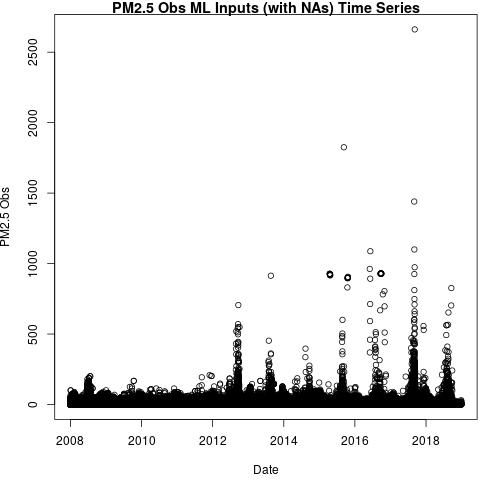
\includegraphics[width=0.77\textwidth]{Code_Outputs/Report_ML_input_PM25_Step4_part_e_de_duplicated_aves_compiled_2019-05-21wNAs_PM25_ObsvDate.jpg} 
\caption{\label{fig:Report_ML_input_PM25_Step4_part_e_de_duplicated_aves_compiled_2019-05-21wNAsPM25_ObsvDate}ML Inputs (with NAs) Time Series} 
\end{figure} 
 

\begin{figure} 
\centering  
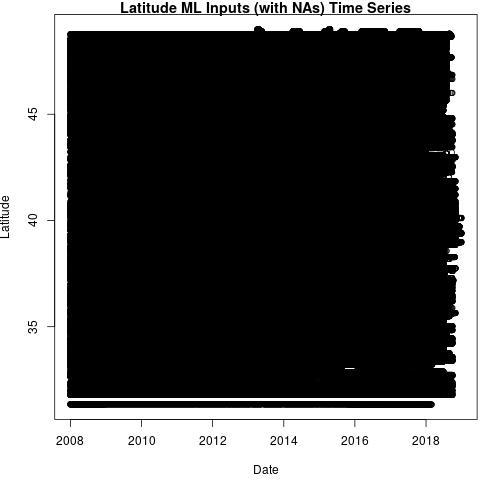
\includegraphics[width=0.77\textwidth]{Code_Outputs/Report_ML_input_PM25_Step4_part_e_de_duplicated_aves_compiled_2019-05-21wNAs_LatitudevDate.jpg} 
\caption{\label{fig:Report_ML_input_PM25_Step4_part_e_de_duplicated_aves_compiled_2019-05-21wNAsLatitudevDate}ML Inputs (with NAs) Time Series} 
\end{figure} 
 

\begin{figure} 
\centering  
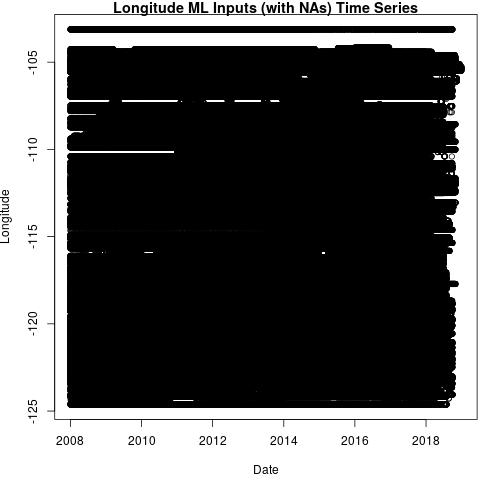
\includegraphics[width=0.77\textwidth]{Code_Outputs/Report_ML_input_PM25_Step4_part_e_de_duplicated_aves_compiled_2019-05-21wNAs_LongitudevDate.jpg} 
\caption{\label{fig:Report_ML_input_PM25_Step4_part_e_de_duplicated_aves_compiled_2019-05-21wNAsLongitudevDate}ML Inputs (with NAs) Time Series} 
\end{figure} 
 

\begin{figure} 
\centering  
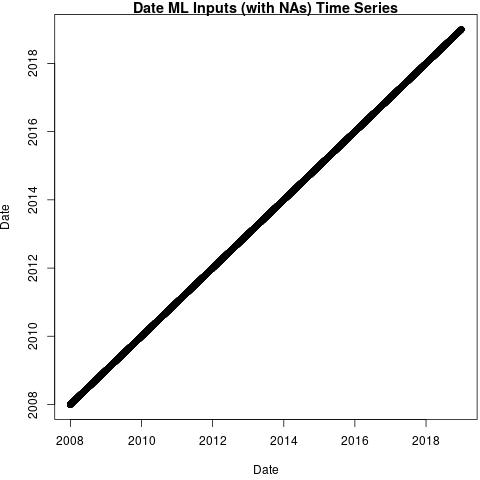
\includegraphics[width=0.77\textwidth]{Code_Outputs/Report_ML_input_PM25_Step4_part_e_de_duplicated_aves_compiled_2019-05-21wNAs_DatevDate.jpg} 
\caption{\label{fig:Report_ML_input_PM25_Step4_part_e_de_duplicated_aves_compiled_2019-05-21wNAsDatevDate}ML Inputs (with NAs) Time Series} 
\end{figure} 
 

\begin{figure} 
\centering  
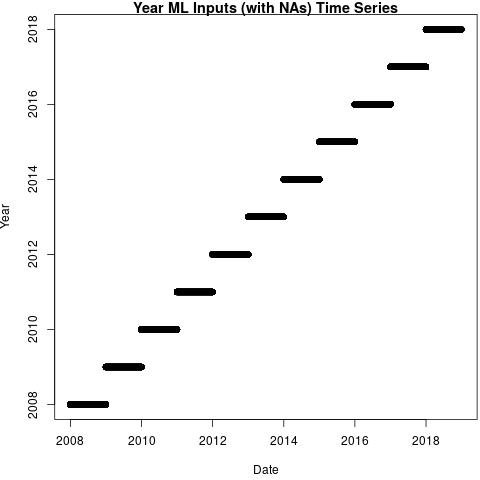
\includegraphics[width=0.77\textwidth]{Code_Outputs/Report_ML_input_PM25_Step4_part_e_de_duplicated_aves_compiled_2019-05-21wNAs_YearvDate.jpg} 
\caption{\label{fig:Report_ML_input_PM25_Step4_part_e_de_duplicated_aves_compiled_2019-05-21wNAsYearvDate}ML Inputs (with NAs) Time Series} 
\end{figure} 
 

\begin{figure} 
\centering  
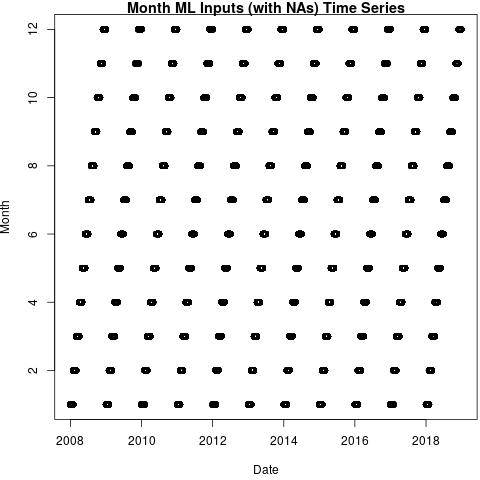
\includegraphics[width=0.77\textwidth]{Code_Outputs/Report_ML_input_PM25_Step4_part_e_de_duplicated_aves_compiled_2019-05-21wNAs_MonthvDate.jpg} 
\caption{\label{fig:Report_ML_input_PM25_Step4_part_e_de_duplicated_aves_compiled_2019-05-21wNAsMonthvDate}ML Inputs (with NAs) Time Series} 
\end{figure} 
 

\begin{figure} 
\centering  
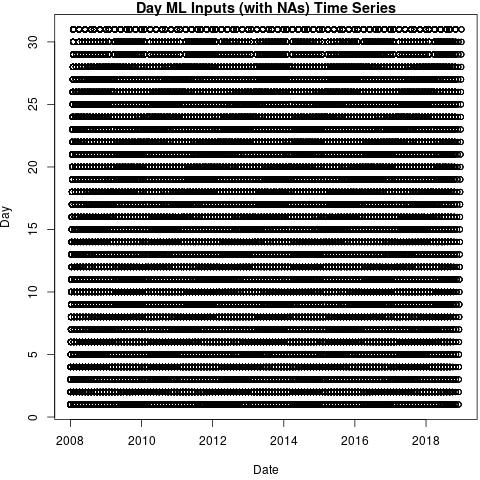
\includegraphics[width=0.77\textwidth]{Code_Outputs/Report_ML_input_PM25_Step4_part_e_de_duplicated_aves_compiled_2019-05-21wNAs_DayvDate.jpg} 
\caption{\label{fig:Report_ML_input_PM25_Step4_part_e_de_duplicated_aves_compiled_2019-05-21wNAsDayvDate}ML Inputs (with NAs) Time Series} 
\end{figure} 
 

\begin{figure} 
\centering  
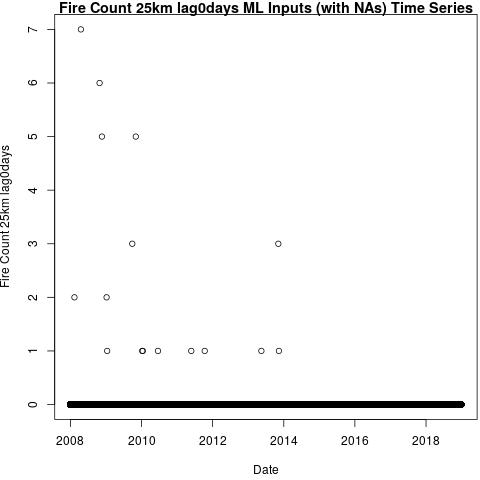
\includegraphics[width=0.77\textwidth]{Code_Outputs/Report_ML_input_PM25_Step4_part_e_de_duplicated_aves_compiled_2019-05-21wNAs_Fire_Count_25km_lag0daysvDate.jpg} 
\caption{\label{fig:Report_ML_input_PM25_Step4_part_e_de_duplicated_aves_compiled_2019-05-21wNAsFire_Count_25km_lag0daysvDate}ML Inputs (with NAs) Time Series} 
\end{figure} 
 

\begin{figure} 
\centering  
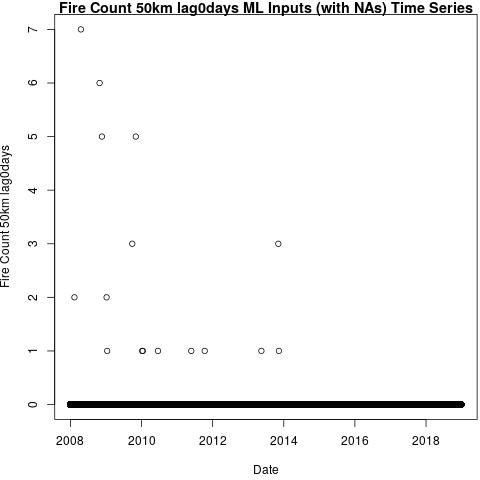
\includegraphics[width=0.77\textwidth]{Code_Outputs/Report_ML_input_PM25_Step4_part_e_de_duplicated_aves_compiled_2019-05-21wNAs_Fire_Count_50km_lag0daysvDate.jpg} 
\caption{\label{fig:Report_ML_input_PM25_Step4_part_e_de_duplicated_aves_compiled_2019-05-21wNAsFire_Count_50km_lag0daysvDate}ML Inputs (with NAs) Time Series} 
\end{figure} 
 

\clearpage 

\begin{figure} 
\centering  
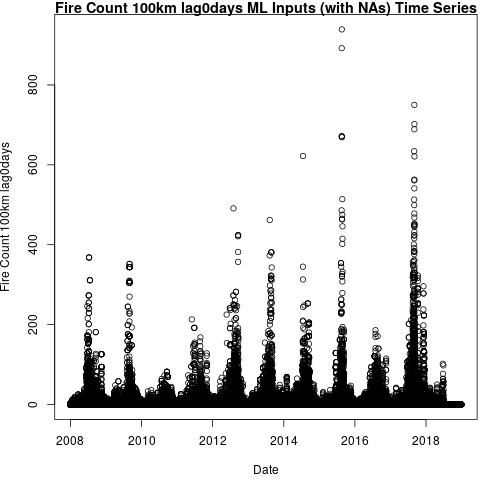
\includegraphics[width=0.77\textwidth]{Code_Outputs/Report_ML_input_PM25_Step4_part_e_de_duplicated_aves_compiled_2019-05-21wNAs_Fire_Count_100km_lag0daysvDate.jpg} 
\caption{\label{fig:Report_ML_input_PM25_Step4_part_e_de_duplicated_aves_compiled_2019-05-21wNAsFire_Count_100km_lag0daysvDate}ML Inputs (with NAs) Time Series} 
\end{figure} 
 

\begin{figure} 
\centering  
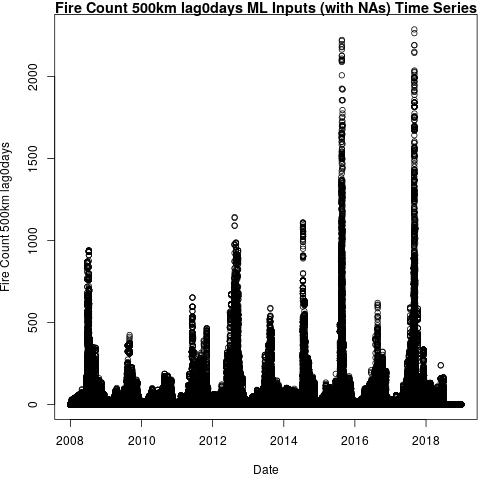
\includegraphics[width=0.77\textwidth]{Code_Outputs/Report_ML_input_PM25_Step4_part_e_de_duplicated_aves_compiled_2019-05-21wNAs_Fire_Count_500km_lag0daysvDate.jpg} 
\caption{\label{fig:Report_ML_input_PM25_Step4_part_e_de_duplicated_aves_compiled_2019-05-21wNAsFire_Count_500km_lag0daysvDate}ML Inputs (with NAs) Time Series} 
\end{figure} 
 

\begin{figure} 
\centering  
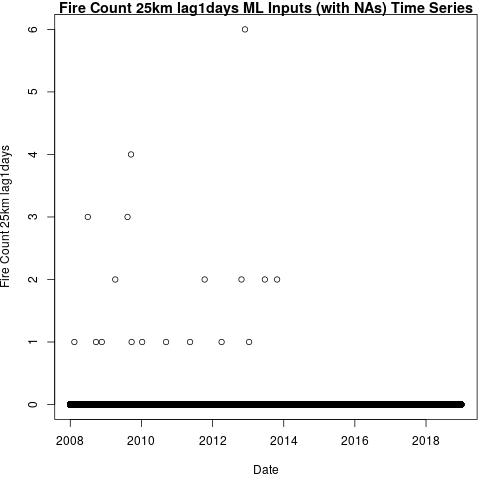
\includegraphics[width=0.77\textwidth]{Code_Outputs/Report_ML_input_PM25_Step4_part_e_de_duplicated_aves_compiled_2019-05-21wNAs_Fire_Count_25km_lag1daysvDate.jpg} 
\caption{\label{fig:Report_ML_input_PM25_Step4_part_e_de_duplicated_aves_compiled_2019-05-21wNAsFire_Count_25km_lag1daysvDate}ML Inputs (with NAs) Time Series} 
\end{figure} 
 

\begin{figure} 
\centering  
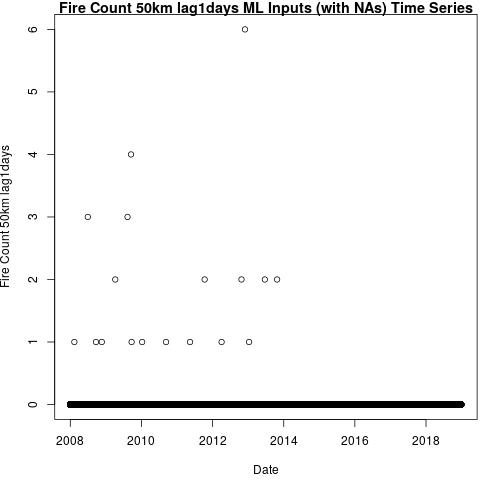
\includegraphics[width=0.77\textwidth]{Code_Outputs/Report_ML_input_PM25_Step4_part_e_de_duplicated_aves_compiled_2019-05-21wNAs_Fire_Count_50km_lag1daysvDate.jpg} 
\caption{\label{fig:Report_ML_input_PM25_Step4_part_e_de_duplicated_aves_compiled_2019-05-21wNAsFire_Count_50km_lag1daysvDate}ML Inputs (with NAs) Time Series} 
\end{figure} 
 

\begin{figure} 
\centering  
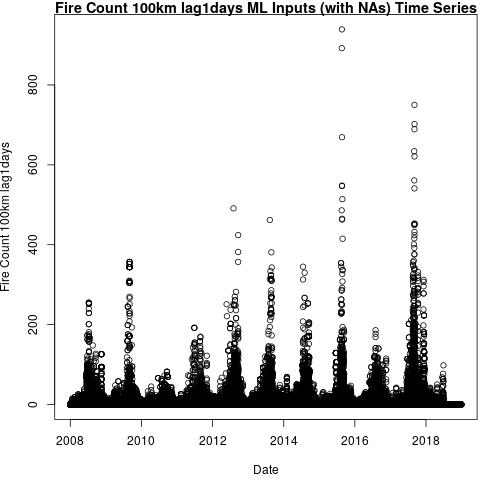
\includegraphics[width=0.77\textwidth]{Code_Outputs/Report_ML_input_PM25_Step4_part_e_de_duplicated_aves_compiled_2019-05-21wNAs_Fire_Count_100km_lag1daysvDate.jpg} 
\caption{\label{fig:Report_ML_input_PM25_Step4_part_e_de_duplicated_aves_compiled_2019-05-21wNAsFire_Count_100km_lag1daysvDate}ML Inputs (with NAs) Time Series} 
\end{figure} 
 

\begin{figure} 
\centering  
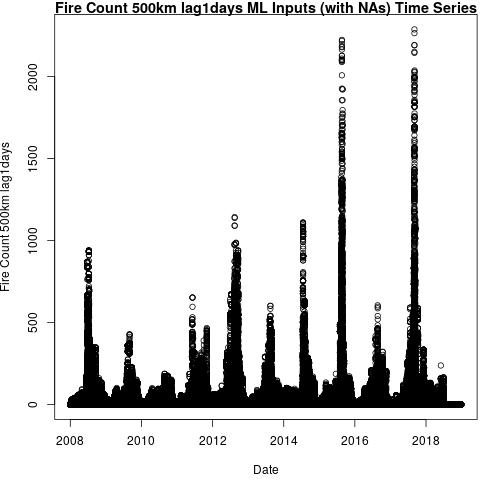
\includegraphics[width=0.77\textwidth]{Code_Outputs/Report_ML_input_PM25_Step4_part_e_de_duplicated_aves_compiled_2019-05-21wNAs_Fire_Count_500km_lag1daysvDate.jpg} 
\caption{\label{fig:Report_ML_input_PM25_Step4_part_e_de_duplicated_aves_compiled_2019-05-21wNAsFire_Count_500km_lag1daysvDate}ML Inputs (with NAs) Time Series} 
\end{figure} 
 

\begin{figure} 
\centering  
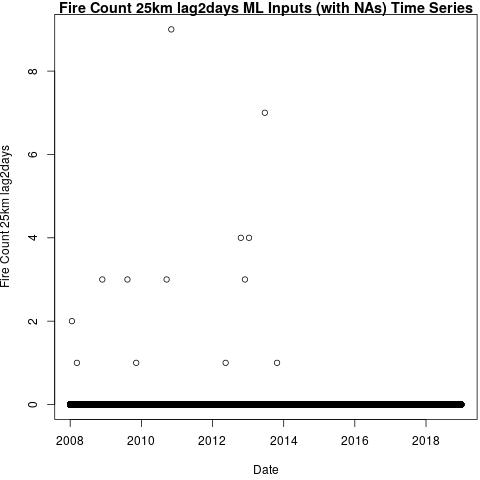
\includegraphics[width=0.77\textwidth]{Code_Outputs/Report_ML_input_PM25_Step4_part_e_de_duplicated_aves_compiled_2019-05-21wNAs_Fire_Count_25km_lag2daysvDate.jpg} 
\caption{\label{fig:Report_ML_input_PM25_Step4_part_e_de_duplicated_aves_compiled_2019-05-21wNAsFire_Count_25km_lag2daysvDate}ML Inputs (with NAs) Time Series} 
\end{figure} 
 

\begin{figure} 
\centering  
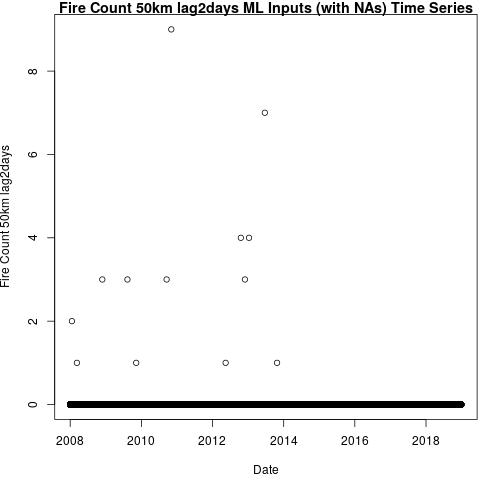
\includegraphics[width=0.77\textwidth]{Code_Outputs/Report_ML_input_PM25_Step4_part_e_de_duplicated_aves_compiled_2019-05-21wNAs_Fire_Count_50km_lag2daysvDate.jpg} 
\caption{\label{fig:Report_ML_input_PM25_Step4_part_e_de_duplicated_aves_compiled_2019-05-21wNAsFire_Count_50km_lag2daysvDate}ML Inputs (with NAs) Time Series} 
\end{figure} 
 

\begin{figure} 
\centering  
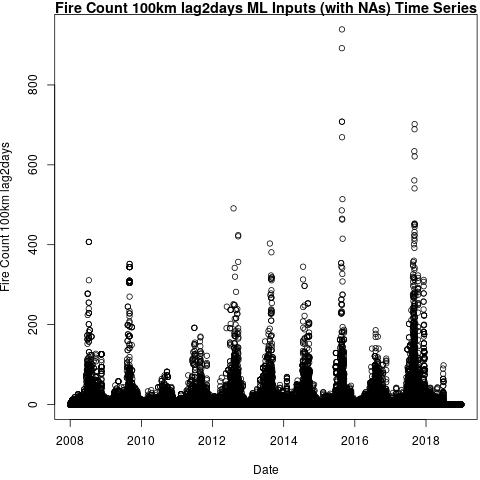
\includegraphics[width=0.77\textwidth]{Code_Outputs/Report_ML_input_PM25_Step4_part_e_de_duplicated_aves_compiled_2019-05-21wNAs_Fire_Count_100km_lag2daysvDate.jpg} 
\caption{\label{fig:Report_ML_input_PM25_Step4_part_e_de_duplicated_aves_compiled_2019-05-21wNAsFire_Count_100km_lag2daysvDate}ML Inputs (with NAs) Time Series} 
\end{figure} 
 

\begin{figure} 
\centering  
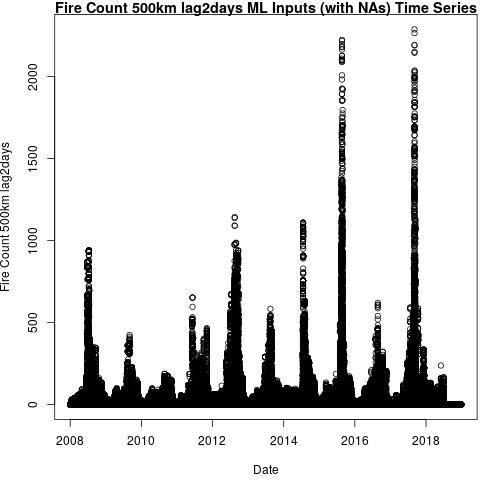
\includegraphics[width=0.77\textwidth]{Code_Outputs/Report_ML_input_PM25_Step4_part_e_de_duplicated_aves_compiled_2019-05-21wNAs_Fire_Count_500km_lag2daysvDate.jpg} 
\caption{\label{fig:Report_ML_input_PM25_Step4_part_e_de_duplicated_aves_compiled_2019-05-21wNAsFire_Count_500km_lag2daysvDate}ML Inputs (with NAs) Time Series} 
\end{figure} 
 

\clearpage 

\begin{figure} 
\centering  
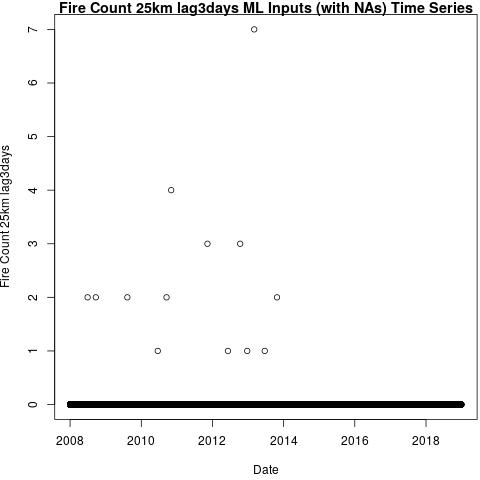
\includegraphics[width=0.77\textwidth]{Code_Outputs/Report_ML_input_PM25_Step4_part_e_de_duplicated_aves_compiled_2019-05-21wNAs_Fire_Count_25km_lag3daysvDate.jpg} 
\caption{\label{fig:Report_ML_input_PM25_Step4_part_e_de_duplicated_aves_compiled_2019-05-21wNAsFire_Count_25km_lag3daysvDate}ML Inputs (with NAs) Time Series} 
\end{figure} 
 

\begin{figure} 
\centering  
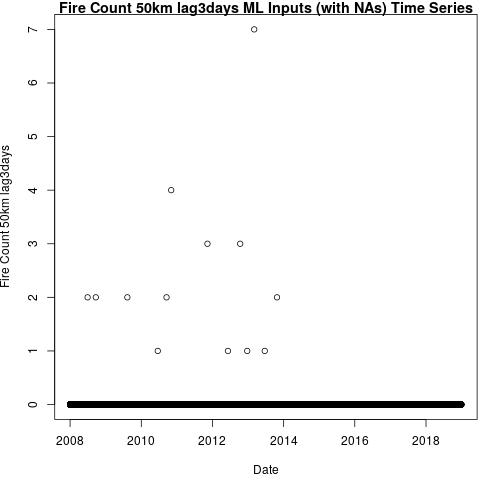
\includegraphics[width=0.77\textwidth]{Code_Outputs/Report_ML_input_PM25_Step4_part_e_de_duplicated_aves_compiled_2019-05-21wNAs_Fire_Count_50km_lag3daysvDate.jpg} 
\caption{\label{fig:Report_ML_input_PM25_Step4_part_e_de_duplicated_aves_compiled_2019-05-21wNAsFire_Count_50km_lag3daysvDate}ML Inputs (with NAs) Time Series} 
\end{figure} 
 

\begin{figure} 
\centering  
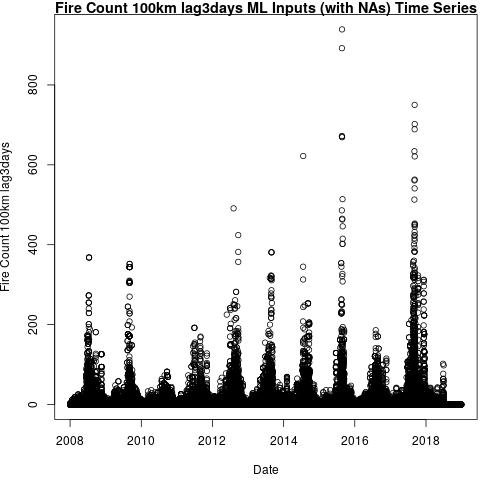
\includegraphics[width=0.77\textwidth]{Code_Outputs/Report_ML_input_PM25_Step4_part_e_de_duplicated_aves_compiled_2019-05-21wNAs_Fire_Count_100km_lag3daysvDate.jpg} 
\caption{\label{fig:Report_ML_input_PM25_Step4_part_e_de_duplicated_aves_compiled_2019-05-21wNAsFire_Count_100km_lag3daysvDate}ML Inputs (with NAs) Time Series} 
\end{figure} 
 

\begin{figure} 
\centering  
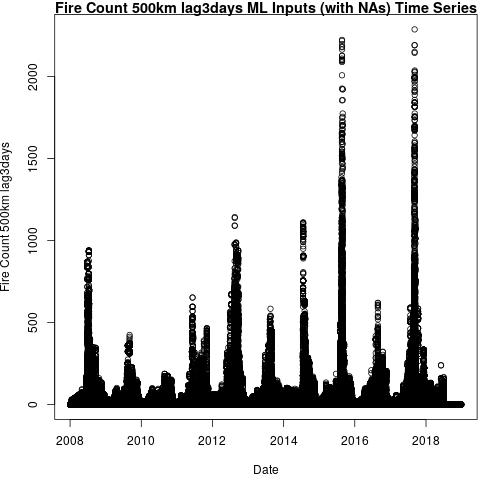
\includegraphics[width=0.77\textwidth]{Code_Outputs/Report_ML_input_PM25_Step4_part_e_de_duplicated_aves_compiled_2019-05-21wNAs_Fire_Count_500km_lag3daysvDate.jpg} 
\caption{\label{fig:Report_ML_input_PM25_Step4_part_e_de_duplicated_aves_compiled_2019-05-21wNAsFire_Count_500km_lag3daysvDate}ML Inputs (with NAs) Time Series} 
\end{figure} 
 

\begin{figure} 
\centering  
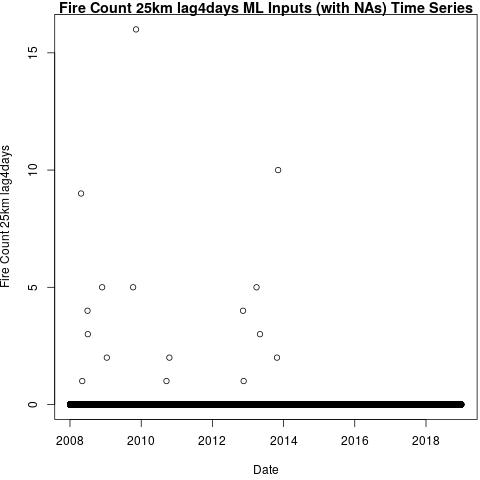
\includegraphics[width=0.77\textwidth]{Code_Outputs/Report_ML_input_PM25_Step4_part_e_de_duplicated_aves_compiled_2019-05-21wNAs_Fire_Count_25km_lag4daysvDate.jpg} 
\caption{\label{fig:Report_ML_input_PM25_Step4_part_e_de_duplicated_aves_compiled_2019-05-21wNAsFire_Count_25km_lag4daysvDate}ML Inputs (with NAs) Time Series} 
\end{figure} 
 

\begin{figure} 
\centering  
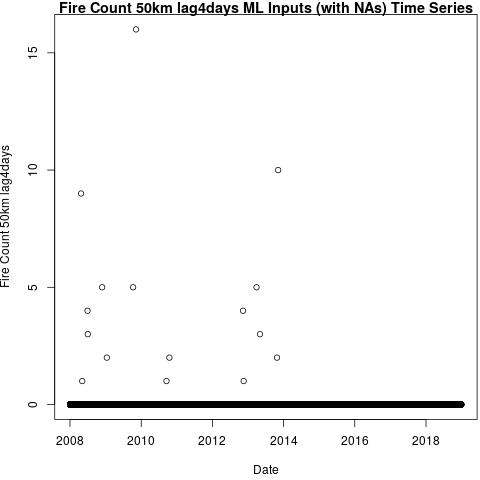
\includegraphics[width=0.77\textwidth]{Code_Outputs/Report_ML_input_PM25_Step4_part_e_de_duplicated_aves_compiled_2019-05-21wNAs_Fire_Count_50km_lag4daysvDate.jpg} 
\caption{\label{fig:Report_ML_input_PM25_Step4_part_e_de_duplicated_aves_compiled_2019-05-21wNAsFire_Count_50km_lag4daysvDate}ML Inputs (with NAs) Time Series} 
\end{figure} 
 

\begin{figure} 
\centering  
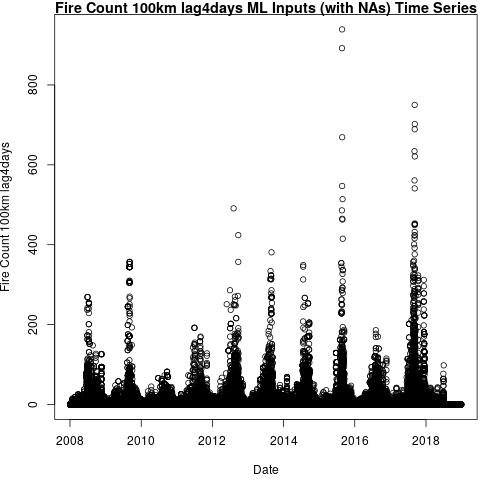
\includegraphics[width=0.77\textwidth]{Code_Outputs/Report_ML_input_PM25_Step4_part_e_de_duplicated_aves_compiled_2019-05-21wNAs_Fire_Count_100km_lag4daysvDate.jpg} 
\caption{\label{fig:Report_ML_input_PM25_Step4_part_e_de_duplicated_aves_compiled_2019-05-21wNAsFire_Count_100km_lag4daysvDate}ML Inputs (with NAs) Time Series} 
\end{figure} 
 

\begin{figure} 
\centering  
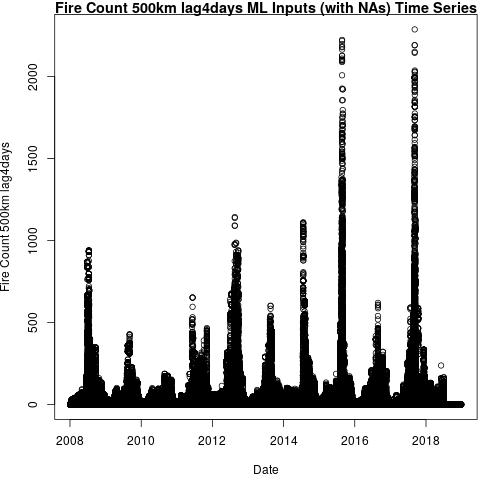
\includegraphics[width=0.77\textwidth]{Code_Outputs/Report_ML_input_PM25_Step4_part_e_de_duplicated_aves_compiled_2019-05-21wNAs_Fire_Count_500km_lag4daysvDate.jpg} 
\caption{\label{fig:Report_ML_input_PM25_Step4_part_e_de_duplicated_aves_compiled_2019-05-21wNAsFire_Count_500km_lag4daysvDate}ML Inputs (with NAs) Time Series} 
\end{figure} 
 

\begin{figure} 
\centering  
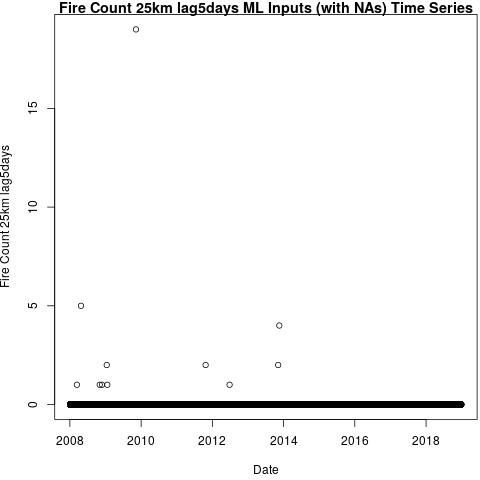
\includegraphics[width=0.77\textwidth]{Code_Outputs/Report_ML_input_PM25_Step4_part_e_de_duplicated_aves_compiled_2019-05-21wNAs_Fire_Count_25km_lag5daysvDate.jpg} 
\caption{\label{fig:Report_ML_input_PM25_Step4_part_e_de_duplicated_aves_compiled_2019-05-21wNAsFire_Count_25km_lag5daysvDate}ML Inputs (with NAs) Time Series} 
\end{figure} 
 

\begin{figure} 
\centering  
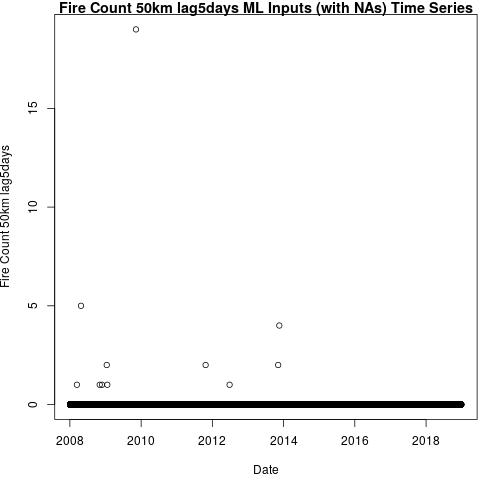
\includegraphics[width=0.77\textwidth]{Code_Outputs/Report_ML_input_PM25_Step4_part_e_de_duplicated_aves_compiled_2019-05-21wNAs_Fire_Count_50km_lag5daysvDate.jpg} 
\caption{\label{fig:Report_ML_input_PM25_Step4_part_e_de_duplicated_aves_compiled_2019-05-21wNAsFire_Count_50km_lag5daysvDate}ML Inputs (with NAs) Time Series} 
\end{figure} 
 

\clearpage 

\begin{figure} 
\centering  
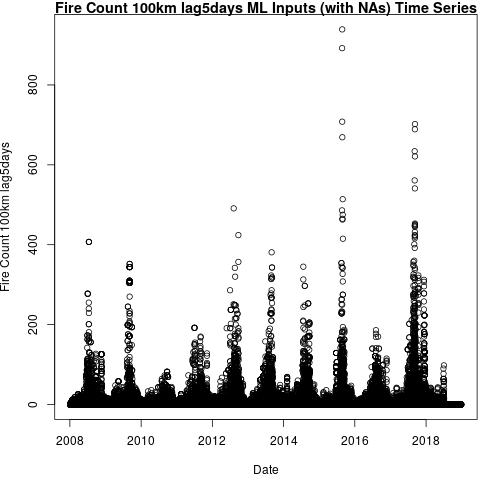
\includegraphics[width=0.77\textwidth]{Code_Outputs/Report_ML_input_PM25_Step4_part_e_de_duplicated_aves_compiled_2019-05-21wNAs_Fire_Count_100km_lag5daysvDate.jpg} 
\caption{\label{fig:Report_ML_input_PM25_Step4_part_e_de_duplicated_aves_compiled_2019-05-21wNAsFire_Count_100km_lag5daysvDate}ML Inputs (with NAs) Time Series} 
\end{figure} 
 

\begin{figure} 
\centering  
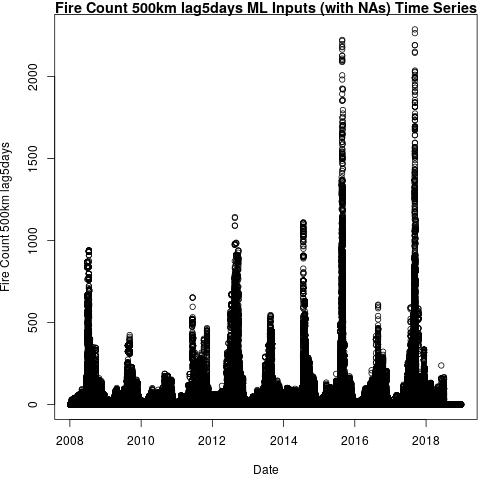
\includegraphics[width=0.77\textwidth]{Code_Outputs/Report_ML_input_PM25_Step4_part_e_de_duplicated_aves_compiled_2019-05-21wNAs_Fire_Count_500km_lag5daysvDate.jpg} 
\caption{\label{fig:Report_ML_input_PM25_Step4_part_e_de_duplicated_aves_compiled_2019-05-21wNAsFire_Count_500km_lag5daysvDate}ML Inputs (with NAs) Time Series} 
\end{figure} 
 

\begin{figure} 
\centering  
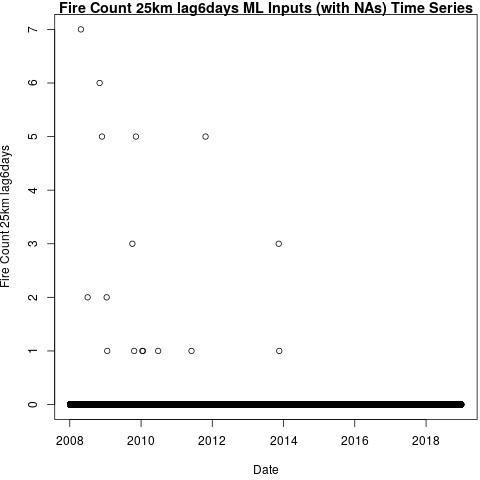
\includegraphics[width=0.77\textwidth]{Code_Outputs/Report_ML_input_PM25_Step4_part_e_de_duplicated_aves_compiled_2019-05-21wNAs_Fire_Count_25km_lag6daysvDate.jpg} 
\caption{\label{fig:Report_ML_input_PM25_Step4_part_e_de_duplicated_aves_compiled_2019-05-21wNAsFire_Count_25km_lag6daysvDate}ML Inputs (with NAs) Time Series} 
\end{figure} 
 

\begin{figure} 
\centering  
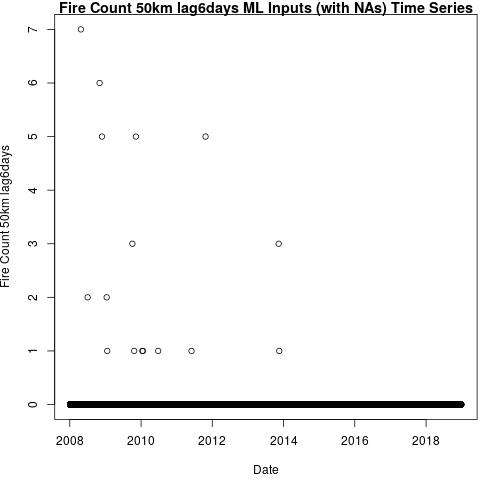
\includegraphics[width=0.77\textwidth]{Code_Outputs/Report_ML_input_PM25_Step4_part_e_de_duplicated_aves_compiled_2019-05-21wNAs_Fire_Count_50km_lag6daysvDate.jpg} 
\caption{\label{fig:Report_ML_input_PM25_Step4_part_e_de_duplicated_aves_compiled_2019-05-21wNAsFire_Count_50km_lag6daysvDate}ML Inputs (with NAs) Time Series} 
\end{figure} 
 

\begin{figure} 
\centering  
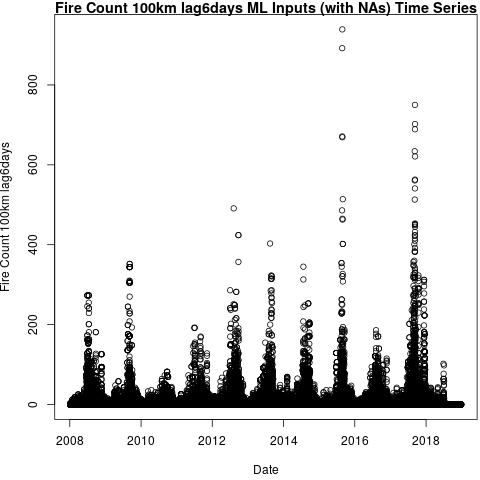
\includegraphics[width=0.77\textwidth]{Code_Outputs/Report_ML_input_PM25_Step4_part_e_de_duplicated_aves_compiled_2019-05-21wNAs_Fire_Count_100km_lag6daysvDate.jpg} 
\caption{\label{fig:Report_ML_input_PM25_Step4_part_e_de_duplicated_aves_compiled_2019-05-21wNAsFire_Count_100km_lag6daysvDate}ML Inputs (with NAs) Time Series} 
\end{figure} 
 

\begin{figure} 
\centering  
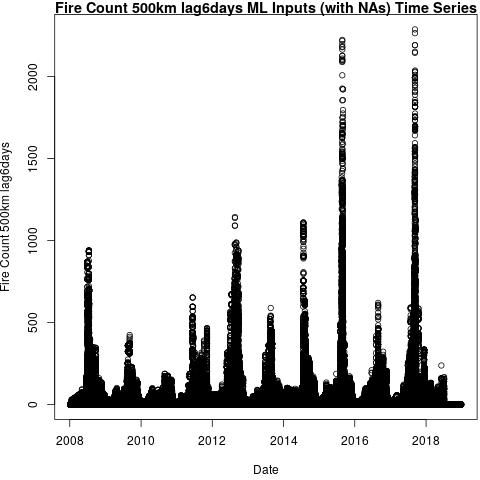
\includegraphics[width=0.77\textwidth]{Code_Outputs/Report_ML_input_PM25_Step4_part_e_de_duplicated_aves_compiled_2019-05-21wNAs_Fire_Count_500km_lag6daysvDate.jpg} 
\caption{\label{fig:Report_ML_input_PM25_Step4_part_e_de_duplicated_aves_compiled_2019-05-21wNAsFire_Count_500km_lag6daysvDate}ML Inputs (with NAs) Time Series} 
\end{figure} 
 

\begin{figure} 
\centering  
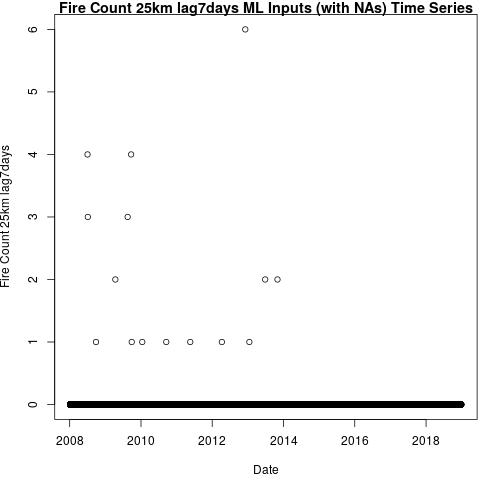
\includegraphics[width=0.77\textwidth]{Code_Outputs/Report_ML_input_PM25_Step4_part_e_de_duplicated_aves_compiled_2019-05-21wNAs_Fire_Count_25km_lag7daysvDate.jpg} 
\caption{\label{fig:Report_ML_input_PM25_Step4_part_e_de_duplicated_aves_compiled_2019-05-21wNAsFire_Count_25km_lag7daysvDate}ML Inputs (with NAs) Time Series} 
\end{figure} 
 

\begin{figure} 
\centering  
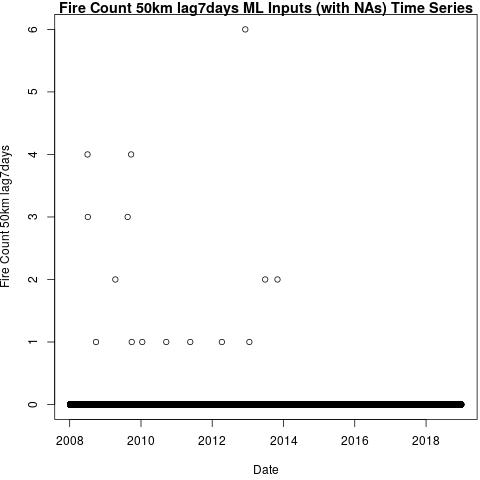
\includegraphics[width=0.77\textwidth]{Code_Outputs/Report_ML_input_PM25_Step4_part_e_de_duplicated_aves_compiled_2019-05-21wNAs_Fire_Count_50km_lag7daysvDate.jpg} 
\caption{\label{fig:Report_ML_input_PM25_Step4_part_e_de_duplicated_aves_compiled_2019-05-21wNAsFire_Count_50km_lag7daysvDate}ML Inputs (with NAs) Time Series} 
\end{figure} 
 

\begin{figure} 
\centering  
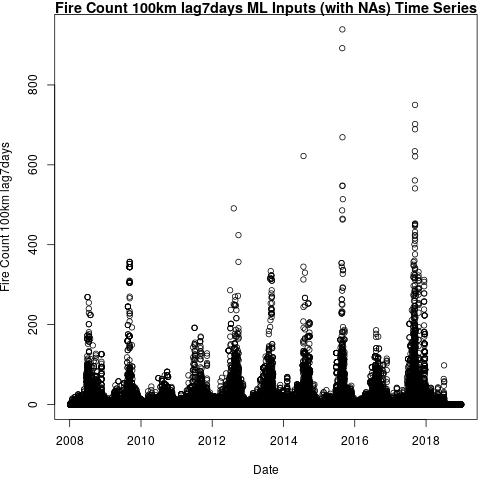
\includegraphics[width=0.77\textwidth]{Code_Outputs/Report_ML_input_PM25_Step4_part_e_de_duplicated_aves_compiled_2019-05-21wNAs_Fire_Count_100km_lag7daysvDate.jpg} 
\caption{\label{fig:Report_ML_input_PM25_Step4_part_e_de_duplicated_aves_compiled_2019-05-21wNAsFire_Count_100km_lag7daysvDate}ML Inputs (with NAs) Time Series} 
\end{figure} 
 

\begin{figure} 
\centering  
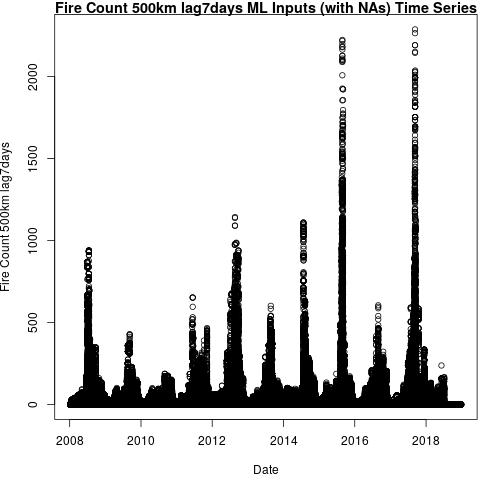
\includegraphics[width=0.77\textwidth]{Code_Outputs/Report_ML_input_PM25_Step4_part_e_de_duplicated_aves_compiled_2019-05-21wNAs_Fire_Count_500km_lag7daysvDate.jpg} 
\caption{\label{fig:Report_ML_input_PM25_Step4_part_e_de_duplicated_aves_compiled_2019-05-21wNAsFire_Count_500km_lag7daysvDate}ML Inputs (with NAs) Time Series} 
\end{figure} 
 

\clearpage 

\begin{figure} 
\centering  
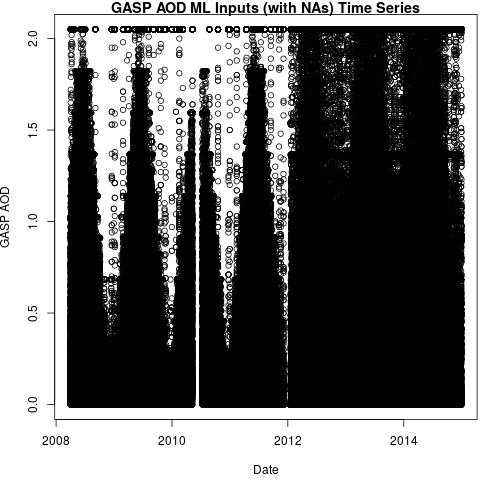
\includegraphics[width=0.77\textwidth]{Code_Outputs/Report_ML_input_PM25_Step4_part_e_de_duplicated_aves_compiled_2019-05-21wNAs_GASP_AODvDate.jpg} 
\caption{\label{fig:Report_ML_input_PM25_Step4_part_e_de_duplicated_aves_compiled_2019-05-21wNAsGASP_AODvDate}ML Inputs (with NAs) Time Series} 
\end{figure} 
 

\begin{figure} 
\centering  
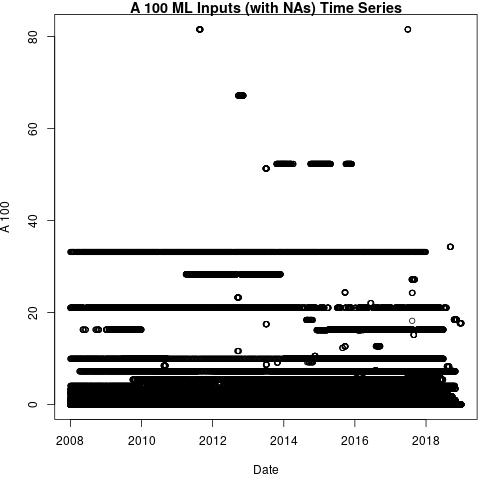
\includegraphics[width=0.77\textwidth]{Code_Outputs/Report_ML_input_PM25_Step4_part_e_de_duplicated_aves_compiled_2019-05-21wNAs_A_100vDate.jpg} 
\caption{\label{fig:Report_ML_input_PM25_Step4_part_e_de_duplicated_aves_compiled_2019-05-21wNAsA_100vDate}ML Inputs (with NAs) Time Series} 
\end{figure} 
 

\begin{figure} 
\centering  
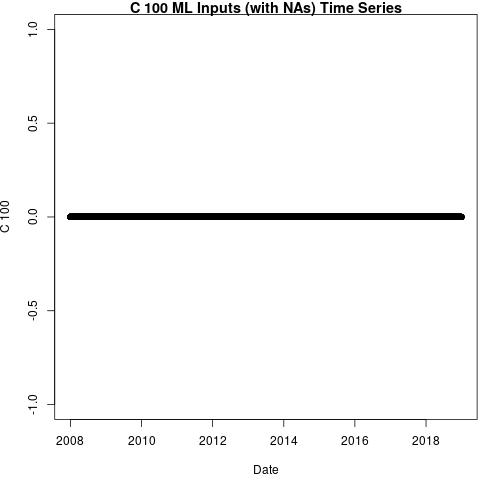
\includegraphics[width=0.77\textwidth]{Code_Outputs/Report_ML_input_PM25_Step4_part_e_de_duplicated_aves_compiled_2019-05-21wNAs_C_100vDate.jpg} 
\caption{\label{fig:Report_ML_input_PM25_Step4_part_e_de_duplicated_aves_compiled_2019-05-21wNAsC_100vDate}ML Inputs (with NAs) Time Series} 
\end{figure} 
 

\begin{figure} 
\centering  
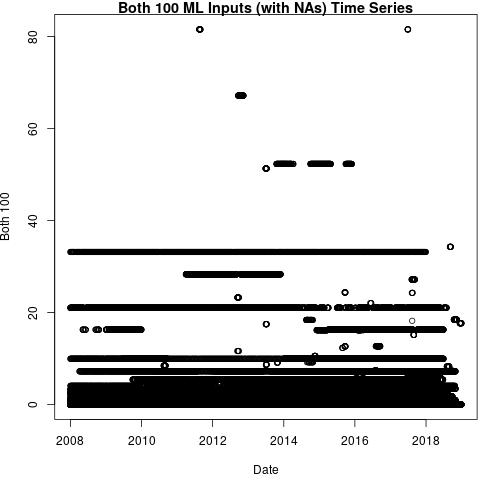
\includegraphics[width=0.77\textwidth]{Code_Outputs/Report_ML_input_PM25_Step4_part_e_de_duplicated_aves_compiled_2019-05-21wNAs_Both_100vDate.jpg} 
\caption{\label{fig:Report_ML_input_PM25_Step4_part_e_de_duplicated_aves_compiled_2019-05-21wNAsBoth_100vDate}ML Inputs (with NAs) Time Series} 
\end{figure} 
 

\begin{figure} 
\centering  
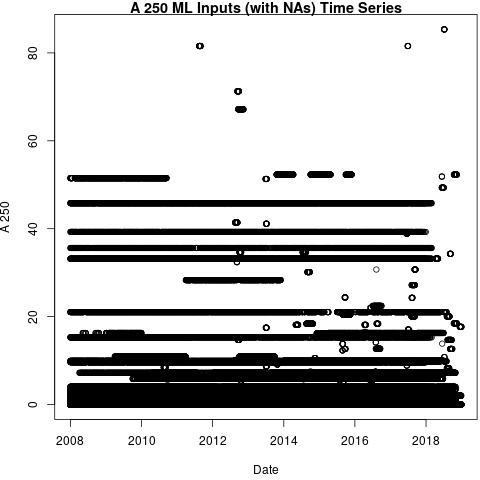
\includegraphics[width=0.77\textwidth]{Code_Outputs/Report_ML_input_PM25_Step4_part_e_de_duplicated_aves_compiled_2019-05-21wNAs_A_250vDate.jpg} 
\caption{\label{fig:Report_ML_input_PM25_Step4_part_e_de_duplicated_aves_compiled_2019-05-21wNAsA_250vDate}ML Inputs (with NAs) Time Series} 
\end{figure} 
 

\begin{figure} 
\centering  
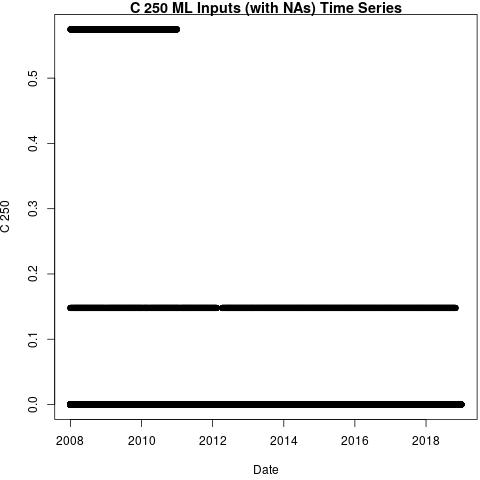
\includegraphics[width=0.77\textwidth]{Code_Outputs/Report_ML_input_PM25_Step4_part_e_de_duplicated_aves_compiled_2019-05-21wNAs_C_250vDate.jpg} 
\caption{\label{fig:Report_ML_input_PM25_Step4_part_e_de_duplicated_aves_compiled_2019-05-21wNAsC_250vDate}ML Inputs (with NAs) Time Series} 
\end{figure} 
 

\begin{figure} 
\centering  
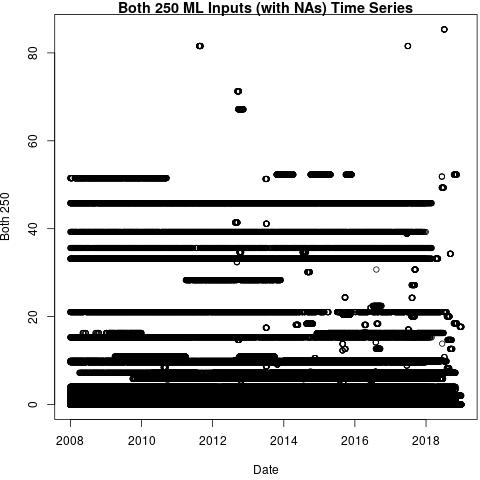
\includegraphics[width=0.77\textwidth]{Code_Outputs/Report_ML_input_PM25_Step4_part_e_de_duplicated_aves_compiled_2019-05-21wNAs_Both_250vDate.jpg} 
\caption{\label{fig:Report_ML_input_PM25_Step4_part_e_de_duplicated_aves_compiled_2019-05-21wNAsBoth_250vDate}ML Inputs (with NAs) Time Series} 
\end{figure} 
 

\begin{figure} 
\centering  
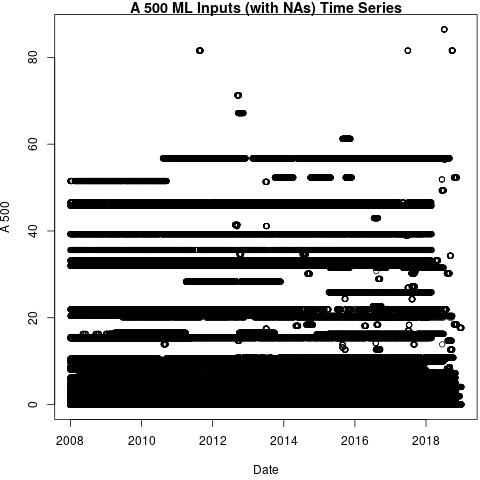
\includegraphics[width=0.77\textwidth]{Code_Outputs/Report_ML_input_PM25_Step4_part_e_de_duplicated_aves_compiled_2019-05-21wNAs_A_500vDate.jpg} 
\caption{\label{fig:Report_ML_input_PM25_Step4_part_e_de_duplicated_aves_compiled_2019-05-21wNAsA_500vDate}ML Inputs (with NAs) Time Series} 
\end{figure} 
 

\begin{figure} 
\centering  
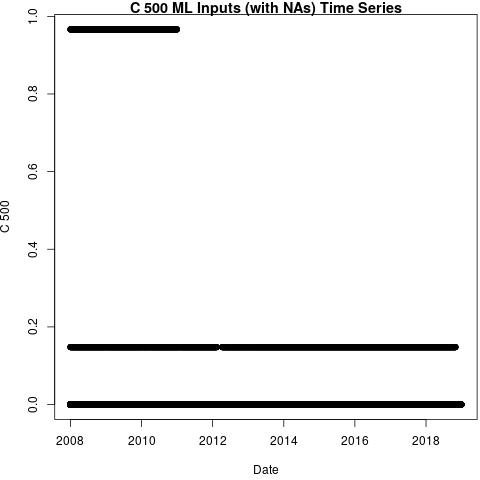
\includegraphics[width=0.77\textwidth]{Code_Outputs/Report_ML_input_PM25_Step4_part_e_de_duplicated_aves_compiled_2019-05-21wNAs_C_500vDate.jpg} 
\caption{\label{fig:Report_ML_input_PM25_Step4_part_e_de_duplicated_aves_compiled_2019-05-21wNAsC_500vDate}ML Inputs (with NAs) Time Series} 
\end{figure} 
 

\begin{figure} 
\centering  
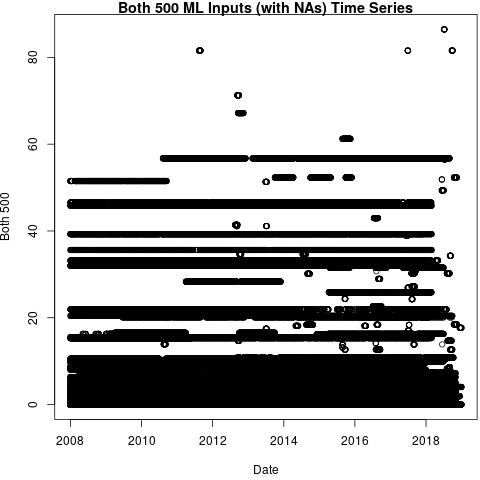
\includegraphics[width=0.77\textwidth]{Code_Outputs/Report_ML_input_PM25_Step4_part_e_de_duplicated_aves_compiled_2019-05-21wNAs_Both_500vDate.jpg} 
\caption{\label{fig:Report_ML_input_PM25_Step4_part_e_de_duplicated_aves_compiled_2019-05-21wNAsBoth_500vDate}ML Inputs (with NAs) Time Series} 
\end{figure} 
 

\clearpage 

\begin{figure} 
\centering  
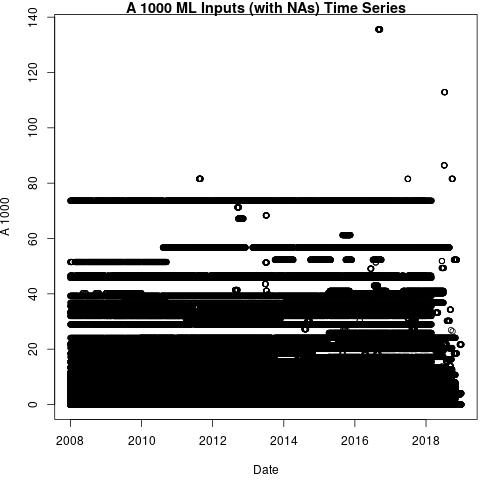
\includegraphics[width=0.77\textwidth]{Code_Outputs/Report_ML_input_PM25_Step4_part_e_de_duplicated_aves_compiled_2019-05-21wNAs_A_1000vDate.jpg} 
\caption{\label{fig:Report_ML_input_PM25_Step4_part_e_de_duplicated_aves_compiled_2019-05-21wNAsA_1000vDate}ML Inputs (with NAs) Time Series} 
\end{figure} 
 

\begin{figure} 
\centering  
\includegraphics[width=0.77\textwidth]{Code_Outputs/Report_ML_input_PM25_Step4_part_e_de_duplicated_aves_compiled_2019-05-21wNAs_Both_1000vDate.jpg} 
\caption{\label{fig:Report_ML_input_PM25_Step4_part_e_de_duplicated_aves_compiled_2019-05-21wNAsBoth_1000vDate}ML Inputs (with NAs) Time Series} 
\end{figure} 
 

\begin{figure} 
\centering  
\includegraphics[width=0.77\textwidth]{Code_Outputs/Report_ML_input_PM25_Step4_part_e_de_duplicated_aves_compiled_2019-05-21wNAs_elevationvDate.jpg} 
\caption{\label{fig:Report_ML_input_PM25_Step4_part_e_de_duplicated_aves_compiled_2019-05-21wNAselevationvDate}ML Inputs (with NAs) Time Series} 
\end{figure} 
 

\begin{figure} 
\centering  
\includegraphics[width=0.77\textwidth]{Code_Outputs/Report_ML_input_PM25_Step4_part_e_de_duplicated_aves_compiled_2019-05-21wNAs_HPBLsurfacevDate.jpg} 
\caption{\label{fig:Report_ML_input_PM25_Step4_part_e_de_duplicated_aves_compiled_2019-05-21wNAsHPBLsurfacevDate}ML Inputs (with NAs) Time Series} 
\end{figure} 
 

\begin{figure} 
\centering  
\includegraphics[width=0.77\textwidth]{Code_Outputs/Report_ML_input_PM25_Step4_part_e_de_duplicated_aves_compiled_2019-05-21wNAs_TMP2mabovegroundvDate.jpg} 
\caption{\label{fig:Report_ML_input_PM25_Step4_part_e_de_duplicated_aves_compiled_2019-05-21wNAsTMP2mabovegroundvDate}ML Inputs (with NAs) Time Series} 
\end{figure} 
 

\begin{figure} 
\centering  
\includegraphics[width=0.77\textwidth]{Code_Outputs/Report_ML_input_PM25_Step4_part_e_de_duplicated_aves_compiled_2019-05-21wNAs_RH2mabovegroundvDate.jpg} 
\caption{\label{fig:Report_ML_input_PM25_Step4_part_e_de_duplicated_aves_compiled_2019-05-21wNAsRH2mabovegroundvDate}ML Inputs (with NAs) Time Series} 
\end{figure} 
 

\begin{figure} 
\centering  
\includegraphics[width=0.77\textwidth]{Code_Outputs/Report_ML_input_PM25_Step4_part_e_de_duplicated_aves_compiled_2019-05-21wNAs_DPT2mabovegroundvDate.jpg} 
\caption{\label{fig:Report_ML_input_PM25_Step4_part_e_de_duplicated_aves_compiled_2019-05-21wNAsDPT2mabovegroundvDate}ML Inputs (with NAs) Time Series} 
\end{figure} 
 

\begin{figure} 
\centering  
\includegraphics[width=0.77\textwidth]{Code_Outputs/Report_ML_input_PM25_Step4_part_e_de_duplicated_aves_compiled_2019-05-21wNAs_APCPsurfacevDate.jpg} 
\caption{\label{fig:Report_ML_input_PM25_Step4_part_e_de_duplicated_aves_compiled_2019-05-21wNAsAPCPsurfacevDate}ML Inputs (with NAs) Time Series} 
\end{figure} 
 

\begin{figure} 
\centering  
\includegraphics[width=0.77\textwidth]{Code_Outputs/Report_ML_input_PM25_Step4_part_e_de_duplicated_aves_compiled_2019-05-21wNAs_WEASDsurfacevDate.jpg} 
\caption{\label{fig:Report_ML_input_PM25_Step4_part_e_de_duplicated_aves_compiled_2019-05-21wNAsWEASDsurfacevDate}ML Inputs (with NAs) Time Series} 
\end{figure} 
 

\begin{figure} 
\centering  
\includegraphics[width=0.77\textwidth]{Code_Outputs/Report_ML_input_PM25_Step4_part_e_de_duplicated_aves_compiled_2019-05-21wNAs_SNOWCsurfacevDate.jpg} 
\caption{\label{fig:Report_ML_input_PM25_Step4_part_e_de_duplicated_aves_compiled_2019-05-21wNAsSNOWCsurfacevDate}ML Inputs (with NAs) Time Series} 
\end{figure} 
 

\clearpage 

\begin{figure} 
\centering  
\includegraphics[width=0.77\textwidth]{Code_Outputs/Report_ML_input_PM25_Step4_part_e_de_duplicated_aves_compiled_2019-05-21wNAs_UGRD10mabovegroundvDate.jpg} 
\caption{\label{fig:Report_ML_input_PM25_Step4_part_e_de_duplicated_aves_compiled_2019-05-21wNAsUGRD10mabovegroundvDate}ML Inputs (with NAs) Time Series} 
\end{figure} 
 

\begin{figure} 
\centering  
\includegraphics[width=0.77\textwidth]{Code_Outputs/Report_ML_input_PM25_Step4_part_e_de_duplicated_aves_compiled_2019-05-21wNAs_VGRD10mabovegroundvDate.jpg} 
\caption{\label{fig:Report_ML_input_PM25_Step4_part_e_de_duplicated_aves_compiled_2019-05-21wNAsVGRD10mabovegroundvDate}ML Inputs (with NAs) Time Series} 
\end{figure} 
 

\begin{figure} 
\centering  
\includegraphics[width=0.77\textwidth]{Code_Outputs/Report_ML_input_PM25_Step4_part_e_de_duplicated_aves_compiled_2019-05-21wNAs_PRMSLmeansealevelvDate.jpg} 
\caption{\label{fig:Report_ML_input_PM25_Step4_part_e_de_duplicated_aves_compiled_2019-05-21wNAsPRMSLmeansealevelvDate}ML Inputs (with NAs) Time Series} 
\end{figure} 
 

\begin{figure} 
\centering  
\includegraphics[width=0.77\textwidth]{Code_Outputs/Report_ML_input_PM25_Step4_part_e_de_duplicated_aves_compiled_2019-05-21wNAs_PRESsurfacevDate.jpg} 
\caption{\label{fig:Report_ML_input_PM25_Step4_part_e_de_duplicated_aves_compiled_2019-05-21wNAsPRESsurfacevDate}ML Inputs (with NAs) Time Series} 
\end{figure} 
 

\begin{figure} 
\centering  
\includegraphics[width=0.77\textwidth]{Code_Outputs/Report_ML_input_PM25_Step4_part_e_de_duplicated_aves_compiled_2019-05-21wNAs_DZDT850mbvDate.jpg} 
\caption{\label{fig:Report_ML_input_PM25_Step4_part_e_de_duplicated_aves_compiled_2019-05-21wNAsDZDT850mbvDate}ML Inputs (with NAs) Time Series} 
\end{figure} 
 

\begin{figure} 
\centering  
\includegraphics[width=0.77\textwidth]{Code_Outputs/Report_ML_input_PM25_Step4_part_e_de_duplicated_aves_compiled_2019-05-21wNAs_DZDT700mbvDate.jpg} 
\caption{\label{fig:Report_ML_input_PM25_Step4_part_e_de_duplicated_aves_compiled_2019-05-21wNAsDZDT700mbvDate}ML Inputs (with NAs) Time Series} 
\end{figure} 
 

\begin{figure} 
\centering  
\includegraphics[width=0.77\textwidth]{Code_Outputs/Report_ML_input_PM25_Step4_part_e_de_duplicated_aves_compiled_2019-05-21wNAs_NLCD_1km_percent_urban_buffervDate.jpg} 
\caption{\label{fig:Report_ML_input_PM25_Step4_part_e_de_duplicated_aves_compiled_2019-05-21wNAsNLCD_1km_percent_urban_buffervDate}ML Inputs (with NAs) Time Series} 
\end{figure} 
 

\begin{figure} 
\centering  
\includegraphics[width=0.77\textwidth]{Code_Outputs/Report_ML_input_PM25_Step4_part_e_de_duplicated_aves_compiled_2019-05-21wNAs_NLCD_5km_percent_urban_buffervDate.jpg} 
\caption{\label{fig:Report_ML_input_PM25_Step4_part_e_de_duplicated_aves_compiled_2019-05-21wNAsNLCD_5km_percent_urban_buffervDate}ML Inputs (with NAs) Time Series} 
\end{figure} 
 

\begin{figure} 
\centering  
\includegraphics[width=0.77\textwidth]{Code_Outputs/Report_ML_input_PM25_Step4_part_e_de_duplicated_aves_compiled_2019-05-21wNAs_NLCD_10km_percent_urban_buffervDate.jpg} 
\caption{\label{fig:Report_ML_input_PM25_Step4_part_e_de_duplicated_aves_compiled_2019-05-21wNAsNLCD_10km_percent_urban_buffervDate}ML Inputs (with NAs) Time Series} 
\end{figure} 
 

\begin{figure} 
\centering  
\includegraphics[width=0.77\textwidth]{Code_Outputs/Report_ML_input_PM25_Step4_part_e_de_duplicated_aves_compiled_2019-05-21wNAs_ndvivDate.jpg} 
\caption{\label{fig:Report_ML_input_PM25_Step4_part_e_de_duplicated_aves_compiled_2019-05-21wNAsndvivDate}ML Inputs (with NAs) Time Series} 
\end{figure} 
 

\clearpage 

\begin{figure} 
\centering  
\includegraphics[width=0.77\textwidth]{Code_Outputs/Report_ML_input_PM25_Step4_part_e_de_duplicated_aves_compiled_2019-05-21wNAs_DayOfWeekvDate.jpg} 
\caption{\label{fig:Report_ML_input_PM25_Step4_part_e_de_duplicated_aves_compiled_2019-05-21wNAsDayOfWeekvDate}ML Inputs (with NAs) Time Series} 
\end{figure} 
 

\begin{figure} 
\centering  
\includegraphics[width=0.77\textwidth]{Code_Outputs/Report_ML_input_PM25_Step4_part_e_de_duplicated_aves_compiled_2019-05-21wNAs_WintervDate.jpg} 
\caption{\label{fig:Report_ML_input_PM25_Step4_part_e_de_duplicated_aves_compiled_2019-05-21wNAsWintervDate}ML Inputs (with NAs) Time Series} 
\end{figure} 
 

\begin{figure} 
\centering  
\includegraphics[width=0.77\textwidth]{Code_Outputs/Report_ML_input_PM25_Step4_part_e_de_duplicated_aves_compiled_2019-05-21wNAs_SpringvDate.jpg} 
\caption{\label{fig:Report_ML_input_PM25_Step4_part_e_de_duplicated_aves_compiled_2019-05-21wNAsSpringvDate}ML Inputs (with NAs) Time Series} 
\end{figure} 
 

\begin{figure} 
\centering  
\includegraphics[width=0.77\textwidth]{Code_Outputs/Report_ML_input_PM25_Step4_part_e_de_duplicated_aves_compiled_2019-05-21wNAs_SummervDate.jpg} 
\caption{\label{fig:Report_ML_input_PM25_Step4_part_e_de_duplicated_aves_compiled_2019-05-21wNAsSummervDate}ML Inputs (with NAs) Time Series} 
\end{figure} 
 

\begin{figure} 
\centering  
\includegraphics[width=0.77\textwidth]{Code_Outputs/Report_ML_input_PM25_Step4_part_e_de_duplicated_aves_compiled_2019-05-21wNAs_FallvDate.jpg} 
\caption{\label{fig:Report_ML_input_PM25_Step4_part_e_de_duplicated_aves_compiled_2019-05-21wNAsFallvDate}ML Inputs (with NAs) Time Series} 
\end{figure} 
 
 

% PM2.5 vs predictor for each predictor variable 

\subsection{ML Inputs (with NAs) Plot against PM2.5 Obs Images} 
 

\begin{figure} 
\centering  
\includegraphics[width=0.77\textwidth]{Code_Outputs/Report_ML_input_PM25_Step4_part_e_de_duplicated_aves_compiled_2019-05-21wNAs_Fire_Count_25km_lag0daysvPM25_Obs.jpg} 
\caption{\label{fig:Report_ML_input_PM25_Step4_part_e_de_duplicated_aves_compiled_2019-05-21wNAsFire_Count_25km_lag0daysvPM25_Obs}ML Inputs (with NAs) Plot against PM2.5 Obs} 
\end{figure} 
 

\begin{figure} 
\centering  
\includegraphics[width=0.77\textwidth]{Code_Outputs/Report_ML_input_PM25_Step4_part_e_de_duplicated_aves_compiled_2019-05-21wNAs_Fire_Count_50km_lag0daysvPM25_Obs.jpg} 
\caption{\label{fig:Report_ML_input_PM25_Step4_part_e_de_duplicated_aves_compiled_2019-05-21wNAsFire_Count_50km_lag0daysvPM25_Obs}ML Inputs (with NAs) Plot against PM2.5 Obs} 
\end{figure} 
 

\begin{figure} 
\centering  
\includegraphics[width=0.77\textwidth]{Code_Outputs/Report_ML_input_PM25_Step4_part_e_de_duplicated_aves_compiled_2019-05-21wNAs_Fire_Count_100km_lag0daysvPM25_Obs.jpg} 
\caption{\label{fig:Report_ML_input_PM25_Step4_part_e_de_duplicated_aves_compiled_2019-05-21wNAsFire_Count_100km_lag0daysvPM25_Obs}ML Inputs (with NAs) Plot against PM2.5 Obs} 
\end{figure} 
 

\begin{figure} 
\centering  
\includegraphics[width=0.77\textwidth]{Code_Outputs/Report_ML_input_PM25_Step4_part_e_de_duplicated_aves_compiled_2019-05-21wNAs_Fire_Count_500km_lag0daysvPM25_Obs.jpg} 
\caption{\label{fig:Report_ML_input_PM25_Step4_part_e_de_duplicated_aves_compiled_2019-05-21wNAsFire_Count_500km_lag0daysvPM25_Obs}ML Inputs (with NAs) Plot against PM2.5 Obs} 
\end{figure} 
 

\begin{figure} 
\centering  
\includegraphics[width=0.77\textwidth]{Code_Outputs/Report_ML_input_PM25_Step4_part_e_de_duplicated_aves_compiled_2019-05-21wNAs_Fire_Count_25km_lag1daysvPM25_Obs.jpg} 
\caption{\label{fig:Report_ML_input_PM25_Step4_part_e_de_duplicated_aves_compiled_2019-05-21wNAsFire_Count_25km_lag1daysvPM25_Obs}ML Inputs (with NAs) Plot against PM2.5 Obs} 
\end{figure} 
 

\begin{figure} 
\centering  
\includegraphics[width=0.77\textwidth]{Code_Outputs/Report_ML_input_PM25_Step4_part_e_de_duplicated_aves_compiled_2019-05-21wNAs_Fire_Count_50km_lag1daysvPM25_Obs.jpg} 
\caption{\label{fig:Report_ML_input_PM25_Step4_part_e_de_duplicated_aves_compiled_2019-05-21wNAsFire_Count_50km_lag1daysvPM25_Obs}ML Inputs (with NAs) Plot against PM2.5 Obs} 
\end{figure} 
 

\begin{figure} 
\centering  
\includegraphics[width=0.77\textwidth]{Code_Outputs/Report_ML_input_PM25_Step4_part_e_de_duplicated_aves_compiled_2019-05-21wNAs_Fire_Count_100km_lag1daysvPM25_Obs.jpg} 
\caption{\label{fig:Report_ML_input_PM25_Step4_part_e_de_duplicated_aves_compiled_2019-05-21wNAsFire_Count_100km_lag1daysvPM25_Obs}ML Inputs (with NAs) Plot against PM2.5 Obs} 
\end{figure} 
 

\begin{figure} 
\centering  
\includegraphics[width=0.77\textwidth]{Code_Outputs/Report_ML_input_PM25_Step4_part_e_de_duplicated_aves_compiled_2019-05-21wNAs_Fire_Count_500km_lag1daysvPM25_Obs.jpg} 
\caption{\label{fig:Report_ML_input_PM25_Step4_part_e_de_duplicated_aves_compiled_2019-05-21wNAsFire_Count_500km_lag1daysvPM25_Obs}ML Inputs (with NAs) Plot against PM2.5 Obs} 
\end{figure} 
 

\begin{figure} 
\centering  
\includegraphics[width=0.77\textwidth]{Code_Outputs/Report_ML_input_PM25_Step4_part_e_de_duplicated_aves_compiled_2019-05-21wNAs_Fire_Count_25km_lag2daysvPM25_Obs.jpg} 
\caption{\label{fig:Report_ML_input_PM25_Step4_part_e_de_duplicated_aves_compiled_2019-05-21wNAsFire_Count_25km_lag2daysvPM25_Obs}ML Inputs (with NAs) Plot against PM2.5 Obs} 
\end{figure} 
 

\clearpage 

\begin{figure} 
\centering  
\includegraphics[width=0.77\textwidth]{Code_Outputs/Report_ML_input_PM25_Step4_part_e_de_duplicated_aves_compiled_2019-05-21wNAs_Fire_Count_50km_lag2daysvPM25_Obs.jpg} 
\caption{\label{fig:Report_ML_input_PM25_Step4_part_e_de_duplicated_aves_compiled_2019-05-21wNAsFire_Count_50km_lag2daysvPM25_Obs}ML Inputs (with NAs) Plot against PM2.5 Obs} 
\end{figure} 
 

\begin{figure} 
\centering  
\includegraphics[width=0.77\textwidth]{Code_Outputs/Report_ML_input_PM25_Step4_part_e_de_duplicated_aves_compiled_2019-05-21wNAs_Fire_Count_100km_lag2daysvPM25_Obs.jpg} 
\caption{\label{fig:Report_ML_input_PM25_Step4_part_e_de_duplicated_aves_compiled_2019-05-21wNAsFire_Count_100km_lag2daysvPM25_Obs}ML Inputs (with NAs) Plot against PM2.5 Obs} 
\end{figure} 
 

\begin{figure} 
\centering  
\includegraphics[width=0.77\textwidth]{Code_Outputs/Report_ML_input_PM25_Step4_part_e_de_duplicated_aves_compiled_2019-05-21wNAs_Fire_Count_500km_lag2daysvPM25_Obs.jpg} 
\caption{\label{fig:Report_ML_input_PM25_Step4_part_e_de_duplicated_aves_compiled_2019-05-21wNAsFire_Count_500km_lag2daysvPM25_Obs}ML Inputs (with NAs) Plot against PM2.5 Obs} 
\end{figure} 
 

\begin{figure} 
\centering  
\includegraphics[width=0.77\textwidth]{Code_Outputs/Report_ML_input_PM25_Step4_part_e_de_duplicated_aves_compiled_2019-05-21wNAs_Fire_Count_25km_lag3daysvPM25_Obs.jpg} 
\caption{\label{fig:Report_ML_input_PM25_Step4_part_e_de_duplicated_aves_compiled_2019-05-21wNAsFire_Count_25km_lag3daysvPM25_Obs}ML Inputs (with NAs) Plot against PM2.5 Obs} 
\end{figure} 
 

\begin{figure} 
\centering  
\includegraphics[width=0.77\textwidth]{Code_Outputs/Report_ML_input_PM25_Step4_part_e_de_duplicated_aves_compiled_2019-05-21wNAs_Fire_Count_50km_lag3daysvPM25_Obs.jpg} 
\caption{\label{fig:Report_ML_input_PM25_Step4_part_e_de_duplicated_aves_compiled_2019-05-21wNAsFire_Count_50km_lag3daysvPM25_Obs}ML Inputs (with NAs) Plot against PM2.5 Obs} 
\end{figure} 
 

\begin{figure} 
\centering  
\includegraphics[width=0.77\textwidth]{Code_Outputs/Report_ML_input_PM25_Step4_part_e_de_duplicated_aves_compiled_2019-05-21wNAs_Fire_Count_100km_lag3daysvPM25_Obs.jpg} 
\caption{\label{fig:Report_ML_input_PM25_Step4_part_e_de_duplicated_aves_compiled_2019-05-21wNAsFire_Count_100km_lag3daysvPM25_Obs}ML Inputs (with NAs) Plot against PM2.5 Obs} 
\end{figure} 
 

\begin{figure} 
\centering  
\includegraphics[width=0.77\textwidth]{Code_Outputs/Report_ML_input_PM25_Step4_part_e_de_duplicated_aves_compiled_2019-05-21wNAs_Fire_Count_500km_lag3daysvPM25_Obs.jpg} 
\caption{\label{fig:Report_ML_input_PM25_Step4_part_e_de_duplicated_aves_compiled_2019-05-21wNAsFire_Count_500km_lag3daysvPM25_Obs}ML Inputs (with NAs) Plot against PM2.5 Obs} 
\end{figure} 
 

\begin{figure} 
\centering  
\includegraphics[width=0.77\textwidth]{Code_Outputs/Report_ML_input_PM25_Step4_part_e_de_duplicated_aves_compiled_2019-05-21wNAs_Fire_Count_25km_lag4daysvPM25_Obs.jpg} 
\caption{\label{fig:Report_ML_input_PM25_Step4_part_e_de_duplicated_aves_compiled_2019-05-21wNAsFire_Count_25km_lag4daysvPM25_Obs}ML Inputs (with NAs) Plot against PM2.5 Obs} 
\end{figure} 
 

\begin{figure} 
\centering  
\includegraphics[width=0.77\textwidth]{Code_Outputs/Report_ML_input_PM25_Step4_part_e_de_duplicated_aves_compiled_2019-05-21wNAs_Fire_Count_50km_lag4daysvPM25_Obs.jpg} 
\caption{\label{fig:Report_ML_input_PM25_Step4_part_e_de_duplicated_aves_compiled_2019-05-21wNAsFire_Count_50km_lag4daysvPM25_Obs}ML Inputs (with NAs) Plot against PM2.5 Obs} 
\end{figure} 
 

\begin{figure} 
\centering  
\includegraphics[width=0.77\textwidth]{Code_Outputs/Report_ML_input_PM25_Step4_part_e_de_duplicated_aves_compiled_2019-05-21wNAs_Fire_Count_100km_lag4daysvPM25_Obs.jpg} 
\caption{\label{fig:Report_ML_input_PM25_Step4_part_e_de_duplicated_aves_compiled_2019-05-21wNAsFire_Count_100km_lag4daysvPM25_Obs}ML Inputs (with NAs) Plot against PM2.5 Obs} 
\end{figure} 
 

\clearpage 

\begin{figure} 
\centering  
\includegraphics[width=0.77\textwidth]{Code_Outputs/Report_ML_input_PM25_Step4_part_e_de_duplicated_aves_compiled_2019-05-21wNAs_Fire_Count_500km_lag4daysvPM25_Obs.jpg} 
\caption{\label{fig:Report_ML_input_PM25_Step4_part_e_de_duplicated_aves_compiled_2019-05-21wNAsFire_Count_500km_lag4daysvPM25_Obs}ML Inputs (with NAs) Plot against PM2.5 Obs} 
\end{figure} 
 

\begin{figure} 
\centering  
\includegraphics[width=0.77\textwidth]{Code_Outputs/Report_ML_input_PM25_Step4_part_e_de_duplicated_aves_compiled_2019-05-21wNAs_Fire_Count_25km_lag5daysvPM25_Obs.jpg} 
\caption{\label{fig:Report_ML_input_PM25_Step4_part_e_de_duplicated_aves_compiled_2019-05-21wNAsFire_Count_25km_lag5daysvPM25_Obs}ML Inputs (with NAs) Plot against PM2.5 Obs} 
\end{figure} 
 

\begin{figure} 
\centering  
\includegraphics[width=0.77\textwidth]{Code_Outputs/Report_ML_input_PM25_Step4_part_e_de_duplicated_aves_compiled_2019-05-21wNAs_Fire_Count_50km_lag5daysvPM25_Obs.jpg} 
\caption{\label{fig:Report_ML_input_PM25_Step4_part_e_de_duplicated_aves_compiled_2019-05-21wNAsFire_Count_50km_lag5daysvPM25_Obs}ML Inputs (with NAs) Plot against PM2.5 Obs} 
\end{figure} 
 

\begin{figure} 
\centering  
\includegraphics[width=0.77\textwidth]{Code_Outputs/Report_ML_input_PM25_Step4_part_e_de_duplicated_aves_compiled_2019-05-21wNAs_Fire_Count_100km_lag5daysvPM25_Obs.jpg} 
\caption{\label{fig:Report_ML_input_PM25_Step4_part_e_de_duplicated_aves_compiled_2019-05-21wNAsFire_Count_100km_lag5daysvPM25_Obs}ML Inputs (with NAs) Plot against PM2.5 Obs} 
\end{figure} 
 

\begin{figure} 
\centering  
\includegraphics[width=0.77\textwidth]{Code_Outputs/Report_ML_input_PM25_Step4_part_e_de_duplicated_aves_compiled_2019-05-21wNAs_Fire_Count_500km_lag5daysvPM25_Obs.jpg} 
\caption{\label{fig:Report_ML_input_PM25_Step4_part_e_de_duplicated_aves_compiled_2019-05-21wNAsFire_Count_500km_lag5daysvPM25_Obs}ML Inputs (with NAs) Plot against PM2.5 Obs} 
\end{figure} 
 

\begin{figure} 
\centering  
\includegraphics[width=0.77\textwidth]{Code_Outputs/Report_ML_input_PM25_Step4_part_e_de_duplicated_aves_compiled_2019-05-21wNAs_Fire_Count_25km_lag6daysvPM25_Obs.jpg} 
\caption{\label{fig:Report_ML_input_PM25_Step4_part_e_de_duplicated_aves_compiled_2019-05-21wNAsFire_Count_25km_lag6daysvPM25_Obs}ML Inputs (with NAs) Plot against PM2.5 Obs} 
\end{figure} 
 

\begin{figure} 
\centering  
\includegraphics[width=0.77\textwidth]{Code_Outputs/Report_ML_input_PM25_Step4_part_e_de_duplicated_aves_compiled_2019-05-21wNAs_Fire_Count_50km_lag6daysvPM25_Obs.jpg} 
\caption{\label{fig:Report_ML_input_PM25_Step4_part_e_de_duplicated_aves_compiled_2019-05-21wNAsFire_Count_50km_lag6daysvPM25_Obs}ML Inputs (with NAs) Plot against PM2.5 Obs} 
\end{figure} 
 

\begin{figure} 
\centering  
\includegraphics[width=0.77\textwidth]{Code_Outputs/Report_ML_input_PM25_Step4_part_e_de_duplicated_aves_compiled_2019-05-21wNAs_Fire_Count_100km_lag6daysvPM25_Obs.jpg} 
\caption{\label{fig:Report_ML_input_PM25_Step4_part_e_de_duplicated_aves_compiled_2019-05-21wNAsFire_Count_100km_lag6daysvPM25_Obs}ML Inputs (with NAs) Plot against PM2.5 Obs} 
\end{figure} 
 

\begin{figure} 
\centering  
\includegraphics[width=0.77\textwidth]{Code_Outputs/Report_ML_input_PM25_Step4_part_e_de_duplicated_aves_compiled_2019-05-21wNAs_Fire_Count_500km_lag6daysvPM25_Obs.jpg} 
\caption{\label{fig:Report_ML_input_PM25_Step4_part_e_de_duplicated_aves_compiled_2019-05-21wNAsFire_Count_500km_lag6daysvPM25_Obs}ML Inputs (with NAs) Plot against PM2.5 Obs} 
\end{figure} 
 

\begin{figure} 
\centering  
\includegraphics[width=0.77\textwidth]{Code_Outputs/Report_ML_input_PM25_Step4_part_e_de_duplicated_aves_compiled_2019-05-21wNAs_Fire_Count_25km_lag7daysvPM25_Obs.jpg} 
\caption{\label{fig:Report_ML_input_PM25_Step4_part_e_de_duplicated_aves_compiled_2019-05-21wNAsFire_Count_25km_lag7daysvPM25_Obs}ML Inputs (with NAs) Plot against PM2.5 Obs} 
\end{figure} 
 

\clearpage 

\begin{figure} 
\centering  
\includegraphics[width=0.77\textwidth]{Code_Outputs/Report_ML_input_PM25_Step4_part_e_de_duplicated_aves_compiled_2019-05-21wNAs_Fire_Count_50km_lag7daysvPM25_Obs.jpg} 
\caption{\label{fig:Report_ML_input_PM25_Step4_part_e_de_duplicated_aves_compiled_2019-05-21wNAsFire_Count_50km_lag7daysvPM25_Obs}ML Inputs (with NAs) Plot against PM2.5 Obs} 
\end{figure} 
 

\begin{figure} 
\centering  
\includegraphics[width=0.77\textwidth]{Code_Outputs/Report_ML_input_PM25_Step4_part_e_de_duplicated_aves_compiled_2019-05-21wNAs_Fire_Count_100km_lag7daysvPM25_Obs.jpg} 
\caption{\label{fig:Report_ML_input_PM25_Step4_part_e_de_duplicated_aves_compiled_2019-05-21wNAsFire_Count_100km_lag7daysvPM25_Obs}ML Inputs (with NAs) Plot against PM2.5 Obs} 
\end{figure} 
 

\begin{figure} 
\centering  
\includegraphics[width=0.77\textwidth]{Code_Outputs/Report_ML_input_PM25_Step4_part_e_de_duplicated_aves_compiled_2019-05-21wNAs_Fire_Count_500km_lag7daysvPM25_Obs.jpg} 
\caption{\label{fig:Report_ML_input_PM25_Step4_part_e_de_duplicated_aves_compiled_2019-05-21wNAsFire_Count_500km_lag7daysvPM25_Obs}ML Inputs (with NAs) Plot against PM2.5 Obs} 
\end{figure} 
 

\begin{figure} 
\centering  
\includegraphics[width=0.77\textwidth]{Code_Outputs/Report_ML_input_PM25_Step4_part_e_de_duplicated_aves_compiled_2019-05-21wNAs_GASP_AODvPM25_Obs.jpg} 
\caption{\label{fig:Report_ML_input_PM25_Step4_part_e_de_duplicated_aves_compiled_2019-05-21wNAsGASP_AODvPM25_Obs}ML Inputs (with NAs) Plot against PM2.5 Obs} 
\end{figure} 
 

\begin{figure} 
\centering  
\includegraphics[width=0.77\textwidth]{Code_Outputs/Report_ML_input_PM25_Step4_part_e_de_duplicated_aves_compiled_2019-05-21wNAs_HPBLsurfacevPM25_Obs.jpg} 
\caption{\label{fig:Report_ML_input_PM25_Step4_part_e_de_duplicated_aves_compiled_2019-05-21wNAsHPBLsurfacevPM25_Obs}ML Inputs (with NAs) Plot against PM2.5 Obs} 
\end{figure} 
 

\begin{figure} 
\centering  
\includegraphics[width=0.77\textwidth]{Code_Outputs/Report_ML_input_PM25_Step4_part_e_de_duplicated_aves_compiled_2019-05-21wNAs_TMP2mabovegroundvPM25_Obs.jpg} 
\caption{\label{fig:Report_ML_input_PM25_Step4_part_e_de_duplicated_aves_compiled_2019-05-21wNAsTMP2mabovegroundvPM25_Obs}ML Inputs (with NAs) Plot against PM2.5 Obs} 
\end{figure} 
 

\begin{figure} 
\centering  
\includegraphics[width=0.77\textwidth]{Code_Outputs/Report_ML_input_PM25_Step4_part_e_de_duplicated_aves_compiled_2019-05-21wNAs_RH2mabovegroundvPM25_Obs.jpg} 
\caption{\label{fig:Report_ML_input_PM25_Step4_part_e_de_duplicated_aves_compiled_2019-05-21wNAsRH2mabovegroundvPM25_Obs}ML Inputs (with NAs) Plot against PM2.5 Obs} 
\end{figure} 
 

\begin{figure} 
\centering  
\includegraphics[width=0.77\textwidth]{Code_Outputs/Report_ML_input_PM25_Step4_part_e_de_duplicated_aves_compiled_2019-05-21wNAs_DPT2mabovegroundvPM25_Obs.jpg} 
\caption{\label{fig:Report_ML_input_PM25_Step4_part_e_de_duplicated_aves_compiled_2019-05-21wNAsDPT2mabovegroundvPM25_Obs}ML Inputs (with NAs) Plot against PM2.5 Obs} 
\end{figure} 
 

\begin{figure} 
\centering  
\includegraphics[width=0.77\textwidth]{Code_Outputs/Report_ML_input_PM25_Step4_part_e_de_duplicated_aves_compiled_2019-05-21wNAs_APCPsurfacevPM25_Obs.jpg} 
\caption{\label{fig:Report_ML_input_PM25_Step4_part_e_de_duplicated_aves_compiled_2019-05-21wNAsAPCPsurfacevPM25_Obs}ML Inputs (with NAs) Plot against PM2.5 Obs} 
\end{figure} 
 

\begin{figure} 
\centering  
\includegraphics[width=0.77\textwidth]{Code_Outputs/Report_ML_input_PM25_Step4_part_e_de_duplicated_aves_compiled_2019-05-21wNAs_WEASDsurfacevPM25_Obs.jpg} 
\caption{\label{fig:Report_ML_input_PM25_Step4_part_e_de_duplicated_aves_compiled_2019-05-21wNAsWEASDsurfacevPM25_Obs}ML Inputs (with NAs) Plot against PM2.5 Obs} 
\end{figure} 
 

\clearpage 

\begin{figure} 
\centering  
\includegraphics[width=0.77\textwidth]{Code_Outputs/Report_ML_input_PM25_Step4_part_e_de_duplicated_aves_compiled_2019-05-21wNAs_SNOWCsurfacevPM25_Obs.jpg} 
\caption{\label{fig:Report_ML_input_PM25_Step4_part_e_de_duplicated_aves_compiled_2019-05-21wNAsSNOWCsurfacevPM25_Obs}ML Inputs (with NAs) Plot against PM2.5 Obs} 
\end{figure} 
 

\begin{figure} 
\centering  
\includegraphics[width=0.77\textwidth]{Code_Outputs/Report_ML_input_PM25_Step4_part_e_de_duplicated_aves_compiled_2019-05-21wNAs_UGRD10mabovegroundvPM25_Obs.jpg} 
\caption{\label{fig:Report_ML_input_PM25_Step4_part_e_de_duplicated_aves_compiled_2019-05-21wNAsUGRD10mabovegroundvPM25_Obs}ML Inputs (with NAs) Plot against PM2.5 Obs} 
\end{figure} 
 

\begin{figure} 
\centering  
\includegraphics[width=0.77\textwidth]{Code_Outputs/Report_ML_input_PM25_Step4_part_e_de_duplicated_aves_compiled_2019-05-21wNAs_VGRD10mabovegroundvPM25_Obs.jpg} 
\caption{\label{fig:Report_ML_input_PM25_Step4_part_e_de_duplicated_aves_compiled_2019-05-21wNAsVGRD10mabovegroundvPM25_Obs}ML Inputs (with NAs) Plot against PM2.5 Obs} 
\end{figure} 
 

\begin{figure} 
\centering  
\includegraphics[width=0.77\textwidth]{Code_Outputs/Report_ML_input_PM25_Step4_part_e_de_duplicated_aves_compiled_2019-05-21wNAs_PRMSLmeansealevelvPM25_Obs.jpg} 
\caption{\label{fig:Report_ML_input_PM25_Step4_part_e_de_duplicated_aves_compiled_2019-05-21wNAsPRMSLmeansealevelvPM25_Obs}ML Inputs (with NAs) Plot against PM2.5 Obs} 
\end{figure} 
 

\begin{figure} 
\centering  
\includegraphics[width=0.77\textwidth]{Code_Outputs/Report_ML_input_PM25_Step4_part_e_de_duplicated_aves_compiled_2019-05-21wNAs_PRESsurfacevPM25_Obs.jpg} 
\caption{\label{fig:Report_ML_input_PM25_Step4_part_e_de_duplicated_aves_compiled_2019-05-21wNAsPRESsurfacevPM25_Obs}ML Inputs (with NAs) Plot against PM2.5 Obs} 
\end{figure} 
 

\begin{figure} 
\centering  
\includegraphics[width=0.77\textwidth]{Code_Outputs/Report_ML_input_PM25_Step4_part_e_de_duplicated_aves_compiled_2019-05-21wNAs_DZDT850mbvPM25_Obs.jpg} 
\caption{\label{fig:Report_ML_input_PM25_Step4_part_e_de_duplicated_aves_compiled_2019-05-21wNAsDZDT850mbvPM25_Obs}ML Inputs (with NAs) Plot against PM2.5 Obs} 
\end{figure} 
 

\begin{figure} 
\centering  
\includegraphics[width=0.77\textwidth]{Code_Outputs/Report_ML_input_PM25_Step4_part_e_de_duplicated_aves_compiled_2019-05-21wNAs_DZDT700mbvPM25_Obs.jpg} 
\caption{\label{fig:Report_ML_input_PM25_Step4_part_e_de_duplicated_aves_compiled_2019-05-21wNAsDZDT700mbvPM25_Obs}ML Inputs (with NAs) Plot against PM2.5 Obs} 
\end{figure} 
 

\begin{figure} 
\centering  
\includegraphics[width=0.77\textwidth]{Code_Outputs/Report_ML_input_PM25_Step4_part_e_de_duplicated_aves_compiled_2019-05-21wNAs_NLCD_1km_percent_urban_buffervPM25_Obs.jpg} 
\caption{\label{fig:Report_ML_input_PM25_Step4_part_e_de_duplicated_aves_compiled_2019-05-21wNAsNLCD_1km_percent_urban_buffervPM25_Obs}ML Inputs (with NAs) Plot against PM2.5 Obs} 
\end{figure} 
 

\begin{figure} 
\centering  
\includegraphics[width=0.77\textwidth]{Code_Outputs/Report_ML_input_PM25_Step4_part_e_de_duplicated_aves_compiled_2019-05-21wNAs_NLCD_5km_percent_urban_buffervPM25_Obs.jpg} 
\caption{\label{fig:Report_ML_input_PM25_Step4_part_e_de_duplicated_aves_compiled_2019-05-21wNAsNLCD_5km_percent_urban_buffervPM25_Obs}ML Inputs (with NAs) Plot against PM2.5 Obs} 
\end{figure} 
 

\begin{figure} 
\centering  
\includegraphics[width=0.77\textwidth]{Code_Outputs/Report_ML_input_PM25_Step4_part_e_de_duplicated_aves_compiled_2019-05-21wNAs_NLCD_10km_percent_urban_buffervPM25_Obs.jpg} 
\caption{\label{fig:Report_ML_input_PM25_Step4_part_e_de_duplicated_aves_compiled_2019-05-21wNAsNLCD_10km_percent_urban_buffervPM25_Obs}ML Inputs (with NAs) Plot against PM2.5 Obs} 
\end{figure} 
 

\clearpage 

\begin{figure} 
\centering  
\includegraphics[width=0.77\textwidth]{Code_Outputs/Report_ML_input_PM25_Step4_part_e_de_duplicated_aves_compiled_2019-05-21wNAs_ndvivPM25_Obs.jpg} 
\caption{\label{fig:Report_ML_input_PM25_Step4_part_e_de_duplicated_aves_compiled_2019-05-21wNAsndvivPM25_Obs}ML Inputs (with NAs) Plot against PM2.5 Obs} 
\end{figure} 
 
 

% plot maps of monthly median PM2.5 concentrations - aggregated to county averages 

\begin{figure} 
\centering  
\includegraphics[width=0.77\textwidth]{Code_Outputs/Report_ML_input_PM25_Step4_part_e_de_duplicated_aves_compiled_2019-05-21wNAs_CountyPM25_ObsmedianMonth6.jpg} 
\caption{\label{fig:Report_ML_input_PM25_Step4_part_e_de_duplicated_aves_compiled_2019-05-21wNAsCountyPM25_ObsmedianMonth6}ML Inputs (with NAs) PM2.5 Obs Month 6} 
\end{figure} 
 

\clearpage 

\begin{figure} 
\centering  
\includegraphics[width=0.77\textwidth]{Code_Outputs/Report_ML_input_PM25_Step4_part_e_de_duplicated_aves_compiled_2019-05-21wNAs_CountyPM25_ObsmedianMonth1.jpg} 
\caption{\label{fig:Report_ML_input_PM25_Step4_part_e_de_duplicated_aves_compiled_2019-05-21wNAsCountyPM25_ObsmedianMonth1}ML Inputs (with NAs) PM2.5 Obs Month 1} 
\end{figure} 
 

\begin{figure} 
\centering  
\includegraphics[width=0.77\textwidth]{Code_Outputs/Report_ML_input_PM25_Step4_part_e_de_duplicated_aves_compiled_2019-05-21wNAs_CountyPM25_ObsmedianMonth2.jpg} 
\caption{\label{fig:Report_ML_input_PM25_Step4_part_e_de_duplicated_aves_compiled_2019-05-21wNAsCountyPM25_ObsmedianMonth2}ML Inputs (with NAs) PM2.5 Obs Month 2} 
\end{figure} 
 

\begin{figure} 
\centering  
\includegraphics[width=0.77\textwidth]{Code_Outputs/Report_ML_input_PM25_Step4_part_e_de_duplicated_aves_compiled_2019-05-21wNAs_CountyPM25_ObsmedianMonth3.jpg} 
\caption{\label{fig:Report_ML_input_PM25_Step4_part_e_de_duplicated_aves_compiled_2019-05-21wNAsCountyPM25_ObsmedianMonth3}ML Inputs (with NAs) PM2.5 Obs Month 3} 
\end{figure} 
 

\begin{figure} 
\centering  
\includegraphics[width=0.77\textwidth]{Code_Outputs/Report_ML_input_PM25_Step4_part_e_de_duplicated_aves_compiled_2019-05-21wNAs_CountyPM25_ObsmedianMonth4.jpg} 
\caption{\label{fig:Report_ML_input_PM25_Step4_part_e_de_duplicated_aves_compiled_2019-05-21wNAsCountyPM25_ObsmedianMonth4}ML Inputs (with NAs) PM2.5 Obs Month 4} 
\end{figure} 
 

\begin{figure} 
\centering  
\includegraphics[width=0.77\textwidth]{Code_Outputs/Report_ML_input_PM25_Step4_part_e_de_duplicated_aves_compiled_2019-05-21wNAs_CountyPM25_ObsmedianMonth5.jpg} 
\caption{\label{fig:Report_ML_input_PM25_Step4_part_e_de_duplicated_aves_compiled_2019-05-21wNAsCountyPM25_ObsmedianMonth5}ML Inputs (with NAs) PM2.5 Obs Month 5} 
\end{figure} 
 
 

% plot maps of a few specific days - aggregated to county averages 

\clearpage 

\begin{figure} 
\centering  
\includegraphics[width=0.77\textwidth]{Code_Outputs/Report_ML_input_PM25_Step4_part_e_de_duplicated_aves_compiled_2019-05-21wNAs_CountyPM25_ObsMean2017-09-07.jpg} 
\caption{\label{fig:Report_ML_input_PM25_Step4_part_e_de_duplicated_aves_compiled_2019-05-21wNAsCountyPM25_ObsMean2017-09-07}ML Inputs (with NAs) PM2.5 Obs 2017-09-07} 
\end{figure} 
 

\begin{figure} 
\centering  
\includegraphics[width=0.77\textwidth]{Code_Outputs/Report_ML_input_PM25_Step4_part_e_de_duplicated_aves_compiled_2019-05-21wNAs_CountyPM25_ObsMean2015-09-10.jpg} 
\caption{\label{fig:Report_ML_input_PM25_Step4_part_e_de_duplicated_aves_compiled_2019-05-21wNAsCountyPM25_ObsMean2015-09-10}ML Inputs (with NAs) PM2.5 Obs 2015-09-10} 
\end{figure} 
 

\begin{figure} 
\centering  
\includegraphics[width=0.77\textwidth]{Code_Outputs/Report_ML_input_PM25_Step4_part_e_de_duplicated_aves_compiled_2019-05-21wNAs_CountyPM25_ObsMean2017-09-02.jpg} 
\caption{\label{fig:Report_ML_input_PM25_Step4_part_e_de_duplicated_aves_compiled_2019-05-21wNAsCountyPM25_ObsMean2017-09-02}ML Inputs (with NAs) PM2.5 Obs 2017-09-02} 
\end{figure} 
 

\begin{figure} 
\centering  
\includegraphics[width=0.77\textwidth]{Code_Outputs/Report_ML_input_PM25_Step4_part_e_de_duplicated_aves_compiled_2019-05-21wNAs_CountyPM25_ObsMean2011-05-16.jpg} 
\caption{\label{fig:Report_ML_input_PM25_Step4_part_e_de_duplicated_aves_compiled_2019-05-21wNAsCountyPM25_ObsMean2011-05-16}ML Inputs (with NAs) PM2.5 Obs 2011-05-16} 
\end{figure} 
 

\begin{figure} 
\centering  
\includegraphics[width=0.77\textwidth]{Code_Outputs/Report_ML_input_PM25_Step4_part_e_de_duplicated_aves_compiled_2019-05-21wNAs_CountyPM25_ObsMean2018-07-15.jpg} 
\caption{\label{fig:Report_ML_input_PM25_Step4_part_e_de_duplicated_aves_compiled_2019-05-21wNAsCountyPM25_ObsMean2018-07-15}ML Inputs (with NAs) PM2.5 Obs 2018-07-15} 
\end{figure} 
 

\begin{figure} 
\centering  
\includegraphics[width=0.77\textwidth]{Code_Outputs/Report_ML_input_PM25_Step4_part_e_de_duplicated_aves_compiled_2019-05-21wNAs_CountyPM25_ObsMean2017-04-18.jpg} 
\caption{\label{fig:Report_ML_input_PM25_Step4_part_e_de_duplicated_aves_compiled_2019-05-21wNAsCountyPM25_ObsMean2017-04-18}ML Inputs (with NAs) PM2.5 Obs 2017-04-18} 
\end{figure} 
 

\begin{figure} 
\centering  
\includegraphics[width=0.77\textwidth]{Code_Outputs/Report_ML_input_PM25_Step4_part_e_de_duplicated_aves_compiled_2019-05-21wNAs_CountyFire_Count_100km_lag0daysMean2017-09-07.jpg} 
\caption{\label{fig:Report_ML_input_PM25_Step4_part_e_de_duplicated_aves_compiled_2019-05-21wNAsCountyFire_Count_100km_lag0daysMean2017-09-07}ML Inputs (with NAs) Fire Count 100km lag0days 2017-09-07} 
\end{figure} 
 

\begin{figure} 
\centering  
\includegraphics[width=0.77\textwidth]{Code_Outputs/Report_ML_input_PM25_Step4_part_e_de_duplicated_aves_compiled_2019-05-21wNAs_CountyFire_Count_100km_lag0daysMean2015-09-10.jpg} 
\caption{\label{fig:Report_ML_input_PM25_Step4_part_e_de_duplicated_aves_compiled_2019-05-21wNAsCountyFire_Count_100km_lag0daysMean2015-09-10}ML Inputs (with NAs) Fire Count 100km lag0days 2015-09-10} 
\end{figure} 
 

\begin{figure} 
\centering  
\includegraphics[width=0.77\textwidth]{Code_Outputs/Report_ML_input_PM25_Step4_part_e_de_duplicated_aves_compiled_2019-05-21wNAs_CountyFire_Count_100km_lag0daysMean2017-09-02.jpg} 
\caption{\label{fig:Report_ML_input_PM25_Step4_part_e_de_duplicated_aves_compiled_2019-05-21wNAsCountyFire_Count_100km_lag0daysMean2017-09-02}ML Inputs (with NAs) Fire Count 100km lag0days 2017-09-02} 
\end{figure} 
 

\begin{figure} 
\centering  
\includegraphics[width=0.77\textwidth]{Code_Outputs/Report_ML_input_PM25_Step4_part_e_de_duplicated_aves_compiled_2019-05-21wNAs_CountyFire_Count_100km_lag0daysMean2011-05-16.jpg} 
\caption{\label{fig:Report_ML_input_PM25_Step4_part_e_de_duplicated_aves_compiled_2019-05-21wNAsCountyFire_Count_100km_lag0daysMean2011-05-16}ML Inputs (with NAs) Fire Count 100km lag0days 2011-05-16} 
\end{figure} 
 

\begin{figure} 
\centering  
\includegraphics[width=0.77\textwidth]{Code_Outputs/Report_ML_input_PM25_Step4_part_e_de_duplicated_aves_compiled_2019-05-21wNAs_CountyFire_Count_100km_lag0daysMean2017-04-18.jpg} 
\caption{\label{fig:Report_ML_input_PM25_Step4_part_e_de_duplicated_aves_compiled_2019-05-21wNAsCountyFire_Count_100km_lag0daysMean2017-04-18}ML Inputs (with NAs) Fire Count 100km lag0days 2017-04-18} 
\end{figure} 
 

\begin{figure} 
\centering  
\includegraphics[width=0.77\textwidth]{Code_Outputs/Report_ML_input_PM25_Step4_part_e_de_duplicated_aves_compiled_2019-05-21wNAs_CountyFire_Count_500km_lag0daysMean2017-09-07.jpg} 
\caption{\label{fig:Report_ML_input_PM25_Step4_part_e_de_duplicated_aves_compiled_2019-05-21wNAsCountyFire_Count_500km_lag0daysMean2017-09-07}ML Inputs (with NAs) Fire Count 500km lag0days 2017-09-07} 
\end{figure} 
 

\begin{figure} 
\centering  
\includegraphics[width=0.77\textwidth]{Code_Outputs/Report_ML_input_PM25_Step4_part_e_de_duplicated_aves_compiled_2019-05-21wNAs_CountyFire_Count_500km_lag0daysMean2015-09-10.jpg} 
\caption{\label{fig:Report_ML_input_PM25_Step4_part_e_de_duplicated_aves_compiled_2019-05-21wNAsCountyFire_Count_500km_lag0daysMean2015-09-10}ML Inputs (with NAs) Fire Count 500km lag0days 2015-09-10} 
\end{figure} 
 

\clearpage 

\begin{figure} 
\centering  
\includegraphics[width=0.77\textwidth]{Code_Outputs/Report_ML_input_PM25_Step4_part_e_de_duplicated_aves_compiled_2019-05-21wNAs_CountyFire_Count_500km_lag0daysMean2017-09-02.jpg} 
\caption{\label{fig:Report_ML_input_PM25_Step4_part_e_de_duplicated_aves_compiled_2019-05-21wNAsCountyFire_Count_500km_lag0daysMean2017-09-02}ML Inputs (with NAs) Fire Count 500km lag0days 2017-09-02} 
\end{figure} 
 

\begin{figure} 
\centering  
\includegraphics[width=0.77\textwidth]{Code_Outputs/Report_ML_input_PM25_Step4_part_e_de_duplicated_aves_compiled_2019-05-21wNAs_CountyFire_Count_500km_lag0daysMean2011-05-16.jpg} 
\caption{\label{fig:Report_ML_input_PM25_Step4_part_e_de_duplicated_aves_compiled_2019-05-21wNAsCountyFire_Count_500km_lag0daysMean2011-05-16}ML Inputs (with NAs) Fire Count 500km lag0days 2011-05-16} 
\end{figure} 
 

\begin{figure} 
\centering  
\includegraphics[width=0.77\textwidth]{Code_Outputs/Report_ML_input_PM25_Step4_part_e_de_duplicated_aves_compiled_2019-05-21wNAs_CountyFire_Count_500km_lag0daysMean2017-04-18.jpg} 
\caption{\label{fig:Report_ML_input_PM25_Step4_part_e_de_duplicated_aves_compiled_2019-05-21wNAsCountyFire_Count_500km_lag0daysMean2017-04-18}ML Inputs (with NAs) Fire Count 500km lag0days 2017-04-18} 
\end{figure} 
 

\begin{figure} 
\centering  
\includegraphics[width=0.77\textwidth]{Code_Outputs/Report_ML_input_PM25_Step4_part_e_de_duplicated_aves_compiled_2019-05-21wNAs_CountyFire_Count_100km_lag1daysMean2017-09-07.jpg} 
\caption{\label{fig:Report_ML_input_PM25_Step4_part_e_de_duplicated_aves_compiled_2019-05-21wNAsCountyFire_Count_100km_lag1daysMean2017-09-07}ML Inputs (with NAs) Fire Count 100km lag1days 2017-09-07} 
\end{figure} 
 

\begin{figure} 
\centering  
\includegraphics[width=0.77\textwidth]{Code_Outputs/Report_ML_input_PM25_Step4_part_e_de_duplicated_aves_compiled_2019-05-21wNAs_CountyFire_Count_100km_lag1daysMean2015-09-10.jpg} 
\caption{\label{fig:Report_ML_input_PM25_Step4_part_e_de_duplicated_aves_compiled_2019-05-21wNAsCountyFire_Count_100km_lag1daysMean2015-09-10}ML Inputs (with NAs) Fire Count 100km lag1days 2015-09-10} 
\end{figure} 
 

\begin{figure} 
\centering  
\includegraphics[width=0.77\textwidth]{Code_Outputs/Report_ML_input_PM25_Step4_part_e_de_duplicated_aves_compiled_2019-05-21wNAs_CountyFire_Count_100km_lag1daysMean2017-09-02.jpg} 
\caption{\label{fig:Report_ML_input_PM25_Step4_part_e_de_duplicated_aves_compiled_2019-05-21wNAsCountyFire_Count_100km_lag1daysMean2017-09-02}ML Inputs (with NAs) Fire Count 100km lag1days 2017-09-02} 
\end{figure} 
 

\begin{figure} 
\centering  
\includegraphics[width=0.77\textwidth]{Code_Outputs/Report_ML_input_PM25_Step4_part_e_de_duplicated_aves_compiled_2019-05-21wNAs_CountyFire_Count_100km_lag1daysMean2011-05-16.jpg} 
\caption{\label{fig:Report_ML_input_PM25_Step4_part_e_de_duplicated_aves_compiled_2019-05-21wNAsCountyFire_Count_100km_lag1daysMean2011-05-16}ML Inputs (with NAs) Fire Count 100km lag1days 2011-05-16} 
\end{figure} 
 

\begin{figure} 
\centering  
\includegraphics[width=0.77\textwidth]{Code_Outputs/Report_ML_input_PM25_Step4_part_e_de_duplicated_aves_compiled_2019-05-21wNAs_CountyFire_Count_100km_lag1daysMean2017-04-18.jpg} 
\caption{\label{fig:Report_ML_input_PM25_Step4_part_e_de_duplicated_aves_compiled_2019-05-21wNAsCountyFire_Count_100km_lag1daysMean2017-04-18}ML Inputs (with NAs) Fire Count 100km lag1days 2017-04-18} 
\end{figure} 
 

\begin{figure} 
\centering  
\includegraphics[width=0.77\textwidth]{Code_Outputs/Report_ML_input_PM25_Step4_part_e_de_duplicated_aves_compiled_2019-05-21wNAs_CountyFire_Count_500km_lag1daysMean2017-09-07.jpg} 
\caption{\label{fig:Report_ML_input_PM25_Step4_part_e_de_duplicated_aves_compiled_2019-05-21wNAsCountyFire_Count_500km_lag1daysMean2017-09-07}ML Inputs (with NAs) Fire Count 500km lag1days 2017-09-07} 
\end{figure} 
 

\begin{figure} 
\centering  
\includegraphics[width=0.77\textwidth]{Code_Outputs/Report_ML_input_PM25_Step4_part_e_de_duplicated_aves_compiled_2019-05-21wNAs_CountyFire_Count_500km_lag1daysMean2015-09-10.jpg} 
\caption{\label{fig:Report_ML_input_PM25_Step4_part_e_de_duplicated_aves_compiled_2019-05-21wNAsCountyFire_Count_500km_lag1daysMean2015-09-10}ML Inputs (with NAs) Fire Count 500km lag1days 2015-09-10} 
\end{figure} 
 

\begin{figure} 
\centering  
\includegraphics[width=0.77\textwidth]{Code_Outputs/Report_ML_input_PM25_Step4_part_e_de_duplicated_aves_compiled_2019-05-21wNAs_CountyFire_Count_500km_lag1daysMean2017-09-02.jpg} 
\caption{\label{fig:Report_ML_input_PM25_Step4_part_e_de_duplicated_aves_compiled_2019-05-21wNAsCountyFire_Count_500km_lag1daysMean2017-09-02}ML Inputs (with NAs) Fire Count 500km lag1days 2017-09-02} 
\end{figure} 
 

\begin{figure} 
\centering  
\includegraphics[width=0.77\textwidth]{Code_Outputs/Report_ML_input_PM25_Step4_part_e_de_duplicated_aves_compiled_2019-05-21wNAs_CountyFire_Count_500km_lag1daysMean2011-05-16.jpg} 
\caption{\label{fig:Report_ML_input_PM25_Step4_part_e_de_duplicated_aves_compiled_2019-05-21wNAsCountyFire_Count_500km_lag1daysMean2011-05-16}ML Inputs (with NAs) Fire Count 500km lag1days 2011-05-16} 
\end{figure} 
 

\begin{figure} 
\centering  
\includegraphics[width=0.77\textwidth]{Code_Outputs/Report_ML_input_PM25_Step4_part_e_de_duplicated_aves_compiled_2019-05-21wNAs_CountyFire_Count_500km_lag1daysMean2017-04-18.jpg} 
\caption{\label{fig:Report_ML_input_PM25_Step4_part_e_de_duplicated_aves_compiled_2019-05-21wNAsCountyFire_Count_500km_lag1daysMean2017-04-18}ML Inputs (with NAs) Fire Count 500km lag1days 2017-04-18} 
\end{figure} 
 

\clearpage 

\begin{figure} 
\centering  
\includegraphics[width=0.77\textwidth]{Code_Outputs/Report_ML_input_PM25_Step4_part_e_de_duplicated_aves_compiled_2019-05-21wNAs_CountyFire_Count_100km_lag2daysMean2017-09-07.jpg} 
\caption{\label{fig:Report_ML_input_PM25_Step4_part_e_de_duplicated_aves_compiled_2019-05-21wNAsCountyFire_Count_100km_lag2daysMean2017-09-07}ML Inputs (with NAs) Fire Count 100km lag2days 2017-09-07} 
\end{figure} 
 

\begin{figure} 
\centering  
\includegraphics[width=0.77\textwidth]{Code_Outputs/Report_ML_input_PM25_Step4_part_e_de_duplicated_aves_compiled_2019-05-21wNAs_CountyFire_Count_100km_lag2daysMean2015-09-10.jpg} 
\caption{\label{fig:Report_ML_input_PM25_Step4_part_e_de_duplicated_aves_compiled_2019-05-21wNAsCountyFire_Count_100km_lag2daysMean2015-09-10}ML Inputs (with NAs) Fire Count 100km lag2days 2015-09-10} 
\end{figure} 
 

\begin{figure} 
\centering  
\includegraphics[width=0.77\textwidth]{Code_Outputs/Report_ML_input_PM25_Step4_part_e_de_duplicated_aves_compiled_2019-05-21wNAs_CountyFire_Count_100km_lag2daysMean2017-09-02.jpg} 
\caption{\label{fig:Report_ML_input_PM25_Step4_part_e_de_duplicated_aves_compiled_2019-05-21wNAsCountyFire_Count_100km_lag2daysMean2017-09-02}ML Inputs (with NAs) Fire Count 100km lag2days 2017-09-02} 
\end{figure} 
 

\begin{figure} 
\centering  
\includegraphics[width=0.77\textwidth]{Code_Outputs/Report_ML_input_PM25_Step4_part_e_de_duplicated_aves_compiled_2019-05-21wNAs_CountyFire_Count_100km_lag2daysMean2011-05-16.jpg} 
\caption{\label{fig:Report_ML_input_PM25_Step4_part_e_de_duplicated_aves_compiled_2019-05-21wNAsCountyFire_Count_100km_lag2daysMean2011-05-16}ML Inputs (with NAs) Fire Count 100km lag2days 2011-05-16} 
\end{figure} 
 

\begin{figure} 
\centering  
\includegraphics[width=0.77\textwidth]{Code_Outputs/Report_ML_input_PM25_Step4_part_e_de_duplicated_aves_compiled_2019-05-21wNAs_CountyFire_Count_100km_lag2daysMean2017-04-18.jpg} 
\caption{\label{fig:Report_ML_input_PM25_Step4_part_e_de_duplicated_aves_compiled_2019-05-21wNAsCountyFire_Count_100km_lag2daysMean2017-04-18}ML Inputs (with NAs) Fire Count 100km lag2days 2017-04-18} 
\end{figure} 
 

\begin{figure} 
\centering  
\includegraphics[width=0.77\textwidth]{Code_Outputs/Report_ML_input_PM25_Step4_part_e_de_duplicated_aves_compiled_2019-05-21wNAs_CountyFire_Count_500km_lag2daysMean2017-09-07.jpg} 
\caption{\label{fig:Report_ML_input_PM25_Step4_part_e_de_duplicated_aves_compiled_2019-05-21wNAsCountyFire_Count_500km_lag2daysMean2017-09-07}ML Inputs (with NAs) Fire Count 500km lag2days 2017-09-07} 
\end{figure} 
 

\begin{figure} 
\centering  
\includegraphics[width=0.77\textwidth]{Code_Outputs/Report_ML_input_PM25_Step4_part_e_de_duplicated_aves_compiled_2019-05-21wNAs_CountyFire_Count_500km_lag2daysMean2015-09-10.jpg} 
\caption{\label{fig:Report_ML_input_PM25_Step4_part_e_de_duplicated_aves_compiled_2019-05-21wNAsCountyFire_Count_500km_lag2daysMean2015-09-10}ML Inputs (with NAs) Fire Count 500km lag2days 2015-09-10} 
\end{figure} 
 

\begin{figure} 
\centering  
\includegraphics[width=0.77\textwidth]{Code_Outputs/Report_ML_input_PM25_Step4_part_e_de_duplicated_aves_compiled_2019-05-21wNAs_CountyFire_Count_500km_lag2daysMean2017-09-02.jpg} 
\caption{\label{fig:Report_ML_input_PM25_Step4_part_e_de_duplicated_aves_compiled_2019-05-21wNAsCountyFire_Count_500km_lag2daysMean2017-09-02}ML Inputs (with NAs) Fire Count 500km lag2days 2017-09-02} 
\end{figure} 
 

\begin{figure} 
\centering  
\includegraphics[width=0.77\textwidth]{Code_Outputs/Report_ML_input_PM25_Step4_part_e_de_duplicated_aves_compiled_2019-05-21wNAs_CountyFire_Count_500km_lag2daysMean2011-05-16.jpg} 
\caption{\label{fig:Report_ML_input_PM25_Step4_part_e_de_duplicated_aves_compiled_2019-05-21wNAsCountyFire_Count_500km_lag2daysMean2011-05-16}ML Inputs (with NAs) Fire Count 500km lag2days 2011-05-16} 
\end{figure} 
 

\begin{figure} 
\centering  
\includegraphics[width=0.77\textwidth]{Code_Outputs/Report_ML_input_PM25_Step4_part_e_de_duplicated_aves_compiled_2019-05-21wNAs_CountyFire_Count_500km_lag2daysMean2017-04-18.jpg} 
\caption{\label{fig:Report_ML_input_PM25_Step4_part_e_de_duplicated_aves_compiled_2019-05-21wNAsCountyFire_Count_500km_lag2daysMean2017-04-18}ML Inputs (with NAs) Fire Count 500km lag2days 2017-04-18} 
\end{figure} 
 

\begin{figure} 
\centering  
\includegraphics[width=0.77\textwidth]{Code_Outputs/Report_ML_input_PM25_Step4_part_e_de_duplicated_aves_compiled_2019-05-21wNAs_CountyFire_Count_100km_lag3daysMean2017-09-07.jpg} 
\caption{\label{fig:Report_ML_input_PM25_Step4_part_e_de_duplicated_aves_compiled_2019-05-21wNAsCountyFire_Count_100km_lag3daysMean2017-09-07}ML Inputs (with NAs) Fire Count 100km lag3days 2017-09-07} 
\end{figure} 
 

\begin{figure} 
\centering  
\includegraphics[width=0.77\textwidth]{Code_Outputs/Report_ML_input_PM25_Step4_part_e_de_duplicated_aves_compiled_2019-05-21wNAs_CountyFire_Count_100km_lag3daysMean2015-09-10.jpg} 
\caption{\label{fig:Report_ML_input_PM25_Step4_part_e_de_duplicated_aves_compiled_2019-05-21wNAsCountyFire_Count_100km_lag3daysMean2015-09-10}ML Inputs (with NAs) Fire Count 100km lag3days 2015-09-10} 
\end{figure} 
 

\begin{figure} 
\centering  
\includegraphics[width=0.77\textwidth]{Code_Outputs/Report_ML_input_PM25_Step4_part_e_de_duplicated_aves_compiled_2019-05-21wNAs_CountyFire_Count_100km_lag3daysMean2017-09-02.jpg} 
\caption{\label{fig:Report_ML_input_PM25_Step4_part_e_de_duplicated_aves_compiled_2019-05-21wNAsCountyFire_Count_100km_lag3daysMean2017-09-02}ML Inputs (with NAs) Fire Count 100km lag3days 2017-09-02} 
\end{figure} 
 

\begin{figure} 
\centering  
\includegraphics[width=0.77\textwidth]{Code_Outputs/Report_ML_input_PM25_Step4_part_e_de_duplicated_aves_compiled_2019-05-21wNAs_CountyFire_Count_100km_lag3daysMean2011-05-16.jpg} 
\caption{\label{fig:Report_ML_input_PM25_Step4_part_e_de_duplicated_aves_compiled_2019-05-21wNAsCountyFire_Count_100km_lag3daysMean2011-05-16}ML Inputs (with NAs) Fire Count 100km lag3days 2011-05-16} 
\end{figure} 
 

\begin{figure} 
\centering  
\includegraphics[width=0.77\textwidth]{Code_Outputs/Report_ML_input_PM25_Step4_part_e_de_duplicated_aves_compiled_2019-05-21wNAs_CountyFire_Count_100km_lag3daysMean2017-04-18.jpg} 
\caption{\label{fig:Report_ML_input_PM25_Step4_part_e_de_duplicated_aves_compiled_2019-05-21wNAsCountyFire_Count_100km_lag3daysMean2017-04-18}ML Inputs (with NAs) Fire Count 100km lag3days 2017-04-18} 
\end{figure} 
 

\clearpage 

\begin{figure} 
\centering  
\includegraphics[width=0.77\textwidth]{Code_Outputs/Report_ML_input_PM25_Step4_part_e_de_duplicated_aves_compiled_2019-05-21wNAs_CountyFire_Count_500km_lag3daysMean2017-09-07.jpg} 
\caption{\label{fig:Report_ML_input_PM25_Step4_part_e_de_duplicated_aves_compiled_2019-05-21wNAsCountyFire_Count_500km_lag3daysMean2017-09-07}ML Inputs (with NAs) Fire Count 500km lag3days 2017-09-07} 
\end{figure} 
 

\begin{figure} 
\centering  
\includegraphics[width=0.77\textwidth]{Code_Outputs/Report_ML_input_PM25_Step4_part_e_de_duplicated_aves_compiled_2019-05-21wNAs_CountyFire_Count_500km_lag3daysMean2015-09-10.jpg} 
\caption{\label{fig:Report_ML_input_PM25_Step4_part_e_de_duplicated_aves_compiled_2019-05-21wNAsCountyFire_Count_500km_lag3daysMean2015-09-10}ML Inputs (with NAs) Fire Count 500km lag3days 2015-09-10} 
\end{figure} 
 

\begin{figure} 
\centering  
\includegraphics[width=0.77\textwidth]{Code_Outputs/Report_ML_input_PM25_Step4_part_e_de_duplicated_aves_compiled_2019-05-21wNAs_CountyFire_Count_500km_lag3daysMean2017-09-02.jpg} 
\caption{\label{fig:Report_ML_input_PM25_Step4_part_e_de_duplicated_aves_compiled_2019-05-21wNAsCountyFire_Count_500km_lag3daysMean2017-09-02}ML Inputs (with NAs) Fire Count 500km lag3days 2017-09-02} 
\end{figure} 
 

\begin{figure} 
\centering  
\includegraphics[width=0.77\textwidth]{Code_Outputs/Report_ML_input_PM25_Step4_part_e_de_duplicated_aves_compiled_2019-05-21wNAs_CountyFire_Count_500km_lag3daysMean2011-05-16.jpg} 
\caption{\label{fig:Report_ML_input_PM25_Step4_part_e_de_duplicated_aves_compiled_2019-05-21wNAsCountyFire_Count_500km_lag3daysMean2011-05-16}ML Inputs (with NAs) Fire Count 500km lag3days 2011-05-16} 
\end{figure} 
 

\begin{figure} 
\centering  
\includegraphics[width=0.77\textwidth]{Code_Outputs/Report_ML_input_PM25_Step4_part_e_de_duplicated_aves_compiled_2019-05-21wNAs_CountyFire_Count_500km_lag3daysMean2017-04-18.jpg} 
\caption{\label{fig:Report_ML_input_PM25_Step4_part_e_de_duplicated_aves_compiled_2019-05-21wNAsCountyFire_Count_500km_lag3daysMean2017-04-18}ML Inputs (with NAs) Fire Count 500km lag3days 2017-04-18} 
\end{figure} 
 

\begin{figure} 
\centering  
\includegraphics[width=0.77\textwidth]{Code_Outputs/Report_ML_input_PM25_Step4_part_e_de_duplicated_aves_compiled_2019-05-21wNAs_CountyFire_Count_100km_lag4daysMean2017-09-07.jpg} 
\caption{\label{fig:Report_ML_input_PM25_Step4_part_e_de_duplicated_aves_compiled_2019-05-21wNAsCountyFire_Count_100km_lag4daysMean2017-09-07}ML Inputs (with NAs) Fire Count 100km lag4days 2017-09-07} 
\end{figure} 
 

\begin{figure} 
\centering  
\includegraphics[width=0.77\textwidth]{Code_Outputs/Report_ML_input_PM25_Step4_part_e_de_duplicated_aves_compiled_2019-05-21wNAs_CountyFire_Count_100km_lag4daysMean2015-09-10.jpg} 
\caption{\label{fig:Report_ML_input_PM25_Step4_part_e_de_duplicated_aves_compiled_2019-05-21wNAsCountyFire_Count_100km_lag4daysMean2015-09-10}ML Inputs (with NAs) Fire Count 100km lag4days 2015-09-10} 
\end{figure} 
 

\clearpage 

\begin{figure} 
\centering  
\includegraphics[width=0.77\textwidth]{Code_Outputs/Report_ML_input_PM25_Step4_part_e_de_duplicated_aves_compiled_2019-05-21wNAs_CountyFire_Count_100km_lag4daysMean2017-09-02.jpg} 
\caption{\label{fig:Report_ML_input_PM25_Step4_part_e_de_duplicated_aves_compiled_2019-05-21wNAsCountyFire_Count_100km_lag4daysMean2017-09-02}ML Inputs (with NAs) Fire Count 100km lag4days 2017-09-02} 
\end{figure} 
 

\begin{figure} 
\centering  
\includegraphics[width=0.77\textwidth]{Code_Outputs/Report_ML_input_PM25_Step4_part_e_de_duplicated_aves_compiled_2019-05-21wNAs_CountyFire_Count_100km_lag4daysMean2011-05-16.jpg} 
\caption{\label{fig:Report_ML_input_PM25_Step4_part_e_de_duplicated_aves_compiled_2019-05-21wNAsCountyFire_Count_100km_lag4daysMean2011-05-16}ML Inputs (with NAs) Fire Count 100km lag4days 2011-05-16} 
\end{figure} 
 

\begin{figure} 
\centering  
\includegraphics[width=0.77\textwidth]{Code_Outputs/Report_ML_input_PM25_Step4_part_e_de_duplicated_aves_compiled_2019-05-21wNAs_CountyFire_Count_100km_lag4daysMean2017-04-18.jpg} 
\caption{\label{fig:Report_ML_input_PM25_Step4_part_e_de_duplicated_aves_compiled_2019-05-21wNAsCountyFire_Count_100km_lag4daysMean2017-04-18}ML Inputs (with NAs) Fire Count 100km lag4days 2017-04-18} 
\end{figure} 
 

\begin{figure} 
\centering  
\includegraphics[width=0.77\textwidth]{Code_Outputs/Report_ML_input_PM25_Step4_part_e_de_duplicated_aves_compiled_2019-05-21wNAs_CountyFire_Count_500km_lag4daysMean2017-09-07.jpg} 
\caption{\label{fig:Report_ML_input_PM25_Step4_part_e_de_duplicated_aves_compiled_2019-05-21wNAsCountyFire_Count_500km_lag4daysMean2017-09-07}ML Inputs (with NAs) Fire Count 500km lag4days 2017-09-07} 
\end{figure} 
 

\begin{figure} 
\centering  
\includegraphics[width=0.77\textwidth]{Code_Outputs/Report_ML_input_PM25_Step4_part_e_de_duplicated_aves_compiled_2019-05-21wNAs_CountyFire_Count_500km_lag4daysMean2015-09-10.jpg} 
\caption{\label{fig:Report_ML_input_PM25_Step4_part_e_de_duplicated_aves_compiled_2019-05-21wNAsCountyFire_Count_500km_lag4daysMean2015-09-10}ML Inputs (with NAs) Fire Count 500km lag4days 2015-09-10} 
\end{figure} 
 

\begin{figure} 
\centering  
\includegraphics[width=0.77\textwidth]{Code_Outputs/Report_ML_input_PM25_Step4_part_e_de_duplicated_aves_compiled_2019-05-21wNAs_CountyFire_Count_500km_lag4daysMean2017-09-02.jpg} 
\caption{\label{fig:Report_ML_input_PM25_Step4_part_e_de_duplicated_aves_compiled_2019-05-21wNAsCountyFire_Count_500km_lag4daysMean2017-09-02}ML Inputs (with NAs) Fire Count 500km lag4days 2017-09-02} 
\end{figure} 
 

\begin{figure} 
\centering  
\includegraphics[width=0.77\textwidth]{Code_Outputs/Report_ML_input_PM25_Step4_part_e_de_duplicated_aves_compiled_2019-05-21wNAs_CountyFire_Count_500km_lag4daysMean2011-05-16.jpg} 
\caption{\label{fig:Report_ML_input_PM25_Step4_part_e_de_duplicated_aves_compiled_2019-05-21wNAsCountyFire_Count_500km_lag4daysMean2011-05-16}ML Inputs (with NAs) Fire Count 500km lag4days 2011-05-16} 
\end{figure} 
 

\begin{figure} 
\centering  
\includegraphics[width=0.77\textwidth]{Code_Outputs/Report_ML_input_PM25_Step4_part_e_de_duplicated_aves_compiled_2019-05-21wNAs_CountyFire_Count_500km_lag4daysMean2017-04-18.jpg} 
\caption{\label{fig:Report_ML_input_PM25_Step4_part_e_de_duplicated_aves_compiled_2019-05-21wNAsCountyFire_Count_500km_lag4daysMean2017-04-18}ML Inputs (with NAs) Fire Count 500km lag4days 2017-04-18} 
\end{figure} 
 

\begin{figure} 
\centering  
\includegraphics[width=0.77\textwidth]{Code_Outputs/Report_ML_input_PM25_Step4_part_e_de_duplicated_aves_compiled_2019-05-21wNAs_CountyFire_Count_100km_lag5daysMean2017-09-07.jpg} 
\caption{\label{fig:Report_ML_input_PM25_Step4_part_e_de_duplicated_aves_compiled_2019-05-21wNAsCountyFire_Count_100km_lag5daysMean2017-09-07}ML Inputs (with NAs) Fire Count 100km lag5days 2017-09-07} 
\end{figure} 
 

\begin{figure} 
\centering  
\includegraphics[width=0.77\textwidth]{Code_Outputs/Report_ML_input_PM25_Step4_part_e_de_duplicated_aves_compiled_2019-05-21wNAs_CountyFire_Count_100km_lag5daysMean2015-09-10.jpg} 
\caption{\label{fig:Report_ML_input_PM25_Step4_part_e_de_duplicated_aves_compiled_2019-05-21wNAsCountyFire_Count_100km_lag5daysMean2015-09-10}ML Inputs (with NAs) Fire Count 100km lag5days 2015-09-10} 
\end{figure} 
 

\begin{figure} 
\centering  
\includegraphics[width=0.77\textwidth]{Code_Outputs/Report_ML_input_PM25_Step4_part_e_de_duplicated_aves_compiled_2019-05-21wNAs_CountyFire_Count_100km_lag5daysMean2017-09-02.jpg} 
\caption{\label{fig:Report_ML_input_PM25_Step4_part_e_de_duplicated_aves_compiled_2019-05-21wNAsCountyFire_Count_100km_lag5daysMean2017-09-02}ML Inputs (with NAs) Fire Count 100km lag5days 2017-09-02} 
\end{figure} 
 

\begin{figure} 
\centering  
\includegraphics[width=0.77\textwidth]{Code_Outputs/Report_ML_input_PM25_Step4_part_e_de_duplicated_aves_compiled_2019-05-21wNAs_CountyFire_Count_100km_lag5daysMean2011-05-16.jpg} 
\caption{\label{fig:Report_ML_input_PM25_Step4_part_e_de_duplicated_aves_compiled_2019-05-21wNAsCountyFire_Count_100km_lag5daysMean2011-05-16}ML Inputs (with NAs) Fire Count 100km lag5days 2011-05-16} 
\end{figure} 
 

\begin{figure} 
\centering  
\includegraphics[width=0.77\textwidth]{Code_Outputs/Report_ML_input_PM25_Step4_part_e_de_duplicated_aves_compiled_2019-05-21wNAs_CountyFire_Count_100km_lag5daysMean2017-04-18.jpg} 
\caption{\label{fig:Report_ML_input_PM25_Step4_part_e_de_duplicated_aves_compiled_2019-05-21wNAsCountyFire_Count_100km_lag5daysMean2017-04-18}ML Inputs (with NAs) Fire Count 100km lag5days 2017-04-18} 
\end{figure} 
 

\begin{figure} 
\centering  
\includegraphics[width=0.77\textwidth]{Code_Outputs/Report_ML_input_PM25_Step4_part_e_de_duplicated_aves_compiled_2019-05-21wNAs_CountyFire_Count_500km_lag5daysMean2017-09-07.jpg} 
\caption{\label{fig:Report_ML_input_PM25_Step4_part_e_de_duplicated_aves_compiled_2019-05-21wNAsCountyFire_Count_500km_lag5daysMean2017-09-07}ML Inputs (with NAs) Fire Count 500km lag5days 2017-09-07} 
\end{figure} 
 

\begin{figure} 
\centering  
\includegraphics[width=0.77\textwidth]{Code_Outputs/Report_ML_input_PM25_Step4_part_e_de_duplicated_aves_compiled_2019-05-21wNAs_CountyFire_Count_500km_lag5daysMean2015-09-10.jpg} 
\caption{\label{fig:Report_ML_input_PM25_Step4_part_e_de_duplicated_aves_compiled_2019-05-21wNAsCountyFire_Count_500km_lag5daysMean2015-09-10}ML Inputs (with NAs) Fire Count 500km lag5days 2015-09-10} 
\end{figure} 
 

\clearpage 

\begin{figure} 
\centering  
\includegraphics[width=0.77\textwidth]{Code_Outputs/Report_ML_input_PM25_Step4_part_e_de_duplicated_aves_compiled_2019-05-21wNAs_CountyFire_Count_500km_lag5daysMean2017-09-02.jpg} 
\caption{\label{fig:Report_ML_input_PM25_Step4_part_e_de_duplicated_aves_compiled_2019-05-21wNAsCountyFire_Count_500km_lag5daysMean2017-09-02}ML Inputs (with NAs) Fire Count 500km lag5days 2017-09-02} 
\end{figure} 
 

\begin{figure} 
\centering  
\includegraphics[width=0.77\textwidth]{Code_Outputs/Report_ML_input_PM25_Step4_part_e_de_duplicated_aves_compiled_2019-05-21wNAs_CountyFire_Count_500km_lag5daysMean2011-05-16.jpg} 
\caption{\label{fig:Report_ML_input_PM25_Step4_part_e_de_duplicated_aves_compiled_2019-05-21wNAsCountyFire_Count_500km_lag5daysMean2011-05-16}ML Inputs (with NAs) Fire Count 500km lag5days 2011-05-16} 
\end{figure} 
 

\begin{figure} 
\centering  
\includegraphics[width=0.77\textwidth]{Code_Outputs/Report_ML_input_PM25_Step4_part_e_de_duplicated_aves_compiled_2019-05-21wNAs_CountyFire_Count_500km_lag5daysMean2017-04-18.jpg} 
\caption{\label{fig:Report_ML_input_PM25_Step4_part_e_de_duplicated_aves_compiled_2019-05-21wNAsCountyFire_Count_500km_lag5daysMean2017-04-18}ML Inputs (with NAs) Fire Count 500km lag5days 2017-04-18} 
\end{figure} 
 

\begin{figure} 
\centering  
\includegraphics[width=0.77\textwidth]{Code_Outputs/Report_ML_input_PM25_Step4_part_e_de_duplicated_aves_compiled_2019-05-21wNAs_CountyFire_Count_100km_lag6daysMean2017-09-07.jpg} 
\caption{\label{fig:Report_ML_input_PM25_Step4_part_e_de_duplicated_aves_compiled_2019-05-21wNAsCountyFire_Count_100km_lag6daysMean2017-09-07}ML Inputs (with NAs) Fire Count 100km lag6days 2017-09-07} 
\end{figure} 
 

\begin{figure} 
\centering  
\includegraphics[width=0.77\textwidth]{Code_Outputs/Report_ML_input_PM25_Step4_part_e_de_duplicated_aves_compiled_2019-05-21wNAs_CountyFire_Count_100km_lag6daysMean2015-09-10.jpg} 
\caption{\label{fig:Report_ML_input_PM25_Step4_part_e_de_duplicated_aves_compiled_2019-05-21wNAsCountyFire_Count_100km_lag6daysMean2015-09-10}ML Inputs (with NAs) Fire Count 100km lag6days 2015-09-10} 
\end{figure} 
 

\begin{figure} 
\centering  
\includegraphics[width=0.77\textwidth]{Code_Outputs/Report_ML_input_PM25_Step4_part_e_de_duplicated_aves_compiled_2019-05-21wNAs_CountyFire_Count_100km_lag6daysMean2017-09-02.jpg} 
\caption{\label{fig:Report_ML_input_PM25_Step4_part_e_de_duplicated_aves_compiled_2019-05-21wNAsCountyFire_Count_100km_lag6daysMean2017-09-02}ML Inputs (with NAs) Fire Count 100km lag6days 2017-09-02} 
\end{figure} 
 

\begin{figure} 
\centering  
\includegraphics[width=0.77\textwidth]{Code_Outputs/Report_ML_input_PM25_Step4_part_e_de_duplicated_aves_compiled_2019-05-21wNAs_CountyFire_Count_100km_lag6daysMean2011-05-16.jpg} 
\caption{\label{fig:Report_ML_input_PM25_Step4_part_e_de_duplicated_aves_compiled_2019-05-21wNAsCountyFire_Count_100km_lag6daysMean2011-05-16}ML Inputs (with NAs) Fire Count 100km lag6days 2011-05-16} 
\end{figure} 
 

\begin{figure} 
\centering  
\includegraphics[width=0.77\textwidth]{Code_Outputs/Report_ML_input_PM25_Step4_part_e_de_duplicated_aves_compiled_2019-05-21wNAs_CountyFire_Count_100km_lag6daysMean2017-04-18.jpg} 
\caption{\label{fig:Report_ML_input_PM25_Step4_part_e_de_duplicated_aves_compiled_2019-05-21wNAsCountyFire_Count_100km_lag6daysMean2017-04-18}ML Inputs (with NAs) Fire Count 100km lag6days 2017-04-18} 
\end{figure} 
 

\begin{figure} 
\centering  
\includegraphics[width=0.77\textwidth]{Code_Outputs/Report_ML_input_PM25_Step4_part_e_de_duplicated_aves_compiled_2019-05-21wNAs_CountyFire_Count_500km_lag6daysMean2017-09-07.jpg} 
\caption{\label{fig:Report_ML_input_PM25_Step4_part_e_de_duplicated_aves_compiled_2019-05-21wNAsCountyFire_Count_500km_lag6daysMean2017-09-07}ML Inputs (with NAs) Fire Count 500km lag6days 2017-09-07} 
\end{figure} 
 

\begin{figure} 
\centering  
\includegraphics[width=0.77\textwidth]{Code_Outputs/Report_ML_input_PM25_Step4_part_e_de_duplicated_aves_compiled_2019-05-21wNAs_CountyFire_Count_500km_lag6daysMean2015-09-10.jpg} 
\caption{\label{fig:Report_ML_input_PM25_Step4_part_e_de_duplicated_aves_compiled_2019-05-21wNAsCountyFire_Count_500km_lag6daysMean2015-09-10}ML Inputs (with NAs) Fire Count 500km lag6days 2015-09-10} 
\end{figure} 
 

\begin{figure} 
\centering  
\includegraphics[width=0.77\textwidth]{Code_Outputs/Report_ML_input_PM25_Step4_part_e_de_duplicated_aves_compiled_2019-05-21wNAs_CountyFire_Count_500km_lag6daysMean2017-09-02.jpg} 
\caption{\label{fig:Report_ML_input_PM25_Step4_part_e_de_duplicated_aves_compiled_2019-05-21wNAsCountyFire_Count_500km_lag6daysMean2017-09-02}ML Inputs (with NAs) Fire Count 500km lag6days 2017-09-02} 
\end{figure} 
 

\begin{figure} 
\centering  
\includegraphics[width=0.77\textwidth]{Code_Outputs/Report_ML_input_PM25_Step4_part_e_de_duplicated_aves_compiled_2019-05-21wNAs_CountyFire_Count_500km_lag6daysMean2011-05-16.jpg} 
\caption{\label{fig:Report_ML_input_PM25_Step4_part_e_de_duplicated_aves_compiled_2019-05-21wNAsCountyFire_Count_500km_lag6daysMean2011-05-16}ML Inputs (with NAs) Fire Count 500km lag6days 2011-05-16} 
\end{figure} 
 

\begin{figure} 
\centering  
\includegraphics[width=0.77\textwidth]{Code_Outputs/Report_ML_input_PM25_Step4_part_e_de_duplicated_aves_compiled_2019-05-21wNAs_CountyFire_Count_500km_lag6daysMean2017-04-18.jpg} 
\caption{\label{fig:Report_ML_input_PM25_Step4_part_e_de_duplicated_aves_compiled_2019-05-21wNAsCountyFire_Count_500km_lag6daysMean2017-04-18}ML Inputs (with NAs) Fire Count 500km lag6days 2017-04-18} 
\end{figure} 
 

\clearpage 

\begin{figure} 
\centering  
\includegraphics[width=0.77\textwidth]{Code_Outputs/Report_ML_input_PM25_Step4_part_e_de_duplicated_aves_compiled_2019-05-21wNAs_CountyFire_Count_100km_lag7daysMean2017-09-07.jpg} 
\caption{\label{fig:Report_ML_input_PM25_Step4_part_e_de_duplicated_aves_compiled_2019-05-21wNAsCountyFire_Count_100km_lag7daysMean2017-09-07}ML Inputs (with NAs) Fire Count 100km lag7days 2017-09-07} 
\end{figure} 
 

\begin{figure} 
\centering  
\includegraphics[width=0.77\textwidth]{Code_Outputs/Report_ML_input_PM25_Step4_part_e_de_duplicated_aves_compiled_2019-05-21wNAs_CountyFire_Count_100km_lag7daysMean2015-09-10.jpg} 
\caption{\label{fig:Report_ML_input_PM25_Step4_part_e_de_duplicated_aves_compiled_2019-05-21wNAsCountyFire_Count_100km_lag7daysMean2015-09-10}ML Inputs (with NAs) Fire Count 100km lag7days 2015-09-10} 
\end{figure} 
 

\begin{figure} 
\centering  
\includegraphics[width=0.77\textwidth]{Code_Outputs/Report_ML_input_PM25_Step4_part_e_de_duplicated_aves_compiled_2019-05-21wNAs_CountyFire_Count_100km_lag7daysMean2017-09-02.jpg} 
\caption{\label{fig:Report_ML_input_PM25_Step4_part_e_de_duplicated_aves_compiled_2019-05-21wNAsCountyFire_Count_100km_lag7daysMean2017-09-02}ML Inputs (with NAs) Fire Count 100km lag7days 2017-09-02} 
\end{figure} 
 

\begin{figure} 
\centering  
\includegraphics[width=0.77\textwidth]{Code_Outputs/Report_ML_input_PM25_Step4_part_e_de_duplicated_aves_compiled_2019-05-21wNAs_CountyFire_Count_100km_lag7daysMean2011-05-16.jpg} 
\caption{\label{fig:Report_ML_input_PM25_Step4_part_e_de_duplicated_aves_compiled_2019-05-21wNAsCountyFire_Count_100km_lag7daysMean2011-05-16}ML Inputs (with NAs) Fire Count 100km lag7days 2011-05-16} 
\end{figure} 
 

\begin{figure} 
\centering  
\includegraphics[width=0.77\textwidth]{Code_Outputs/Report_ML_input_PM25_Step4_part_e_de_duplicated_aves_compiled_2019-05-21wNAs_CountyFire_Count_100km_lag7daysMean2017-04-18.jpg} 
\caption{\label{fig:Report_ML_input_PM25_Step4_part_e_de_duplicated_aves_compiled_2019-05-21wNAsCountyFire_Count_100km_lag7daysMean2017-04-18}ML Inputs (with NAs) Fire Count 100km lag7days 2017-04-18} 
\end{figure} 
 

\begin{figure} 
\centering  
\includegraphics[width=0.77\textwidth]{Code_Outputs/Report_ML_input_PM25_Step4_part_e_de_duplicated_aves_compiled_2019-05-21wNAs_CountyFire_Count_500km_lag7daysMean2017-09-07.jpg} 
\caption{\label{fig:Report_ML_input_PM25_Step4_part_e_de_duplicated_aves_compiled_2019-05-21wNAsCountyFire_Count_500km_lag7daysMean2017-09-07}ML Inputs (with NAs) Fire Count 500km lag7days 2017-09-07} 
\end{figure} 
 

\begin{figure} 
\centering  
\includegraphics[width=0.77\textwidth]{Code_Outputs/Report_ML_input_PM25_Step4_part_e_de_duplicated_aves_compiled_2019-05-21wNAs_CountyFire_Count_500km_lag7daysMean2015-09-10.jpg} 
\caption{\label{fig:Report_ML_input_PM25_Step4_part_e_de_duplicated_aves_compiled_2019-05-21wNAsCountyFire_Count_500km_lag7daysMean2015-09-10}ML Inputs (with NAs) Fire Count 500km lag7days 2015-09-10} 
\end{figure} 
 

\begin{figure} 
\centering  
\includegraphics[width=0.77\textwidth]{Code_Outputs/Report_ML_input_PM25_Step4_part_e_de_duplicated_aves_compiled_2019-05-21wNAs_CountyFire_Count_500km_lag7daysMean2017-09-02.jpg} 
\caption{\label{fig:Report_ML_input_PM25_Step4_part_e_de_duplicated_aves_compiled_2019-05-21wNAsCountyFire_Count_500km_lag7daysMean2017-09-02}ML Inputs (with NAs) Fire Count 500km lag7days 2017-09-02} 
\end{figure} 
 

\begin{figure} 
\centering  
\includegraphics[width=0.77\textwidth]{Code_Outputs/Report_ML_input_PM25_Step4_part_e_de_duplicated_aves_compiled_2019-05-21wNAs_CountyFire_Count_500km_lag7daysMean2011-05-16.jpg} 
\caption{\label{fig:Report_ML_input_PM25_Step4_part_e_de_duplicated_aves_compiled_2019-05-21wNAsCountyFire_Count_500km_lag7daysMean2011-05-16}ML Inputs (with NAs) Fire Count 500km lag7days 2011-05-16} 
\end{figure} 
 

\begin{figure} 
\centering  
\includegraphics[width=0.77\textwidth]{Code_Outputs/Report_ML_input_PM25_Step4_part_e_de_duplicated_aves_compiled_2019-05-21wNAs_CountyFire_Count_500km_lag7daysMean2017-04-18.jpg} 
\caption{\label{fig:Report_ML_input_PM25_Step4_part_e_de_duplicated_aves_compiled_2019-05-21wNAsCountyFire_Count_500km_lag7daysMean2017-04-18}ML Inputs (with NAs) Fire Count 500km lag7days 2017-04-18} 
\end{figure} 
 

\begin{figure} 
\centering  
\includegraphics[width=0.77\textwidth]{Code_Outputs/Report_ML_input_PM25_Step4_part_e_de_duplicated_aves_compiled_2019-05-21wNAs_CountyFire_Count_100km_lag0daysMean2017-09-07.jpg} 
\caption{\label{fig:Report_ML_input_PM25_Step4_part_e_de_duplicated_aves_compiled_2019-05-21wNAsCountyFire_Count_100km_lag0daysMean2017-09-07}ML Inputs (with NAs) Fire Count 100km lag0days 2017-09-07} 
\end{figure} 
 

\begin{figure} 
\centering  
\includegraphics[width=0.77\textwidth]{Code_Outputs/Report_ML_input_PM25_Step4_part_e_de_duplicated_aves_compiled_2019-05-21wNAs_CountyFire_Count_100km_lag0daysMean2015-09-10.jpg} 
\caption{\label{fig:Report_ML_input_PM25_Step4_part_e_de_duplicated_aves_compiled_2019-05-21wNAsCountyFire_Count_100km_lag0daysMean2015-09-10}ML Inputs (with NAs) Fire Count 100km lag0days 2015-09-10} 
\end{figure} 
 

\begin{figure} 
\centering  
\includegraphics[width=0.77\textwidth]{Code_Outputs/Report_ML_input_PM25_Step4_part_e_de_duplicated_aves_compiled_2019-05-21wNAs_CountyFire_Count_100km_lag0daysMean2017-09-02.jpg} 
\caption{\label{fig:Report_ML_input_PM25_Step4_part_e_de_duplicated_aves_compiled_2019-05-21wNAsCountyFire_Count_100km_lag0daysMean2017-09-02}ML Inputs (with NAs) Fire Count 100km lag0days 2017-09-02} 
\end{figure} 
 

\begin{figure} 
\centering  
\includegraphics[width=0.77\textwidth]{Code_Outputs/Report_ML_input_PM25_Step4_part_e_de_duplicated_aves_compiled_2019-05-21wNAs_CountyFire_Count_100km_lag0daysMean2011-05-16.jpg} 
\caption{\label{fig:Report_ML_input_PM25_Step4_part_e_de_duplicated_aves_compiled_2019-05-21wNAsCountyFire_Count_100km_lag0daysMean2011-05-16}ML Inputs (with NAs) Fire Count 100km lag0days 2011-05-16} 
\end{figure} 
 

\begin{figure} 
\centering  
\includegraphics[width=0.77\textwidth]{Code_Outputs/Report_ML_input_PM25_Step4_part_e_de_duplicated_aves_compiled_2019-05-21wNAs_CountyFire_Count_100km_lag0daysMean2017-04-18.jpg} 
\caption{\label{fig:Report_ML_input_PM25_Step4_part_e_de_duplicated_aves_compiled_2019-05-21wNAsCountyFire_Count_100km_lag0daysMean2017-04-18}ML Inputs (with NAs) Fire Count 100km lag0days 2017-04-18} 
\end{figure} 
 

\begin{figure} 
\centering  
\includegraphics[width=0.77\textwidth]{Code_Outputs/Report_ML_input_PM25_Step4_part_e_de_duplicated_aves_compiled_2019-05-21wNAs_CountyFire_Count_500km_lag0daysMean2017-09-07.jpg} 
\caption{\label{fig:Report_ML_input_PM25_Step4_part_e_de_duplicated_aves_compiled_2019-05-21wNAsCountyFire_Count_500km_lag0daysMean2017-09-07}ML Inputs (with NAs) Fire Count 500km lag0days 2017-09-07} 
\end{figure} 
 

\begin{figure} 
\centering  
\includegraphics[width=0.77\textwidth]{Code_Outputs/Report_ML_input_PM25_Step4_part_e_de_duplicated_aves_compiled_2019-05-21wNAs_CountyFire_Count_500km_lag0daysMean2015-09-10.jpg} 
\caption{\label{fig:Report_ML_input_PM25_Step4_part_e_de_duplicated_aves_compiled_2019-05-21wNAsCountyFire_Count_500km_lag0daysMean2015-09-10}ML Inputs (with NAs) Fire Count 500km lag0days 2015-09-10} 
\end{figure} 
 

\clearpage 

\begin{figure} 
\centering  
\includegraphics[width=0.77\textwidth]{Code_Outputs/Report_ML_input_PM25_Step4_part_e_de_duplicated_aves_compiled_2019-05-21wNAs_CountyFire_Count_500km_lag0daysMean2017-09-02.jpg} 
\caption{\label{fig:Report_ML_input_PM25_Step4_part_e_de_duplicated_aves_compiled_2019-05-21wNAsCountyFire_Count_500km_lag0daysMean2017-09-02}ML Inputs (with NAs) Fire Count 500km lag0days 2017-09-02} 
\end{figure} 
 

\begin{figure} 
\centering  
\includegraphics[width=0.77\textwidth]{Code_Outputs/Report_ML_input_PM25_Step4_part_e_de_duplicated_aves_compiled_2019-05-21wNAs_CountyFire_Count_500km_lag0daysMean2011-05-16.jpg} 
\caption{\label{fig:Report_ML_input_PM25_Step4_part_e_de_duplicated_aves_compiled_2019-05-21wNAsCountyFire_Count_500km_lag0daysMean2011-05-16}ML Inputs (with NAs) Fire Count 500km lag0days 2011-05-16} 
\end{figure} 
 

\begin{figure} 
\centering  
\includegraphics[width=0.77\textwidth]{Code_Outputs/Report_ML_input_PM25_Step4_part_e_de_duplicated_aves_compiled_2019-05-21wNAs_CountyFire_Count_500km_lag0daysMean2017-04-18.jpg} 
\caption{\label{fig:Report_ML_input_PM25_Step4_part_e_de_duplicated_aves_compiled_2019-05-21wNAsCountyFire_Count_500km_lag0daysMean2017-04-18}ML Inputs (with NAs) Fire Count 500km lag0days 2017-04-18} 
\end{figure} 
 

\begin{figure} 
\centering  
\includegraphics[width=0.77\textwidth]{Code_Outputs/Report_ML_input_PM25_Step4_part_e_de_duplicated_aves_compiled_2019-05-21wNAs_CountyFire_Count_100km_lag1daysMean2017-09-07.jpg} 
\caption{\label{fig:Report_ML_input_PM25_Step4_part_e_de_duplicated_aves_compiled_2019-05-21wNAsCountyFire_Count_100km_lag1daysMean2017-09-07}ML Inputs (with NAs) Fire Count 100km lag1days 2017-09-07} 
\end{figure} 
 

\begin{figure} 
\centering  
\includegraphics[width=0.77\textwidth]{Code_Outputs/Report_ML_input_PM25_Step4_part_e_de_duplicated_aves_compiled_2019-05-21wNAs_CountyFire_Count_100km_lag1daysMean2015-09-10.jpg} 
\caption{\label{fig:Report_ML_input_PM25_Step4_part_e_de_duplicated_aves_compiled_2019-05-21wNAsCountyFire_Count_100km_lag1daysMean2015-09-10}ML Inputs (with NAs) Fire Count 100km lag1days 2015-09-10} 
\end{figure} 
 

\begin{figure} 
\centering  
\includegraphics[width=0.77\textwidth]{Code_Outputs/Report_ML_input_PM25_Step4_part_e_de_duplicated_aves_compiled_2019-05-21wNAs_CountyFire_Count_100km_lag1daysMean2017-09-02.jpg} 
\caption{\label{fig:Report_ML_input_PM25_Step4_part_e_de_duplicated_aves_compiled_2019-05-21wNAsCountyFire_Count_100km_lag1daysMean2017-09-02}ML Inputs (with NAs) Fire Count 100km lag1days 2017-09-02} 
\end{figure} 
 

\begin{figure} 
\centering  
\includegraphics[width=0.77\textwidth]{Code_Outputs/Report_ML_input_PM25_Step4_part_e_de_duplicated_aves_compiled_2019-05-21wNAs_CountyFire_Count_100km_lag1daysMean2011-05-16.jpg} 
\caption{\label{fig:Report_ML_input_PM25_Step4_part_e_de_duplicated_aves_compiled_2019-05-21wNAsCountyFire_Count_100km_lag1daysMean2011-05-16}ML Inputs (with NAs) Fire Count 100km lag1days 2011-05-16} 
\end{figure} 
 

\begin{figure} 
\centering  
\includegraphics[width=0.77\textwidth]{Code_Outputs/Report_ML_input_PM25_Step4_part_e_de_duplicated_aves_compiled_2019-05-21wNAs_CountyFire_Count_100km_lag1daysMean2017-04-18.jpg} 
\caption{\label{fig:Report_ML_input_PM25_Step4_part_e_de_duplicated_aves_compiled_2019-05-21wNAsCountyFire_Count_100km_lag1daysMean2017-04-18}ML Inputs (with NAs) Fire Count 100km lag1days 2017-04-18} 
\end{figure} 
 

\begin{figure} 
\centering  
\includegraphics[width=0.77\textwidth]{Code_Outputs/Report_ML_input_PM25_Step4_part_e_de_duplicated_aves_compiled_2019-05-21wNAs_CountyFire_Count_500km_lag1daysMean2017-09-07.jpg} 
\caption{\label{fig:Report_ML_input_PM25_Step4_part_e_de_duplicated_aves_compiled_2019-05-21wNAsCountyFire_Count_500km_lag1daysMean2017-09-07}ML Inputs (with NAs) Fire Count 500km lag1days 2017-09-07} 
\end{figure} 
 

\begin{figure} 
\centering  
\includegraphics[width=0.77\textwidth]{Code_Outputs/Report_ML_input_PM25_Step4_part_e_de_duplicated_aves_compiled_2019-05-21wNAs_CountyFire_Count_500km_lag1daysMean2015-09-10.jpg} 
\caption{\label{fig:Report_ML_input_PM25_Step4_part_e_de_duplicated_aves_compiled_2019-05-21wNAsCountyFire_Count_500km_lag1daysMean2015-09-10}ML Inputs (with NAs) Fire Count 500km lag1days 2015-09-10} 
\end{figure} 
 

\begin{figure} 
\centering  
\includegraphics[width=0.77\textwidth]{Code_Outputs/Report_ML_input_PM25_Step4_part_e_de_duplicated_aves_compiled_2019-05-21wNAs_CountyFire_Count_500km_lag1daysMean2017-09-02.jpg} 
\caption{\label{fig:Report_ML_input_PM25_Step4_part_e_de_duplicated_aves_compiled_2019-05-21wNAsCountyFire_Count_500km_lag1daysMean2017-09-02}ML Inputs (with NAs) Fire Count 500km lag1days 2017-09-02} 
\end{figure} 
 

\begin{figure} 
\centering  
\includegraphics[width=0.77\textwidth]{Code_Outputs/Report_ML_input_PM25_Step4_part_e_de_duplicated_aves_compiled_2019-05-21wNAs_CountyFire_Count_500km_lag1daysMean2011-05-16.jpg} 
\caption{\label{fig:Report_ML_input_PM25_Step4_part_e_de_duplicated_aves_compiled_2019-05-21wNAsCountyFire_Count_500km_lag1daysMean2011-05-16}ML Inputs (with NAs) Fire Count 500km lag1days 2011-05-16} 
\end{figure} 
 

\begin{figure} 
\centering  
\includegraphics[width=0.77\textwidth]{Code_Outputs/Report_ML_input_PM25_Step4_part_e_de_duplicated_aves_compiled_2019-05-21wNAs_CountyFire_Count_500km_lag1daysMean2017-04-18.jpg} 
\caption{\label{fig:Report_ML_input_PM25_Step4_part_e_de_duplicated_aves_compiled_2019-05-21wNAsCountyFire_Count_500km_lag1daysMean2017-04-18}ML Inputs (with NAs) Fire Count 500km lag1days 2017-04-18} 
\end{figure} 
 

\clearpage 

\begin{figure} 
\centering  
\includegraphics[width=0.77\textwidth]{Code_Outputs/Report_ML_input_PM25_Step4_part_e_de_duplicated_aves_compiled_2019-05-21wNAs_CountyFire_Count_100km_lag2daysMean2017-09-07.jpg} 
\caption{\label{fig:Report_ML_input_PM25_Step4_part_e_de_duplicated_aves_compiled_2019-05-21wNAsCountyFire_Count_100km_lag2daysMean2017-09-07}ML Inputs (with NAs) Fire Count 100km lag2days 2017-09-07} 
\end{figure} 
 

\begin{figure} 
\centering  
\includegraphics[width=0.77\textwidth]{Code_Outputs/Report_ML_input_PM25_Step4_part_e_de_duplicated_aves_compiled_2019-05-21wNAs_CountyFire_Count_100km_lag2daysMean2015-09-10.jpg} 
\caption{\label{fig:Report_ML_input_PM25_Step4_part_e_de_duplicated_aves_compiled_2019-05-21wNAsCountyFire_Count_100km_lag2daysMean2015-09-10}ML Inputs (with NAs) Fire Count 100km lag2days 2015-09-10} 
\end{figure} 
 

\begin{figure} 
\centering  
\includegraphics[width=0.77\textwidth]{Code_Outputs/Report_ML_input_PM25_Step4_part_e_de_duplicated_aves_compiled_2019-05-21wNAs_CountyFire_Count_100km_lag2daysMean2017-09-02.jpg} 
\caption{\label{fig:Report_ML_input_PM25_Step4_part_e_de_duplicated_aves_compiled_2019-05-21wNAsCountyFire_Count_100km_lag2daysMean2017-09-02}ML Inputs (with NAs) Fire Count 100km lag2days 2017-09-02} 
\end{figure} 
 

\begin{figure} 
\centering  
\includegraphics[width=0.77\textwidth]{Code_Outputs/Report_ML_input_PM25_Step4_part_e_de_duplicated_aves_compiled_2019-05-21wNAs_CountyFire_Count_100km_lag2daysMean2011-05-16.jpg} 
\caption{\label{fig:Report_ML_input_PM25_Step4_part_e_de_duplicated_aves_compiled_2019-05-21wNAsCountyFire_Count_100km_lag2daysMean2011-05-16}ML Inputs (with NAs) Fire Count 100km lag2days 2011-05-16} 
\end{figure} 
 

\begin{figure} 
\centering  
\includegraphics[width=0.77\textwidth]{Code_Outputs/Report_ML_input_PM25_Step4_part_e_de_duplicated_aves_compiled_2019-05-21wNAs_CountyFire_Count_100km_lag2daysMean2017-04-18.jpg} 
\caption{\label{fig:Report_ML_input_PM25_Step4_part_e_de_duplicated_aves_compiled_2019-05-21wNAsCountyFire_Count_100km_lag2daysMean2017-04-18}ML Inputs (with NAs) Fire Count 100km lag2days 2017-04-18} 
\end{figure} 
 

\begin{figure} 
\centering  
\includegraphics[width=0.77\textwidth]{Code_Outputs/Report_ML_input_PM25_Step4_part_e_de_duplicated_aves_compiled_2019-05-21wNAs_CountyFire_Count_500km_lag2daysMean2017-09-07.jpg} 
\caption{\label{fig:Report_ML_input_PM25_Step4_part_e_de_duplicated_aves_compiled_2019-05-21wNAsCountyFire_Count_500km_lag2daysMean2017-09-07}ML Inputs (with NAs) Fire Count 500km lag2days 2017-09-07} 
\end{figure} 
 

\begin{figure} 
\centering  
\includegraphics[width=0.77\textwidth]{Code_Outputs/Report_ML_input_PM25_Step4_part_e_de_duplicated_aves_compiled_2019-05-21wNAs_CountyFire_Count_500km_lag2daysMean2015-09-10.jpg} 
\caption{\label{fig:Report_ML_input_PM25_Step4_part_e_de_duplicated_aves_compiled_2019-05-21wNAsCountyFire_Count_500km_lag2daysMean2015-09-10}ML Inputs (with NAs) Fire Count 500km lag2days 2015-09-10} 
\end{figure} 
 

\begin{figure} 
\centering  
\includegraphics[width=0.77\textwidth]{Code_Outputs/Report_ML_input_PM25_Step4_part_e_de_duplicated_aves_compiled_2019-05-21wNAs_CountyFire_Count_500km_lag2daysMean2017-09-02.jpg} 
\caption{\label{fig:Report_ML_input_PM25_Step4_part_e_de_duplicated_aves_compiled_2019-05-21wNAsCountyFire_Count_500km_lag2daysMean2017-09-02}ML Inputs (with NAs) Fire Count 500km lag2days 2017-09-02} 
\end{figure} 
 

\begin{figure} 
\centering  
\includegraphics[width=0.77\textwidth]{Code_Outputs/Report_ML_input_PM25_Step4_part_e_de_duplicated_aves_compiled_2019-05-21wNAs_CountyFire_Count_500km_lag2daysMean2011-05-16.jpg} 
\caption{\label{fig:Report_ML_input_PM25_Step4_part_e_de_duplicated_aves_compiled_2019-05-21wNAsCountyFire_Count_500km_lag2daysMean2011-05-16}ML Inputs (with NAs) Fire Count 500km lag2days 2011-05-16} 
\end{figure} 
 

\begin{figure} 
\centering  
\includegraphics[width=0.77\textwidth]{Code_Outputs/Report_ML_input_PM25_Step4_part_e_de_duplicated_aves_compiled_2019-05-21wNAs_CountyFire_Count_500km_lag2daysMean2017-04-18.jpg} 
\caption{\label{fig:Report_ML_input_PM25_Step4_part_e_de_duplicated_aves_compiled_2019-05-21wNAsCountyFire_Count_500km_lag2daysMean2017-04-18}ML Inputs (with NAs) Fire Count 500km lag2days 2017-04-18} 
\end{figure} 
 

\begin{figure} 
\centering  
\includegraphics[width=0.77\textwidth]{Code_Outputs/Report_ML_input_PM25_Step4_part_e_de_duplicated_aves_compiled_2019-05-21wNAs_CountyFire_Count_100km_lag3daysMean2017-09-07.jpg} 
\caption{\label{fig:Report_ML_input_PM25_Step4_part_e_de_duplicated_aves_compiled_2019-05-21wNAsCountyFire_Count_100km_lag3daysMean2017-09-07}ML Inputs (with NAs) Fire Count 100km lag3days 2017-09-07} 
\end{figure} 
 

\begin{figure} 
\centering  
\includegraphics[width=0.77\textwidth]{Code_Outputs/Report_ML_input_PM25_Step4_part_e_de_duplicated_aves_compiled_2019-05-21wNAs_CountyFire_Count_100km_lag3daysMean2015-09-10.jpg} 
\caption{\label{fig:Report_ML_input_PM25_Step4_part_e_de_duplicated_aves_compiled_2019-05-21wNAsCountyFire_Count_100km_lag3daysMean2015-09-10}ML Inputs (with NAs) Fire Count 100km lag3days 2015-09-10} 
\end{figure} 
 

\begin{figure} 
\centering  
\includegraphics[width=0.77\textwidth]{Code_Outputs/Report_ML_input_PM25_Step4_part_e_de_duplicated_aves_compiled_2019-05-21wNAs_CountyFire_Count_100km_lag3daysMean2017-09-02.jpg} 
\caption{\label{fig:Report_ML_input_PM25_Step4_part_e_de_duplicated_aves_compiled_2019-05-21wNAsCountyFire_Count_100km_lag3daysMean2017-09-02}ML Inputs (with NAs) Fire Count 100km lag3days 2017-09-02} 
\end{figure} 
 

\begin{figure} 
\centering  
\includegraphics[width=0.77\textwidth]{Code_Outputs/Report_ML_input_PM25_Step4_part_e_de_duplicated_aves_compiled_2019-05-21wNAs_CountyFire_Count_100km_lag3daysMean2011-05-16.jpg} 
\caption{\label{fig:Report_ML_input_PM25_Step4_part_e_de_duplicated_aves_compiled_2019-05-21wNAsCountyFire_Count_100km_lag3daysMean2011-05-16}ML Inputs (with NAs) Fire Count 100km lag3days 2011-05-16} 
\end{figure} 
 

\begin{figure} 
\centering  
\includegraphics[width=0.77\textwidth]{Code_Outputs/Report_ML_input_PM25_Step4_part_e_de_duplicated_aves_compiled_2019-05-21wNAs_CountyFire_Count_100km_lag3daysMean2017-04-18.jpg} 
\caption{\label{fig:Report_ML_input_PM25_Step4_part_e_de_duplicated_aves_compiled_2019-05-21wNAsCountyFire_Count_100km_lag3daysMean2017-04-18}ML Inputs (with NAs) Fire Count 100km lag3days 2017-04-18} 
\end{figure} 
 

\clearpage 

\begin{figure} 
\centering  
\includegraphics[width=0.77\textwidth]{Code_Outputs/Report_ML_input_PM25_Step4_part_e_de_duplicated_aves_compiled_2019-05-21wNAs_CountyFire_Count_500km_lag3daysMean2017-09-07.jpg} 
\caption{\label{fig:Report_ML_input_PM25_Step4_part_e_de_duplicated_aves_compiled_2019-05-21wNAsCountyFire_Count_500km_lag3daysMean2017-09-07}ML Inputs (with NAs) Fire Count 500km lag3days 2017-09-07} 
\end{figure} 
 

\begin{figure} 
\centering  
\includegraphics[width=0.77\textwidth]{Code_Outputs/Report_ML_input_PM25_Step4_part_e_de_duplicated_aves_compiled_2019-05-21wNAs_CountyFire_Count_500km_lag3daysMean2015-09-10.jpg} 
\caption{\label{fig:Report_ML_input_PM25_Step4_part_e_de_duplicated_aves_compiled_2019-05-21wNAsCountyFire_Count_500km_lag3daysMean2015-09-10}ML Inputs (with NAs) Fire Count 500km lag3days 2015-09-10} 
\end{figure} 
 

\begin{figure} 
\centering  
\includegraphics[width=0.77\textwidth]{Code_Outputs/Report_ML_input_PM25_Step4_part_e_de_duplicated_aves_compiled_2019-05-21wNAs_CountyFire_Count_500km_lag3daysMean2017-09-02.jpg} 
\caption{\label{fig:Report_ML_input_PM25_Step4_part_e_de_duplicated_aves_compiled_2019-05-21wNAsCountyFire_Count_500km_lag3daysMean2017-09-02}ML Inputs (with NAs) Fire Count 500km lag3days 2017-09-02} 
\end{figure} 
 

\begin{figure} 
\centering  
\includegraphics[width=0.77\textwidth]{Code_Outputs/Report_ML_input_PM25_Step4_part_e_de_duplicated_aves_compiled_2019-05-21wNAs_CountyFire_Count_500km_lag3daysMean2011-05-16.jpg} 
\caption{\label{fig:Report_ML_input_PM25_Step4_part_e_de_duplicated_aves_compiled_2019-05-21wNAsCountyFire_Count_500km_lag3daysMean2011-05-16}ML Inputs (with NAs) Fire Count 500km lag3days 2011-05-16} 
\end{figure} 
 

\begin{figure} 
\centering  
\includegraphics[width=0.77\textwidth]{Code_Outputs/Report_ML_input_PM25_Step4_part_e_de_duplicated_aves_compiled_2019-05-21wNAs_CountyFire_Count_500km_lag3daysMean2017-04-18.jpg} 
\caption{\label{fig:Report_ML_input_PM25_Step4_part_e_de_duplicated_aves_compiled_2019-05-21wNAsCountyFire_Count_500km_lag3daysMean2017-04-18}ML Inputs (with NAs) Fire Count 500km lag3days 2017-04-18} 
\end{figure} 
 

\begin{figure} 
\centering  
\includegraphics[width=0.77\textwidth]{Code_Outputs/Report_ML_input_PM25_Step4_part_e_de_duplicated_aves_compiled_2019-05-21wNAs_CountyFire_Count_100km_lag4daysMean2017-09-07.jpg} 
\caption{\label{fig:Report_ML_input_PM25_Step4_part_e_de_duplicated_aves_compiled_2019-05-21wNAsCountyFire_Count_100km_lag4daysMean2017-09-07}ML Inputs (with NAs) Fire Count 100km lag4days 2017-09-07} 
\end{figure} 
 

\begin{figure} 
\centering  
\includegraphics[width=0.77\textwidth]{Code_Outputs/Report_ML_input_PM25_Step4_part_e_de_duplicated_aves_compiled_2019-05-21wNAs_CountyFire_Count_100km_lag4daysMean2015-09-10.jpg} 
\caption{\label{fig:Report_ML_input_PM25_Step4_part_e_de_duplicated_aves_compiled_2019-05-21wNAsCountyFire_Count_100km_lag4daysMean2015-09-10}ML Inputs (with NAs) Fire Count 100km lag4days 2015-09-10} 
\end{figure} 
 

\clearpage 

\begin{figure} 
\centering  
\includegraphics[width=0.77\textwidth]{Code_Outputs/Report_ML_input_PM25_Step4_part_e_de_duplicated_aves_compiled_2019-05-21wNAs_CountyFire_Count_100km_lag4daysMean2017-09-02.jpg} 
\caption{\label{fig:Report_ML_input_PM25_Step4_part_e_de_duplicated_aves_compiled_2019-05-21wNAsCountyFire_Count_100km_lag4daysMean2017-09-02}ML Inputs (with NAs) Fire Count 100km lag4days 2017-09-02} 
\end{figure} 
 

\begin{figure} 
\centering  
\includegraphics[width=0.77\textwidth]{Code_Outputs/Report_ML_input_PM25_Step4_part_e_de_duplicated_aves_compiled_2019-05-21wNAs_CountyFire_Count_100km_lag4daysMean2011-05-16.jpg} 
\caption{\label{fig:Report_ML_input_PM25_Step4_part_e_de_duplicated_aves_compiled_2019-05-21wNAsCountyFire_Count_100km_lag4daysMean2011-05-16}ML Inputs (with NAs) Fire Count 100km lag4days 2011-05-16} 
\end{figure} 
 

\begin{figure} 
\centering  
\includegraphics[width=0.77\textwidth]{Code_Outputs/Report_ML_input_PM25_Step4_part_e_de_duplicated_aves_compiled_2019-05-21wNAs_CountyFire_Count_100km_lag4daysMean2017-04-18.jpg} 
\caption{\label{fig:Report_ML_input_PM25_Step4_part_e_de_duplicated_aves_compiled_2019-05-21wNAsCountyFire_Count_100km_lag4daysMean2017-04-18}ML Inputs (with NAs) Fire Count 100km lag4days 2017-04-18} 
\end{figure} 
 

\begin{figure} 
\centering  
\includegraphics[width=0.77\textwidth]{Code_Outputs/Report_ML_input_PM25_Step4_part_e_de_duplicated_aves_compiled_2019-05-21wNAs_CountyFire_Count_500km_lag4daysMean2017-09-07.jpg} 
\caption{\label{fig:Report_ML_input_PM25_Step4_part_e_de_duplicated_aves_compiled_2019-05-21wNAsCountyFire_Count_500km_lag4daysMean2017-09-07}ML Inputs (with NAs) Fire Count 500km lag4days 2017-09-07} 
\end{figure} 
 

\begin{figure} 
\centering  
\includegraphics[width=0.77\textwidth]{Code_Outputs/Report_ML_input_PM25_Step4_part_e_de_duplicated_aves_compiled_2019-05-21wNAs_CountyFire_Count_500km_lag4daysMean2015-09-10.jpg} 
\caption{\label{fig:Report_ML_input_PM25_Step4_part_e_de_duplicated_aves_compiled_2019-05-21wNAsCountyFire_Count_500km_lag4daysMean2015-09-10}ML Inputs (with NAs) Fire Count 500km lag4days 2015-09-10} 
\end{figure} 
 

\begin{figure} 
\centering  
\includegraphics[width=0.77\textwidth]{Code_Outputs/Report_ML_input_PM25_Step4_part_e_de_duplicated_aves_compiled_2019-05-21wNAs_CountyFire_Count_500km_lag4daysMean2017-09-02.jpg} 
\caption{\label{fig:Report_ML_input_PM25_Step4_part_e_de_duplicated_aves_compiled_2019-05-21wNAsCountyFire_Count_500km_lag4daysMean2017-09-02}ML Inputs (with NAs) Fire Count 500km lag4days 2017-09-02} 
\end{figure} 
 

\begin{figure} 
\centering  
\includegraphics[width=0.77\textwidth]{Code_Outputs/Report_ML_input_PM25_Step4_part_e_de_duplicated_aves_compiled_2019-05-21wNAs_CountyFire_Count_500km_lag4daysMean2011-05-16.jpg} 
\caption{\label{fig:Report_ML_input_PM25_Step4_part_e_de_duplicated_aves_compiled_2019-05-21wNAsCountyFire_Count_500km_lag4daysMean2011-05-16}ML Inputs (with NAs) Fire Count 500km lag4days 2011-05-16} 
\end{figure} 
 

\begin{figure} 
\centering  
\includegraphics[width=0.77\textwidth]{Code_Outputs/Report_ML_input_PM25_Step4_part_e_de_duplicated_aves_compiled_2019-05-21wNAs_CountyFire_Count_500km_lag4daysMean2017-04-18.jpg} 
\caption{\label{fig:Report_ML_input_PM25_Step4_part_e_de_duplicated_aves_compiled_2019-05-21wNAsCountyFire_Count_500km_lag4daysMean2017-04-18}ML Inputs (with NAs) Fire Count 500km lag4days 2017-04-18} 
\end{figure} 
 

\begin{figure} 
\centering  
\includegraphics[width=0.77\textwidth]{Code_Outputs/Report_ML_input_PM25_Step4_part_e_de_duplicated_aves_compiled_2019-05-21wNAs_CountyFire_Count_100km_lag5daysMean2017-09-07.jpg} 
\caption{\label{fig:Report_ML_input_PM25_Step4_part_e_de_duplicated_aves_compiled_2019-05-21wNAsCountyFire_Count_100km_lag5daysMean2017-09-07}ML Inputs (with NAs) Fire Count 100km lag5days 2017-09-07} 
\end{figure} 
 

\begin{figure} 
\centering  
\includegraphics[width=0.77\textwidth]{Code_Outputs/Report_ML_input_PM25_Step4_part_e_de_duplicated_aves_compiled_2019-05-21wNAs_CountyFire_Count_100km_lag5daysMean2015-09-10.jpg} 
\caption{\label{fig:Report_ML_input_PM25_Step4_part_e_de_duplicated_aves_compiled_2019-05-21wNAsCountyFire_Count_100km_lag5daysMean2015-09-10}ML Inputs (with NAs) Fire Count 100km lag5days 2015-09-10} 
\end{figure} 
 

\begin{figure} 
\centering  
\includegraphics[width=0.77\textwidth]{Code_Outputs/Report_ML_input_PM25_Step4_part_e_de_duplicated_aves_compiled_2019-05-21wNAs_CountyFire_Count_100km_lag5daysMean2017-09-02.jpg} 
\caption{\label{fig:Report_ML_input_PM25_Step4_part_e_de_duplicated_aves_compiled_2019-05-21wNAsCountyFire_Count_100km_lag5daysMean2017-09-02}ML Inputs (with NAs) Fire Count 100km lag5days 2017-09-02} 
\end{figure} 
 

\begin{figure} 
\centering  
\includegraphics[width=0.77\textwidth]{Code_Outputs/Report_ML_input_PM25_Step4_part_e_de_duplicated_aves_compiled_2019-05-21wNAs_CountyFire_Count_100km_lag5daysMean2011-05-16.jpg} 
\caption{\label{fig:Report_ML_input_PM25_Step4_part_e_de_duplicated_aves_compiled_2019-05-21wNAsCountyFire_Count_100km_lag5daysMean2011-05-16}ML Inputs (with NAs) Fire Count 100km lag5days 2011-05-16} 
\end{figure} 
 

\begin{figure} 
\centering  
\includegraphics[width=0.77\textwidth]{Code_Outputs/Report_ML_input_PM25_Step4_part_e_de_duplicated_aves_compiled_2019-05-21wNAs_CountyFire_Count_100km_lag5daysMean2017-04-18.jpg} 
\caption{\label{fig:Report_ML_input_PM25_Step4_part_e_de_duplicated_aves_compiled_2019-05-21wNAsCountyFire_Count_100km_lag5daysMean2017-04-18}ML Inputs (with NAs) Fire Count 100km lag5days 2017-04-18} 
\end{figure} 
 

\begin{figure} 
\centering  
\includegraphics[width=0.77\textwidth]{Code_Outputs/Report_ML_input_PM25_Step4_part_e_de_duplicated_aves_compiled_2019-05-21wNAs_CountyFire_Count_500km_lag5daysMean2017-09-07.jpg} 
\caption{\label{fig:Report_ML_input_PM25_Step4_part_e_de_duplicated_aves_compiled_2019-05-21wNAsCountyFire_Count_500km_lag5daysMean2017-09-07}ML Inputs (with NAs) Fire Count 500km lag5days 2017-09-07} 
\end{figure} 
 

\begin{figure} 
\centering  
\includegraphics[width=0.77\textwidth]{Code_Outputs/Report_ML_input_PM25_Step4_part_e_de_duplicated_aves_compiled_2019-05-21wNAs_CountyFire_Count_500km_lag5daysMean2015-09-10.jpg} 
\caption{\label{fig:Report_ML_input_PM25_Step4_part_e_de_duplicated_aves_compiled_2019-05-21wNAsCountyFire_Count_500km_lag5daysMean2015-09-10}ML Inputs (with NAs) Fire Count 500km lag5days 2015-09-10} 
\end{figure} 
 

\clearpage 

\begin{figure} 
\centering  
\includegraphics[width=0.77\textwidth]{Code_Outputs/Report_ML_input_PM25_Step4_part_e_de_duplicated_aves_compiled_2019-05-21wNAs_CountyFire_Count_500km_lag5daysMean2017-09-02.jpg} 
\caption{\label{fig:Report_ML_input_PM25_Step4_part_e_de_duplicated_aves_compiled_2019-05-21wNAsCountyFire_Count_500km_lag5daysMean2017-09-02}ML Inputs (with NAs) Fire Count 500km lag5days 2017-09-02} 
\end{figure} 
 

\begin{figure} 
\centering  
\includegraphics[width=0.77\textwidth]{Code_Outputs/Report_ML_input_PM25_Step4_part_e_de_duplicated_aves_compiled_2019-05-21wNAs_CountyFire_Count_500km_lag5daysMean2011-05-16.jpg} 
\caption{\label{fig:Report_ML_input_PM25_Step4_part_e_de_duplicated_aves_compiled_2019-05-21wNAsCountyFire_Count_500km_lag5daysMean2011-05-16}ML Inputs (with NAs) Fire Count 500km lag5days 2011-05-16} 
\end{figure} 
 

\begin{figure} 
\centering  
\includegraphics[width=0.77\textwidth]{Code_Outputs/Report_ML_input_PM25_Step4_part_e_de_duplicated_aves_compiled_2019-05-21wNAs_CountyFire_Count_500km_lag5daysMean2017-04-18.jpg} 
\caption{\label{fig:Report_ML_input_PM25_Step4_part_e_de_duplicated_aves_compiled_2019-05-21wNAsCountyFire_Count_500km_lag5daysMean2017-04-18}ML Inputs (with NAs) Fire Count 500km lag5days 2017-04-18} 
\end{figure} 
 

\begin{figure} 
\centering  
\includegraphics[width=0.77\textwidth]{Code_Outputs/Report_ML_input_PM25_Step4_part_e_de_duplicated_aves_compiled_2019-05-21wNAs_CountyFire_Count_100km_lag6daysMean2017-09-07.jpg} 
\caption{\label{fig:Report_ML_input_PM25_Step4_part_e_de_duplicated_aves_compiled_2019-05-21wNAsCountyFire_Count_100km_lag6daysMean2017-09-07}ML Inputs (with NAs) Fire Count 100km lag6days 2017-09-07} 
\end{figure} 
 

\begin{figure} 
\centering  
\includegraphics[width=0.77\textwidth]{Code_Outputs/Report_ML_input_PM25_Step4_part_e_de_duplicated_aves_compiled_2019-05-21wNAs_CountyFire_Count_100km_lag6daysMean2015-09-10.jpg} 
\caption{\label{fig:Report_ML_input_PM25_Step4_part_e_de_duplicated_aves_compiled_2019-05-21wNAsCountyFire_Count_100km_lag6daysMean2015-09-10}ML Inputs (with NAs) Fire Count 100km lag6days 2015-09-10} 
\end{figure} 
 

\begin{figure} 
\centering  
\includegraphics[width=0.77\textwidth]{Code_Outputs/Report_ML_input_PM25_Step4_part_e_de_duplicated_aves_compiled_2019-05-21wNAs_CountyFire_Count_100km_lag6daysMean2017-09-02.jpg} 
\caption{\label{fig:Report_ML_input_PM25_Step4_part_e_de_duplicated_aves_compiled_2019-05-21wNAsCountyFire_Count_100km_lag6daysMean2017-09-02}ML Inputs (with NAs) Fire Count 100km lag6days 2017-09-02} 
\end{figure} 
 

\begin{figure} 
\centering  
\includegraphics[width=0.77\textwidth]{Code_Outputs/Report_ML_input_PM25_Step4_part_e_de_duplicated_aves_compiled_2019-05-21wNAs_CountyFire_Count_100km_lag6daysMean2011-05-16.jpg} 
\caption{\label{fig:Report_ML_input_PM25_Step4_part_e_de_duplicated_aves_compiled_2019-05-21wNAsCountyFire_Count_100km_lag6daysMean2011-05-16}ML Inputs (with NAs) Fire Count 100km lag6days 2011-05-16} 
\end{figure} 
 

\begin{figure} 
\centering  
\includegraphics[width=0.77\textwidth]{Code_Outputs/Report_ML_input_PM25_Step4_part_e_de_duplicated_aves_compiled_2019-05-21wNAs_CountyFire_Count_100km_lag6daysMean2017-04-18.jpg} 
\caption{\label{fig:Report_ML_input_PM25_Step4_part_e_de_duplicated_aves_compiled_2019-05-21wNAsCountyFire_Count_100km_lag6daysMean2017-04-18}ML Inputs (with NAs) Fire Count 100km lag6days 2017-04-18} 
\end{figure} 
 

\begin{figure} 
\centering  
\includegraphics[width=0.77\textwidth]{Code_Outputs/Report_ML_input_PM25_Step4_part_e_de_duplicated_aves_compiled_2019-05-21wNAs_CountyFire_Count_500km_lag6daysMean2017-09-07.jpg} 
\caption{\label{fig:Report_ML_input_PM25_Step4_part_e_de_duplicated_aves_compiled_2019-05-21wNAsCountyFire_Count_500km_lag6daysMean2017-09-07}ML Inputs (with NAs) Fire Count 500km lag6days 2017-09-07} 
\end{figure} 
 

\begin{figure} 
\centering  
\includegraphics[width=0.77\textwidth]{Code_Outputs/Report_ML_input_PM25_Step4_part_e_de_duplicated_aves_compiled_2019-05-21wNAs_CountyFire_Count_500km_lag6daysMean2015-09-10.jpg} 
\caption{\label{fig:Report_ML_input_PM25_Step4_part_e_de_duplicated_aves_compiled_2019-05-21wNAsCountyFire_Count_500km_lag6daysMean2015-09-10}ML Inputs (with NAs) Fire Count 500km lag6days 2015-09-10} 
\end{figure} 
 

\begin{figure} 
\centering  
\includegraphics[width=0.77\textwidth]{Code_Outputs/Report_ML_input_PM25_Step4_part_e_de_duplicated_aves_compiled_2019-05-21wNAs_CountyFire_Count_500km_lag6daysMean2017-09-02.jpg} 
\caption{\label{fig:Report_ML_input_PM25_Step4_part_e_de_duplicated_aves_compiled_2019-05-21wNAsCountyFire_Count_500km_lag6daysMean2017-09-02}ML Inputs (with NAs) Fire Count 500km lag6days 2017-09-02} 
\end{figure} 
 

\begin{figure} 
\centering  
\includegraphics[width=0.77\textwidth]{Code_Outputs/Report_ML_input_PM25_Step4_part_e_de_duplicated_aves_compiled_2019-05-21wNAs_CountyFire_Count_500km_lag6daysMean2011-05-16.jpg} 
\caption{\label{fig:Report_ML_input_PM25_Step4_part_e_de_duplicated_aves_compiled_2019-05-21wNAsCountyFire_Count_500km_lag6daysMean2011-05-16}ML Inputs (with NAs) Fire Count 500km lag6days 2011-05-16} 
\end{figure} 
 

\begin{figure} 
\centering  
\includegraphics[width=0.77\textwidth]{Code_Outputs/Report_ML_input_PM25_Step4_part_e_de_duplicated_aves_compiled_2019-05-21wNAs_CountyFire_Count_500km_lag6daysMean2017-04-18.jpg} 
\caption{\label{fig:Report_ML_input_PM25_Step4_part_e_de_duplicated_aves_compiled_2019-05-21wNAsCountyFire_Count_500km_lag6daysMean2017-04-18}ML Inputs (with NAs) Fire Count 500km lag6days 2017-04-18} 
\end{figure} 
 

\clearpage 

\begin{figure} 
\centering  
\includegraphics[width=0.77\textwidth]{Code_Outputs/Report_ML_input_PM25_Step4_part_e_de_duplicated_aves_compiled_2019-05-21wNAs_CountyFire_Count_100km_lag7daysMean2017-09-07.jpg} 
\caption{\label{fig:Report_ML_input_PM25_Step4_part_e_de_duplicated_aves_compiled_2019-05-21wNAsCountyFire_Count_100km_lag7daysMean2017-09-07}ML Inputs (with NAs) Fire Count 100km lag7days 2017-09-07} 
\end{figure} 
 

\begin{figure} 
\centering  
\includegraphics[width=0.77\textwidth]{Code_Outputs/Report_ML_input_PM25_Step4_part_e_de_duplicated_aves_compiled_2019-05-21wNAs_CountyFire_Count_100km_lag7daysMean2015-09-10.jpg} 
\caption{\label{fig:Report_ML_input_PM25_Step4_part_e_de_duplicated_aves_compiled_2019-05-21wNAsCountyFire_Count_100km_lag7daysMean2015-09-10}ML Inputs (with NAs) Fire Count 100km lag7days 2015-09-10} 
\end{figure} 
 

\begin{figure} 
\centering  
\includegraphics[width=0.77\textwidth]{Code_Outputs/Report_ML_input_PM25_Step4_part_e_de_duplicated_aves_compiled_2019-05-21wNAs_CountyFire_Count_100km_lag7daysMean2017-09-02.jpg} 
\caption{\label{fig:Report_ML_input_PM25_Step4_part_e_de_duplicated_aves_compiled_2019-05-21wNAsCountyFire_Count_100km_lag7daysMean2017-09-02}ML Inputs (with NAs) Fire Count 100km lag7days 2017-09-02} 
\end{figure} 
 

\begin{figure} 
\centering  
\includegraphics[width=0.77\textwidth]{Code_Outputs/Report_ML_input_PM25_Step4_part_e_de_duplicated_aves_compiled_2019-05-21wNAs_CountyFire_Count_100km_lag7daysMean2011-05-16.jpg} 
\caption{\label{fig:Report_ML_input_PM25_Step4_part_e_de_duplicated_aves_compiled_2019-05-21wNAsCountyFire_Count_100km_lag7daysMean2011-05-16}ML Inputs (with NAs) Fire Count 100km lag7days 2011-05-16} 
\end{figure} 
 

\begin{figure} 
\centering  
\includegraphics[width=0.77\textwidth]{Code_Outputs/Report_ML_input_PM25_Step4_part_e_de_duplicated_aves_compiled_2019-05-21wNAs_CountyFire_Count_100km_lag7daysMean2017-04-18.jpg} 
\caption{\label{fig:Report_ML_input_PM25_Step4_part_e_de_duplicated_aves_compiled_2019-05-21wNAsCountyFire_Count_100km_lag7daysMean2017-04-18}ML Inputs (with NAs) Fire Count 100km lag7days 2017-04-18} 
\end{figure} 
 

\begin{figure} 
\centering  
\includegraphics[width=0.77\textwidth]{Code_Outputs/Report_ML_input_PM25_Step4_part_e_de_duplicated_aves_compiled_2019-05-21wNAs_CountyFire_Count_500km_lag7daysMean2017-09-07.jpg} 
\caption{\label{fig:Report_ML_input_PM25_Step4_part_e_de_duplicated_aves_compiled_2019-05-21wNAsCountyFire_Count_500km_lag7daysMean2017-09-07}ML Inputs (with NAs) Fire Count 500km lag7days 2017-09-07} 
\end{figure} 
 

\begin{figure} 
\centering  
\includegraphics[width=0.77\textwidth]{Code_Outputs/Report_ML_input_PM25_Step4_part_e_de_duplicated_aves_compiled_2019-05-21wNAs_CountyFire_Count_500km_lag7daysMean2015-09-10.jpg} 
\caption{\label{fig:Report_ML_input_PM25_Step4_part_e_de_duplicated_aves_compiled_2019-05-21wNAsCountyFire_Count_500km_lag7daysMean2015-09-10}ML Inputs (with NAs) Fire Count 500km lag7days 2015-09-10} 
\end{figure} 
 

\begin{figure} 
\centering  
\includegraphics[width=0.77\textwidth]{Code_Outputs/Report_ML_input_PM25_Step4_part_e_de_duplicated_aves_compiled_2019-05-21wNAs_CountyFire_Count_500km_lag7daysMean2017-09-02.jpg} 
\caption{\label{fig:Report_ML_input_PM25_Step4_part_e_de_duplicated_aves_compiled_2019-05-21wNAsCountyFire_Count_500km_lag7daysMean2017-09-02}ML Inputs (with NAs) Fire Count 500km lag7days 2017-09-02} 
\end{figure} 
 

\begin{figure} 
\centering  
\includegraphics[width=0.77\textwidth]{Code_Outputs/Report_ML_input_PM25_Step4_part_e_de_duplicated_aves_compiled_2019-05-21wNAs_CountyFire_Count_500km_lag7daysMean2011-05-16.jpg} 
\caption{\label{fig:Report_ML_input_PM25_Step4_part_e_de_duplicated_aves_compiled_2019-05-21wNAsCountyFire_Count_500km_lag7daysMean2011-05-16}ML Inputs (with NAs) Fire Count 500km lag7days 2011-05-16} 
\end{figure} 
 

\begin{figure} 
\centering  
\includegraphics[width=0.77\textwidth]{Code_Outputs/Report_ML_input_PM25_Step4_part_e_de_duplicated_aves_compiled_2019-05-21wNAs_CountyFire_Count_500km_lag7daysMean2017-04-18.jpg} 
\caption{\label{fig:Report_ML_input_PM25_Step4_part_e_de_duplicated_aves_compiled_2019-05-21wNAsCountyFire_Count_500km_lag7daysMean2017-04-18}ML Inputs (with NAs) Fire Count 500km lag7days 2017-04-18} 
\end{figure} 
 

\begin{figure} 
\centering  
\includegraphics[width=0.77\textwidth]{Code_Outputs/Report_ML_input_PM25_Step4_part_e_de_duplicated_aves_compiled_2019-05-21wNAs_CountyGASP_AODMean2011-05-16.jpg} 
\caption{\label{fig:Report_ML_input_PM25_Step4_part_e_de_duplicated_aves_compiled_2019-05-21wNAsCountyGASP_AODMean2011-05-16}ML Inputs (with NAs) GASP AOD 2011-05-16} 
\end{figure} 
 

\begin{figure} 
\centering  
\includegraphics[width=0.77\textwidth]{Code_Outputs/Report_ML_input_PM25_Step4_part_e_de_duplicated_aves_compiled_2019-05-21wNAs_CountyHPBLsurfaceMean2017-09-07.jpg} 
\caption{\label{fig:Report_ML_input_PM25_Step4_part_e_de_duplicated_aves_compiled_2019-05-21wNAsCountyHPBLsurfaceMean2017-09-07}ML Inputs (with NAs) HPBL.surface 2017-09-07} 
\end{figure} 
 

\begin{figure} 
\centering  
\includegraphics[width=0.77\textwidth]{Code_Outputs/Report_ML_input_PM25_Step4_part_e_de_duplicated_aves_compiled_2019-05-21wNAs_CountyHPBLsurfaceMean2015-09-10.jpg} 
\caption{\label{fig:Report_ML_input_PM25_Step4_part_e_de_duplicated_aves_compiled_2019-05-21wNAsCountyHPBLsurfaceMean2015-09-10}ML Inputs (with NAs) HPBL.surface 2015-09-10} 
\end{figure} 
 

\clearpage 

\begin{figure} 
\centering  
\includegraphics[width=0.77\textwidth]{Code_Outputs/Report_ML_input_PM25_Step4_part_e_de_duplicated_aves_compiled_2019-05-21wNAs_CountyHPBLsurfaceMean2017-09-02.jpg} 
\caption{\label{fig:Report_ML_input_PM25_Step4_part_e_de_duplicated_aves_compiled_2019-05-21wNAsCountyHPBLsurfaceMean2017-09-02}ML Inputs (with NAs) HPBL.surface 2017-09-02} 
\end{figure} 
 

\begin{figure} 
\centering  
\includegraphics[width=0.77\textwidth]{Code_Outputs/Report_ML_input_PM25_Step4_part_e_de_duplicated_aves_compiled_2019-05-21wNAs_CountyHPBLsurfaceMean2011-05-16.jpg} 
\caption{\label{fig:Report_ML_input_PM25_Step4_part_e_de_duplicated_aves_compiled_2019-05-21wNAsCountyHPBLsurfaceMean2011-05-16}ML Inputs (with NAs) HPBL.surface 2011-05-16} 
\end{figure} 
 

\begin{figure} 
\centering  
\includegraphics[width=0.77\textwidth]{Code_Outputs/Report_ML_input_PM25_Step4_part_e_de_duplicated_aves_compiled_2019-05-21wNAs_CountyHPBLsurfaceMean2018-07-15.jpg} 
\caption{\label{fig:Report_ML_input_PM25_Step4_part_e_de_duplicated_aves_compiled_2019-05-21wNAsCountyHPBLsurfaceMean2018-07-15}ML Inputs (with NAs) HPBL.surface 2018-07-15} 
\end{figure} 
 

\begin{figure} 
\centering  
\includegraphics[width=0.77\textwidth]{Code_Outputs/Report_ML_input_PM25_Step4_part_e_de_duplicated_aves_compiled_2019-05-21wNAs_CountyHPBLsurfaceMean2017-04-18.jpg} 
\caption{\label{fig:Report_ML_input_PM25_Step4_part_e_de_duplicated_aves_compiled_2019-05-21wNAsCountyHPBLsurfaceMean2017-04-18}ML Inputs (with NAs) HPBL.surface 2017-04-18} 
\end{figure} 
 

\begin{figure} 
\centering  
\includegraphics[width=0.77\textwidth]{Code_Outputs/Report_ML_input_PM25_Step4_part_e_de_duplicated_aves_compiled_2019-05-21wNAs_CountyTMP2mabovegroundMean2017-09-07.jpg} 
\caption{\label{fig:Report_ML_input_PM25_Step4_part_e_de_duplicated_aves_compiled_2019-05-21wNAsCountyTMP2mabovegroundMean2017-09-07}ML Inputs (with NAs) TMP.2.m.above.ground 2017-09-07} 
\end{figure} 
 

\begin{figure} 
\centering  
\includegraphics[width=0.77\textwidth]{Code_Outputs/Report_ML_input_PM25_Step4_part_e_de_duplicated_aves_compiled_2019-05-21wNAs_CountyTMP2mabovegroundMean2015-09-10.jpg} 
\caption{\label{fig:Report_ML_input_PM25_Step4_part_e_de_duplicated_aves_compiled_2019-05-21wNAsCountyTMP2mabovegroundMean2015-09-10}ML Inputs (with NAs) TMP.2.m.above.ground 2015-09-10} 
\end{figure} 
 

\begin{figure} 
\centering  
\includegraphics[width=0.77\textwidth]{Code_Outputs/Report_ML_input_PM25_Step4_part_e_de_duplicated_aves_compiled_2019-05-21wNAs_CountyTMP2mabovegroundMean2017-09-02.jpg} 
\caption{\label{fig:Report_ML_input_PM25_Step4_part_e_de_duplicated_aves_compiled_2019-05-21wNAsCountyTMP2mabovegroundMean2017-09-02}ML Inputs (with NAs) TMP.2.m.above.ground 2017-09-02} 
\end{figure} 
 

\begin{figure} 
\centering  
\includegraphics[width=0.77\textwidth]{Code_Outputs/Report_ML_input_PM25_Step4_part_e_de_duplicated_aves_compiled_2019-05-21wNAs_CountyTMP2mabovegroundMean2011-05-16.jpg} 
\caption{\label{fig:Report_ML_input_PM25_Step4_part_e_de_duplicated_aves_compiled_2019-05-21wNAsCountyTMP2mabovegroundMean2011-05-16}ML Inputs (with NAs) TMP.2.m.above.ground 2011-05-16} 
\end{figure} 
 

\begin{figure} 
\centering  
\includegraphics[width=0.77\textwidth]{Code_Outputs/Report_ML_input_PM25_Step4_part_e_de_duplicated_aves_compiled_2019-05-21wNAs_CountyTMP2mabovegroundMean2018-07-15.jpg} 
\caption{\label{fig:Report_ML_input_PM25_Step4_part_e_de_duplicated_aves_compiled_2019-05-21wNAsCountyTMP2mabovegroundMean2018-07-15}ML Inputs (with NAs) TMP.2.m.above.ground 2018-07-15} 
\end{figure} 
 

\begin{figure} 
\centering  
\includegraphics[width=0.77\textwidth]{Code_Outputs/Report_ML_input_PM25_Step4_part_e_de_duplicated_aves_compiled_2019-05-21wNAs_CountyTMP2mabovegroundMean2017-04-18.jpg} 
\caption{\label{fig:Report_ML_input_PM25_Step4_part_e_de_duplicated_aves_compiled_2019-05-21wNAsCountyTMP2mabovegroundMean2017-04-18}ML Inputs (with NAs) TMP.2.m.above.ground 2017-04-18} 
\end{figure} 
 

\clearpage 

\begin{figure} 
\centering  
\includegraphics[width=0.77\textwidth]{Code_Outputs/Report_ML_input_PM25_Step4_part_e_de_duplicated_aves_compiled_2019-05-21wNAs_CountyRH2mabovegroundMean2017-09-07.jpg} 
\caption{\label{fig:Report_ML_input_PM25_Step4_part_e_de_duplicated_aves_compiled_2019-05-21wNAsCountyRH2mabovegroundMean2017-09-07}ML Inputs (with NAs) RH.2.m.above.ground 2017-09-07} 
\end{figure} 
 

\begin{figure} 
\centering  
\includegraphics[width=0.77\textwidth]{Code_Outputs/Report_ML_input_PM25_Step4_part_e_de_duplicated_aves_compiled_2019-05-21wNAs_CountyRH2mabovegroundMean2015-09-10.jpg} 
\caption{\label{fig:Report_ML_input_PM25_Step4_part_e_de_duplicated_aves_compiled_2019-05-21wNAsCountyRH2mabovegroundMean2015-09-10}ML Inputs (with NAs) RH.2.m.above.ground 2015-09-10} 
\end{figure} 
 

\begin{figure} 
\centering  
\includegraphics[width=0.77\textwidth]{Code_Outputs/Report_ML_input_PM25_Step4_part_e_de_duplicated_aves_compiled_2019-05-21wNAs_CountyRH2mabovegroundMean2017-09-02.jpg} 
\caption{\label{fig:Report_ML_input_PM25_Step4_part_e_de_duplicated_aves_compiled_2019-05-21wNAsCountyRH2mabovegroundMean2017-09-02}ML Inputs (with NAs) RH.2.m.above.ground 2017-09-02} 
\end{figure} 
 

\begin{figure} 
\centering  
\includegraphics[width=0.77\textwidth]{Code_Outputs/Report_ML_input_PM25_Step4_part_e_de_duplicated_aves_compiled_2019-05-21wNAs_CountyRH2mabovegroundMean2011-05-16.jpg} 
\caption{\label{fig:Report_ML_input_PM25_Step4_part_e_de_duplicated_aves_compiled_2019-05-21wNAsCountyRH2mabovegroundMean2011-05-16}ML Inputs (with NAs) RH.2.m.above.ground 2011-05-16} 
\end{figure} 
 

\begin{figure} 
\centering  
\includegraphics[width=0.77\textwidth]{Code_Outputs/Report_ML_input_PM25_Step4_part_e_de_duplicated_aves_compiled_2019-05-21wNAs_CountyRH2mabovegroundMean2018-07-15.jpg} 
\caption{\label{fig:Report_ML_input_PM25_Step4_part_e_de_duplicated_aves_compiled_2019-05-21wNAsCountyRH2mabovegroundMean2018-07-15}ML Inputs (with NAs) RH.2.m.above.ground 2018-07-15} 
\end{figure} 
 

\begin{figure} 
\centering  
\includegraphics[width=0.77\textwidth]{Code_Outputs/Report_ML_input_PM25_Step4_part_e_de_duplicated_aves_compiled_2019-05-21wNAs_CountyRH2mabovegroundMean2017-04-18.jpg} 
\caption{\label{fig:Report_ML_input_PM25_Step4_part_e_de_duplicated_aves_compiled_2019-05-21wNAsCountyRH2mabovegroundMean2017-04-18}ML Inputs (with NAs) RH.2.m.above.ground 2017-04-18} 
\end{figure} 
 

\begin{figure} 
\centering  
\includegraphics[width=0.77\textwidth]{Code_Outputs/Report_ML_input_PM25_Step4_part_e_de_duplicated_aves_compiled_2019-05-21wNAs_CountyDPT2mabovegroundMean2017-09-07.jpg} 
\caption{\label{fig:Report_ML_input_PM25_Step4_part_e_de_duplicated_aves_compiled_2019-05-21wNAsCountyDPT2mabovegroundMean2017-09-07}ML Inputs (with NAs) DPT.2.m.above.ground 2017-09-07} 
\end{figure} 
 

\begin{figure} 
\centering  
\includegraphics[width=0.77\textwidth]{Code_Outputs/Report_ML_input_PM25_Step4_part_e_de_duplicated_aves_compiled_2019-05-21wNAs_CountyDPT2mabovegroundMean2015-09-10.jpg} 
\caption{\label{fig:Report_ML_input_PM25_Step4_part_e_de_duplicated_aves_compiled_2019-05-21wNAsCountyDPT2mabovegroundMean2015-09-10}ML Inputs (with NAs) DPT.2.m.above.ground 2015-09-10} 
\end{figure} 
 

\begin{figure} 
\centering  
\includegraphics[width=0.77\textwidth]{Code_Outputs/Report_ML_input_PM25_Step4_part_e_de_duplicated_aves_compiled_2019-05-21wNAs_CountyDPT2mabovegroundMean2017-09-02.jpg} 
\caption{\label{fig:Report_ML_input_PM25_Step4_part_e_de_duplicated_aves_compiled_2019-05-21wNAsCountyDPT2mabovegroundMean2017-09-02}ML Inputs (with NAs) DPT.2.m.above.ground 2017-09-02} 
\end{figure} 
 

\begin{figure} 
\centering  
\includegraphics[width=0.77\textwidth]{Code_Outputs/Report_ML_input_PM25_Step4_part_e_de_duplicated_aves_compiled_2019-05-21wNAs_CountyDPT2mabovegroundMean2011-05-16.jpg} 
\caption{\label{fig:Report_ML_input_PM25_Step4_part_e_de_duplicated_aves_compiled_2019-05-21wNAsCountyDPT2mabovegroundMean2011-05-16}ML Inputs (with NAs) DPT.2.m.above.ground 2011-05-16} 
\end{figure} 
 

\clearpage 

\begin{figure} 
\centering  
\includegraphics[width=0.77\textwidth]{Code_Outputs/Report_ML_input_PM25_Step4_part_e_de_duplicated_aves_compiled_2019-05-21wNAs_CountyDPT2mabovegroundMean2018-07-15.jpg} 
\caption{\label{fig:Report_ML_input_PM25_Step4_part_e_de_duplicated_aves_compiled_2019-05-21wNAsCountyDPT2mabovegroundMean2018-07-15}ML Inputs (with NAs) DPT.2.m.above.ground 2018-07-15} 
\end{figure} 
 

\begin{figure} 
\centering  
\includegraphics[width=0.77\textwidth]{Code_Outputs/Report_ML_input_PM25_Step4_part_e_de_duplicated_aves_compiled_2019-05-21wNAs_CountyDPT2mabovegroundMean2017-04-18.jpg} 
\caption{\label{fig:Report_ML_input_PM25_Step4_part_e_de_duplicated_aves_compiled_2019-05-21wNAsCountyDPT2mabovegroundMean2017-04-18}ML Inputs (with NAs) DPT.2.m.above.ground 2017-04-18} 
\end{figure} 
 

\begin{figure} 
\centering  
\includegraphics[width=0.77\textwidth]{Code_Outputs/Report_ML_input_PM25_Step4_part_e_de_duplicated_aves_compiled_2019-05-21wNAs_CountyWEASDsurfaceMean2011-05-16.jpg} 
\caption{\label{fig:Report_ML_input_PM25_Step4_part_e_de_duplicated_aves_compiled_2019-05-21wNAsCountyWEASDsurfaceMean2011-05-16}ML Inputs (with NAs) WEASD.surface 2011-05-16} 
\end{figure} 
 

\begin{figure} 
\centering  
\includegraphics[width=0.77\textwidth]{Code_Outputs/Report_ML_input_PM25_Step4_part_e_de_duplicated_aves_compiled_2019-05-21wNAs_CountyWEASDsurfaceMean2017-04-18.jpg} 
\caption{\label{fig:Report_ML_input_PM25_Step4_part_e_de_duplicated_aves_compiled_2019-05-21wNAsCountyWEASDsurfaceMean2017-04-18}ML Inputs (with NAs) WEASD.surface 2017-04-18} 
\end{figure} 
 

\begin{figure} 
\centering  
\includegraphics[width=0.77\textwidth]{Code_Outputs/Report_ML_input_PM25_Step4_part_e_de_duplicated_aves_compiled_2019-05-21wNAs_CountySNOWCsurfaceMean2011-05-16.jpg} 
\caption{\label{fig:Report_ML_input_PM25_Step4_part_e_de_duplicated_aves_compiled_2019-05-21wNAsCountySNOWCsurfaceMean2011-05-16}ML Inputs (with NAs) SNOWC.surface 2011-05-16} 
\end{figure} 
 

\begin{figure} 
\centering  
\includegraphics[width=0.77\textwidth]{Code_Outputs/Report_ML_input_PM25_Step4_part_e_de_duplicated_aves_compiled_2019-05-21wNAs_CountySNOWCsurfaceMean2017-04-18.jpg} 
\caption{\label{fig:Report_ML_input_PM25_Step4_part_e_de_duplicated_aves_compiled_2019-05-21wNAsCountySNOWCsurfaceMean2017-04-18}ML Inputs (with NAs) SNOWC.surface 2017-04-18} 
\end{figure} 
 

\clearpage 

\begin{figure} 
\centering  
\includegraphics[width=0.77\textwidth]{Code_Outputs/Report_ML_input_PM25_Step4_part_e_de_duplicated_aves_compiled_2019-05-21wNAs_CountyUGRD10mabovegroundMean2017-09-07.jpg} 
\caption{\label{fig:Report_ML_input_PM25_Step4_part_e_de_duplicated_aves_compiled_2019-05-21wNAsCountyUGRD10mabovegroundMean2017-09-07}ML Inputs (with NAs) UGRD.10.m.above.ground 2017-09-07} 
\end{figure} 
 

\begin{figure} 
\centering  
\includegraphics[width=0.77\textwidth]{Code_Outputs/Report_ML_input_PM25_Step4_part_e_de_duplicated_aves_compiled_2019-05-21wNAs_CountyUGRD10mabovegroundMean2015-09-10.jpg} 
\caption{\label{fig:Report_ML_input_PM25_Step4_part_e_de_duplicated_aves_compiled_2019-05-21wNAsCountyUGRD10mabovegroundMean2015-09-10}ML Inputs (with NAs) UGRD.10.m.above.ground 2015-09-10} 
\end{figure} 
 

\begin{figure} 
\centering  
\includegraphics[width=0.77\textwidth]{Code_Outputs/Report_ML_input_PM25_Step4_part_e_de_duplicated_aves_compiled_2019-05-21wNAs_CountyUGRD10mabovegroundMean2017-09-02.jpg} 
\caption{\label{fig:Report_ML_input_PM25_Step4_part_e_de_duplicated_aves_compiled_2019-05-21wNAsCountyUGRD10mabovegroundMean2017-09-02}ML Inputs (with NAs) UGRD.10.m.above.ground 2017-09-02} 
\end{figure} 
 

\begin{figure} 
\centering  
\includegraphics[width=0.77\textwidth]{Code_Outputs/Report_ML_input_PM25_Step4_part_e_de_duplicated_aves_compiled_2019-05-21wNAs_CountyUGRD10mabovegroundMean2011-05-16.jpg} 
\caption{\label{fig:Report_ML_input_PM25_Step4_part_e_de_duplicated_aves_compiled_2019-05-21wNAsCountyUGRD10mabovegroundMean2011-05-16}ML Inputs (with NAs) UGRD.10.m.above.ground 2011-05-16} 
\end{figure} 
 

\begin{figure} 
\centering  
\includegraphics[width=0.77\textwidth]{Code_Outputs/Report_ML_input_PM25_Step4_part_e_de_duplicated_aves_compiled_2019-05-21wNAs_CountyUGRD10mabovegroundMean2018-07-15.jpg} 
\caption{\label{fig:Report_ML_input_PM25_Step4_part_e_de_duplicated_aves_compiled_2019-05-21wNAsCountyUGRD10mabovegroundMean2018-07-15}ML Inputs (with NAs) UGRD.10.m.above.ground 2018-07-15} 
\end{figure} 
 

\begin{figure} 
\centering  
\includegraphics[width=0.77\textwidth]{Code_Outputs/Report_ML_input_PM25_Step4_part_e_de_duplicated_aves_compiled_2019-05-21wNAs_CountyUGRD10mabovegroundMean2017-04-18.jpg} 
\caption{\label{fig:Report_ML_input_PM25_Step4_part_e_de_duplicated_aves_compiled_2019-05-21wNAsCountyUGRD10mabovegroundMean2017-04-18}ML Inputs (with NAs) UGRD.10.m.above.ground 2017-04-18} 
\end{figure} 
 

\begin{figure} 
\centering  
\includegraphics[width=0.77\textwidth]{Code_Outputs/Report_ML_input_PM25_Step4_part_e_de_duplicated_aves_compiled_2019-05-21wNAs_CountyVGRD10mabovegroundMean2017-09-07.jpg} 
\caption{\label{fig:Report_ML_input_PM25_Step4_part_e_de_duplicated_aves_compiled_2019-05-21wNAsCountyVGRD10mabovegroundMean2017-09-07}ML Inputs (with NAs) VGRD.10.m.above.ground 2017-09-07} 
\end{figure} 
 

\begin{figure} 
\centering  
\includegraphics[width=0.77\textwidth]{Code_Outputs/Report_ML_input_PM25_Step4_part_e_de_duplicated_aves_compiled_2019-05-21wNAs_CountyVGRD10mabovegroundMean2015-09-10.jpg} 
\caption{\label{fig:Report_ML_input_PM25_Step4_part_e_de_duplicated_aves_compiled_2019-05-21wNAsCountyVGRD10mabovegroundMean2015-09-10}ML Inputs (with NAs) VGRD.10.m.above.ground 2015-09-10} 
\end{figure} 
 

\begin{figure} 
\centering  
\includegraphics[width=0.77\textwidth]{Code_Outputs/Report_ML_input_PM25_Step4_part_e_de_duplicated_aves_compiled_2019-05-21wNAs_CountyVGRD10mabovegroundMean2017-09-02.jpg} 
\caption{\label{fig:Report_ML_input_PM25_Step4_part_e_de_duplicated_aves_compiled_2019-05-21wNAsCountyVGRD10mabovegroundMean2017-09-02}ML Inputs (with NAs) VGRD.10.m.above.ground 2017-09-02} 
\end{figure} 
 

\begin{figure} 
\centering  
\includegraphics[width=0.77\textwidth]{Code_Outputs/Report_ML_input_PM25_Step4_part_e_de_duplicated_aves_compiled_2019-05-21wNAs_CountyVGRD10mabovegroundMean2011-05-16.jpg} 
\caption{\label{fig:Report_ML_input_PM25_Step4_part_e_de_duplicated_aves_compiled_2019-05-21wNAsCountyVGRD10mabovegroundMean2011-05-16}ML Inputs (with NAs) VGRD.10.m.above.ground 2011-05-16} 
\end{figure} 
 

\clearpage 

\begin{figure} 
\centering  
\includegraphics[width=0.77\textwidth]{Code_Outputs/Report_ML_input_PM25_Step4_part_e_de_duplicated_aves_compiled_2019-05-21wNAs_CountyVGRD10mabovegroundMean2018-07-15.jpg} 
\caption{\label{fig:Report_ML_input_PM25_Step4_part_e_de_duplicated_aves_compiled_2019-05-21wNAsCountyVGRD10mabovegroundMean2018-07-15}ML Inputs (with NAs) VGRD.10.m.above.ground 2018-07-15} 
\end{figure} 
 

\begin{figure} 
\centering  
\includegraphics[width=0.77\textwidth]{Code_Outputs/Report_ML_input_PM25_Step4_part_e_de_duplicated_aves_compiled_2019-05-21wNAs_CountyVGRD10mabovegroundMean2017-04-18.jpg} 
\caption{\label{fig:Report_ML_input_PM25_Step4_part_e_de_duplicated_aves_compiled_2019-05-21wNAsCountyVGRD10mabovegroundMean2017-04-18}ML Inputs (with NAs) VGRD.10.m.above.ground 2017-04-18} 
\end{figure} 
 

\begin{figure} 
\centering  
\includegraphics[width=0.77\textwidth]{Code_Outputs/Report_ML_input_PM25_Step4_part_e_de_duplicated_aves_compiled_2019-05-21wNAs_CountyPRMSLmeansealevelMean2017-09-07.jpg} 
\caption{\label{fig:Report_ML_input_PM25_Step4_part_e_de_duplicated_aves_compiled_2019-05-21wNAsCountyPRMSLmeansealevelMean2017-09-07}ML Inputs (with NAs) PRMSL.mean.sea.level 2017-09-07} 
\end{figure} 
 

\begin{figure} 
\centering  
\includegraphics[width=0.77\textwidth]{Code_Outputs/Report_ML_input_PM25_Step4_part_e_de_duplicated_aves_compiled_2019-05-21wNAs_CountyPRMSLmeansealevelMean2015-09-10.jpg} 
\caption{\label{fig:Report_ML_input_PM25_Step4_part_e_de_duplicated_aves_compiled_2019-05-21wNAsCountyPRMSLmeansealevelMean2015-09-10}ML Inputs (with NAs) PRMSL.mean.sea.level 2015-09-10} 
\end{figure} 
 

\begin{figure} 
\centering  
\includegraphics[width=0.77\textwidth]{Code_Outputs/Report_ML_input_PM25_Step4_part_e_de_duplicated_aves_compiled_2019-05-21wNAs_CountyPRMSLmeansealevelMean2017-09-02.jpg} 
\caption{\label{fig:Report_ML_input_PM25_Step4_part_e_de_duplicated_aves_compiled_2019-05-21wNAsCountyPRMSLmeansealevelMean2017-09-02}ML Inputs (with NAs) PRMSL.mean.sea.level 2017-09-02} 
\end{figure} 
 

\begin{figure} 
\centering  
\includegraphics[width=0.77\textwidth]{Code_Outputs/Report_ML_input_PM25_Step4_part_e_de_duplicated_aves_compiled_2019-05-21wNAs_CountyPRMSLmeansealevelMean2011-05-16.jpg} 
\caption{\label{fig:Report_ML_input_PM25_Step4_part_e_de_duplicated_aves_compiled_2019-05-21wNAsCountyPRMSLmeansealevelMean2011-05-16}ML Inputs (with NAs) PRMSL.mean.sea.level 2011-05-16} 
\end{figure} 
 

\begin{figure} 
\centering  
\includegraphics[width=0.77\textwidth]{Code_Outputs/Report_ML_input_PM25_Step4_part_e_de_duplicated_aves_compiled_2019-05-21wNAs_CountyPRMSLmeansealevelMean2018-07-15.jpg} 
\caption{\label{fig:Report_ML_input_PM25_Step4_part_e_de_duplicated_aves_compiled_2019-05-21wNAsCountyPRMSLmeansealevelMean2018-07-15}ML Inputs (with NAs) PRMSL.mean.sea.level 2018-07-15} 
\end{figure} 
 

\begin{figure} 
\centering  
\includegraphics[width=0.77\textwidth]{Code_Outputs/Report_ML_input_PM25_Step4_part_e_de_duplicated_aves_compiled_2019-05-21wNAs_CountyPRMSLmeansealevelMean2017-04-18.jpg} 
\caption{\label{fig:Report_ML_input_PM25_Step4_part_e_de_duplicated_aves_compiled_2019-05-21wNAsCountyPRMSLmeansealevelMean2017-04-18}ML Inputs (with NAs) PRMSL.mean.sea.level 2017-04-18} 
\end{figure} 
 

\begin{figure} 
\centering  
\includegraphics[width=0.77\textwidth]{Code_Outputs/Report_ML_input_PM25_Step4_part_e_de_duplicated_aves_compiled_2019-05-21wNAs_CountyPRESsurfaceMean2017-09-07.jpg} 
\caption{\label{fig:Report_ML_input_PM25_Step4_part_e_de_duplicated_aves_compiled_2019-05-21wNAsCountyPRESsurfaceMean2017-09-07}ML Inputs (with NAs) PRES.surface 2017-09-07} 
\end{figure} 
 

\begin{figure} 
\centering  
\includegraphics[width=0.77\textwidth]{Code_Outputs/Report_ML_input_PM25_Step4_part_e_de_duplicated_aves_compiled_2019-05-21wNAs_CountyPRESsurfaceMean2015-09-10.jpg} 
\caption{\label{fig:Report_ML_input_PM25_Step4_part_e_de_duplicated_aves_compiled_2019-05-21wNAsCountyPRESsurfaceMean2015-09-10}ML Inputs (with NAs) PRES.surface 2015-09-10} 
\end{figure} 
 

\clearpage 

\begin{figure} 
\centering  
\includegraphics[width=0.77\textwidth]{Code_Outputs/Report_ML_input_PM25_Step4_part_e_de_duplicated_aves_compiled_2019-05-21wNAs_CountyPRESsurfaceMean2017-09-02.jpg} 
\caption{\label{fig:Report_ML_input_PM25_Step4_part_e_de_duplicated_aves_compiled_2019-05-21wNAsCountyPRESsurfaceMean2017-09-02}ML Inputs (with NAs) PRES.surface 2017-09-02} 
\end{figure} 
 

\begin{figure} 
\centering  
\includegraphics[width=0.77\textwidth]{Code_Outputs/Report_ML_input_PM25_Step4_part_e_de_duplicated_aves_compiled_2019-05-21wNAs_CountyPRESsurfaceMean2011-05-16.jpg} 
\caption{\label{fig:Report_ML_input_PM25_Step4_part_e_de_duplicated_aves_compiled_2019-05-21wNAsCountyPRESsurfaceMean2011-05-16}ML Inputs (with NAs) PRES.surface 2011-05-16} 
\end{figure} 
 

\begin{figure} 
\centering  
\includegraphics[width=0.77\textwidth]{Code_Outputs/Report_ML_input_PM25_Step4_part_e_de_duplicated_aves_compiled_2019-05-21wNAs_CountyPRESsurfaceMean2018-07-15.jpg} 
\caption{\label{fig:Report_ML_input_PM25_Step4_part_e_de_duplicated_aves_compiled_2019-05-21wNAsCountyPRESsurfaceMean2018-07-15}ML Inputs (with NAs) PRES.surface 2018-07-15} 
\end{figure} 
 

\begin{figure} 
\centering  
\includegraphics[width=0.77\textwidth]{Code_Outputs/Report_ML_input_PM25_Step4_part_e_de_duplicated_aves_compiled_2019-05-21wNAs_CountyPRESsurfaceMean2017-04-18.jpg} 
\caption{\label{fig:Report_ML_input_PM25_Step4_part_e_de_duplicated_aves_compiled_2019-05-21wNAsCountyPRESsurfaceMean2017-04-18}ML Inputs (with NAs) PRES.surface 2017-04-18} 
\end{figure} 
 

\begin{figure} 
\centering  
\includegraphics[width=0.77\textwidth]{Code_Outputs/Report_ML_input_PM25_Step4_part_e_de_duplicated_aves_compiled_2019-05-21wNAs_CountyDZDT850mbMean2017-09-07.jpg} 
\caption{\label{fig:Report_ML_input_PM25_Step4_part_e_de_duplicated_aves_compiled_2019-05-21wNAsCountyDZDT850mbMean2017-09-07}ML Inputs (with NAs) DZDT.850.mb 2017-09-07} 
\end{figure} 
 

\begin{figure} 
\centering  
\includegraphics[width=0.77\textwidth]{Code_Outputs/Report_ML_input_PM25_Step4_part_e_de_duplicated_aves_compiled_2019-05-21wNAs_CountyDZDT850mbMean2015-09-10.jpg} 
\caption{\label{fig:Report_ML_input_PM25_Step4_part_e_de_duplicated_aves_compiled_2019-05-21wNAsCountyDZDT850mbMean2015-09-10}ML Inputs (with NAs) DZDT.850.mb 2015-09-10} 
\end{figure} 
 

\begin{figure} 
\centering  
\includegraphics[width=0.77\textwidth]{Code_Outputs/Report_ML_input_PM25_Step4_part_e_de_duplicated_aves_compiled_2019-05-21wNAs_CountyDZDT850mbMean2017-09-02.jpg} 
\caption{\label{fig:Report_ML_input_PM25_Step4_part_e_de_duplicated_aves_compiled_2019-05-21wNAsCountyDZDT850mbMean2017-09-02}ML Inputs (with NAs) DZDT.850.mb 2017-09-02} 
\end{figure} 
 

\begin{figure} 
\centering  
\includegraphics[width=0.77\textwidth]{Code_Outputs/Report_ML_input_PM25_Step4_part_e_de_duplicated_aves_compiled_2019-05-21wNAs_CountyDZDT850mbMean2011-05-16.jpg} 
\caption{\label{fig:Report_ML_input_PM25_Step4_part_e_de_duplicated_aves_compiled_2019-05-21wNAsCountyDZDT850mbMean2011-05-16}ML Inputs (with NAs) DZDT.850.mb 2011-05-16} 
\end{figure} 
 

\begin{figure} 
\centering  
\includegraphics[width=0.77\textwidth]{Code_Outputs/Report_ML_input_PM25_Step4_part_e_de_duplicated_aves_compiled_2019-05-21wNAs_CountyDZDT850mbMean2018-07-15.jpg} 
\caption{\label{fig:Report_ML_input_PM25_Step4_part_e_de_duplicated_aves_compiled_2019-05-21wNAsCountyDZDT850mbMean2018-07-15}ML Inputs (with NAs) DZDT.850.mb 2018-07-15} 
\end{figure} 
 

\begin{figure} 
\centering  
\includegraphics[width=0.77\textwidth]{Code_Outputs/Report_ML_input_PM25_Step4_part_e_de_duplicated_aves_compiled_2019-05-21wNAs_CountyDZDT850mbMean2017-04-18.jpg} 
\caption{\label{fig:Report_ML_input_PM25_Step4_part_e_de_duplicated_aves_compiled_2019-05-21wNAsCountyDZDT850mbMean2017-04-18}ML Inputs (with NAs) DZDT.850.mb 2017-04-18} 
\end{figure} 
 

\clearpage 

\begin{figure} 
\centering  
\includegraphics[width=0.77\textwidth]{Code_Outputs/Report_ML_input_PM25_Step4_part_e_de_duplicated_aves_compiled_2019-05-21wNAs_CountyDZDT700mbMean2017-09-07.jpg} 
\caption{\label{fig:Report_ML_input_PM25_Step4_part_e_de_duplicated_aves_compiled_2019-05-21wNAsCountyDZDT700mbMean2017-09-07}ML Inputs (with NAs) DZDT.700.mb 2017-09-07} 
\end{figure} 
 

\begin{figure} 
\centering  
\includegraphics[width=0.77\textwidth]{Code_Outputs/Report_ML_input_PM25_Step4_part_e_de_duplicated_aves_compiled_2019-05-21wNAs_CountyDZDT700mbMean2015-09-10.jpg} 
\caption{\label{fig:Report_ML_input_PM25_Step4_part_e_de_duplicated_aves_compiled_2019-05-21wNAsCountyDZDT700mbMean2015-09-10}ML Inputs (with NAs) DZDT.700.mb 2015-09-10} 
\end{figure} 
 

\begin{figure} 
\centering  
\includegraphics[width=0.77\textwidth]{Code_Outputs/Report_ML_input_PM25_Step4_part_e_de_duplicated_aves_compiled_2019-05-21wNAs_CountyDZDT700mbMean2017-09-02.jpg} 
\caption{\label{fig:Report_ML_input_PM25_Step4_part_e_de_duplicated_aves_compiled_2019-05-21wNAsCountyDZDT700mbMean2017-09-02}ML Inputs (with NAs) DZDT.700.mb 2017-09-02} 
\end{figure} 
 

\begin{figure} 
\centering  
\includegraphics[width=0.77\textwidth]{Code_Outputs/Report_ML_input_PM25_Step4_part_e_de_duplicated_aves_compiled_2019-05-21wNAs_CountyDZDT700mbMean2011-05-16.jpg} 
\caption{\label{fig:Report_ML_input_PM25_Step4_part_e_de_duplicated_aves_compiled_2019-05-21wNAsCountyDZDT700mbMean2011-05-16}ML Inputs (with NAs) DZDT.700.mb 2011-05-16} 
\end{figure} 
 

\begin{figure} 
\centering  
\includegraphics[width=0.77\textwidth]{Code_Outputs/Report_ML_input_PM25_Step4_part_e_de_duplicated_aves_compiled_2019-05-21wNAs_CountyDZDT700mbMean2018-07-15.jpg} 
\caption{\label{fig:Report_ML_input_PM25_Step4_part_e_de_duplicated_aves_compiled_2019-05-21wNAsCountyDZDT700mbMean2018-07-15}ML Inputs (with NAs) DZDT.700.mb 2018-07-15} 
\end{figure} 
 

\begin{figure} 
\centering  
\includegraphics[width=0.77\textwidth]{Code_Outputs/Report_ML_input_PM25_Step4_part_e_de_duplicated_aves_compiled_2019-05-21wNAs_CountyDZDT700mbMean2017-04-18.jpg} 
\caption{\label{fig:Report_ML_input_PM25_Step4_part_e_de_duplicated_aves_compiled_2019-05-21wNAsCountyDZDT700mbMean2017-04-18}ML Inputs (with NAs) DZDT.700.mb 2017-04-18} 
\end{figure} 
 

\begin{figure} 
\centering  
\includegraphics[width=0.77\textwidth]{Code_Outputs/Report_ML_input_PM25_Step4_part_e_de_duplicated_aves_compiled_2019-05-21wNAs_CountyNLCD_1km_percent_urban_bufferMean2017-09-07.jpg} 
\caption{\label{fig:Report_ML_input_PM25_Step4_part_e_de_duplicated_aves_compiled_2019-05-21wNAsCountyNLCD_1km_percent_urban_bufferMean2017-09-07}ML Inputs (with NAs) NLCD 1km percent urban buffer 2017-09-07} 
\end{figure} 
 

\begin{figure} 
\centering  
\includegraphics[width=0.77\textwidth]{Code_Outputs/Report_ML_input_PM25_Step4_part_e_de_duplicated_aves_compiled_2019-05-21wNAs_CountyNLCD_1km_percent_urban_bufferMean2015-09-10.jpg} 
\caption{\label{fig:Report_ML_input_PM25_Step4_part_e_de_duplicated_aves_compiled_2019-05-21wNAsCountyNLCD_1km_percent_urban_bufferMean2015-09-10}ML Inputs (with NAs) NLCD 1km percent urban buffer 2015-09-10} 
\end{figure} 
 

\begin{figure} 
\centering  
\includegraphics[width=0.77\textwidth]{Code_Outputs/Report_ML_input_PM25_Step4_part_e_de_duplicated_aves_compiled_2019-05-21wNAs_CountyNLCD_1km_percent_urban_bufferMean2017-09-02.jpg} 
\caption{\label{fig:Report_ML_input_PM25_Step4_part_e_de_duplicated_aves_compiled_2019-05-21wNAsCountyNLCD_1km_percent_urban_bufferMean2017-09-02}ML Inputs (with NAs) NLCD 1km percent urban buffer 2017-09-02} 
\end{figure} 
 

\begin{figure} 
\centering  
\includegraphics[width=0.77\textwidth]{Code_Outputs/Report_ML_input_PM25_Step4_part_e_de_duplicated_aves_compiled_2019-05-21wNAs_CountyNLCD_1km_percent_urban_bufferMean2011-05-16.jpg} 
\caption{\label{fig:Report_ML_input_PM25_Step4_part_e_de_duplicated_aves_compiled_2019-05-21wNAsCountyNLCD_1km_percent_urban_bufferMean2011-05-16}ML Inputs (with NAs) NLCD 1km percent urban buffer 2011-05-16} 
\end{figure} 
 

\clearpage 

\begin{figure} 
\centering  
\includegraphics[width=0.77\textwidth]{Code_Outputs/Report_ML_input_PM25_Step4_part_e_de_duplicated_aves_compiled_2019-05-21wNAs_CountyNLCD_1km_percent_urban_bufferMean2018-07-15.jpg} 
\caption{\label{fig:Report_ML_input_PM25_Step4_part_e_de_duplicated_aves_compiled_2019-05-21wNAsCountyNLCD_1km_percent_urban_bufferMean2018-07-15}ML Inputs (with NAs) NLCD 1km percent urban buffer 2018-07-15} 
\end{figure} 
 

\begin{figure} 
\centering  
\includegraphics[width=0.77\textwidth]{Code_Outputs/Report_ML_input_PM25_Step4_part_e_de_duplicated_aves_compiled_2019-05-21wNAs_CountyNLCD_1km_percent_urban_bufferMean2017-04-18.jpg} 
\caption{\label{fig:Report_ML_input_PM25_Step4_part_e_de_duplicated_aves_compiled_2019-05-21wNAsCountyNLCD_1km_percent_urban_bufferMean2017-04-18}ML Inputs (with NAs) NLCD 1km percent urban buffer 2017-04-18} 
\end{figure} 
 

\begin{figure} 
\centering  
\includegraphics[width=0.77\textwidth]{Code_Outputs/Report_ML_input_PM25_Step4_part_e_de_duplicated_aves_compiled_2019-05-21wNAs_CountyNLCD_5km_percent_urban_bufferMean2017-09-07.jpg} 
\caption{\label{fig:Report_ML_input_PM25_Step4_part_e_de_duplicated_aves_compiled_2019-05-21wNAsCountyNLCD_5km_percent_urban_bufferMean2017-09-07}ML Inputs (with NAs) NLCD 5km percent urban buffer 2017-09-07} 
\end{figure} 
 

\begin{figure} 
\centering  
\includegraphics[width=0.77\textwidth]{Code_Outputs/Report_ML_input_PM25_Step4_part_e_de_duplicated_aves_compiled_2019-05-21wNAs_CountyNLCD_5km_percent_urban_bufferMean2015-09-10.jpg} 
\caption{\label{fig:Report_ML_input_PM25_Step4_part_e_de_duplicated_aves_compiled_2019-05-21wNAsCountyNLCD_5km_percent_urban_bufferMean2015-09-10}ML Inputs (with NAs) NLCD 5km percent urban buffer 2015-09-10} 
\end{figure} 
 

\begin{figure} 
\centering  
\includegraphics[width=0.77\textwidth]{Code_Outputs/Report_ML_input_PM25_Step4_part_e_de_duplicated_aves_compiled_2019-05-21wNAs_CountyNLCD_5km_percent_urban_bufferMean2017-09-02.jpg} 
\caption{\label{fig:Report_ML_input_PM25_Step4_part_e_de_duplicated_aves_compiled_2019-05-21wNAsCountyNLCD_5km_percent_urban_bufferMean2017-09-02}ML Inputs (with NAs) NLCD 5km percent urban buffer 2017-09-02} 
\end{figure} 
 

\begin{figure} 
\centering  
\includegraphics[width=0.77\textwidth]{Code_Outputs/Report_ML_input_PM25_Step4_part_e_de_duplicated_aves_compiled_2019-05-21wNAs_CountyNLCD_5km_percent_urban_bufferMean2011-05-16.jpg} 
\caption{\label{fig:Report_ML_input_PM25_Step4_part_e_de_duplicated_aves_compiled_2019-05-21wNAsCountyNLCD_5km_percent_urban_bufferMean2011-05-16}ML Inputs (with NAs) NLCD 5km percent urban buffer 2011-05-16} 
\end{figure} 
 

\begin{figure} 
\centering  
\includegraphics[width=0.77\textwidth]{Code_Outputs/Report_ML_input_PM25_Step4_part_e_de_duplicated_aves_compiled_2019-05-21wNAs_CountyNLCD_5km_percent_urban_bufferMean2018-07-15.jpg} 
\caption{\label{fig:Report_ML_input_PM25_Step4_part_e_de_duplicated_aves_compiled_2019-05-21wNAsCountyNLCD_5km_percent_urban_bufferMean2018-07-15}ML Inputs (with NAs) NLCD 5km percent urban buffer 2018-07-15} 
\end{figure} 
 

\begin{figure} 
\centering  
\includegraphics[width=0.77\textwidth]{Code_Outputs/Report_ML_input_PM25_Step4_part_e_de_duplicated_aves_compiled_2019-05-21wNAs_CountyNLCD_5km_percent_urban_bufferMean2017-04-18.jpg} 
\caption{\label{fig:Report_ML_input_PM25_Step4_part_e_de_duplicated_aves_compiled_2019-05-21wNAsCountyNLCD_5km_percent_urban_bufferMean2017-04-18}ML Inputs (with NAs) NLCD 5km percent urban buffer 2017-04-18} 
\end{figure} 
 

\begin{figure} 
\centering  
\includegraphics[width=0.77\textwidth]{Code_Outputs/Report_ML_input_PM25_Step4_part_e_de_duplicated_aves_compiled_2019-05-21wNAs_CountyNLCD_10km_percent_urban_bufferMean2017-09-07.jpg} 
\caption{\label{fig:Report_ML_input_PM25_Step4_part_e_de_duplicated_aves_compiled_2019-05-21wNAsCountyNLCD_10km_percent_urban_bufferMean2017-09-07}ML Inputs (with NAs) NLCD 10km percent urban buffer 2017-09-07} 
\end{figure} 
 

\begin{figure} 
\centering  
\includegraphics[width=0.77\textwidth]{Code_Outputs/Report_ML_input_PM25_Step4_part_e_de_duplicated_aves_compiled_2019-05-21wNAs_CountyNLCD_10km_percent_urban_bufferMean2015-09-10.jpg} 
\caption{\label{fig:Report_ML_input_PM25_Step4_part_e_de_duplicated_aves_compiled_2019-05-21wNAsCountyNLCD_10km_percent_urban_bufferMean2015-09-10}ML Inputs (with NAs) NLCD 10km percent urban buffer 2015-09-10} 
\end{figure} 
 

\clearpage 

\begin{figure} 
\centering  
\includegraphics[width=0.77\textwidth]{Code_Outputs/Report_ML_input_PM25_Step4_part_e_de_duplicated_aves_compiled_2019-05-21wNAs_CountyNLCD_10km_percent_urban_bufferMean2017-09-02.jpg} 
\caption{\label{fig:Report_ML_input_PM25_Step4_part_e_de_duplicated_aves_compiled_2019-05-21wNAsCountyNLCD_10km_percent_urban_bufferMean2017-09-02}ML Inputs (with NAs) NLCD 10km percent urban buffer 2017-09-02} 
\end{figure} 
 

\begin{figure} 
\centering  
\includegraphics[width=0.77\textwidth]{Code_Outputs/Report_ML_input_PM25_Step4_part_e_de_duplicated_aves_compiled_2019-05-21wNAs_CountyNLCD_10km_percent_urban_bufferMean2011-05-16.jpg} 
\caption{\label{fig:Report_ML_input_PM25_Step4_part_e_de_duplicated_aves_compiled_2019-05-21wNAsCountyNLCD_10km_percent_urban_bufferMean2011-05-16}ML Inputs (with NAs) NLCD 10km percent urban buffer 2011-05-16} 
\end{figure} 
 

\begin{figure} 
\centering  
\includegraphics[width=0.77\textwidth]{Code_Outputs/Report_ML_input_PM25_Step4_part_e_de_duplicated_aves_compiled_2019-05-21wNAs_CountyNLCD_10km_percent_urban_bufferMean2018-07-15.jpg} 
\caption{\label{fig:Report_ML_input_PM25_Step4_part_e_de_duplicated_aves_compiled_2019-05-21wNAsCountyNLCD_10km_percent_urban_bufferMean2018-07-15}ML Inputs (with NAs) NLCD 10km percent urban buffer 2018-07-15} 
\end{figure} 
 

\begin{figure} 
\centering  
\includegraphics[width=0.77\textwidth]{Code_Outputs/Report_ML_input_PM25_Step4_part_e_de_duplicated_aves_compiled_2019-05-21wNAs_CountyNLCD_10km_percent_urban_bufferMean2017-04-18.jpg} 
\caption{\label{fig:Report_ML_input_PM25_Step4_part_e_de_duplicated_aves_compiled_2019-05-21wNAsCountyNLCD_10km_percent_urban_bufferMean2017-04-18}ML Inputs (with NAs) NLCD 10km percent urban buffer 2017-04-18} 
\end{figure} 
 

\begin{figure} 
\centering  
\includegraphics[width=0.77\textwidth]{Code_Outputs/Report_ML_input_PM25_Step4_part_e_de_duplicated_aves_compiled_2019-05-21wNAs_CountyndviMean2017-09-07.jpg} 
\caption{\label{fig:Report_ML_input_PM25_Step4_part_e_de_duplicated_aves_compiled_2019-05-21wNAsCountyndviMean2017-09-07}ML Inputs (with NAs) ndvi 2017-09-07} 
\end{figure} 
 

\begin{figure} 
\centering  
\includegraphics[width=0.77\textwidth]{Code_Outputs/Report_ML_input_PM25_Step4_part_e_de_duplicated_aves_compiled_2019-05-21wNAs_CountyndviMean2015-09-10.jpg} 
\caption{\label{fig:Report_ML_input_PM25_Step4_part_e_de_duplicated_aves_compiled_2019-05-21wNAsCountyndviMean2015-09-10}ML Inputs (with NAs) ndvi 2015-09-10} 
\end{figure} 
 

\begin{figure} 
\centering  
\includegraphics[width=0.77\textwidth]{Code_Outputs/Report_ML_input_PM25_Step4_part_e_de_duplicated_aves_compiled_2019-05-21wNAs_CountyndviMean2017-09-02.jpg} 
\caption{\label{fig:Report_ML_input_PM25_Step4_part_e_de_duplicated_aves_compiled_2019-05-21wNAsCountyndviMean2017-09-02}ML Inputs (with NAs) ndvi 2017-09-02} 
\end{figure} 
 

\begin{figure} 
\centering  
\includegraphics[width=0.77\textwidth]{Code_Outputs/Report_ML_input_PM25_Step4_part_e_de_duplicated_aves_compiled_2019-05-21wNAs_CountyndviMean2011-05-16.jpg} 
\caption{\label{fig:Report_ML_input_PM25_Step4_part_e_de_duplicated_aves_compiled_2019-05-21wNAsCountyndviMean2011-05-16}ML Inputs (with NAs) ndvi 2011-05-16} 
\end{figure} 
 

\begin{figure} 
\centering  
\includegraphics[width=0.77\textwidth]{Code_Outputs/Report_ML_input_PM25_Step4_part_e_de_duplicated_aves_compiled_2019-05-21wNAs_CountyndviMean2018-07-15.jpg} 
\caption{\label{fig:Report_ML_input_PM25_Step4_part_e_de_duplicated_aves_compiled_2019-05-21wNAsCountyndviMean2018-07-15}ML Inputs (with NAs) ndvi 2018-07-15} 
\end{figure} 
 

\begin{figure} 
\centering  
\includegraphics[width=0.77\textwidth]{Code_Outputs/Report_ML_input_PM25_Step4_part_e_de_duplicated_aves_compiled_2019-05-21wNAs_CountyndviMean2017-04-18.jpg} 
\caption{\label{fig:Report_ML_input_PM25_Step4_part_e_de_duplicated_aves_compiled_2019-05-21wNAsCountyndviMean2017-04-18}ML Inputs (with NAs) ndvi 2017-04-18} 
\end{figure} 
 
 

% plot maps of a few specific days - point values 

\subsection{ML Inputs (with NAs) Map subset of days Images} 
 

\begin{figure} 
\centering  
\includegraphics[width=0.77\textwidth]{Code_Outputs/Report_ML_input_PM25_Step4_part_e_de_duplicated_aves_compiled_2019-05-21wNAs_MapObsPM25_Obs2017-09-07.jpg} 
\caption{\label{fig:Report_ML_input_PM25_Step4_part_e_de_duplicated_aves_compiled_2019-05-21wNAsMapObsPM25_Obs2017-09-07}PM2.5 Obs 2017-09-07} 
\end{figure} 
 

\begin{figure} 
\centering  
\includegraphics[width=0.77\textwidth]{Code_Outputs/Report_ML_input_PM25_Step4_part_e_de_duplicated_aves_compiled_2019-05-21wNAs_MapObsPM25_Obs2015-09-10.jpg} 
\caption{\label{fig:Report_ML_input_PM25_Step4_part_e_de_duplicated_aves_compiled_2019-05-21wNAsMapObsPM25_Obs2015-09-10}PM2.5 Obs 2015-09-10} 
\end{figure} 
 

\begin{figure} 
\centering  
\includegraphics[width=0.77\textwidth]{Code_Outputs/Report_ML_input_PM25_Step4_part_e_de_duplicated_aves_compiled_2019-05-21wNAs_MapObsPM25_Obs2017-09-02.jpg} 
\caption{\label{fig:Report_ML_input_PM25_Step4_part_e_de_duplicated_aves_compiled_2019-05-21wNAsMapObsPM25_Obs2017-09-02}PM2.5 Obs 2017-09-02} 
\end{figure} 
 

\begin{figure} 
\centering  
\includegraphics[width=0.77\textwidth]{Code_Outputs/Report_ML_input_PM25_Step4_part_e_de_duplicated_aves_compiled_2019-05-21wNAs_MapObsPM25_Obs2011-05-16.jpg} 
\caption{\label{fig:Report_ML_input_PM25_Step4_part_e_de_duplicated_aves_compiled_2019-05-21wNAsMapObsPM25_Obs2011-05-16}PM2.5 Obs 2011-05-16} 
\end{figure} 
 

\begin{figure} 
\centering  
\includegraphics[width=0.77\textwidth]{Code_Outputs/Report_ML_input_PM25_Step4_part_e_de_duplicated_aves_compiled_2019-05-21wNAs_MapObsPM25_Obs2018-07-15.jpg} 
\caption{\label{fig:Report_ML_input_PM25_Step4_part_e_de_duplicated_aves_compiled_2019-05-21wNAsMapObsPM25_Obs2018-07-15}PM2.5 Obs 2018-07-15} 
\end{figure} 
 

\begin{figure} 
\centering  
\includegraphics[width=0.77\textwidth]{Code_Outputs/Report_ML_input_PM25_Step4_part_e_de_duplicated_aves_compiled_2019-05-21wNAs_MapObsPM25_Obs2017-04-18.jpg} 
\caption{\label{fig:Report_ML_input_PM25_Step4_part_e_de_duplicated_aves_compiled_2019-05-21wNAsMapObsPM25_Obs2017-04-18}PM2.5 Obs 2017-04-18} 
\end{figure} 
 

\begin{figure} 
\centering  
\includegraphics[width=0.77\textwidth]{Code_Outputs/Report_ML_input_PM25_Step4_part_e_de_duplicated_aves_compiled_2019-05-21wNAs_MapObsFire_Count_25km_lag0days2017-09-07.jpg} 
\caption{\label{fig:Report_ML_input_PM25_Step4_part_e_de_duplicated_aves_compiled_2019-05-21wNAsMapObsFire_Count_25km_lag0days2017-09-07}Fire Count 25km lag0days 2017-09-07} 
\end{figure} 
 

\begin{figure} 
\centering  
\includegraphics[width=0.77\textwidth]{Code_Outputs/Report_ML_input_PM25_Step4_part_e_de_duplicated_aves_compiled_2019-05-21wNAs_MapObsFire_Count_25km_lag0days2015-09-10.jpg} 
\caption{\label{fig:Report_ML_input_PM25_Step4_part_e_de_duplicated_aves_compiled_2019-05-21wNAsMapObsFire_Count_25km_lag0days2015-09-10}Fire Count 25km lag0days 2015-09-10} 
\end{figure} 
 

\begin{figure} 
\centering  
\includegraphics[width=0.77\textwidth]{Code_Outputs/Report_ML_input_PM25_Step4_part_e_de_duplicated_aves_compiled_2019-05-21wNAs_MapObsFire_Count_25km_lag0days2017-09-02.jpg} 
\caption{\label{fig:Report_ML_input_PM25_Step4_part_e_de_duplicated_aves_compiled_2019-05-21wNAsMapObsFire_Count_25km_lag0days2017-09-02}Fire Count 25km lag0days 2017-09-02} 
\end{figure} 
 

\clearpage 

\begin{figure} 
\centering  
\includegraphics[width=0.77\textwidth]{Code_Outputs/Report_ML_input_PM25_Step4_part_e_de_duplicated_aves_compiled_2019-05-21wNAs_MapObsFire_Count_25km_lag0days2011-05-16.jpg} 
\caption{\label{fig:Report_ML_input_PM25_Step4_part_e_de_duplicated_aves_compiled_2019-05-21wNAsMapObsFire_Count_25km_lag0days2011-05-16}Fire Count 25km lag0days 2011-05-16} 
\end{figure} 
 

\begin{figure} 
\centering  
\includegraphics[width=0.77\textwidth]{Code_Outputs/Report_ML_input_PM25_Step4_part_e_de_duplicated_aves_compiled_2019-05-21wNAs_MapObsFire_Count_25km_lag0days2018-07-15.jpg} 
\caption{\label{fig:Report_ML_input_PM25_Step4_part_e_de_duplicated_aves_compiled_2019-05-21wNAsMapObsFire_Count_25km_lag0days2018-07-15}Fire Count 25km lag0days 2018-07-15} 
\end{figure} 
 

\begin{figure} 
\centering  
\includegraphics[width=0.77\textwidth]{Code_Outputs/Report_ML_input_PM25_Step4_part_e_de_duplicated_aves_compiled_2019-05-21wNAs_MapObsFire_Count_25km_lag0days2017-04-18.jpg} 
\caption{\label{fig:Report_ML_input_PM25_Step4_part_e_de_duplicated_aves_compiled_2019-05-21wNAsMapObsFire_Count_25km_lag0days2017-04-18}Fire Count 25km lag0days 2017-04-18} 
\end{figure} 
 

\begin{figure} 
\centering  
\includegraphics[width=0.77\textwidth]{Code_Outputs/Report_ML_input_PM25_Step4_part_e_de_duplicated_aves_compiled_2019-05-21wNAs_MapObsFire_Count_50km_lag0days2017-09-07.jpg} 
\caption{\label{fig:Report_ML_input_PM25_Step4_part_e_de_duplicated_aves_compiled_2019-05-21wNAsMapObsFire_Count_50km_lag0days2017-09-07}Fire Count 50km lag0days 2017-09-07} 
\end{figure} 
 

\begin{figure} 
\centering  
\includegraphics[width=0.77\textwidth]{Code_Outputs/Report_ML_input_PM25_Step4_part_e_de_duplicated_aves_compiled_2019-05-21wNAs_MapObsFire_Count_50km_lag0days2015-09-10.jpg} 
\caption{\label{fig:Report_ML_input_PM25_Step4_part_e_de_duplicated_aves_compiled_2019-05-21wNAsMapObsFire_Count_50km_lag0days2015-09-10}Fire Count 50km lag0days 2015-09-10} 
\end{figure} 
 

\begin{figure} 
\centering  
\includegraphics[width=0.77\textwidth]{Code_Outputs/Report_ML_input_PM25_Step4_part_e_de_duplicated_aves_compiled_2019-05-21wNAs_MapObsFire_Count_50km_lag0days2017-09-02.jpg} 
\caption{\label{fig:Report_ML_input_PM25_Step4_part_e_de_duplicated_aves_compiled_2019-05-21wNAsMapObsFire_Count_50km_lag0days2017-09-02}Fire Count 50km lag0days 2017-09-02} 
\end{figure} 
 

\begin{figure} 
\centering  
\includegraphics[width=0.77\textwidth]{Code_Outputs/Report_ML_input_PM25_Step4_part_e_de_duplicated_aves_compiled_2019-05-21wNAs_MapObsFire_Count_50km_lag0days2011-05-16.jpg} 
\caption{\label{fig:Report_ML_input_PM25_Step4_part_e_de_duplicated_aves_compiled_2019-05-21wNAsMapObsFire_Count_50km_lag0days2011-05-16}Fire Count 50km lag0days 2011-05-16} 
\end{figure} 
 

\begin{figure} 
\centering  
\includegraphics[width=0.77\textwidth]{Code_Outputs/Report_ML_input_PM25_Step4_part_e_de_duplicated_aves_compiled_2019-05-21wNAs_MapObsFire_Count_50km_lag0days2018-07-15.jpg} 
\caption{\label{fig:Report_ML_input_PM25_Step4_part_e_de_duplicated_aves_compiled_2019-05-21wNAsMapObsFire_Count_50km_lag0days2018-07-15}Fire Count 50km lag0days 2018-07-15} 
\end{figure} 
 

\begin{figure} 
\centering  
\includegraphics[width=0.77\textwidth]{Code_Outputs/Report_ML_input_PM25_Step4_part_e_de_duplicated_aves_compiled_2019-05-21wNAs_MapObsFire_Count_50km_lag0days2017-04-18.jpg} 
\caption{\label{fig:Report_ML_input_PM25_Step4_part_e_de_duplicated_aves_compiled_2019-05-21wNAsMapObsFire_Count_50km_lag0days2017-04-18}Fire Count 50km lag0days 2017-04-18} 
\end{figure} 
 

\begin{figure} 
\centering  
\includegraphics[width=0.77\textwidth]{Code_Outputs/Report_ML_input_PM25_Step4_part_e_de_duplicated_aves_compiled_2019-05-21wNAs_MapObsFire_Count_100km_lag0days2017-09-07.jpg} 
\caption{\label{fig:Report_ML_input_PM25_Step4_part_e_de_duplicated_aves_compiled_2019-05-21wNAsMapObsFire_Count_100km_lag0days2017-09-07}Fire Count 100km lag0days 2017-09-07} 
\end{figure} 
 

\clearpage 

\begin{figure} 
\centering  
\includegraphics[width=0.77\textwidth]{Code_Outputs/Report_ML_input_PM25_Step4_part_e_de_duplicated_aves_compiled_2019-05-21wNAs_MapObsFire_Count_100km_lag0days2015-09-10.jpg} 
\caption{\label{fig:Report_ML_input_PM25_Step4_part_e_de_duplicated_aves_compiled_2019-05-21wNAsMapObsFire_Count_100km_lag0days2015-09-10}Fire Count 100km lag0days 2015-09-10} 
\end{figure} 
 

\begin{figure} 
\centering  
\includegraphics[width=0.77\textwidth]{Code_Outputs/Report_ML_input_PM25_Step4_part_e_de_duplicated_aves_compiled_2019-05-21wNAs_MapObsFire_Count_100km_lag0days2017-09-02.jpg} 
\caption{\label{fig:Report_ML_input_PM25_Step4_part_e_de_duplicated_aves_compiled_2019-05-21wNAsMapObsFire_Count_100km_lag0days2017-09-02}Fire Count 100km lag0days 2017-09-02} 
\end{figure} 
 

\begin{figure} 
\centering  
\includegraphics[width=0.77\textwidth]{Code_Outputs/Report_ML_input_PM25_Step4_part_e_de_duplicated_aves_compiled_2019-05-21wNAs_MapObsFire_Count_100km_lag0days2011-05-16.jpg} 
\caption{\label{fig:Report_ML_input_PM25_Step4_part_e_de_duplicated_aves_compiled_2019-05-21wNAsMapObsFire_Count_100km_lag0days2011-05-16}Fire Count 100km lag0days 2011-05-16} 
\end{figure} 
 

\begin{figure} 
\centering  
\includegraphics[width=0.77\textwidth]{Code_Outputs/Report_ML_input_PM25_Step4_part_e_de_duplicated_aves_compiled_2019-05-21wNAs_MapObsFire_Count_100km_lag0days2018-07-15.jpg} 
\caption{\label{fig:Report_ML_input_PM25_Step4_part_e_de_duplicated_aves_compiled_2019-05-21wNAsMapObsFire_Count_100km_lag0days2018-07-15}Fire Count 100km lag0days 2018-07-15} 
\end{figure} 
 

\begin{figure} 
\centering  
\includegraphics[width=0.77\textwidth]{Code_Outputs/Report_ML_input_PM25_Step4_part_e_de_duplicated_aves_compiled_2019-05-21wNAs_MapObsFire_Count_100km_lag0days2017-04-18.jpg} 
\caption{\label{fig:Report_ML_input_PM25_Step4_part_e_de_duplicated_aves_compiled_2019-05-21wNAsMapObsFire_Count_100km_lag0days2017-04-18}Fire Count 100km lag0days 2017-04-18} 
\end{figure} 
 

\begin{figure} 
\centering  
\includegraphics[width=0.77\textwidth]{Code_Outputs/Report_ML_input_PM25_Step4_part_e_de_duplicated_aves_compiled_2019-05-21wNAs_MapObsFire_Count_500km_lag0days2017-09-07.jpg} 
\caption{\label{fig:Report_ML_input_PM25_Step4_part_e_de_duplicated_aves_compiled_2019-05-21wNAsMapObsFire_Count_500km_lag0days2017-09-07}Fire Count 500km lag0days 2017-09-07} 
\end{figure} 
 

\begin{figure} 
\centering  
\includegraphics[width=0.77\textwidth]{Code_Outputs/Report_ML_input_PM25_Step4_part_e_de_duplicated_aves_compiled_2019-05-21wNAs_MapObsFire_Count_500km_lag0days2015-09-10.jpg} 
\caption{\label{fig:Report_ML_input_PM25_Step4_part_e_de_duplicated_aves_compiled_2019-05-21wNAsMapObsFire_Count_500km_lag0days2015-09-10}Fire Count 500km lag0days 2015-09-10} 
\end{figure} 
 

\begin{figure} 
\centering  
\includegraphics[width=0.77\textwidth]{Code_Outputs/Report_ML_input_PM25_Step4_part_e_de_duplicated_aves_compiled_2019-05-21wNAs_MapObsFire_Count_500km_lag0days2017-09-02.jpg} 
\caption{\label{fig:Report_ML_input_PM25_Step4_part_e_de_duplicated_aves_compiled_2019-05-21wNAsMapObsFire_Count_500km_lag0days2017-09-02}Fire Count 500km lag0days 2017-09-02} 
\end{figure} 
 

\begin{figure} 
\centering  
\includegraphics[width=0.77\textwidth]{Code_Outputs/Report_ML_input_PM25_Step4_part_e_de_duplicated_aves_compiled_2019-05-21wNAs_MapObsFire_Count_500km_lag0days2011-05-16.jpg} 
\caption{\label{fig:Report_ML_input_PM25_Step4_part_e_de_duplicated_aves_compiled_2019-05-21wNAsMapObsFire_Count_500km_lag0days2011-05-16}Fire Count 500km lag0days 2011-05-16} 
\end{figure} 
 

\begin{figure} 
\centering  
\includegraphics[width=0.77\textwidth]{Code_Outputs/Report_ML_input_PM25_Step4_part_e_de_duplicated_aves_compiled_2019-05-21wNAs_MapObsFire_Count_500km_lag0days2018-07-15.jpg} 
\caption{\label{fig:Report_ML_input_PM25_Step4_part_e_de_duplicated_aves_compiled_2019-05-21wNAsMapObsFire_Count_500km_lag0days2018-07-15}Fire Count 500km lag0days 2018-07-15} 
\end{figure} 
 

\clearpage 

\begin{figure} 
\centering  
\includegraphics[width=0.77\textwidth]{Code_Outputs/Report_ML_input_PM25_Step4_part_e_de_duplicated_aves_compiled_2019-05-21wNAs_MapObsFire_Count_500km_lag0days2017-04-18.jpg} 
\caption{\label{fig:Report_ML_input_PM25_Step4_part_e_de_duplicated_aves_compiled_2019-05-21wNAsMapObsFire_Count_500km_lag0days2017-04-18}Fire Count 500km lag0days 2017-04-18} 
\end{figure} 
 

\begin{figure} 
\centering  
\includegraphics[width=0.77\textwidth]{Code_Outputs/Report_ML_input_PM25_Step4_part_e_de_duplicated_aves_compiled_2019-05-21wNAs_MapObsFire_Count_25km_lag1days2017-09-07.jpg} 
\caption{\label{fig:Report_ML_input_PM25_Step4_part_e_de_duplicated_aves_compiled_2019-05-21wNAsMapObsFire_Count_25km_lag1days2017-09-07}Fire Count 25km lag1days 2017-09-07} 
\end{figure} 
 

\begin{figure} 
\centering  
\includegraphics[width=0.77\textwidth]{Code_Outputs/Report_ML_input_PM25_Step4_part_e_de_duplicated_aves_compiled_2019-05-21wNAs_MapObsFire_Count_25km_lag1days2015-09-10.jpg} 
\caption{\label{fig:Report_ML_input_PM25_Step4_part_e_de_duplicated_aves_compiled_2019-05-21wNAsMapObsFire_Count_25km_lag1days2015-09-10}Fire Count 25km lag1days 2015-09-10} 
\end{figure} 
 

\begin{figure} 
\centering  
\includegraphics[width=0.77\textwidth]{Code_Outputs/Report_ML_input_PM25_Step4_part_e_de_duplicated_aves_compiled_2019-05-21wNAs_MapObsFire_Count_25km_lag1days2017-09-02.jpg} 
\caption{\label{fig:Report_ML_input_PM25_Step4_part_e_de_duplicated_aves_compiled_2019-05-21wNAsMapObsFire_Count_25km_lag1days2017-09-02}Fire Count 25km lag1days 2017-09-02} 
\end{figure} 
 

\begin{figure} 
\centering  
\includegraphics[width=0.77\textwidth]{Code_Outputs/Report_ML_input_PM25_Step4_part_e_de_duplicated_aves_compiled_2019-05-21wNAs_MapObsFire_Count_25km_lag1days2011-05-16.jpg} 
\caption{\label{fig:Report_ML_input_PM25_Step4_part_e_de_duplicated_aves_compiled_2019-05-21wNAsMapObsFire_Count_25km_lag1days2011-05-16}Fire Count 25km lag1days 2011-05-16} 
\end{figure} 
 

\begin{figure} 
\centering  
\includegraphics[width=0.77\textwidth]{Code_Outputs/Report_ML_input_PM25_Step4_part_e_de_duplicated_aves_compiled_2019-05-21wNAs_MapObsFire_Count_25km_lag1days2018-07-15.jpg} 
\caption{\label{fig:Report_ML_input_PM25_Step4_part_e_de_duplicated_aves_compiled_2019-05-21wNAsMapObsFire_Count_25km_lag1days2018-07-15}Fire Count 25km lag1days 2018-07-15} 
\end{figure} 
 

\begin{figure} 
\centering  
\includegraphics[width=0.77\textwidth]{Code_Outputs/Report_ML_input_PM25_Step4_part_e_de_duplicated_aves_compiled_2019-05-21wNAs_MapObsFire_Count_25km_lag1days2017-04-18.jpg} 
\caption{\label{fig:Report_ML_input_PM25_Step4_part_e_de_duplicated_aves_compiled_2019-05-21wNAsMapObsFire_Count_25km_lag1days2017-04-18}Fire Count 25km lag1days 2017-04-18} 
\end{figure} 
 

\begin{figure} 
\centering  
\includegraphics[width=0.77\textwidth]{Code_Outputs/Report_ML_input_PM25_Step4_part_e_de_duplicated_aves_compiled_2019-05-21wNAs_MapObsFire_Count_50km_lag1days2017-09-07.jpg} 
\caption{\label{fig:Report_ML_input_PM25_Step4_part_e_de_duplicated_aves_compiled_2019-05-21wNAsMapObsFire_Count_50km_lag1days2017-09-07}Fire Count 50km lag1days 2017-09-07} 
\end{figure} 
 

\begin{figure} 
\centering  
\includegraphics[width=0.77\textwidth]{Code_Outputs/Report_ML_input_PM25_Step4_part_e_de_duplicated_aves_compiled_2019-05-21wNAs_MapObsFire_Count_50km_lag1days2015-09-10.jpg} 
\caption{\label{fig:Report_ML_input_PM25_Step4_part_e_de_duplicated_aves_compiled_2019-05-21wNAsMapObsFire_Count_50km_lag1days2015-09-10}Fire Count 50km lag1days 2015-09-10} 
\end{figure} 
 

\begin{figure} 
\centering  
\includegraphics[width=0.77\textwidth]{Code_Outputs/Report_ML_input_PM25_Step4_part_e_de_duplicated_aves_compiled_2019-05-21wNAs_MapObsFire_Count_50km_lag1days2017-09-02.jpg} 
\caption{\label{fig:Report_ML_input_PM25_Step4_part_e_de_duplicated_aves_compiled_2019-05-21wNAsMapObsFire_Count_50km_lag1days2017-09-02}Fire Count 50km lag1days 2017-09-02} 
\end{figure} 
 

\clearpage 

\begin{figure} 
\centering  
\includegraphics[width=0.77\textwidth]{Code_Outputs/Report_ML_input_PM25_Step4_part_e_de_duplicated_aves_compiled_2019-05-21wNAs_MapObsFire_Count_50km_lag1days2011-05-16.jpg} 
\caption{\label{fig:Report_ML_input_PM25_Step4_part_e_de_duplicated_aves_compiled_2019-05-21wNAsMapObsFire_Count_50km_lag1days2011-05-16}Fire Count 50km lag1days 2011-05-16} 
\end{figure} 
 

\begin{figure} 
\centering  
\includegraphics[width=0.77\textwidth]{Code_Outputs/Report_ML_input_PM25_Step4_part_e_de_duplicated_aves_compiled_2019-05-21wNAs_MapObsFire_Count_50km_lag1days2018-07-15.jpg} 
\caption{\label{fig:Report_ML_input_PM25_Step4_part_e_de_duplicated_aves_compiled_2019-05-21wNAsMapObsFire_Count_50km_lag1days2018-07-15}Fire Count 50km lag1days 2018-07-15} 
\end{figure} 
 

\begin{figure} 
\centering  
\includegraphics[width=0.77\textwidth]{Code_Outputs/Report_ML_input_PM25_Step4_part_e_de_duplicated_aves_compiled_2019-05-21wNAs_MapObsFire_Count_50km_lag1days2017-04-18.jpg} 
\caption{\label{fig:Report_ML_input_PM25_Step4_part_e_de_duplicated_aves_compiled_2019-05-21wNAsMapObsFire_Count_50km_lag1days2017-04-18}Fire Count 50km lag1days 2017-04-18} 
\end{figure} 
 

\begin{figure} 
\centering  
\includegraphics[width=0.77\textwidth]{Code_Outputs/Report_ML_input_PM25_Step4_part_e_de_duplicated_aves_compiled_2019-05-21wNAs_MapObsFire_Count_100km_lag1days2017-09-07.jpg} 
\caption{\label{fig:Report_ML_input_PM25_Step4_part_e_de_duplicated_aves_compiled_2019-05-21wNAsMapObsFire_Count_100km_lag1days2017-09-07}Fire Count 100km lag1days 2017-09-07} 
\end{figure} 
 

\begin{figure} 
\centering  
\includegraphics[width=0.77\textwidth]{Code_Outputs/Report_ML_input_PM25_Step4_part_e_de_duplicated_aves_compiled_2019-05-21wNAs_MapObsFire_Count_100km_lag1days2015-09-10.jpg} 
\caption{\label{fig:Report_ML_input_PM25_Step4_part_e_de_duplicated_aves_compiled_2019-05-21wNAsMapObsFire_Count_100km_lag1days2015-09-10}Fire Count 100km lag1days 2015-09-10} 
\end{figure} 
 

\begin{figure} 
\centering  
\includegraphics[width=0.77\textwidth]{Code_Outputs/Report_ML_input_PM25_Step4_part_e_de_duplicated_aves_compiled_2019-05-21wNAs_MapObsFire_Count_100km_lag1days2017-09-02.jpg} 
\caption{\label{fig:Report_ML_input_PM25_Step4_part_e_de_duplicated_aves_compiled_2019-05-21wNAsMapObsFire_Count_100km_lag1days2017-09-02}Fire Count 100km lag1days 2017-09-02} 
\end{figure} 
 

\begin{figure} 
\centering  
\includegraphics[width=0.77\textwidth]{Code_Outputs/Report_ML_input_PM25_Step4_part_e_de_duplicated_aves_compiled_2019-05-21wNAs_MapObsFire_Count_100km_lag1days2011-05-16.jpg} 
\caption{\label{fig:Report_ML_input_PM25_Step4_part_e_de_duplicated_aves_compiled_2019-05-21wNAsMapObsFire_Count_100km_lag1days2011-05-16}Fire Count 100km lag1days 2011-05-16} 
\end{figure} 
 

\begin{figure} 
\centering  
\includegraphics[width=0.77\textwidth]{Code_Outputs/Report_ML_input_PM25_Step4_part_e_de_duplicated_aves_compiled_2019-05-21wNAs_MapObsFire_Count_100km_lag1days2018-07-15.jpg} 
\caption{\label{fig:Report_ML_input_PM25_Step4_part_e_de_duplicated_aves_compiled_2019-05-21wNAsMapObsFire_Count_100km_lag1days2018-07-15}Fire Count 100km lag1days 2018-07-15} 
\end{figure} 
 

\begin{figure} 
\centering  
\includegraphics[width=0.77\textwidth]{Code_Outputs/Report_ML_input_PM25_Step4_part_e_de_duplicated_aves_compiled_2019-05-21wNAs_MapObsFire_Count_100km_lag1days2017-04-18.jpg} 
\caption{\label{fig:Report_ML_input_PM25_Step4_part_e_de_duplicated_aves_compiled_2019-05-21wNAsMapObsFire_Count_100km_lag1days2017-04-18}Fire Count 100km lag1days 2017-04-18} 
\end{figure} 
 

\begin{figure} 
\centering  
\includegraphics[width=0.77\textwidth]{Code_Outputs/Report_ML_input_PM25_Step4_part_e_de_duplicated_aves_compiled_2019-05-21wNAs_MapObsFire_Count_500km_lag1days2017-09-07.jpg} 
\caption{\label{fig:Report_ML_input_PM25_Step4_part_e_de_duplicated_aves_compiled_2019-05-21wNAsMapObsFire_Count_500km_lag1days2017-09-07}Fire Count 500km lag1days 2017-09-07} 
\end{figure} 
 

\clearpage 

\begin{figure} 
\centering  
\includegraphics[width=0.77\textwidth]{Code_Outputs/Report_ML_input_PM25_Step4_part_e_de_duplicated_aves_compiled_2019-05-21wNAs_MapObsFire_Count_500km_lag1days2015-09-10.jpg} 
\caption{\label{fig:Report_ML_input_PM25_Step4_part_e_de_duplicated_aves_compiled_2019-05-21wNAsMapObsFire_Count_500km_lag1days2015-09-10}Fire Count 500km lag1days 2015-09-10} 
\end{figure} 
 

\begin{figure} 
\centering  
\includegraphics[width=0.77\textwidth]{Code_Outputs/Report_ML_input_PM25_Step4_part_e_de_duplicated_aves_compiled_2019-05-21wNAs_MapObsFire_Count_500km_lag1days2017-09-02.jpg} 
\caption{\label{fig:Report_ML_input_PM25_Step4_part_e_de_duplicated_aves_compiled_2019-05-21wNAsMapObsFire_Count_500km_lag1days2017-09-02}Fire Count 500km lag1days 2017-09-02} 
\end{figure} 
 

\begin{figure} 
\centering  
\includegraphics[width=0.77\textwidth]{Code_Outputs/Report_ML_input_PM25_Step4_part_e_de_duplicated_aves_compiled_2019-05-21wNAs_MapObsFire_Count_500km_lag1days2011-05-16.jpg} 
\caption{\label{fig:Report_ML_input_PM25_Step4_part_e_de_duplicated_aves_compiled_2019-05-21wNAsMapObsFire_Count_500km_lag1days2011-05-16}Fire Count 500km lag1days 2011-05-16} 
\end{figure} 
 

\begin{figure} 
\centering  
\includegraphics[width=0.77\textwidth]{Code_Outputs/Report_ML_input_PM25_Step4_part_e_de_duplicated_aves_compiled_2019-05-21wNAs_MapObsFire_Count_500km_lag1days2018-07-15.jpg} 
\caption{\label{fig:Report_ML_input_PM25_Step4_part_e_de_duplicated_aves_compiled_2019-05-21wNAsMapObsFire_Count_500km_lag1days2018-07-15}Fire Count 500km lag1days 2018-07-15} 
\end{figure} 
 

\begin{figure} 
\centering  
\includegraphics[width=0.77\textwidth]{Code_Outputs/Report_ML_input_PM25_Step4_part_e_de_duplicated_aves_compiled_2019-05-21wNAs_MapObsFire_Count_500km_lag1days2017-04-18.jpg} 
\caption{\label{fig:Report_ML_input_PM25_Step4_part_e_de_duplicated_aves_compiled_2019-05-21wNAsMapObsFire_Count_500km_lag1days2017-04-18}Fire Count 500km lag1days 2017-04-18} 
\end{figure} 
 

\begin{figure} 
\centering  
\includegraphics[width=0.77\textwidth]{Code_Outputs/Report_ML_input_PM25_Step4_part_e_de_duplicated_aves_compiled_2019-05-21wNAs_MapObsFire_Count_25km_lag2days2017-09-07.jpg} 
\caption{\label{fig:Report_ML_input_PM25_Step4_part_e_de_duplicated_aves_compiled_2019-05-21wNAsMapObsFire_Count_25km_lag2days2017-09-07}Fire Count 25km lag2days 2017-09-07} 
\end{figure} 
 

\begin{figure} 
\centering  
\includegraphics[width=0.77\textwidth]{Code_Outputs/Report_ML_input_PM25_Step4_part_e_de_duplicated_aves_compiled_2019-05-21wNAs_MapObsFire_Count_25km_lag2days2015-09-10.jpg} 
\caption{\label{fig:Report_ML_input_PM25_Step4_part_e_de_duplicated_aves_compiled_2019-05-21wNAsMapObsFire_Count_25km_lag2days2015-09-10}Fire Count 25km lag2days 2015-09-10} 
\end{figure} 
 

\begin{figure} 
\centering  
\includegraphics[width=0.77\textwidth]{Code_Outputs/Report_ML_input_PM25_Step4_part_e_de_duplicated_aves_compiled_2019-05-21wNAs_MapObsFire_Count_25km_lag2days2017-09-02.jpg} 
\caption{\label{fig:Report_ML_input_PM25_Step4_part_e_de_duplicated_aves_compiled_2019-05-21wNAsMapObsFire_Count_25km_lag2days2017-09-02}Fire Count 25km lag2days 2017-09-02} 
\end{figure} 
 

\begin{figure} 
\centering  
\includegraphics[width=0.77\textwidth]{Code_Outputs/Report_ML_input_PM25_Step4_part_e_de_duplicated_aves_compiled_2019-05-21wNAs_MapObsFire_Count_25km_lag2days2011-05-16.jpg} 
\caption{\label{fig:Report_ML_input_PM25_Step4_part_e_de_duplicated_aves_compiled_2019-05-21wNAsMapObsFire_Count_25km_lag2days2011-05-16}Fire Count 25km lag2days 2011-05-16} 
\end{figure} 
 

\begin{figure} 
\centering  
\includegraphics[width=0.77\textwidth]{Code_Outputs/Report_ML_input_PM25_Step4_part_e_de_duplicated_aves_compiled_2019-05-21wNAs_MapObsFire_Count_25km_lag2days2018-07-15.jpg} 
\caption{\label{fig:Report_ML_input_PM25_Step4_part_e_de_duplicated_aves_compiled_2019-05-21wNAsMapObsFire_Count_25km_lag2days2018-07-15}Fire Count 25km lag2days 2018-07-15} 
\end{figure} 
 

\clearpage 

\begin{figure} 
\centering  
\includegraphics[width=0.77\textwidth]{Code_Outputs/Report_ML_input_PM25_Step4_part_e_de_duplicated_aves_compiled_2019-05-21wNAs_MapObsFire_Count_25km_lag2days2017-04-18.jpg} 
\caption{\label{fig:Report_ML_input_PM25_Step4_part_e_de_duplicated_aves_compiled_2019-05-21wNAsMapObsFire_Count_25km_lag2days2017-04-18}Fire Count 25km lag2days 2017-04-18} 
\end{figure} 
 

\begin{figure} 
\centering  
\includegraphics[width=0.77\textwidth]{Code_Outputs/Report_ML_input_PM25_Step4_part_e_de_duplicated_aves_compiled_2019-05-21wNAs_MapObsFire_Count_50km_lag2days2017-09-07.jpg} 
\caption{\label{fig:Report_ML_input_PM25_Step4_part_e_de_duplicated_aves_compiled_2019-05-21wNAsMapObsFire_Count_50km_lag2days2017-09-07}Fire Count 50km lag2days 2017-09-07} 
\end{figure} 
 

\begin{figure} 
\centering  
\includegraphics[width=0.77\textwidth]{Code_Outputs/Report_ML_input_PM25_Step4_part_e_de_duplicated_aves_compiled_2019-05-21wNAs_MapObsFire_Count_50km_lag2days2015-09-10.jpg} 
\caption{\label{fig:Report_ML_input_PM25_Step4_part_e_de_duplicated_aves_compiled_2019-05-21wNAsMapObsFire_Count_50km_lag2days2015-09-10}Fire Count 50km lag2days 2015-09-10} 
\end{figure} 
 

\begin{figure} 
\centering  
\includegraphics[width=0.77\textwidth]{Code_Outputs/Report_ML_input_PM25_Step4_part_e_de_duplicated_aves_compiled_2019-05-21wNAs_MapObsFire_Count_50km_lag2days2017-09-02.jpg} 
\caption{\label{fig:Report_ML_input_PM25_Step4_part_e_de_duplicated_aves_compiled_2019-05-21wNAsMapObsFire_Count_50km_lag2days2017-09-02}Fire Count 50km lag2days 2017-09-02} 
\end{figure} 
 

\begin{figure} 
\centering  
\includegraphics[width=0.77\textwidth]{Code_Outputs/Report_ML_input_PM25_Step4_part_e_de_duplicated_aves_compiled_2019-05-21wNAs_MapObsFire_Count_50km_lag2days2011-05-16.jpg} 
\caption{\label{fig:Report_ML_input_PM25_Step4_part_e_de_duplicated_aves_compiled_2019-05-21wNAsMapObsFire_Count_50km_lag2days2011-05-16}Fire Count 50km lag2days 2011-05-16} 
\end{figure} 
 

\begin{figure} 
\centering  
\includegraphics[width=0.77\textwidth]{Code_Outputs/Report_ML_input_PM25_Step4_part_e_de_duplicated_aves_compiled_2019-05-21wNAs_MapObsFire_Count_50km_lag2days2018-07-15.jpg} 
\caption{\label{fig:Report_ML_input_PM25_Step4_part_e_de_duplicated_aves_compiled_2019-05-21wNAsMapObsFire_Count_50km_lag2days2018-07-15}Fire Count 50km lag2days 2018-07-15} 
\end{figure} 
 

\begin{figure} 
\centering  
\includegraphics[width=0.77\textwidth]{Code_Outputs/Report_ML_input_PM25_Step4_part_e_de_duplicated_aves_compiled_2019-05-21wNAs_MapObsFire_Count_50km_lag2days2017-04-18.jpg} 
\caption{\label{fig:Report_ML_input_PM25_Step4_part_e_de_duplicated_aves_compiled_2019-05-21wNAsMapObsFire_Count_50km_lag2days2017-04-18}Fire Count 50km lag2days 2017-04-18} 
\end{figure} 
 

\begin{figure} 
\centering  
\includegraphics[width=0.77\textwidth]{Code_Outputs/Report_ML_input_PM25_Step4_part_e_de_duplicated_aves_compiled_2019-05-21wNAs_MapObsFire_Count_100km_lag2days2017-09-07.jpg} 
\caption{\label{fig:Report_ML_input_PM25_Step4_part_e_de_duplicated_aves_compiled_2019-05-21wNAsMapObsFire_Count_100km_lag2days2017-09-07}Fire Count 100km lag2days 2017-09-07} 
\end{figure} 
 

\begin{figure} 
\centering  
\includegraphics[width=0.77\textwidth]{Code_Outputs/Report_ML_input_PM25_Step4_part_e_de_duplicated_aves_compiled_2019-05-21wNAs_MapObsFire_Count_100km_lag2days2015-09-10.jpg} 
\caption{\label{fig:Report_ML_input_PM25_Step4_part_e_de_duplicated_aves_compiled_2019-05-21wNAsMapObsFire_Count_100km_lag2days2015-09-10}Fire Count 100km lag2days 2015-09-10} 
\end{figure} 
 

\begin{figure} 
\centering  
\includegraphics[width=0.77\textwidth]{Code_Outputs/Report_ML_input_PM25_Step4_part_e_de_duplicated_aves_compiled_2019-05-21wNAs_MapObsFire_Count_100km_lag2days2017-09-02.jpg} 
\caption{\label{fig:Report_ML_input_PM25_Step4_part_e_de_duplicated_aves_compiled_2019-05-21wNAsMapObsFire_Count_100km_lag2days2017-09-02}Fire Count 100km lag2days 2017-09-02} 
\end{figure} 
 

\clearpage 

\begin{figure} 
\centering  
\includegraphics[width=0.77\textwidth]{Code_Outputs/Report_ML_input_PM25_Step4_part_e_de_duplicated_aves_compiled_2019-05-21wNAs_MapObsFire_Count_100km_lag2days2011-05-16.jpg} 
\caption{\label{fig:Report_ML_input_PM25_Step4_part_e_de_duplicated_aves_compiled_2019-05-21wNAsMapObsFire_Count_100km_lag2days2011-05-16}Fire Count 100km lag2days 2011-05-16} 
\end{figure} 
 

\begin{figure} 
\centering  
\includegraphics[width=0.77\textwidth]{Code_Outputs/Report_ML_input_PM25_Step4_part_e_de_duplicated_aves_compiled_2019-05-21wNAs_MapObsFire_Count_100km_lag2days2018-07-15.jpg} 
\caption{\label{fig:Report_ML_input_PM25_Step4_part_e_de_duplicated_aves_compiled_2019-05-21wNAsMapObsFire_Count_100km_lag2days2018-07-15}Fire Count 100km lag2days 2018-07-15} 
\end{figure} 
 

\begin{figure} 
\centering  
\includegraphics[width=0.77\textwidth]{Code_Outputs/Report_ML_input_PM25_Step4_part_e_de_duplicated_aves_compiled_2019-05-21wNAs_MapObsFire_Count_100km_lag2days2017-04-18.jpg} 
\caption{\label{fig:Report_ML_input_PM25_Step4_part_e_de_duplicated_aves_compiled_2019-05-21wNAsMapObsFire_Count_100km_lag2days2017-04-18}Fire Count 100km lag2days 2017-04-18} 
\end{figure} 
 

\begin{figure} 
\centering  
\includegraphics[width=0.77\textwidth]{Code_Outputs/Report_ML_input_PM25_Step4_part_e_de_duplicated_aves_compiled_2019-05-21wNAs_MapObsFire_Count_500km_lag2days2017-09-07.jpg} 
\caption{\label{fig:Report_ML_input_PM25_Step4_part_e_de_duplicated_aves_compiled_2019-05-21wNAsMapObsFire_Count_500km_lag2days2017-09-07}Fire Count 500km lag2days 2017-09-07} 
\end{figure} 
 

\begin{figure} 
\centering  
\includegraphics[width=0.77\textwidth]{Code_Outputs/Report_ML_input_PM25_Step4_part_e_de_duplicated_aves_compiled_2019-05-21wNAs_MapObsFire_Count_500km_lag2days2015-09-10.jpg} 
\caption{\label{fig:Report_ML_input_PM25_Step4_part_e_de_duplicated_aves_compiled_2019-05-21wNAsMapObsFire_Count_500km_lag2days2015-09-10}Fire Count 500km lag2days 2015-09-10} 
\end{figure} 
 

\begin{figure} 
\centering  
\includegraphics[width=0.77\textwidth]{Code_Outputs/Report_ML_input_PM25_Step4_part_e_de_duplicated_aves_compiled_2019-05-21wNAs_MapObsFire_Count_500km_lag2days2017-09-02.jpg} 
\caption{\label{fig:Report_ML_input_PM25_Step4_part_e_de_duplicated_aves_compiled_2019-05-21wNAsMapObsFire_Count_500km_lag2days2017-09-02}Fire Count 500km lag2days 2017-09-02} 
\end{figure} 
 

\begin{figure} 
\centering  
\includegraphics[width=0.77\textwidth]{Code_Outputs/Report_ML_input_PM25_Step4_part_e_de_duplicated_aves_compiled_2019-05-21wNAs_MapObsFire_Count_500km_lag2days2011-05-16.jpg} 
\caption{\label{fig:Report_ML_input_PM25_Step4_part_e_de_duplicated_aves_compiled_2019-05-21wNAsMapObsFire_Count_500km_lag2days2011-05-16}Fire Count 500km lag2days 2011-05-16} 
\end{figure} 
 

\begin{figure} 
\centering  
\includegraphics[width=0.77\textwidth]{Code_Outputs/Report_ML_input_PM25_Step4_part_e_de_duplicated_aves_compiled_2019-05-21wNAs_MapObsFire_Count_500km_lag2days2018-07-15.jpg} 
\caption{\label{fig:Report_ML_input_PM25_Step4_part_e_de_duplicated_aves_compiled_2019-05-21wNAsMapObsFire_Count_500km_lag2days2018-07-15}Fire Count 500km lag2days 2018-07-15} 
\end{figure} 
 

\begin{figure} 
\centering  
\includegraphics[width=0.77\textwidth]{Code_Outputs/Report_ML_input_PM25_Step4_part_e_de_duplicated_aves_compiled_2019-05-21wNAs_MapObsFire_Count_500km_lag2days2017-04-18.jpg} 
\caption{\label{fig:Report_ML_input_PM25_Step4_part_e_de_duplicated_aves_compiled_2019-05-21wNAsMapObsFire_Count_500km_lag2days2017-04-18}Fire Count 500km lag2days 2017-04-18} 
\end{figure} 
 

\begin{figure} 
\centering  
\includegraphics[width=0.77\textwidth]{Code_Outputs/Report_ML_input_PM25_Step4_part_e_de_duplicated_aves_compiled_2019-05-21wNAs_MapObsFire_Count_25km_lag3days2017-09-07.jpg} 
\caption{\label{fig:Report_ML_input_PM25_Step4_part_e_de_duplicated_aves_compiled_2019-05-21wNAsMapObsFire_Count_25km_lag3days2017-09-07}Fire Count 25km lag3days 2017-09-07} 
\end{figure} 
 

\clearpage 

\begin{figure} 
\centering  
\includegraphics[width=0.77\textwidth]{Code_Outputs/Report_ML_input_PM25_Step4_part_e_de_duplicated_aves_compiled_2019-05-21wNAs_MapObsFire_Count_25km_lag3days2015-09-10.jpg} 
\caption{\label{fig:Report_ML_input_PM25_Step4_part_e_de_duplicated_aves_compiled_2019-05-21wNAsMapObsFire_Count_25km_lag3days2015-09-10}Fire Count 25km lag3days 2015-09-10} 
\end{figure} 
 

\begin{figure} 
\centering  
\includegraphics[width=0.77\textwidth]{Code_Outputs/Report_ML_input_PM25_Step4_part_e_de_duplicated_aves_compiled_2019-05-21wNAs_MapObsFire_Count_25km_lag3days2017-09-02.jpg} 
\caption{\label{fig:Report_ML_input_PM25_Step4_part_e_de_duplicated_aves_compiled_2019-05-21wNAsMapObsFire_Count_25km_lag3days2017-09-02}Fire Count 25km lag3days 2017-09-02} 
\end{figure} 
 

\begin{figure} 
\centering  
\includegraphics[width=0.77\textwidth]{Code_Outputs/Report_ML_input_PM25_Step4_part_e_de_duplicated_aves_compiled_2019-05-21wNAs_MapObsFire_Count_25km_lag3days2011-05-16.jpg} 
\caption{\label{fig:Report_ML_input_PM25_Step4_part_e_de_duplicated_aves_compiled_2019-05-21wNAsMapObsFire_Count_25km_lag3days2011-05-16}Fire Count 25km lag3days 2011-05-16} 
\end{figure} 
 

\begin{figure} 
\centering  
\includegraphics[width=0.77\textwidth]{Code_Outputs/Report_ML_input_PM25_Step4_part_e_de_duplicated_aves_compiled_2019-05-21wNAs_MapObsFire_Count_25km_lag3days2018-07-15.jpg} 
\caption{\label{fig:Report_ML_input_PM25_Step4_part_e_de_duplicated_aves_compiled_2019-05-21wNAsMapObsFire_Count_25km_lag3days2018-07-15}Fire Count 25km lag3days 2018-07-15} 
\end{figure} 
 

\begin{figure} 
\centering  
\includegraphics[width=0.77\textwidth]{Code_Outputs/Report_ML_input_PM25_Step4_part_e_de_duplicated_aves_compiled_2019-05-21wNAs_MapObsFire_Count_25km_lag3days2017-04-18.jpg} 
\caption{\label{fig:Report_ML_input_PM25_Step4_part_e_de_duplicated_aves_compiled_2019-05-21wNAsMapObsFire_Count_25km_lag3days2017-04-18}Fire Count 25km lag3days 2017-04-18} 
\end{figure} 
 

\begin{figure} 
\centering  
\includegraphics[width=0.77\textwidth]{Code_Outputs/Report_ML_input_PM25_Step4_part_e_de_duplicated_aves_compiled_2019-05-21wNAs_MapObsFire_Count_50km_lag3days2017-09-07.jpg} 
\caption{\label{fig:Report_ML_input_PM25_Step4_part_e_de_duplicated_aves_compiled_2019-05-21wNAsMapObsFire_Count_50km_lag3days2017-09-07}Fire Count 50km lag3days 2017-09-07} 
\end{figure} 
 

\begin{figure} 
\centering  
\includegraphics[width=0.77\textwidth]{Code_Outputs/Report_ML_input_PM25_Step4_part_e_de_duplicated_aves_compiled_2019-05-21wNAs_MapObsFire_Count_50km_lag3days2015-09-10.jpg} 
\caption{\label{fig:Report_ML_input_PM25_Step4_part_e_de_duplicated_aves_compiled_2019-05-21wNAsMapObsFire_Count_50km_lag3days2015-09-10}Fire Count 50km lag3days 2015-09-10} 
\end{figure} 
 

\begin{figure} 
\centering  
\includegraphics[width=0.77\textwidth]{Code_Outputs/Report_ML_input_PM25_Step4_part_e_de_duplicated_aves_compiled_2019-05-21wNAs_MapObsFire_Count_50km_lag3days2017-09-02.jpg} 
\caption{\label{fig:Report_ML_input_PM25_Step4_part_e_de_duplicated_aves_compiled_2019-05-21wNAsMapObsFire_Count_50km_lag3days2017-09-02}Fire Count 50km lag3days 2017-09-02} 
\end{figure} 
 

\begin{figure} 
\centering  
\includegraphics[width=0.77\textwidth]{Code_Outputs/Report_ML_input_PM25_Step4_part_e_de_duplicated_aves_compiled_2019-05-21wNAs_MapObsFire_Count_50km_lag3days2011-05-16.jpg} 
\caption{\label{fig:Report_ML_input_PM25_Step4_part_e_de_duplicated_aves_compiled_2019-05-21wNAsMapObsFire_Count_50km_lag3days2011-05-16}Fire Count 50km lag3days 2011-05-16} 
\end{figure} 
 

\begin{figure} 
\centering  
\includegraphics[width=0.77\textwidth]{Code_Outputs/Report_ML_input_PM25_Step4_part_e_de_duplicated_aves_compiled_2019-05-21wNAs_MapObsFire_Count_50km_lag3days2018-07-15.jpg} 
\caption{\label{fig:Report_ML_input_PM25_Step4_part_e_de_duplicated_aves_compiled_2019-05-21wNAsMapObsFire_Count_50km_lag3days2018-07-15}Fire Count 50km lag3days 2018-07-15} 
\end{figure} 
 

\clearpage 

\begin{figure} 
\centering  
\includegraphics[width=0.77\textwidth]{Code_Outputs/Report_ML_input_PM25_Step4_part_e_de_duplicated_aves_compiled_2019-05-21wNAs_MapObsFire_Count_50km_lag3days2017-04-18.jpg} 
\caption{\label{fig:Report_ML_input_PM25_Step4_part_e_de_duplicated_aves_compiled_2019-05-21wNAsMapObsFire_Count_50km_lag3days2017-04-18}Fire Count 50km lag3days 2017-04-18} 
\end{figure} 
 

\begin{figure} 
\centering  
\includegraphics[width=0.77\textwidth]{Code_Outputs/Report_ML_input_PM25_Step4_part_e_de_duplicated_aves_compiled_2019-05-21wNAs_MapObsFire_Count_100km_lag3days2017-09-07.jpg} 
\caption{\label{fig:Report_ML_input_PM25_Step4_part_e_de_duplicated_aves_compiled_2019-05-21wNAsMapObsFire_Count_100km_lag3days2017-09-07}Fire Count 100km lag3days 2017-09-07} 
\end{figure} 
 

\begin{figure} 
\centering  
\includegraphics[width=0.77\textwidth]{Code_Outputs/Report_ML_input_PM25_Step4_part_e_de_duplicated_aves_compiled_2019-05-21wNAs_MapObsFire_Count_100km_lag3days2015-09-10.jpg} 
\caption{\label{fig:Report_ML_input_PM25_Step4_part_e_de_duplicated_aves_compiled_2019-05-21wNAsMapObsFire_Count_100km_lag3days2015-09-10}Fire Count 100km lag3days 2015-09-10} 
\end{figure} 
 

\begin{figure} 
\centering  
\includegraphics[width=0.77\textwidth]{Code_Outputs/Report_ML_input_PM25_Step4_part_e_de_duplicated_aves_compiled_2019-05-21wNAs_MapObsFire_Count_100km_lag3days2017-09-02.jpg} 
\caption{\label{fig:Report_ML_input_PM25_Step4_part_e_de_duplicated_aves_compiled_2019-05-21wNAsMapObsFire_Count_100km_lag3days2017-09-02}Fire Count 100km lag3days 2017-09-02} 
\end{figure} 
 

\begin{figure} 
\centering  
\includegraphics[width=0.77\textwidth]{Code_Outputs/Report_ML_input_PM25_Step4_part_e_de_duplicated_aves_compiled_2019-05-21wNAs_MapObsFire_Count_100km_lag3days2011-05-16.jpg} 
\caption{\label{fig:Report_ML_input_PM25_Step4_part_e_de_duplicated_aves_compiled_2019-05-21wNAsMapObsFire_Count_100km_lag3days2011-05-16}Fire Count 100km lag3days 2011-05-16} 
\end{figure} 
 

\begin{figure} 
\centering  
\includegraphics[width=0.77\textwidth]{Code_Outputs/Report_ML_input_PM25_Step4_part_e_de_duplicated_aves_compiled_2019-05-21wNAs_MapObsFire_Count_100km_lag3days2018-07-15.jpg} 
\caption{\label{fig:Report_ML_input_PM25_Step4_part_e_de_duplicated_aves_compiled_2019-05-21wNAsMapObsFire_Count_100km_lag3days2018-07-15}Fire Count 100km lag3days 2018-07-15} 
\end{figure} 
 

\begin{figure} 
\centering  
\includegraphics[width=0.77\textwidth]{Code_Outputs/Report_ML_input_PM25_Step4_part_e_de_duplicated_aves_compiled_2019-05-21wNAs_MapObsFire_Count_100km_lag3days2017-04-18.jpg} 
\caption{\label{fig:Report_ML_input_PM25_Step4_part_e_de_duplicated_aves_compiled_2019-05-21wNAsMapObsFire_Count_100km_lag3days2017-04-18}Fire Count 100km lag3days 2017-04-18} 
\end{figure} 
 

\begin{figure} 
\centering  
\includegraphics[width=0.77\textwidth]{Code_Outputs/Report_ML_input_PM25_Step4_part_e_de_duplicated_aves_compiled_2019-05-21wNAs_MapObsFire_Count_500km_lag3days2017-09-07.jpg} 
\caption{\label{fig:Report_ML_input_PM25_Step4_part_e_de_duplicated_aves_compiled_2019-05-21wNAsMapObsFire_Count_500km_lag3days2017-09-07}Fire Count 500km lag3days 2017-09-07} 
\end{figure} 
 

\begin{figure} 
\centering  
\includegraphics[width=0.77\textwidth]{Code_Outputs/Report_ML_input_PM25_Step4_part_e_de_duplicated_aves_compiled_2019-05-21wNAs_MapObsFire_Count_500km_lag3days2015-09-10.jpg} 
\caption{\label{fig:Report_ML_input_PM25_Step4_part_e_de_duplicated_aves_compiled_2019-05-21wNAsMapObsFire_Count_500km_lag3days2015-09-10}Fire Count 500km lag3days 2015-09-10} 
\end{figure} 
 

\begin{figure} 
\centering  
\includegraphics[width=0.77\textwidth]{Code_Outputs/Report_ML_input_PM25_Step4_part_e_de_duplicated_aves_compiled_2019-05-21wNAs_MapObsFire_Count_500km_lag3days2017-09-02.jpg} 
\caption{\label{fig:Report_ML_input_PM25_Step4_part_e_de_duplicated_aves_compiled_2019-05-21wNAsMapObsFire_Count_500km_lag3days2017-09-02}Fire Count 500km lag3days 2017-09-02} 
\end{figure} 
 

\clearpage 

\begin{figure} 
\centering  
\includegraphics[width=0.77\textwidth]{Code_Outputs/Report_ML_input_PM25_Step4_part_e_de_duplicated_aves_compiled_2019-05-21wNAs_MapObsFire_Count_500km_lag3days2011-05-16.jpg} 
\caption{\label{fig:Report_ML_input_PM25_Step4_part_e_de_duplicated_aves_compiled_2019-05-21wNAsMapObsFire_Count_500km_lag3days2011-05-16}Fire Count 500km lag3days 2011-05-16} 
\end{figure} 
 

\begin{figure} 
\centering  
\includegraphics[width=0.77\textwidth]{Code_Outputs/Report_ML_input_PM25_Step4_part_e_de_duplicated_aves_compiled_2019-05-21wNAs_MapObsFire_Count_500km_lag3days2018-07-15.jpg} 
\caption{\label{fig:Report_ML_input_PM25_Step4_part_e_de_duplicated_aves_compiled_2019-05-21wNAsMapObsFire_Count_500km_lag3days2018-07-15}Fire Count 500km lag3days 2018-07-15} 
\end{figure} 
 

\begin{figure} 
\centering  
\includegraphics[width=0.77\textwidth]{Code_Outputs/Report_ML_input_PM25_Step4_part_e_de_duplicated_aves_compiled_2019-05-21wNAs_MapObsFire_Count_500km_lag3days2017-04-18.jpg} 
\caption{\label{fig:Report_ML_input_PM25_Step4_part_e_de_duplicated_aves_compiled_2019-05-21wNAsMapObsFire_Count_500km_lag3days2017-04-18}Fire Count 500km lag3days 2017-04-18} 
\end{figure} 
 

\begin{figure} 
\centering  
\includegraphics[width=0.77\textwidth]{Code_Outputs/Report_ML_input_PM25_Step4_part_e_de_duplicated_aves_compiled_2019-05-21wNAs_MapObsFire_Count_25km_lag4days2017-09-07.jpg} 
\caption{\label{fig:Report_ML_input_PM25_Step4_part_e_de_duplicated_aves_compiled_2019-05-21wNAsMapObsFire_Count_25km_lag4days2017-09-07}Fire Count 25km lag4days 2017-09-07} 
\end{figure} 
 

\begin{figure} 
\centering  
\includegraphics[width=0.77\textwidth]{Code_Outputs/Report_ML_input_PM25_Step4_part_e_de_duplicated_aves_compiled_2019-05-21wNAs_MapObsFire_Count_25km_lag4days2015-09-10.jpg} 
\caption{\label{fig:Report_ML_input_PM25_Step4_part_e_de_duplicated_aves_compiled_2019-05-21wNAsMapObsFire_Count_25km_lag4days2015-09-10}Fire Count 25km lag4days 2015-09-10} 
\end{figure} 
 

\begin{figure} 
\centering  
\includegraphics[width=0.77\textwidth]{Code_Outputs/Report_ML_input_PM25_Step4_part_e_de_duplicated_aves_compiled_2019-05-21wNAs_MapObsFire_Count_25km_lag4days2017-09-02.jpg} 
\caption{\label{fig:Report_ML_input_PM25_Step4_part_e_de_duplicated_aves_compiled_2019-05-21wNAsMapObsFire_Count_25km_lag4days2017-09-02}Fire Count 25km lag4days 2017-09-02} 
\end{figure} 
 

\begin{figure} 
\centering  
\includegraphics[width=0.77\textwidth]{Code_Outputs/Report_ML_input_PM25_Step4_part_e_de_duplicated_aves_compiled_2019-05-21wNAs_MapObsFire_Count_25km_lag4days2011-05-16.jpg} 
\caption{\label{fig:Report_ML_input_PM25_Step4_part_e_de_duplicated_aves_compiled_2019-05-21wNAsMapObsFire_Count_25km_lag4days2011-05-16}Fire Count 25km lag4days 2011-05-16} 
\end{figure} 
 

\begin{figure} 
\centering  
\includegraphics[width=0.77\textwidth]{Code_Outputs/Report_ML_input_PM25_Step4_part_e_de_duplicated_aves_compiled_2019-05-21wNAs_MapObsFire_Count_25km_lag4days2018-07-15.jpg} 
\caption{\label{fig:Report_ML_input_PM25_Step4_part_e_de_duplicated_aves_compiled_2019-05-21wNAsMapObsFire_Count_25km_lag4days2018-07-15}Fire Count 25km lag4days 2018-07-15} 
\end{figure} 
 

\begin{figure} 
\centering  
\includegraphics[width=0.77\textwidth]{Code_Outputs/Report_ML_input_PM25_Step4_part_e_de_duplicated_aves_compiled_2019-05-21wNAs_MapObsFire_Count_25km_lag4days2017-04-18.jpg} 
\caption{\label{fig:Report_ML_input_PM25_Step4_part_e_de_duplicated_aves_compiled_2019-05-21wNAsMapObsFire_Count_25km_lag4days2017-04-18}Fire Count 25km lag4days 2017-04-18} 
\end{figure} 
 

\begin{figure} 
\centering  
\includegraphics[width=0.77\textwidth]{Code_Outputs/Report_ML_input_PM25_Step4_part_e_de_duplicated_aves_compiled_2019-05-21wNAs_MapObsFire_Count_50km_lag4days2017-09-07.jpg} 
\caption{\label{fig:Report_ML_input_PM25_Step4_part_e_de_duplicated_aves_compiled_2019-05-21wNAsMapObsFire_Count_50km_lag4days2017-09-07}Fire Count 50km lag4days 2017-09-07} 
\end{figure} 
 

\clearpage 

\begin{figure} 
\centering  
\includegraphics[width=0.77\textwidth]{Code_Outputs/Report_ML_input_PM25_Step4_part_e_de_duplicated_aves_compiled_2019-05-21wNAs_MapObsFire_Count_50km_lag4days2015-09-10.jpg} 
\caption{\label{fig:Report_ML_input_PM25_Step4_part_e_de_duplicated_aves_compiled_2019-05-21wNAsMapObsFire_Count_50km_lag4days2015-09-10}Fire Count 50km lag4days 2015-09-10} 
\end{figure} 
 

\begin{figure} 
\centering  
\includegraphics[width=0.77\textwidth]{Code_Outputs/Report_ML_input_PM25_Step4_part_e_de_duplicated_aves_compiled_2019-05-21wNAs_MapObsFire_Count_50km_lag4days2017-09-02.jpg} 
\caption{\label{fig:Report_ML_input_PM25_Step4_part_e_de_duplicated_aves_compiled_2019-05-21wNAsMapObsFire_Count_50km_lag4days2017-09-02}Fire Count 50km lag4days 2017-09-02} 
\end{figure} 
 

\begin{figure} 
\centering  
\includegraphics[width=0.77\textwidth]{Code_Outputs/Report_ML_input_PM25_Step4_part_e_de_duplicated_aves_compiled_2019-05-21wNAs_MapObsFire_Count_50km_lag4days2011-05-16.jpg} 
\caption{\label{fig:Report_ML_input_PM25_Step4_part_e_de_duplicated_aves_compiled_2019-05-21wNAsMapObsFire_Count_50km_lag4days2011-05-16}Fire Count 50km lag4days 2011-05-16} 
\end{figure} 
 

\begin{figure} 
\centering  
\includegraphics[width=0.77\textwidth]{Code_Outputs/Report_ML_input_PM25_Step4_part_e_de_duplicated_aves_compiled_2019-05-21wNAs_MapObsFire_Count_50km_lag4days2018-07-15.jpg} 
\caption{\label{fig:Report_ML_input_PM25_Step4_part_e_de_duplicated_aves_compiled_2019-05-21wNAsMapObsFire_Count_50km_lag4days2018-07-15}Fire Count 50km lag4days 2018-07-15} 
\end{figure} 
 

\begin{figure} 
\centering  
\includegraphics[width=0.77\textwidth]{Code_Outputs/Report_ML_input_PM25_Step4_part_e_de_duplicated_aves_compiled_2019-05-21wNAs_MapObsFire_Count_50km_lag4days2017-04-18.jpg} 
\caption{\label{fig:Report_ML_input_PM25_Step4_part_e_de_duplicated_aves_compiled_2019-05-21wNAsMapObsFire_Count_50km_lag4days2017-04-18}Fire Count 50km lag4days 2017-04-18} 
\end{figure} 
 

\begin{figure} 
\centering  
\includegraphics[width=0.77\textwidth]{Code_Outputs/Report_ML_input_PM25_Step4_part_e_de_duplicated_aves_compiled_2019-05-21wNAs_MapObsFire_Count_100km_lag4days2017-09-07.jpg} 
\caption{\label{fig:Report_ML_input_PM25_Step4_part_e_de_duplicated_aves_compiled_2019-05-21wNAsMapObsFire_Count_100km_lag4days2017-09-07}Fire Count 100km lag4days 2017-09-07} 
\end{figure} 
 

\begin{figure} 
\centering  
\includegraphics[width=0.77\textwidth]{Code_Outputs/Report_ML_input_PM25_Step4_part_e_de_duplicated_aves_compiled_2019-05-21wNAs_MapObsFire_Count_100km_lag4days2015-09-10.jpg} 
\caption{\label{fig:Report_ML_input_PM25_Step4_part_e_de_duplicated_aves_compiled_2019-05-21wNAsMapObsFire_Count_100km_lag4days2015-09-10}Fire Count 100km lag4days 2015-09-10} 
\end{figure} 
 

\begin{figure} 
\centering  
\includegraphics[width=0.77\textwidth]{Code_Outputs/Report_ML_input_PM25_Step4_part_e_de_duplicated_aves_compiled_2019-05-21wNAs_MapObsFire_Count_100km_lag4days2017-09-02.jpg} 
\caption{\label{fig:Report_ML_input_PM25_Step4_part_e_de_duplicated_aves_compiled_2019-05-21wNAsMapObsFire_Count_100km_lag4days2017-09-02}Fire Count 100km lag4days 2017-09-02} 
\end{figure} 
 

\begin{figure} 
\centering  
\includegraphics[width=0.77\textwidth]{Code_Outputs/Report_ML_input_PM25_Step4_part_e_de_duplicated_aves_compiled_2019-05-21wNAs_MapObsFire_Count_100km_lag4days2011-05-16.jpg} 
\caption{\label{fig:Report_ML_input_PM25_Step4_part_e_de_duplicated_aves_compiled_2019-05-21wNAsMapObsFire_Count_100km_lag4days2011-05-16}Fire Count 100km lag4days 2011-05-16} 
\end{figure} 
 

\begin{figure} 
\centering  
\includegraphics[width=0.77\textwidth]{Code_Outputs/Report_ML_input_PM25_Step4_part_e_de_duplicated_aves_compiled_2019-05-21wNAs_MapObsFire_Count_100km_lag4days2018-07-15.jpg} 
\caption{\label{fig:Report_ML_input_PM25_Step4_part_e_de_duplicated_aves_compiled_2019-05-21wNAsMapObsFire_Count_100km_lag4days2018-07-15}Fire Count 100km lag4days 2018-07-15} 
\end{figure} 
 

\clearpage 

\begin{figure} 
\centering  
\includegraphics[width=0.77\textwidth]{Code_Outputs/Report_ML_input_PM25_Step4_part_e_de_duplicated_aves_compiled_2019-05-21wNAs_MapObsFire_Count_100km_lag4days2017-04-18.jpg} 
\caption{\label{fig:Report_ML_input_PM25_Step4_part_e_de_duplicated_aves_compiled_2019-05-21wNAsMapObsFire_Count_100km_lag4days2017-04-18}Fire Count 100km lag4days 2017-04-18} 
\end{figure} 
 

\begin{figure} 
\centering  
\includegraphics[width=0.77\textwidth]{Code_Outputs/Report_ML_input_PM25_Step4_part_e_de_duplicated_aves_compiled_2019-05-21wNAs_MapObsFire_Count_500km_lag4days2017-09-07.jpg} 
\caption{\label{fig:Report_ML_input_PM25_Step4_part_e_de_duplicated_aves_compiled_2019-05-21wNAsMapObsFire_Count_500km_lag4days2017-09-07}Fire Count 500km lag4days 2017-09-07} 
\end{figure} 
 

\begin{figure} 
\centering  
\includegraphics[width=0.77\textwidth]{Code_Outputs/Report_ML_input_PM25_Step4_part_e_de_duplicated_aves_compiled_2019-05-21wNAs_MapObsFire_Count_500km_lag4days2015-09-10.jpg} 
\caption{\label{fig:Report_ML_input_PM25_Step4_part_e_de_duplicated_aves_compiled_2019-05-21wNAsMapObsFire_Count_500km_lag4days2015-09-10}Fire Count 500km lag4days 2015-09-10} 
\end{figure} 
 

\begin{figure} 
\centering  
\includegraphics[width=0.77\textwidth]{Code_Outputs/Report_ML_input_PM25_Step4_part_e_de_duplicated_aves_compiled_2019-05-21wNAs_MapObsFire_Count_500km_lag4days2017-09-02.jpg} 
\caption{\label{fig:Report_ML_input_PM25_Step4_part_e_de_duplicated_aves_compiled_2019-05-21wNAsMapObsFire_Count_500km_lag4days2017-09-02}Fire Count 500km lag4days 2017-09-02} 
\end{figure} 
 

\begin{figure} 
\centering  
\includegraphics[width=0.77\textwidth]{Code_Outputs/Report_ML_input_PM25_Step4_part_e_de_duplicated_aves_compiled_2019-05-21wNAs_MapObsFire_Count_500km_lag4days2011-05-16.jpg} 
\caption{\label{fig:Report_ML_input_PM25_Step4_part_e_de_duplicated_aves_compiled_2019-05-21wNAsMapObsFire_Count_500km_lag4days2011-05-16}Fire Count 500km lag4days 2011-05-16} 
\end{figure} 
 

\begin{figure} 
\centering  
\includegraphics[width=0.77\textwidth]{Code_Outputs/Report_ML_input_PM25_Step4_part_e_de_duplicated_aves_compiled_2019-05-21wNAs_MapObsFire_Count_500km_lag4days2018-07-15.jpg} 
\caption{\label{fig:Report_ML_input_PM25_Step4_part_e_de_duplicated_aves_compiled_2019-05-21wNAsMapObsFire_Count_500km_lag4days2018-07-15}Fire Count 500km lag4days 2018-07-15} 
\end{figure} 
 

\begin{figure} 
\centering  
\includegraphics[width=0.77\textwidth]{Code_Outputs/Report_ML_input_PM25_Step4_part_e_de_duplicated_aves_compiled_2019-05-21wNAs_MapObsFire_Count_500km_lag4days2017-04-18.jpg} 
\caption{\label{fig:Report_ML_input_PM25_Step4_part_e_de_duplicated_aves_compiled_2019-05-21wNAsMapObsFire_Count_500km_lag4days2017-04-18}Fire Count 500km lag4days 2017-04-18} 
\end{figure} 
 

\begin{figure} 
\centering  
\includegraphics[width=0.77\textwidth]{Code_Outputs/Report_ML_input_PM25_Step4_part_e_de_duplicated_aves_compiled_2019-05-21wNAs_MapObsFire_Count_25km_lag5days2017-09-07.jpg} 
\caption{\label{fig:Report_ML_input_PM25_Step4_part_e_de_duplicated_aves_compiled_2019-05-21wNAsMapObsFire_Count_25km_lag5days2017-09-07}Fire Count 25km lag5days 2017-09-07} 
\end{figure} 
 

\begin{figure} 
\centering  
\includegraphics[width=0.77\textwidth]{Code_Outputs/Report_ML_input_PM25_Step4_part_e_de_duplicated_aves_compiled_2019-05-21wNAs_MapObsFire_Count_25km_lag5days2015-09-10.jpg} 
\caption{\label{fig:Report_ML_input_PM25_Step4_part_e_de_duplicated_aves_compiled_2019-05-21wNAsMapObsFire_Count_25km_lag5days2015-09-10}Fire Count 25km lag5days 2015-09-10} 
\end{figure} 
 

\begin{figure} 
\centering  
\includegraphics[width=0.77\textwidth]{Code_Outputs/Report_ML_input_PM25_Step4_part_e_de_duplicated_aves_compiled_2019-05-21wNAs_MapObsFire_Count_25km_lag5days2017-09-02.jpg} 
\caption{\label{fig:Report_ML_input_PM25_Step4_part_e_de_duplicated_aves_compiled_2019-05-21wNAsMapObsFire_Count_25km_lag5days2017-09-02}Fire Count 25km lag5days 2017-09-02} 
\end{figure} 
 

\clearpage 

\begin{figure} 
\centering  
\includegraphics[width=0.77\textwidth]{Code_Outputs/Report_ML_input_PM25_Step4_part_e_de_duplicated_aves_compiled_2019-05-21wNAs_MapObsFire_Count_25km_lag5days2011-05-16.jpg} 
\caption{\label{fig:Report_ML_input_PM25_Step4_part_e_de_duplicated_aves_compiled_2019-05-21wNAsMapObsFire_Count_25km_lag5days2011-05-16}Fire Count 25km lag5days 2011-05-16} 
\end{figure} 
 

\begin{figure} 
\centering  
\includegraphics[width=0.77\textwidth]{Code_Outputs/Report_ML_input_PM25_Step4_part_e_de_duplicated_aves_compiled_2019-05-21wNAs_MapObsFire_Count_25km_lag5days2018-07-15.jpg} 
\caption{\label{fig:Report_ML_input_PM25_Step4_part_e_de_duplicated_aves_compiled_2019-05-21wNAsMapObsFire_Count_25km_lag5days2018-07-15}Fire Count 25km lag5days 2018-07-15} 
\end{figure} 
 

\begin{figure} 
\centering  
\includegraphics[width=0.77\textwidth]{Code_Outputs/Report_ML_input_PM25_Step4_part_e_de_duplicated_aves_compiled_2019-05-21wNAs_MapObsFire_Count_25km_lag5days2017-04-18.jpg} 
\caption{\label{fig:Report_ML_input_PM25_Step4_part_e_de_duplicated_aves_compiled_2019-05-21wNAsMapObsFire_Count_25km_lag5days2017-04-18}Fire Count 25km lag5days 2017-04-18} 
\end{figure} 
 

\begin{figure} 
\centering  
\includegraphics[width=0.77\textwidth]{Code_Outputs/Report_ML_input_PM25_Step4_part_e_de_duplicated_aves_compiled_2019-05-21wNAs_MapObsFire_Count_50km_lag5days2017-09-07.jpg} 
\caption{\label{fig:Report_ML_input_PM25_Step4_part_e_de_duplicated_aves_compiled_2019-05-21wNAsMapObsFire_Count_50km_lag5days2017-09-07}Fire Count 50km lag5days 2017-09-07} 
\end{figure} 
 

\begin{figure} 
\centering  
\includegraphics[width=0.77\textwidth]{Code_Outputs/Report_ML_input_PM25_Step4_part_e_de_duplicated_aves_compiled_2019-05-21wNAs_MapObsFire_Count_50km_lag5days2015-09-10.jpg} 
\caption{\label{fig:Report_ML_input_PM25_Step4_part_e_de_duplicated_aves_compiled_2019-05-21wNAsMapObsFire_Count_50km_lag5days2015-09-10}Fire Count 50km lag5days 2015-09-10} 
\end{figure} 
 

\begin{figure} 
\centering  
\includegraphics[width=0.77\textwidth]{Code_Outputs/Report_ML_input_PM25_Step4_part_e_de_duplicated_aves_compiled_2019-05-21wNAs_MapObsFire_Count_50km_lag5days2017-09-02.jpg} 
\caption{\label{fig:Report_ML_input_PM25_Step4_part_e_de_duplicated_aves_compiled_2019-05-21wNAsMapObsFire_Count_50km_lag5days2017-09-02}Fire Count 50km lag5days 2017-09-02} 
\end{figure} 
 

\begin{figure} 
\centering  
\includegraphics[width=0.77\textwidth]{Code_Outputs/Report_ML_input_PM25_Step4_part_e_de_duplicated_aves_compiled_2019-05-21wNAs_MapObsFire_Count_50km_lag5days2011-05-16.jpg} 
\caption{\label{fig:Report_ML_input_PM25_Step4_part_e_de_duplicated_aves_compiled_2019-05-21wNAsMapObsFire_Count_50km_lag5days2011-05-16}Fire Count 50km lag5days 2011-05-16} 
\end{figure} 
 

\begin{figure} 
\centering  
\includegraphics[width=0.77\textwidth]{Code_Outputs/Report_ML_input_PM25_Step4_part_e_de_duplicated_aves_compiled_2019-05-21wNAs_MapObsFire_Count_50km_lag5days2018-07-15.jpg} 
\caption{\label{fig:Report_ML_input_PM25_Step4_part_e_de_duplicated_aves_compiled_2019-05-21wNAsMapObsFire_Count_50km_lag5days2018-07-15}Fire Count 50km lag5days 2018-07-15} 
\end{figure} 
 

\begin{figure} 
\centering  
\includegraphics[width=0.77\textwidth]{Code_Outputs/Report_ML_input_PM25_Step4_part_e_de_duplicated_aves_compiled_2019-05-21wNAs_MapObsFire_Count_50km_lag5days2017-04-18.jpg} 
\caption{\label{fig:Report_ML_input_PM25_Step4_part_e_de_duplicated_aves_compiled_2019-05-21wNAsMapObsFire_Count_50km_lag5days2017-04-18}Fire Count 50km lag5days 2017-04-18} 
\end{figure} 
 

\begin{figure} 
\centering  
\includegraphics[width=0.77\textwidth]{Code_Outputs/Report_ML_input_PM25_Step4_part_e_de_duplicated_aves_compiled_2019-05-21wNAs_MapObsFire_Count_100km_lag5days2017-09-07.jpg} 
\caption{\label{fig:Report_ML_input_PM25_Step4_part_e_de_duplicated_aves_compiled_2019-05-21wNAsMapObsFire_Count_100km_lag5days2017-09-07}Fire Count 100km lag5days 2017-09-07} 
\end{figure} 
 

\clearpage 

\begin{figure} 
\centering  
\includegraphics[width=0.77\textwidth]{Code_Outputs/Report_ML_input_PM25_Step4_part_e_de_duplicated_aves_compiled_2019-05-21wNAs_MapObsFire_Count_100km_lag5days2015-09-10.jpg} 
\caption{\label{fig:Report_ML_input_PM25_Step4_part_e_de_duplicated_aves_compiled_2019-05-21wNAsMapObsFire_Count_100km_lag5days2015-09-10}Fire Count 100km lag5days 2015-09-10} 
\end{figure} 
 

\begin{figure} 
\centering  
\includegraphics[width=0.77\textwidth]{Code_Outputs/Report_ML_input_PM25_Step4_part_e_de_duplicated_aves_compiled_2019-05-21wNAs_MapObsFire_Count_100km_lag5days2017-09-02.jpg} 
\caption{\label{fig:Report_ML_input_PM25_Step4_part_e_de_duplicated_aves_compiled_2019-05-21wNAsMapObsFire_Count_100km_lag5days2017-09-02}Fire Count 100km lag5days 2017-09-02} 
\end{figure} 
 

\begin{figure} 
\centering  
\includegraphics[width=0.77\textwidth]{Code_Outputs/Report_ML_input_PM25_Step4_part_e_de_duplicated_aves_compiled_2019-05-21wNAs_MapObsFire_Count_100km_lag5days2011-05-16.jpg} 
\caption{\label{fig:Report_ML_input_PM25_Step4_part_e_de_duplicated_aves_compiled_2019-05-21wNAsMapObsFire_Count_100km_lag5days2011-05-16}Fire Count 100km lag5days 2011-05-16} 
\end{figure} 
 

\begin{figure} 
\centering  
\includegraphics[width=0.77\textwidth]{Code_Outputs/Report_ML_input_PM25_Step4_part_e_de_duplicated_aves_compiled_2019-05-21wNAs_MapObsFire_Count_100km_lag5days2018-07-15.jpg} 
\caption{\label{fig:Report_ML_input_PM25_Step4_part_e_de_duplicated_aves_compiled_2019-05-21wNAsMapObsFire_Count_100km_lag5days2018-07-15}Fire Count 100km lag5days 2018-07-15} 
\end{figure} 
 

\begin{figure} 
\centering  
\includegraphics[width=0.77\textwidth]{Code_Outputs/Report_ML_input_PM25_Step4_part_e_de_duplicated_aves_compiled_2019-05-21wNAs_MapObsFire_Count_100km_lag5days2017-04-18.jpg} 
\caption{\label{fig:Report_ML_input_PM25_Step4_part_e_de_duplicated_aves_compiled_2019-05-21wNAsMapObsFire_Count_100km_lag5days2017-04-18}Fire Count 100km lag5days 2017-04-18} 
\end{figure} 
 

\begin{figure} 
\centering  
\includegraphics[width=0.77\textwidth]{Code_Outputs/Report_ML_input_PM25_Step4_part_e_de_duplicated_aves_compiled_2019-05-21wNAs_MapObsFire_Count_500km_lag5days2017-09-07.jpg} 
\caption{\label{fig:Report_ML_input_PM25_Step4_part_e_de_duplicated_aves_compiled_2019-05-21wNAsMapObsFire_Count_500km_lag5days2017-09-07}Fire Count 500km lag5days 2017-09-07} 
\end{figure} 
 

\begin{figure} 
\centering  
\includegraphics[width=0.77\textwidth]{Code_Outputs/Report_ML_input_PM25_Step4_part_e_de_duplicated_aves_compiled_2019-05-21wNAs_MapObsFire_Count_500km_lag5days2015-09-10.jpg} 
\caption{\label{fig:Report_ML_input_PM25_Step4_part_e_de_duplicated_aves_compiled_2019-05-21wNAsMapObsFire_Count_500km_lag5days2015-09-10}Fire Count 500km lag5days 2015-09-10} 
\end{figure} 
 

\begin{figure} 
\centering  
\includegraphics[width=0.77\textwidth]{Code_Outputs/Report_ML_input_PM25_Step4_part_e_de_duplicated_aves_compiled_2019-05-21wNAs_MapObsFire_Count_500km_lag5days2017-09-02.jpg} 
\caption{\label{fig:Report_ML_input_PM25_Step4_part_e_de_duplicated_aves_compiled_2019-05-21wNAsMapObsFire_Count_500km_lag5days2017-09-02}Fire Count 500km lag5days 2017-09-02} 
\end{figure} 
 

\begin{figure} 
\centering  
\includegraphics[width=0.77\textwidth]{Code_Outputs/Report_ML_input_PM25_Step4_part_e_de_duplicated_aves_compiled_2019-05-21wNAs_MapObsFire_Count_500km_lag5days2011-05-16.jpg} 
\caption{\label{fig:Report_ML_input_PM25_Step4_part_e_de_duplicated_aves_compiled_2019-05-21wNAsMapObsFire_Count_500km_lag5days2011-05-16}Fire Count 500km lag5days 2011-05-16} 
\end{figure} 
 

\begin{figure} 
\centering  
\includegraphics[width=0.77\textwidth]{Code_Outputs/Report_ML_input_PM25_Step4_part_e_de_duplicated_aves_compiled_2019-05-21wNAs_MapObsFire_Count_500km_lag5days2018-07-15.jpg} 
\caption{\label{fig:Report_ML_input_PM25_Step4_part_e_de_duplicated_aves_compiled_2019-05-21wNAsMapObsFire_Count_500km_lag5days2018-07-15}Fire Count 500km lag5days 2018-07-15} 
\end{figure} 
 

\clearpage 

\begin{figure} 
\centering  
\includegraphics[width=0.77\textwidth]{Code_Outputs/Report_ML_input_PM25_Step4_part_e_de_duplicated_aves_compiled_2019-05-21wNAs_MapObsFire_Count_500km_lag5days2017-04-18.jpg} 
\caption{\label{fig:Report_ML_input_PM25_Step4_part_e_de_duplicated_aves_compiled_2019-05-21wNAsMapObsFire_Count_500km_lag5days2017-04-18}Fire Count 500km lag5days 2017-04-18} 
\end{figure} 
 

\begin{figure} 
\centering  
\includegraphics[width=0.77\textwidth]{Code_Outputs/Report_ML_input_PM25_Step4_part_e_de_duplicated_aves_compiled_2019-05-21wNAs_MapObsFire_Count_25km_lag6days2017-09-07.jpg} 
\caption{\label{fig:Report_ML_input_PM25_Step4_part_e_de_duplicated_aves_compiled_2019-05-21wNAsMapObsFire_Count_25km_lag6days2017-09-07}Fire Count 25km lag6days 2017-09-07} 
\end{figure} 
 

\begin{figure} 
\centering  
\includegraphics[width=0.77\textwidth]{Code_Outputs/Report_ML_input_PM25_Step4_part_e_de_duplicated_aves_compiled_2019-05-21wNAs_MapObsFire_Count_25km_lag6days2015-09-10.jpg} 
\caption{\label{fig:Report_ML_input_PM25_Step4_part_e_de_duplicated_aves_compiled_2019-05-21wNAsMapObsFire_Count_25km_lag6days2015-09-10}Fire Count 25km lag6days 2015-09-10} 
\end{figure} 
 

\begin{figure} 
\centering  
\includegraphics[width=0.77\textwidth]{Code_Outputs/Report_ML_input_PM25_Step4_part_e_de_duplicated_aves_compiled_2019-05-21wNAs_MapObsFire_Count_25km_lag6days2017-09-02.jpg} 
\caption{\label{fig:Report_ML_input_PM25_Step4_part_e_de_duplicated_aves_compiled_2019-05-21wNAsMapObsFire_Count_25km_lag6days2017-09-02}Fire Count 25km lag6days 2017-09-02} 
\end{figure} 
 

\begin{figure} 
\centering  
\includegraphics[width=0.77\textwidth]{Code_Outputs/Report_ML_input_PM25_Step4_part_e_de_duplicated_aves_compiled_2019-05-21wNAs_MapObsFire_Count_25km_lag6days2011-05-16.jpg} 
\caption{\label{fig:Report_ML_input_PM25_Step4_part_e_de_duplicated_aves_compiled_2019-05-21wNAsMapObsFire_Count_25km_lag6days2011-05-16}Fire Count 25km lag6days 2011-05-16} 
\end{figure} 
 

\begin{figure} 
\centering  
\includegraphics[width=0.77\textwidth]{Code_Outputs/Report_ML_input_PM25_Step4_part_e_de_duplicated_aves_compiled_2019-05-21wNAs_MapObsFire_Count_25km_lag6days2018-07-15.jpg} 
\caption{\label{fig:Report_ML_input_PM25_Step4_part_e_de_duplicated_aves_compiled_2019-05-21wNAsMapObsFire_Count_25km_lag6days2018-07-15}Fire Count 25km lag6days 2018-07-15} 
\end{figure} 
 

\begin{figure} 
\centering  
\includegraphics[width=0.77\textwidth]{Code_Outputs/Report_ML_input_PM25_Step4_part_e_de_duplicated_aves_compiled_2019-05-21wNAs_MapObsFire_Count_25km_lag6days2017-04-18.jpg} 
\caption{\label{fig:Report_ML_input_PM25_Step4_part_e_de_duplicated_aves_compiled_2019-05-21wNAsMapObsFire_Count_25km_lag6days2017-04-18}Fire Count 25km lag6days 2017-04-18} 
\end{figure} 
 

\begin{figure} 
\centering  
\includegraphics[width=0.77\textwidth]{Code_Outputs/Report_ML_input_PM25_Step4_part_e_de_duplicated_aves_compiled_2019-05-21wNAs_MapObsFire_Count_50km_lag6days2017-09-07.jpg} 
\caption{\label{fig:Report_ML_input_PM25_Step4_part_e_de_duplicated_aves_compiled_2019-05-21wNAsMapObsFire_Count_50km_lag6days2017-09-07}Fire Count 50km lag6days 2017-09-07} 
\end{figure} 
 

\begin{figure} 
\centering  
\includegraphics[width=0.77\textwidth]{Code_Outputs/Report_ML_input_PM25_Step4_part_e_de_duplicated_aves_compiled_2019-05-21wNAs_MapObsFire_Count_50km_lag6days2015-09-10.jpg} 
\caption{\label{fig:Report_ML_input_PM25_Step4_part_e_de_duplicated_aves_compiled_2019-05-21wNAsMapObsFire_Count_50km_lag6days2015-09-10}Fire Count 50km lag6days 2015-09-10} 
\end{figure} 
 

\begin{figure} 
\centering  
\includegraphics[width=0.77\textwidth]{Code_Outputs/Report_ML_input_PM25_Step4_part_e_de_duplicated_aves_compiled_2019-05-21wNAs_MapObsFire_Count_50km_lag6days2017-09-02.jpg} 
\caption{\label{fig:Report_ML_input_PM25_Step4_part_e_de_duplicated_aves_compiled_2019-05-21wNAsMapObsFire_Count_50km_lag6days2017-09-02}Fire Count 50km lag6days 2017-09-02} 
\end{figure} 
 

\clearpage 

\begin{figure} 
\centering  
\includegraphics[width=0.77\textwidth]{Code_Outputs/Report_ML_input_PM25_Step4_part_e_de_duplicated_aves_compiled_2019-05-21wNAs_MapObsFire_Count_50km_lag6days2011-05-16.jpg} 
\caption{\label{fig:Report_ML_input_PM25_Step4_part_e_de_duplicated_aves_compiled_2019-05-21wNAsMapObsFire_Count_50km_lag6days2011-05-16}Fire Count 50km lag6days 2011-05-16} 
\end{figure} 
 

\begin{figure} 
\centering  
\includegraphics[width=0.77\textwidth]{Code_Outputs/Report_ML_input_PM25_Step4_part_e_de_duplicated_aves_compiled_2019-05-21wNAs_MapObsFire_Count_50km_lag6days2018-07-15.jpg} 
\caption{\label{fig:Report_ML_input_PM25_Step4_part_e_de_duplicated_aves_compiled_2019-05-21wNAsMapObsFire_Count_50km_lag6days2018-07-15}Fire Count 50km lag6days 2018-07-15} 
\end{figure} 
 

\begin{figure} 
\centering  
\includegraphics[width=0.77\textwidth]{Code_Outputs/Report_ML_input_PM25_Step4_part_e_de_duplicated_aves_compiled_2019-05-21wNAs_MapObsFire_Count_50km_lag6days2017-04-18.jpg} 
\caption{\label{fig:Report_ML_input_PM25_Step4_part_e_de_duplicated_aves_compiled_2019-05-21wNAsMapObsFire_Count_50km_lag6days2017-04-18}Fire Count 50km lag6days 2017-04-18} 
\end{figure} 
 

\begin{figure} 
\centering  
\includegraphics[width=0.77\textwidth]{Code_Outputs/Report_ML_input_PM25_Step4_part_e_de_duplicated_aves_compiled_2019-05-21wNAs_MapObsFire_Count_100km_lag6days2017-09-07.jpg} 
\caption{\label{fig:Report_ML_input_PM25_Step4_part_e_de_duplicated_aves_compiled_2019-05-21wNAsMapObsFire_Count_100km_lag6days2017-09-07}Fire Count 100km lag6days 2017-09-07} 
\end{figure} 
 

\begin{figure} 
\centering  
\includegraphics[width=0.77\textwidth]{Code_Outputs/Report_ML_input_PM25_Step4_part_e_de_duplicated_aves_compiled_2019-05-21wNAs_MapObsFire_Count_100km_lag6days2015-09-10.jpg} 
\caption{\label{fig:Report_ML_input_PM25_Step4_part_e_de_duplicated_aves_compiled_2019-05-21wNAsMapObsFire_Count_100km_lag6days2015-09-10}Fire Count 100km lag6days 2015-09-10} 
\end{figure} 
 

\begin{figure} 
\centering  
\includegraphics[width=0.77\textwidth]{Code_Outputs/Report_ML_input_PM25_Step4_part_e_de_duplicated_aves_compiled_2019-05-21wNAs_MapObsFire_Count_100km_lag6days2017-09-02.jpg} 
\caption{\label{fig:Report_ML_input_PM25_Step4_part_e_de_duplicated_aves_compiled_2019-05-21wNAsMapObsFire_Count_100km_lag6days2017-09-02}Fire Count 100km lag6days 2017-09-02} 
\end{figure} 
 

\begin{figure} 
\centering  
\includegraphics[width=0.77\textwidth]{Code_Outputs/Report_ML_input_PM25_Step4_part_e_de_duplicated_aves_compiled_2019-05-21wNAs_MapObsFire_Count_100km_lag6days2011-05-16.jpg} 
\caption{\label{fig:Report_ML_input_PM25_Step4_part_e_de_duplicated_aves_compiled_2019-05-21wNAsMapObsFire_Count_100km_lag6days2011-05-16}Fire Count 100km lag6days 2011-05-16} 
\end{figure} 
 

\begin{figure} 
\centering  
\includegraphics[width=0.77\textwidth]{Code_Outputs/Report_ML_input_PM25_Step4_part_e_de_duplicated_aves_compiled_2019-05-21wNAs_MapObsFire_Count_100km_lag6days2018-07-15.jpg} 
\caption{\label{fig:Report_ML_input_PM25_Step4_part_e_de_duplicated_aves_compiled_2019-05-21wNAsMapObsFire_Count_100km_lag6days2018-07-15}Fire Count 100km lag6days 2018-07-15} 
\end{figure} 
 

\begin{figure} 
\centering  
\includegraphics[width=0.77\textwidth]{Code_Outputs/Report_ML_input_PM25_Step4_part_e_de_duplicated_aves_compiled_2019-05-21wNAs_MapObsFire_Count_100km_lag6days2017-04-18.jpg} 
\caption{\label{fig:Report_ML_input_PM25_Step4_part_e_de_duplicated_aves_compiled_2019-05-21wNAsMapObsFire_Count_100km_lag6days2017-04-18}Fire Count 100km lag6days 2017-04-18} 
\end{figure} 
 

\begin{figure} 
\centering  
\includegraphics[width=0.77\textwidth]{Code_Outputs/Report_ML_input_PM25_Step4_part_e_de_duplicated_aves_compiled_2019-05-21wNAs_MapObsFire_Count_500km_lag6days2017-09-07.jpg} 
\caption{\label{fig:Report_ML_input_PM25_Step4_part_e_de_duplicated_aves_compiled_2019-05-21wNAsMapObsFire_Count_500km_lag6days2017-09-07}Fire Count 500km lag6days 2017-09-07} 
\end{figure} 
 

\clearpage 

\begin{figure} 
\centering  
\includegraphics[width=0.77\textwidth]{Code_Outputs/Report_ML_input_PM25_Step4_part_e_de_duplicated_aves_compiled_2019-05-21wNAs_MapObsFire_Count_500km_lag6days2015-09-10.jpg} 
\caption{\label{fig:Report_ML_input_PM25_Step4_part_e_de_duplicated_aves_compiled_2019-05-21wNAsMapObsFire_Count_500km_lag6days2015-09-10}Fire Count 500km lag6days 2015-09-10} 
\end{figure} 
 

\begin{figure} 
\centering  
\includegraphics[width=0.77\textwidth]{Code_Outputs/Report_ML_input_PM25_Step4_part_e_de_duplicated_aves_compiled_2019-05-21wNAs_MapObsFire_Count_500km_lag6days2017-09-02.jpg} 
\caption{\label{fig:Report_ML_input_PM25_Step4_part_e_de_duplicated_aves_compiled_2019-05-21wNAsMapObsFire_Count_500km_lag6days2017-09-02}Fire Count 500km lag6days 2017-09-02} 
\end{figure} 
 

\begin{figure} 
\centering  
\includegraphics[width=0.77\textwidth]{Code_Outputs/Report_ML_input_PM25_Step4_part_e_de_duplicated_aves_compiled_2019-05-21wNAs_MapObsFire_Count_500km_lag6days2011-05-16.jpg} 
\caption{\label{fig:Report_ML_input_PM25_Step4_part_e_de_duplicated_aves_compiled_2019-05-21wNAsMapObsFire_Count_500km_lag6days2011-05-16}Fire Count 500km lag6days 2011-05-16} 
\end{figure} 
 

\begin{figure} 
\centering  
\includegraphics[width=0.77\textwidth]{Code_Outputs/Report_ML_input_PM25_Step4_part_e_de_duplicated_aves_compiled_2019-05-21wNAs_MapObsFire_Count_500km_lag6days2018-07-15.jpg} 
\caption{\label{fig:Report_ML_input_PM25_Step4_part_e_de_duplicated_aves_compiled_2019-05-21wNAsMapObsFire_Count_500km_lag6days2018-07-15}Fire Count 500km lag6days 2018-07-15} 
\end{figure} 
 

\begin{figure} 
\centering  
\includegraphics[width=0.77\textwidth]{Code_Outputs/Report_ML_input_PM25_Step4_part_e_de_duplicated_aves_compiled_2019-05-21wNAs_MapObsFire_Count_500km_lag6days2017-04-18.jpg} 
\caption{\label{fig:Report_ML_input_PM25_Step4_part_e_de_duplicated_aves_compiled_2019-05-21wNAsMapObsFire_Count_500km_lag6days2017-04-18}Fire Count 500km lag6days 2017-04-18} 
\end{figure} 
 

\begin{figure} 
\centering  
\includegraphics[width=0.77\textwidth]{Code_Outputs/Report_ML_input_PM25_Step4_part_e_de_duplicated_aves_compiled_2019-05-21wNAs_MapObsFire_Count_25km_lag7days2017-09-07.jpg} 
\caption{\label{fig:Report_ML_input_PM25_Step4_part_e_de_duplicated_aves_compiled_2019-05-21wNAsMapObsFire_Count_25km_lag7days2017-09-07}Fire Count 25km lag7days 2017-09-07} 
\end{figure} 
 

\begin{figure} 
\centering  
\includegraphics[width=0.77\textwidth]{Code_Outputs/Report_ML_input_PM25_Step4_part_e_de_duplicated_aves_compiled_2019-05-21wNAs_MapObsFire_Count_25km_lag7days2015-09-10.jpg} 
\caption{\label{fig:Report_ML_input_PM25_Step4_part_e_de_duplicated_aves_compiled_2019-05-21wNAsMapObsFire_Count_25km_lag7days2015-09-10}Fire Count 25km lag7days 2015-09-10} 
\end{figure} 
 

\begin{figure} 
\centering  
\includegraphics[width=0.77\textwidth]{Code_Outputs/Report_ML_input_PM25_Step4_part_e_de_duplicated_aves_compiled_2019-05-21wNAs_MapObsFire_Count_25km_lag7days2017-09-02.jpg} 
\caption{\label{fig:Report_ML_input_PM25_Step4_part_e_de_duplicated_aves_compiled_2019-05-21wNAsMapObsFire_Count_25km_lag7days2017-09-02}Fire Count 25km lag7days 2017-09-02} 
\end{figure} 
 

\begin{figure} 
\centering  
\includegraphics[width=0.77\textwidth]{Code_Outputs/Report_ML_input_PM25_Step4_part_e_de_duplicated_aves_compiled_2019-05-21wNAs_MapObsFire_Count_25km_lag7days2011-05-16.jpg} 
\caption{\label{fig:Report_ML_input_PM25_Step4_part_e_de_duplicated_aves_compiled_2019-05-21wNAsMapObsFire_Count_25km_lag7days2011-05-16}Fire Count 25km lag7days 2011-05-16} 
\end{figure} 
 

\begin{figure} 
\centering  
\includegraphics[width=0.77\textwidth]{Code_Outputs/Report_ML_input_PM25_Step4_part_e_de_duplicated_aves_compiled_2019-05-21wNAs_MapObsFire_Count_25km_lag7days2018-07-15.jpg} 
\caption{\label{fig:Report_ML_input_PM25_Step4_part_e_de_duplicated_aves_compiled_2019-05-21wNAsMapObsFire_Count_25km_lag7days2018-07-15}Fire Count 25km lag7days 2018-07-15} 
\end{figure} 
 

\clearpage 

\begin{figure} 
\centering  
\includegraphics[width=0.77\textwidth]{Code_Outputs/Report_ML_input_PM25_Step4_part_e_de_duplicated_aves_compiled_2019-05-21wNAs_MapObsFire_Count_25km_lag7days2017-04-18.jpg} 
\caption{\label{fig:Report_ML_input_PM25_Step4_part_e_de_duplicated_aves_compiled_2019-05-21wNAsMapObsFire_Count_25km_lag7days2017-04-18}Fire Count 25km lag7days 2017-04-18} 
\end{figure} 
 

\begin{figure} 
\centering  
\includegraphics[width=0.77\textwidth]{Code_Outputs/Report_ML_input_PM25_Step4_part_e_de_duplicated_aves_compiled_2019-05-21wNAs_MapObsFire_Count_50km_lag7days2017-09-07.jpg} 
\caption{\label{fig:Report_ML_input_PM25_Step4_part_e_de_duplicated_aves_compiled_2019-05-21wNAsMapObsFire_Count_50km_lag7days2017-09-07}Fire Count 50km lag7days 2017-09-07} 
\end{figure} 
 

\begin{figure} 
\centering  
\includegraphics[width=0.77\textwidth]{Code_Outputs/Report_ML_input_PM25_Step4_part_e_de_duplicated_aves_compiled_2019-05-21wNAs_MapObsFire_Count_50km_lag7days2015-09-10.jpg} 
\caption{\label{fig:Report_ML_input_PM25_Step4_part_e_de_duplicated_aves_compiled_2019-05-21wNAsMapObsFire_Count_50km_lag7days2015-09-10}Fire Count 50km lag7days 2015-09-10} 
\end{figure} 
 

\begin{figure} 
\centering  
\includegraphics[width=0.77\textwidth]{Code_Outputs/Report_ML_input_PM25_Step4_part_e_de_duplicated_aves_compiled_2019-05-21wNAs_MapObsFire_Count_50km_lag7days2017-09-02.jpg} 
\caption{\label{fig:Report_ML_input_PM25_Step4_part_e_de_duplicated_aves_compiled_2019-05-21wNAsMapObsFire_Count_50km_lag7days2017-09-02}Fire Count 50km lag7days 2017-09-02} 
\end{figure} 
 

\begin{figure} 
\centering  
\includegraphics[width=0.77\textwidth]{Code_Outputs/Report_ML_input_PM25_Step4_part_e_de_duplicated_aves_compiled_2019-05-21wNAs_MapObsFire_Count_50km_lag7days2011-05-16.jpg} 
\caption{\label{fig:Report_ML_input_PM25_Step4_part_e_de_duplicated_aves_compiled_2019-05-21wNAsMapObsFire_Count_50km_lag7days2011-05-16}Fire Count 50km lag7days 2011-05-16} 
\end{figure} 
 

\begin{figure} 
\centering  
\includegraphics[width=0.77\textwidth]{Code_Outputs/Report_ML_input_PM25_Step4_part_e_de_duplicated_aves_compiled_2019-05-21wNAs_MapObsFire_Count_50km_lag7days2018-07-15.jpg} 
\caption{\label{fig:Report_ML_input_PM25_Step4_part_e_de_duplicated_aves_compiled_2019-05-21wNAsMapObsFire_Count_50km_lag7days2018-07-15}Fire Count 50km lag7days 2018-07-15} 
\end{figure} 
 

\begin{figure} 
\centering  
\includegraphics[width=0.77\textwidth]{Code_Outputs/Report_ML_input_PM25_Step4_part_e_de_duplicated_aves_compiled_2019-05-21wNAs_MapObsFire_Count_50km_lag7days2017-04-18.jpg} 
\caption{\label{fig:Report_ML_input_PM25_Step4_part_e_de_duplicated_aves_compiled_2019-05-21wNAsMapObsFire_Count_50km_lag7days2017-04-18}Fire Count 50km lag7days 2017-04-18} 
\end{figure} 
 

\begin{figure} 
\centering  
\includegraphics[width=0.77\textwidth]{Code_Outputs/Report_ML_input_PM25_Step4_part_e_de_duplicated_aves_compiled_2019-05-21wNAs_MapObsFire_Count_100km_lag7days2017-09-07.jpg} 
\caption{\label{fig:Report_ML_input_PM25_Step4_part_e_de_duplicated_aves_compiled_2019-05-21wNAsMapObsFire_Count_100km_lag7days2017-09-07}Fire Count 100km lag7days 2017-09-07} 
\end{figure} 
 

\begin{figure} 
\centering  
\includegraphics[width=0.77\textwidth]{Code_Outputs/Report_ML_input_PM25_Step4_part_e_de_duplicated_aves_compiled_2019-05-21wNAs_MapObsFire_Count_100km_lag7days2015-09-10.jpg} 
\caption{\label{fig:Report_ML_input_PM25_Step4_part_e_de_duplicated_aves_compiled_2019-05-21wNAsMapObsFire_Count_100km_lag7days2015-09-10}Fire Count 100km lag7days 2015-09-10} 
\end{figure} 
 

\begin{figure} 
\centering  
\includegraphics[width=0.77\textwidth]{Code_Outputs/Report_ML_input_PM25_Step4_part_e_de_duplicated_aves_compiled_2019-05-21wNAs_MapObsFire_Count_100km_lag7days2017-09-02.jpg} 
\caption{\label{fig:Report_ML_input_PM25_Step4_part_e_de_duplicated_aves_compiled_2019-05-21wNAsMapObsFire_Count_100km_lag7days2017-09-02}Fire Count 100km lag7days 2017-09-02} 
\end{figure} 
 

\clearpage 

\begin{figure} 
\centering  
\includegraphics[width=0.77\textwidth]{Code_Outputs/Report_ML_input_PM25_Step4_part_e_de_duplicated_aves_compiled_2019-05-21wNAs_MapObsFire_Count_100km_lag7days2011-05-16.jpg} 
\caption{\label{fig:Report_ML_input_PM25_Step4_part_e_de_duplicated_aves_compiled_2019-05-21wNAsMapObsFire_Count_100km_lag7days2011-05-16}Fire Count 100km lag7days 2011-05-16} 
\end{figure} 
 

\begin{figure} 
\centering  
\includegraphics[width=0.77\textwidth]{Code_Outputs/Report_ML_input_PM25_Step4_part_e_de_duplicated_aves_compiled_2019-05-21wNAs_MapObsFire_Count_100km_lag7days2018-07-15.jpg} 
\caption{\label{fig:Report_ML_input_PM25_Step4_part_e_de_duplicated_aves_compiled_2019-05-21wNAsMapObsFire_Count_100km_lag7days2018-07-15}Fire Count 100km lag7days 2018-07-15} 
\end{figure} 
 

\begin{figure} 
\centering  
\includegraphics[width=0.77\textwidth]{Code_Outputs/Report_ML_input_PM25_Step4_part_e_de_duplicated_aves_compiled_2019-05-21wNAs_MapObsFire_Count_100km_lag7days2017-04-18.jpg} 
\caption{\label{fig:Report_ML_input_PM25_Step4_part_e_de_duplicated_aves_compiled_2019-05-21wNAsMapObsFire_Count_100km_lag7days2017-04-18}Fire Count 100km lag7days 2017-04-18} 
\end{figure} 
 

\begin{figure} 
\centering  
\includegraphics[width=0.77\textwidth]{Code_Outputs/Report_ML_input_PM25_Step4_part_e_de_duplicated_aves_compiled_2019-05-21wNAs_MapObsFire_Count_500km_lag7days2017-09-07.jpg} 
\caption{\label{fig:Report_ML_input_PM25_Step4_part_e_de_duplicated_aves_compiled_2019-05-21wNAsMapObsFire_Count_500km_lag7days2017-09-07}Fire Count 500km lag7days 2017-09-07} 
\end{figure} 
 

\begin{figure} 
\centering  
\includegraphics[width=0.77\textwidth]{Code_Outputs/Report_ML_input_PM25_Step4_part_e_de_duplicated_aves_compiled_2019-05-21wNAs_MapObsFire_Count_500km_lag7days2015-09-10.jpg} 
\caption{\label{fig:Report_ML_input_PM25_Step4_part_e_de_duplicated_aves_compiled_2019-05-21wNAsMapObsFire_Count_500km_lag7days2015-09-10}Fire Count 500km lag7days 2015-09-10} 
\end{figure} 
 

\begin{figure} 
\centering  
\includegraphics[width=0.77\textwidth]{Code_Outputs/Report_ML_input_PM25_Step4_part_e_de_duplicated_aves_compiled_2019-05-21wNAs_MapObsFire_Count_500km_lag7days2017-09-02.jpg} 
\caption{\label{fig:Report_ML_input_PM25_Step4_part_e_de_duplicated_aves_compiled_2019-05-21wNAsMapObsFire_Count_500km_lag7days2017-09-02}Fire Count 500km lag7days 2017-09-02} 
\end{figure} 
 

\begin{figure} 
\centering  
\includegraphics[width=0.77\textwidth]{Code_Outputs/Report_ML_input_PM25_Step4_part_e_de_duplicated_aves_compiled_2019-05-21wNAs_MapObsFire_Count_500km_lag7days2011-05-16.jpg} 
\caption{\label{fig:Report_ML_input_PM25_Step4_part_e_de_duplicated_aves_compiled_2019-05-21wNAsMapObsFire_Count_500km_lag7days2011-05-16}Fire Count 500km lag7days 2011-05-16} 
\end{figure} 
 

\begin{figure} 
\centering  
\includegraphics[width=0.77\textwidth]{Code_Outputs/Report_ML_input_PM25_Step4_part_e_de_duplicated_aves_compiled_2019-05-21wNAs_MapObsFire_Count_500km_lag7days2018-07-15.jpg} 
\caption{\label{fig:Report_ML_input_PM25_Step4_part_e_de_duplicated_aves_compiled_2019-05-21wNAsMapObsFire_Count_500km_lag7days2018-07-15}Fire Count 500km lag7days 2018-07-15} 
\end{figure} 
 

\begin{figure} 
\centering  
\includegraphics[width=0.77\textwidth]{Code_Outputs/Report_ML_input_PM25_Step4_part_e_de_duplicated_aves_compiled_2019-05-21wNAs_MapObsFire_Count_500km_lag7days2017-04-18.jpg} 
\caption{\label{fig:Report_ML_input_PM25_Step4_part_e_de_duplicated_aves_compiled_2019-05-21wNAsMapObsFire_Count_500km_lag7days2017-04-18}Fire Count 500km lag7days 2017-04-18} 
\end{figure} 
 

\begin{figure} 
\centering  
\includegraphics[width=0.77\textwidth]{Code_Outputs/Report_ML_input_PM25_Step4_part_e_de_duplicated_aves_compiled_2019-05-21wNAs_MapObsGASP_AOD2017-09-07.jpg} 
\caption{\label{fig:Report_ML_input_PM25_Step4_part_e_de_duplicated_aves_compiled_2019-05-21wNAsMapObsGASP_AOD2017-09-07}GASP AOD 2017-09-07} 
\end{figure} 
 

\clearpage 

\begin{figure} 
\centering  
\includegraphics[width=0.77\textwidth]{Code_Outputs/Report_ML_input_PM25_Step4_part_e_de_duplicated_aves_compiled_2019-05-21wNAs_MapObsGASP_AOD2015-09-10.jpg} 
\caption{\label{fig:Report_ML_input_PM25_Step4_part_e_de_duplicated_aves_compiled_2019-05-21wNAsMapObsGASP_AOD2015-09-10}GASP AOD 2015-09-10} 
\end{figure} 
 

\begin{figure} 
\centering  
\includegraphics[width=0.77\textwidth]{Code_Outputs/Report_ML_input_PM25_Step4_part_e_de_duplicated_aves_compiled_2019-05-21wNAs_MapObsGASP_AOD2017-09-02.jpg} 
\caption{\label{fig:Report_ML_input_PM25_Step4_part_e_de_duplicated_aves_compiled_2019-05-21wNAsMapObsGASP_AOD2017-09-02}GASP AOD 2017-09-02} 
\end{figure} 
 

\begin{figure} 
\centering  
\includegraphics[width=0.77\textwidth]{Code_Outputs/Report_ML_input_PM25_Step4_part_e_de_duplicated_aves_compiled_2019-05-21wNAs_MapObsGASP_AOD2011-05-16.jpg} 
\caption{\label{fig:Report_ML_input_PM25_Step4_part_e_de_duplicated_aves_compiled_2019-05-21wNAsMapObsGASP_AOD2011-05-16}GASP AOD 2011-05-16} 
\end{figure} 
 

\begin{figure} 
\centering  
\includegraphics[width=0.77\textwidth]{Code_Outputs/Report_ML_input_PM25_Step4_part_e_de_duplicated_aves_compiled_2019-05-21wNAs_MapObsGASP_AOD2018-07-15.jpg} 
\caption{\label{fig:Report_ML_input_PM25_Step4_part_e_de_duplicated_aves_compiled_2019-05-21wNAsMapObsGASP_AOD2018-07-15}GASP AOD 2018-07-15} 
\end{figure} 
 

\begin{figure} 
\centering  
\includegraphics[width=0.77\textwidth]{Code_Outputs/Report_ML_input_PM25_Step4_part_e_de_duplicated_aves_compiled_2019-05-21wNAs_MapObsGASP_AOD2017-04-18.jpg} 
\caption{\label{fig:Report_ML_input_PM25_Step4_part_e_de_duplicated_aves_compiled_2019-05-21wNAsMapObsGASP_AOD2017-04-18}GASP AOD 2017-04-18} 
\end{figure} 
 

\begin{figure} 
\centering  
\includegraphics[width=0.77\textwidth]{Code_Outputs/Report_ML_input_PM25_Step4_part_e_de_duplicated_aves_compiled_2019-05-21wNAs_MapObsHPBLsurface2017-09-07.jpg} 
\caption{\label{fig:Report_ML_input_PM25_Step4_part_e_de_duplicated_aves_compiled_2019-05-21wNAsMapObsHPBLsurface2017-09-07}HPBL.surface 2017-09-07} 
\end{figure} 
 

\begin{figure} 
\centering  
\includegraphics[width=0.77\textwidth]{Code_Outputs/Report_ML_input_PM25_Step4_part_e_de_duplicated_aves_compiled_2019-05-21wNAs_MapObsHPBLsurface2015-09-10.jpg} 
\caption{\label{fig:Report_ML_input_PM25_Step4_part_e_de_duplicated_aves_compiled_2019-05-21wNAsMapObsHPBLsurface2015-09-10}HPBL.surface 2015-09-10} 
\end{figure} 
 

\begin{figure} 
\centering  
\includegraphics[width=0.77\textwidth]{Code_Outputs/Report_ML_input_PM25_Step4_part_e_de_duplicated_aves_compiled_2019-05-21wNAs_MapObsHPBLsurface2017-09-02.jpg} 
\caption{\label{fig:Report_ML_input_PM25_Step4_part_e_de_duplicated_aves_compiled_2019-05-21wNAsMapObsHPBLsurface2017-09-02}HPBL.surface 2017-09-02} 
\end{figure} 
 

\begin{figure} 
\centering  
\includegraphics[width=0.77\textwidth]{Code_Outputs/Report_ML_input_PM25_Step4_part_e_de_duplicated_aves_compiled_2019-05-21wNAs_MapObsHPBLsurface2011-05-16.jpg} 
\caption{\label{fig:Report_ML_input_PM25_Step4_part_e_de_duplicated_aves_compiled_2019-05-21wNAsMapObsHPBLsurface2011-05-16}HPBL.surface 2011-05-16} 
\end{figure} 
 

\begin{figure} 
\centering  
\includegraphics[width=0.77\textwidth]{Code_Outputs/Report_ML_input_PM25_Step4_part_e_de_duplicated_aves_compiled_2019-05-21wNAs_MapObsHPBLsurface2018-07-15.jpg} 
\caption{\label{fig:Report_ML_input_PM25_Step4_part_e_de_duplicated_aves_compiled_2019-05-21wNAsMapObsHPBLsurface2018-07-15}HPBL.surface 2018-07-15} 
\end{figure} 
 

\clearpage 

\begin{figure} 
\centering  
\includegraphics[width=0.77\textwidth]{Code_Outputs/Report_ML_input_PM25_Step4_part_e_de_duplicated_aves_compiled_2019-05-21wNAs_MapObsHPBLsurface2017-04-18.jpg} 
\caption{\label{fig:Report_ML_input_PM25_Step4_part_e_de_duplicated_aves_compiled_2019-05-21wNAsMapObsHPBLsurface2017-04-18}HPBL.surface 2017-04-18} 
\end{figure} 
 

\begin{figure} 
\centering  
\includegraphics[width=0.77\textwidth]{Code_Outputs/Report_ML_input_PM25_Step4_part_e_de_duplicated_aves_compiled_2019-05-21wNAs_MapObsTMP2maboveground2017-09-07.jpg} 
\caption{\label{fig:Report_ML_input_PM25_Step4_part_e_de_duplicated_aves_compiled_2019-05-21wNAsMapObsTMP2maboveground2017-09-07}TMP.2.m.above.ground 2017-09-07} 
\end{figure} 
 

\begin{figure} 
\centering  
\includegraphics[width=0.77\textwidth]{Code_Outputs/Report_ML_input_PM25_Step4_part_e_de_duplicated_aves_compiled_2019-05-21wNAs_MapObsTMP2maboveground2015-09-10.jpg} 
\caption{\label{fig:Report_ML_input_PM25_Step4_part_e_de_duplicated_aves_compiled_2019-05-21wNAsMapObsTMP2maboveground2015-09-10}TMP.2.m.above.ground 2015-09-10} 
\end{figure} 
 

\begin{figure} 
\centering  
\includegraphics[width=0.77\textwidth]{Code_Outputs/Report_ML_input_PM25_Step4_part_e_de_duplicated_aves_compiled_2019-05-21wNAs_MapObsTMP2maboveground2017-09-02.jpg} 
\caption{\label{fig:Report_ML_input_PM25_Step4_part_e_de_duplicated_aves_compiled_2019-05-21wNAsMapObsTMP2maboveground2017-09-02}TMP.2.m.above.ground 2017-09-02} 
\end{figure} 
 

\begin{figure} 
\centering  
\includegraphics[width=0.77\textwidth]{Code_Outputs/Report_ML_input_PM25_Step4_part_e_de_duplicated_aves_compiled_2019-05-21wNAs_MapObsTMP2maboveground2011-05-16.jpg} 
\caption{\label{fig:Report_ML_input_PM25_Step4_part_e_de_duplicated_aves_compiled_2019-05-21wNAsMapObsTMP2maboveground2011-05-16}TMP.2.m.above.ground 2011-05-16} 
\end{figure} 
 

\begin{figure} 
\centering  
\includegraphics[width=0.77\textwidth]{Code_Outputs/Report_ML_input_PM25_Step4_part_e_de_duplicated_aves_compiled_2019-05-21wNAs_MapObsTMP2maboveground2018-07-15.jpg} 
\caption{\label{fig:Report_ML_input_PM25_Step4_part_e_de_duplicated_aves_compiled_2019-05-21wNAsMapObsTMP2maboveground2018-07-15}TMP.2.m.above.ground 2018-07-15} 
\end{figure} 
 

\begin{figure} 
\centering  
\includegraphics[width=0.77\textwidth]{Code_Outputs/Report_ML_input_PM25_Step4_part_e_de_duplicated_aves_compiled_2019-05-21wNAs_MapObsTMP2maboveground2017-04-18.jpg} 
\caption{\label{fig:Report_ML_input_PM25_Step4_part_e_de_duplicated_aves_compiled_2019-05-21wNAsMapObsTMP2maboveground2017-04-18}TMP.2.m.above.ground 2017-04-18} 
\end{figure} 
 

\begin{figure} 
\centering  
\includegraphics[width=0.77\textwidth]{Code_Outputs/Report_ML_input_PM25_Step4_part_e_de_duplicated_aves_compiled_2019-05-21wNAs_MapObsRH2maboveground2017-09-07.jpg} 
\caption{\label{fig:Report_ML_input_PM25_Step4_part_e_de_duplicated_aves_compiled_2019-05-21wNAsMapObsRH2maboveground2017-09-07}RH.2.m.above.ground 2017-09-07} 
\end{figure} 
 

\begin{figure} 
\centering  
\includegraphics[width=0.77\textwidth]{Code_Outputs/Report_ML_input_PM25_Step4_part_e_de_duplicated_aves_compiled_2019-05-21wNAs_MapObsRH2maboveground2015-09-10.jpg} 
\caption{\label{fig:Report_ML_input_PM25_Step4_part_e_de_duplicated_aves_compiled_2019-05-21wNAsMapObsRH2maboveground2015-09-10}RH.2.m.above.ground 2015-09-10} 
\end{figure} 
 

\begin{figure} 
\centering  
\includegraphics[width=0.77\textwidth]{Code_Outputs/Report_ML_input_PM25_Step4_part_e_de_duplicated_aves_compiled_2019-05-21wNAs_MapObsRH2maboveground2017-09-02.jpg} 
\caption{\label{fig:Report_ML_input_PM25_Step4_part_e_de_duplicated_aves_compiled_2019-05-21wNAsMapObsRH2maboveground2017-09-02}RH.2.m.above.ground 2017-09-02} 
\end{figure} 
 

\clearpage 

\begin{figure} 
\centering  
\includegraphics[width=0.77\textwidth]{Code_Outputs/Report_ML_input_PM25_Step4_part_e_de_duplicated_aves_compiled_2019-05-21wNAs_MapObsRH2maboveground2011-05-16.jpg} 
\caption{\label{fig:Report_ML_input_PM25_Step4_part_e_de_duplicated_aves_compiled_2019-05-21wNAsMapObsRH2maboveground2011-05-16}RH.2.m.above.ground 2011-05-16} 
\end{figure} 
 

\begin{figure} 
\centering  
\includegraphics[width=0.77\textwidth]{Code_Outputs/Report_ML_input_PM25_Step4_part_e_de_duplicated_aves_compiled_2019-05-21wNAs_MapObsRH2maboveground2018-07-15.jpg} 
\caption{\label{fig:Report_ML_input_PM25_Step4_part_e_de_duplicated_aves_compiled_2019-05-21wNAsMapObsRH2maboveground2018-07-15}RH.2.m.above.ground 2018-07-15} 
\end{figure} 
 

\begin{figure} 
\centering  
\includegraphics[width=0.77\textwidth]{Code_Outputs/Report_ML_input_PM25_Step4_part_e_de_duplicated_aves_compiled_2019-05-21wNAs_MapObsRH2maboveground2017-04-18.jpg} 
\caption{\label{fig:Report_ML_input_PM25_Step4_part_e_de_duplicated_aves_compiled_2019-05-21wNAsMapObsRH2maboveground2017-04-18}RH.2.m.above.ground 2017-04-18} 
\end{figure} 
 

\begin{figure} 
\centering  
\includegraphics[width=0.77\textwidth]{Code_Outputs/Report_ML_input_PM25_Step4_part_e_de_duplicated_aves_compiled_2019-05-21wNAs_MapObsDPT2maboveground2017-09-07.jpg} 
\caption{\label{fig:Report_ML_input_PM25_Step4_part_e_de_duplicated_aves_compiled_2019-05-21wNAsMapObsDPT2maboveground2017-09-07}DPT.2.m.above.ground 2017-09-07} 
\end{figure} 
 

\begin{figure} 
\centering  
\includegraphics[width=0.77\textwidth]{Code_Outputs/Report_ML_input_PM25_Step4_part_e_de_duplicated_aves_compiled_2019-05-21wNAs_MapObsDPT2maboveground2015-09-10.jpg} 
\caption{\label{fig:Report_ML_input_PM25_Step4_part_e_de_duplicated_aves_compiled_2019-05-21wNAsMapObsDPT2maboveground2015-09-10}DPT.2.m.above.ground 2015-09-10} 
\end{figure} 
 

\begin{figure} 
\centering  
\includegraphics[width=0.77\textwidth]{Code_Outputs/Report_ML_input_PM25_Step4_part_e_de_duplicated_aves_compiled_2019-05-21wNAs_MapObsDPT2maboveground2017-09-02.jpg} 
\caption{\label{fig:Report_ML_input_PM25_Step4_part_e_de_duplicated_aves_compiled_2019-05-21wNAsMapObsDPT2maboveground2017-09-02}DPT.2.m.above.ground 2017-09-02} 
\end{figure} 
 

\begin{figure} 
\centering  
\includegraphics[width=0.77\textwidth]{Code_Outputs/Report_ML_input_PM25_Step4_part_e_de_duplicated_aves_compiled_2019-05-21wNAs_MapObsDPT2maboveground2011-05-16.jpg} 
\caption{\label{fig:Report_ML_input_PM25_Step4_part_e_de_duplicated_aves_compiled_2019-05-21wNAsMapObsDPT2maboveground2011-05-16}DPT.2.m.above.ground 2011-05-16} 
\end{figure} 
 

\begin{figure} 
\centering  
\includegraphics[width=0.77\textwidth]{Code_Outputs/Report_ML_input_PM25_Step4_part_e_de_duplicated_aves_compiled_2019-05-21wNAs_MapObsDPT2maboveground2018-07-15.jpg} 
\caption{\label{fig:Report_ML_input_PM25_Step4_part_e_de_duplicated_aves_compiled_2019-05-21wNAsMapObsDPT2maboveground2018-07-15}DPT.2.m.above.ground 2018-07-15} 
\end{figure} 
 

\begin{figure} 
\centering  
\includegraphics[width=0.77\textwidth]{Code_Outputs/Report_ML_input_PM25_Step4_part_e_de_duplicated_aves_compiled_2019-05-21wNAs_MapObsDPT2maboveground2017-04-18.jpg} 
\caption{\label{fig:Report_ML_input_PM25_Step4_part_e_de_duplicated_aves_compiled_2019-05-21wNAsMapObsDPT2maboveground2017-04-18}DPT.2.m.above.ground 2017-04-18} 
\end{figure} 
 

\begin{figure} 
\centering  
\includegraphics[width=0.77\textwidth]{Code_Outputs/Report_ML_input_PM25_Step4_part_e_de_duplicated_aves_compiled_2019-05-21wNAs_MapObsAPCPsurface2017-09-07.jpg} 
\caption{\label{fig:Report_ML_input_PM25_Step4_part_e_de_duplicated_aves_compiled_2019-05-21wNAsMapObsAPCPsurface2017-09-07}APCP.surface 2017-09-07} 
\end{figure} 
 

\clearpage 

\begin{figure} 
\centering  
\includegraphics[width=0.77\textwidth]{Code_Outputs/Report_ML_input_PM25_Step4_part_e_de_duplicated_aves_compiled_2019-05-21wNAs_MapObsAPCPsurface2015-09-10.jpg} 
\caption{\label{fig:Report_ML_input_PM25_Step4_part_e_de_duplicated_aves_compiled_2019-05-21wNAsMapObsAPCPsurface2015-09-10}APCP.surface 2015-09-10} 
\end{figure} 
 

\begin{figure} 
\centering  
\includegraphics[width=0.77\textwidth]{Code_Outputs/Report_ML_input_PM25_Step4_part_e_de_duplicated_aves_compiled_2019-05-21wNAs_MapObsAPCPsurface2017-09-02.jpg} 
\caption{\label{fig:Report_ML_input_PM25_Step4_part_e_de_duplicated_aves_compiled_2019-05-21wNAsMapObsAPCPsurface2017-09-02}APCP.surface 2017-09-02} 
\end{figure} 
 

\begin{figure} 
\centering  
\includegraphics[width=0.77\textwidth]{Code_Outputs/Report_ML_input_PM25_Step4_part_e_de_duplicated_aves_compiled_2019-05-21wNAs_MapObsAPCPsurface2011-05-16.jpg} 
\caption{\label{fig:Report_ML_input_PM25_Step4_part_e_de_duplicated_aves_compiled_2019-05-21wNAsMapObsAPCPsurface2011-05-16}APCP.surface 2011-05-16} 
\end{figure} 
 

\begin{figure} 
\centering  
\includegraphics[width=0.77\textwidth]{Code_Outputs/Report_ML_input_PM25_Step4_part_e_de_duplicated_aves_compiled_2019-05-21wNAs_MapObsAPCPsurface2018-07-15.jpg} 
\caption{\label{fig:Report_ML_input_PM25_Step4_part_e_de_duplicated_aves_compiled_2019-05-21wNAsMapObsAPCPsurface2018-07-15}APCP.surface 2018-07-15} 
\end{figure} 
 

\begin{figure} 
\centering  
\includegraphics[width=0.77\textwidth]{Code_Outputs/Report_ML_input_PM25_Step4_part_e_de_duplicated_aves_compiled_2019-05-21wNAs_MapObsAPCPsurface2017-04-18.jpg} 
\caption{\label{fig:Report_ML_input_PM25_Step4_part_e_de_duplicated_aves_compiled_2019-05-21wNAsMapObsAPCPsurface2017-04-18}APCP.surface 2017-04-18} 
\end{figure} 
 

\begin{figure} 
\centering  
\includegraphics[width=0.77\textwidth]{Code_Outputs/Report_ML_input_PM25_Step4_part_e_de_duplicated_aves_compiled_2019-05-21wNAs_MapObsWEASDsurface2017-09-07.jpg} 
\caption{\label{fig:Report_ML_input_PM25_Step4_part_e_de_duplicated_aves_compiled_2019-05-21wNAsMapObsWEASDsurface2017-09-07}WEASD.surface 2017-09-07} 
\end{figure} 
 

\begin{figure} 
\centering  
\includegraphics[width=0.77\textwidth]{Code_Outputs/Report_ML_input_PM25_Step4_part_e_de_duplicated_aves_compiled_2019-05-21wNAs_MapObsWEASDsurface2015-09-10.jpg} 
\caption{\label{fig:Report_ML_input_PM25_Step4_part_e_de_duplicated_aves_compiled_2019-05-21wNAsMapObsWEASDsurface2015-09-10}WEASD.surface 2015-09-10} 
\end{figure} 
 

\begin{figure} 
\centering  
\includegraphics[width=0.77\textwidth]{Code_Outputs/Report_ML_input_PM25_Step4_part_e_de_duplicated_aves_compiled_2019-05-21wNAs_MapObsWEASDsurface2017-09-02.jpg} 
\caption{\label{fig:Report_ML_input_PM25_Step4_part_e_de_duplicated_aves_compiled_2019-05-21wNAsMapObsWEASDsurface2017-09-02}WEASD.surface 2017-09-02} 
\end{figure} 
 

\begin{figure} 
\centering  
\includegraphics[width=0.77\textwidth]{Code_Outputs/Report_ML_input_PM25_Step4_part_e_de_duplicated_aves_compiled_2019-05-21wNAs_MapObsWEASDsurface2011-05-16.jpg} 
\caption{\label{fig:Report_ML_input_PM25_Step4_part_e_de_duplicated_aves_compiled_2019-05-21wNAsMapObsWEASDsurface2011-05-16}WEASD.surface 2011-05-16} 
\end{figure} 
 

\begin{figure} 
\centering  
\includegraphics[width=0.77\textwidth]{Code_Outputs/Report_ML_input_PM25_Step4_part_e_de_duplicated_aves_compiled_2019-05-21wNAs_MapObsWEASDsurface2018-07-15.jpg} 
\caption{\label{fig:Report_ML_input_PM25_Step4_part_e_de_duplicated_aves_compiled_2019-05-21wNAsMapObsWEASDsurface2018-07-15}WEASD.surface 2018-07-15} 
\end{figure} 
 

\clearpage 

\begin{figure} 
\centering  
\includegraphics[width=0.77\textwidth]{Code_Outputs/Report_ML_input_PM25_Step4_part_e_de_duplicated_aves_compiled_2019-05-21wNAs_MapObsWEASDsurface2017-04-18.jpg} 
\caption{\label{fig:Report_ML_input_PM25_Step4_part_e_de_duplicated_aves_compiled_2019-05-21wNAsMapObsWEASDsurface2017-04-18}WEASD.surface 2017-04-18} 
\end{figure} 
 

\begin{figure} 
\centering  
\includegraphics[width=0.77\textwidth]{Code_Outputs/Report_ML_input_PM25_Step4_part_e_de_duplicated_aves_compiled_2019-05-21wNAs_MapObsSNOWCsurface2017-09-07.jpg} 
\caption{\label{fig:Report_ML_input_PM25_Step4_part_e_de_duplicated_aves_compiled_2019-05-21wNAsMapObsSNOWCsurface2017-09-07}SNOWC.surface 2017-09-07} 
\end{figure} 
 

\begin{figure} 
\centering  
\includegraphics[width=0.77\textwidth]{Code_Outputs/Report_ML_input_PM25_Step4_part_e_de_duplicated_aves_compiled_2019-05-21wNAs_MapObsSNOWCsurface2015-09-10.jpg} 
\caption{\label{fig:Report_ML_input_PM25_Step4_part_e_de_duplicated_aves_compiled_2019-05-21wNAsMapObsSNOWCsurface2015-09-10}SNOWC.surface 2015-09-10} 
\end{figure} 
 

\begin{figure} 
\centering  
\includegraphics[width=0.77\textwidth]{Code_Outputs/Report_ML_input_PM25_Step4_part_e_de_duplicated_aves_compiled_2019-05-21wNAs_MapObsSNOWCsurface2017-09-02.jpg} 
\caption{\label{fig:Report_ML_input_PM25_Step4_part_e_de_duplicated_aves_compiled_2019-05-21wNAsMapObsSNOWCsurface2017-09-02}SNOWC.surface 2017-09-02} 
\end{figure} 
 

\begin{figure} 
\centering  
\includegraphics[width=0.77\textwidth]{Code_Outputs/Report_ML_input_PM25_Step4_part_e_de_duplicated_aves_compiled_2019-05-21wNAs_MapObsSNOWCsurface2011-05-16.jpg} 
\caption{\label{fig:Report_ML_input_PM25_Step4_part_e_de_duplicated_aves_compiled_2019-05-21wNAsMapObsSNOWCsurface2011-05-16}SNOWC.surface 2011-05-16} 
\end{figure} 
 

\begin{figure} 
\centering  
\includegraphics[width=0.77\textwidth]{Code_Outputs/Report_ML_input_PM25_Step4_part_e_de_duplicated_aves_compiled_2019-05-21wNAs_MapObsSNOWCsurface2018-07-15.jpg} 
\caption{\label{fig:Report_ML_input_PM25_Step4_part_e_de_duplicated_aves_compiled_2019-05-21wNAsMapObsSNOWCsurface2018-07-15}SNOWC.surface 2018-07-15} 
\end{figure} 
 

\begin{figure} 
\centering  
\includegraphics[width=0.77\textwidth]{Code_Outputs/Report_ML_input_PM25_Step4_part_e_de_duplicated_aves_compiled_2019-05-21wNAs_MapObsSNOWCsurface2017-04-18.jpg} 
\caption{\label{fig:Report_ML_input_PM25_Step4_part_e_de_duplicated_aves_compiled_2019-05-21wNAsMapObsSNOWCsurface2017-04-18}SNOWC.surface 2017-04-18} 
\end{figure} 
 

\begin{figure} 
\centering  
\includegraphics[width=0.77\textwidth]{Code_Outputs/Report_ML_input_PM25_Step4_part_e_de_duplicated_aves_compiled_2019-05-21wNAs_MapObsUGRD10maboveground2017-09-07.jpg} 
\caption{\label{fig:Report_ML_input_PM25_Step4_part_e_de_duplicated_aves_compiled_2019-05-21wNAsMapObsUGRD10maboveground2017-09-07}UGRD.10.m.above.ground 2017-09-07} 
\end{figure} 
 

\begin{figure} 
\centering  
\includegraphics[width=0.77\textwidth]{Code_Outputs/Report_ML_input_PM25_Step4_part_e_de_duplicated_aves_compiled_2019-05-21wNAs_MapObsUGRD10maboveground2015-09-10.jpg} 
\caption{\label{fig:Report_ML_input_PM25_Step4_part_e_de_duplicated_aves_compiled_2019-05-21wNAsMapObsUGRD10maboveground2015-09-10}UGRD.10.m.above.ground 2015-09-10} 
\end{figure} 
 

\begin{figure} 
\centering  
\includegraphics[width=0.77\textwidth]{Code_Outputs/Report_ML_input_PM25_Step4_part_e_de_duplicated_aves_compiled_2019-05-21wNAs_MapObsUGRD10maboveground2017-09-02.jpg} 
\caption{\label{fig:Report_ML_input_PM25_Step4_part_e_de_duplicated_aves_compiled_2019-05-21wNAsMapObsUGRD10maboveground2017-09-02}UGRD.10.m.above.ground 2017-09-02} 
\end{figure} 
 

\clearpage 

\begin{figure} 
\centering  
\includegraphics[width=0.77\textwidth]{Code_Outputs/Report_ML_input_PM25_Step4_part_e_de_duplicated_aves_compiled_2019-05-21wNAs_MapObsUGRD10maboveground2011-05-16.jpg} 
\caption{\label{fig:Report_ML_input_PM25_Step4_part_e_de_duplicated_aves_compiled_2019-05-21wNAsMapObsUGRD10maboveground2011-05-16}UGRD.10.m.above.ground 2011-05-16} 
\end{figure} 
 

\begin{figure} 
\centering  
\includegraphics[width=0.77\textwidth]{Code_Outputs/Report_ML_input_PM25_Step4_part_e_de_duplicated_aves_compiled_2019-05-21wNAs_MapObsUGRD10maboveground2018-07-15.jpg} 
\caption{\label{fig:Report_ML_input_PM25_Step4_part_e_de_duplicated_aves_compiled_2019-05-21wNAsMapObsUGRD10maboveground2018-07-15}UGRD.10.m.above.ground 2018-07-15} 
\end{figure} 
 

\begin{figure} 
\centering  
\includegraphics[width=0.77\textwidth]{Code_Outputs/Report_ML_input_PM25_Step4_part_e_de_duplicated_aves_compiled_2019-05-21wNAs_MapObsUGRD10maboveground2017-04-18.jpg} 
\caption{\label{fig:Report_ML_input_PM25_Step4_part_e_de_duplicated_aves_compiled_2019-05-21wNAsMapObsUGRD10maboveground2017-04-18}UGRD.10.m.above.ground 2017-04-18} 
\end{figure} 
 

\begin{figure} 
\centering  
\includegraphics[width=0.77\textwidth]{Code_Outputs/Report_ML_input_PM25_Step4_part_e_de_duplicated_aves_compiled_2019-05-21wNAs_MapObsVGRD10maboveground2017-09-07.jpg} 
\caption{\label{fig:Report_ML_input_PM25_Step4_part_e_de_duplicated_aves_compiled_2019-05-21wNAsMapObsVGRD10maboveground2017-09-07}VGRD.10.m.above.ground 2017-09-07} 
\end{figure} 
 

\begin{figure} 
\centering  
\includegraphics[width=0.77\textwidth]{Code_Outputs/Report_ML_input_PM25_Step4_part_e_de_duplicated_aves_compiled_2019-05-21wNAs_MapObsVGRD10maboveground2015-09-10.jpg} 
\caption{\label{fig:Report_ML_input_PM25_Step4_part_e_de_duplicated_aves_compiled_2019-05-21wNAsMapObsVGRD10maboveground2015-09-10}VGRD.10.m.above.ground 2015-09-10} 
\end{figure} 
 

\begin{figure} 
\centering  
\includegraphics[width=0.77\textwidth]{Code_Outputs/Report_ML_input_PM25_Step4_part_e_de_duplicated_aves_compiled_2019-05-21wNAs_MapObsVGRD10maboveground2017-09-02.jpg} 
\caption{\label{fig:Report_ML_input_PM25_Step4_part_e_de_duplicated_aves_compiled_2019-05-21wNAsMapObsVGRD10maboveground2017-09-02}VGRD.10.m.above.ground 2017-09-02} 
\end{figure} 
 

\begin{figure} 
\centering  
\includegraphics[width=0.77\textwidth]{Code_Outputs/Report_ML_input_PM25_Step4_part_e_de_duplicated_aves_compiled_2019-05-21wNAs_MapObsVGRD10maboveground2011-05-16.jpg} 
\caption{\label{fig:Report_ML_input_PM25_Step4_part_e_de_duplicated_aves_compiled_2019-05-21wNAsMapObsVGRD10maboveground2011-05-16}VGRD.10.m.above.ground 2011-05-16} 
\end{figure} 
 

\begin{figure} 
\centering  
\includegraphics[width=0.77\textwidth]{Code_Outputs/Report_ML_input_PM25_Step4_part_e_de_duplicated_aves_compiled_2019-05-21wNAs_MapObsVGRD10maboveground2018-07-15.jpg} 
\caption{\label{fig:Report_ML_input_PM25_Step4_part_e_de_duplicated_aves_compiled_2019-05-21wNAsMapObsVGRD10maboveground2018-07-15}VGRD.10.m.above.ground 2018-07-15} 
\end{figure} 
 

\begin{figure} 
\centering  
\includegraphics[width=0.77\textwidth]{Code_Outputs/Report_ML_input_PM25_Step4_part_e_de_duplicated_aves_compiled_2019-05-21wNAs_MapObsVGRD10maboveground2017-04-18.jpg} 
\caption{\label{fig:Report_ML_input_PM25_Step4_part_e_de_duplicated_aves_compiled_2019-05-21wNAsMapObsVGRD10maboveground2017-04-18}VGRD.10.m.above.ground 2017-04-18} 
\end{figure} 
 

\begin{figure} 
\centering  
\includegraphics[width=0.77\textwidth]{Code_Outputs/Report_ML_input_PM25_Step4_part_e_de_duplicated_aves_compiled_2019-05-21wNAs_MapObsPRMSLmeansealevel2017-09-07.jpg} 
\caption{\label{fig:Report_ML_input_PM25_Step4_part_e_de_duplicated_aves_compiled_2019-05-21wNAsMapObsPRMSLmeansealevel2017-09-07}PRMSL.mean.sea.level 2017-09-07} 
\end{figure} 
 

\clearpage 

\begin{figure} 
\centering  
\includegraphics[width=0.77\textwidth]{Code_Outputs/Report_ML_input_PM25_Step4_part_e_de_duplicated_aves_compiled_2019-05-21wNAs_MapObsPRMSLmeansealevel2015-09-10.jpg} 
\caption{\label{fig:Report_ML_input_PM25_Step4_part_e_de_duplicated_aves_compiled_2019-05-21wNAsMapObsPRMSLmeansealevel2015-09-10}PRMSL.mean.sea.level 2015-09-10} 
\end{figure} 
 

\begin{figure} 
\centering  
\includegraphics[width=0.77\textwidth]{Code_Outputs/Report_ML_input_PM25_Step4_part_e_de_duplicated_aves_compiled_2019-05-21wNAs_MapObsPRMSLmeansealevel2017-09-02.jpg} 
\caption{\label{fig:Report_ML_input_PM25_Step4_part_e_de_duplicated_aves_compiled_2019-05-21wNAsMapObsPRMSLmeansealevel2017-09-02}PRMSL.mean.sea.level 2017-09-02} 
\end{figure} 
 

\begin{figure} 
\centering  
\includegraphics[width=0.77\textwidth]{Code_Outputs/Report_ML_input_PM25_Step4_part_e_de_duplicated_aves_compiled_2019-05-21wNAs_MapObsPRMSLmeansealevel2011-05-16.jpg} 
\caption{\label{fig:Report_ML_input_PM25_Step4_part_e_de_duplicated_aves_compiled_2019-05-21wNAsMapObsPRMSLmeansealevel2011-05-16}PRMSL.mean.sea.level 2011-05-16} 
\end{figure} 
 

\begin{figure} 
\centering  
\includegraphics[width=0.77\textwidth]{Code_Outputs/Report_ML_input_PM25_Step4_part_e_de_duplicated_aves_compiled_2019-05-21wNAs_MapObsPRMSLmeansealevel2018-07-15.jpg} 
\caption{\label{fig:Report_ML_input_PM25_Step4_part_e_de_duplicated_aves_compiled_2019-05-21wNAsMapObsPRMSLmeansealevel2018-07-15}PRMSL.mean.sea.level 2018-07-15} 
\end{figure} 
 

\begin{figure} 
\centering  
\includegraphics[width=0.77\textwidth]{Code_Outputs/Report_ML_input_PM25_Step4_part_e_de_duplicated_aves_compiled_2019-05-21wNAs_MapObsPRMSLmeansealevel2017-04-18.jpg} 
\caption{\label{fig:Report_ML_input_PM25_Step4_part_e_de_duplicated_aves_compiled_2019-05-21wNAsMapObsPRMSLmeansealevel2017-04-18}PRMSL.mean.sea.level 2017-04-18} 
\end{figure} 
 

\begin{figure} 
\centering  
\includegraphics[width=0.77\textwidth]{Code_Outputs/Report_ML_input_PM25_Step4_part_e_de_duplicated_aves_compiled_2019-05-21wNAs_MapObsPRESsurface2017-09-07.jpg} 
\caption{\label{fig:Report_ML_input_PM25_Step4_part_e_de_duplicated_aves_compiled_2019-05-21wNAsMapObsPRESsurface2017-09-07}PRES.surface 2017-09-07} 
\end{figure} 
 

\begin{figure} 
\centering  
\includegraphics[width=0.77\textwidth]{Code_Outputs/Report_ML_input_PM25_Step4_part_e_de_duplicated_aves_compiled_2019-05-21wNAs_MapObsPRESsurface2015-09-10.jpg} 
\caption{\label{fig:Report_ML_input_PM25_Step4_part_e_de_duplicated_aves_compiled_2019-05-21wNAsMapObsPRESsurface2015-09-10}PRES.surface 2015-09-10} 
\end{figure} 
 

\begin{figure} 
\centering  
\includegraphics[width=0.77\textwidth]{Code_Outputs/Report_ML_input_PM25_Step4_part_e_de_duplicated_aves_compiled_2019-05-21wNAs_MapObsPRESsurface2017-09-02.jpg} 
\caption{\label{fig:Report_ML_input_PM25_Step4_part_e_de_duplicated_aves_compiled_2019-05-21wNAsMapObsPRESsurface2017-09-02}PRES.surface 2017-09-02} 
\end{figure} 
 

\begin{figure} 
\centering  
\includegraphics[width=0.77\textwidth]{Code_Outputs/Report_ML_input_PM25_Step4_part_e_de_duplicated_aves_compiled_2019-05-21wNAs_MapObsPRESsurface2011-05-16.jpg} 
\caption{\label{fig:Report_ML_input_PM25_Step4_part_e_de_duplicated_aves_compiled_2019-05-21wNAsMapObsPRESsurface2011-05-16}PRES.surface 2011-05-16} 
\end{figure} 
 

\begin{figure} 
\centering  
\includegraphics[width=0.77\textwidth]{Code_Outputs/Report_ML_input_PM25_Step4_part_e_de_duplicated_aves_compiled_2019-05-21wNAs_MapObsPRESsurface2018-07-15.jpg} 
\caption{\label{fig:Report_ML_input_PM25_Step4_part_e_de_duplicated_aves_compiled_2019-05-21wNAsMapObsPRESsurface2018-07-15}PRES.surface 2018-07-15} 
\end{figure} 
 

\clearpage 

\begin{figure} 
\centering  
\includegraphics[width=0.77\textwidth]{Code_Outputs/Report_ML_input_PM25_Step4_part_e_de_duplicated_aves_compiled_2019-05-21wNAs_MapObsPRESsurface2017-04-18.jpg} 
\caption{\label{fig:Report_ML_input_PM25_Step4_part_e_de_duplicated_aves_compiled_2019-05-21wNAsMapObsPRESsurface2017-04-18}PRES.surface 2017-04-18} 
\end{figure} 
 

\begin{figure} 
\centering  
\includegraphics[width=0.77\textwidth]{Code_Outputs/Report_ML_input_PM25_Step4_part_e_de_duplicated_aves_compiled_2019-05-21wNAs_MapObsDZDT850mb2017-09-07.jpg} 
\caption{\label{fig:Report_ML_input_PM25_Step4_part_e_de_duplicated_aves_compiled_2019-05-21wNAsMapObsDZDT850mb2017-09-07}DZDT.850.mb 2017-09-07} 
\end{figure} 
 

\begin{figure} 
\centering  
\includegraphics[width=0.77\textwidth]{Code_Outputs/Report_ML_input_PM25_Step4_part_e_de_duplicated_aves_compiled_2019-05-21wNAs_MapObsDZDT850mb2015-09-10.jpg} 
\caption{\label{fig:Report_ML_input_PM25_Step4_part_e_de_duplicated_aves_compiled_2019-05-21wNAsMapObsDZDT850mb2015-09-10}DZDT.850.mb 2015-09-10} 
\end{figure} 
 

\begin{figure} 
\centering  
\includegraphics[width=0.77\textwidth]{Code_Outputs/Report_ML_input_PM25_Step4_part_e_de_duplicated_aves_compiled_2019-05-21wNAs_MapObsDZDT850mb2017-09-02.jpg} 
\caption{\label{fig:Report_ML_input_PM25_Step4_part_e_de_duplicated_aves_compiled_2019-05-21wNAsMapObsDZDT850mb2017-09-02}DZDT.850.mb 2017-09-02} 
\end{figure} 
 

\begin{figure} 
\centering  
\includegraphics[width=0.77\textwidth]{Code_Outputs/Report_ML_input_PM25_Step4_part_e_de_duplicated_aves_compiled_2019-05-21wNAs_MapObsDZDT850mb2011-05-16.jpg} 
\caption{\label{fig:Report_ML_input_PM25_Step4_part_e_de_duplicated_aves_compiled_2019-05-21wNAsMapObsDZDT850mb2011-05-16}DZDT.850.mb 2011-05-16} 
\end{figure} 
 

\begin{figure} 
\centering  
\includegraphics[width=0.77\textwidth]{Code_Outputs/Report_ML_input_PM25_Step4_part_e_de_duplicated_aves_compiled_2019-05-21wNAs_MapObsDZDT850mb2018-07-15.jpg} 
\caption{\label{fig:Report_ML_input_PM25_Step4_part_e_de_duplicated_aves_compiled_2019-05-21wNAsMapObsDZDT850mb2018-07-15}DZDT.850.mb 2018-07-15} 
\end{figure} 
 

\begin{figure} 
\centering  
\includegraphics[width=0.77\textwidth]{Code_Outputs/Report_ML_input_PM25_Step4_part_e_de_duplicated_aves_compiled_2019-05-21wNAs_MapObsDZDT850mb2017-04-18.jpg} 
\caption{\label{fig:Report_ML_input_PM25_Step4_part_e_de_duplicated_aves_compiled_2019-05-21wNAsMapObsDZDT850mb2017-04-18}DZDT.850.mb 2017-04-18} 
\end{figure} 
 

\begin{figure} 
\centering  
\includegraphics[width=0.77\textwidth]{Code_Outputs/Report_ML_input_PM25_Step4_part_e_de_duplicated_aves_compiled_2019-05-21wNAs_MapObsDZDT700mb2017-09-07.jpg} 
\caption{\label{fig:Report_ML_input_PM25_Step4_part_e_de_duplicated_aves_compiled_2019-05-21wNAsMapObsDZDT700mb2017-09-07}DZDT.700.mb 2017-09-07} 
\end{figure} 
 

\begin{figure} 
\centering  
\includegraphics[width=0.77\textwidth]{Code_Outputs/Report_ML_input_PM25_Step4_part_e_de_duplicated_aves_compiled_2019-05-21wNAs_MapObsDZDT700mb2015-09-10.jpg} 
\caption{\label{fig:Report_ML_input_PM25_Step4_part_e_de_duplicated_aves_compiled_2019-05-21wNAsMapObsDZDT700mb2015-09-10}DZDT.700.mb 2015-09-10} 
\end{figure} 
 

\begin{figure} 
\centering  
\includegraphics[width=0.77\textwidth]{Code_Outputs/Report_ML_input_PM25_Step4_part_e_de_duplicated_aves_compiled_2019-05-21wNAs_MapObsDZDT700mb2017-09-02.jpg} 
\caption{\label{fig:Report_ML_input_PM25_Step4_part_e_de_duplicated_aves_compiled_2019-05-21wNAsMapObsDZDT700mb2017-09-02}DZDT.700.mb 2017-09-02} 
\end{figure} 
 

\clearpage 

\begin{figure} 
\centering  
\includegraphics[width=0.77\textwidth]{Code_Outputs/Report_ML_input_PM25_Step4_part_e_de_duplicated_aves_compiled_2019-05-21wNAs_MapObsDZDT700mb2011-05-16.jpg} 
\caption{\label{fig:Report_ML_input_PM25_Step4_part_e_de_duplicated_aves_compiled_2019-05-21wNAsMapObsDZDT700mb2011-05-16}DZDT.700.mb 2011-05-16} 
\end{figure} 
 

\begin{figure} 
\centering  
\includegraphics[width=0.77\textwidth]{Code_Outputs/Report_ML_input_PM25_Step4_part_e_de_duplicated_aves_compiled_2019-05-21wNAs_MapObsDZDT700mb2018-07-15.jpg} 
\caption{\label{fig:Report_ML_input_PM25_Step4_part_e_de_duplicated_aves_compiled_2019-05-21wNAsMapObsDZDT700mb2018-07-15}DZDT.700.mb 2018-07-15} 
\end{figure} 
 

\begin{figure} 
\centering  
\includegraphics[width=0.77\textwidth]{Code_Outputs/Report_ML_input_PM25_Step4_part_e_de_duplicated_aves_compiled_2019-05-21wNAs_MapObsDZDT700mb2017-04-18.jpg} 
\caption{\label{fig:Report_ML_input_PM25_Step4_part_e_de_duplicated_aves_compiled_2019-05-21wNAsMapObsDZDT700mb2017-04-18}DZDT.700.mb 2017-04-18} 
\end{figure} 
 

\begin{figure} 
\centering  
\includegraphics[width=0.77\textwidth]{Code_Outputs/Report_ML_input_PM25_Step4_part_e_de_duplicated_aves_compiled_2019-05-21wNAs_MapObsNLCD_1km_percent_urban_buffer2017-09-07.jpg} 
\caption{\label{fig:Report_ML_input_PM25_Step4_part_e_de_duplicated_aves_compiled_2019-05-21wNAsMapObsNLCD_1km_percent_urban_buffer2017-09-07}NLCD 1km percent urban buffer 2017-09-07} 
\end{figure} 
 

\begin{figure} 
\centering  
\includegraphics[width=0.77\textwidth]{Code_Outputs/Report_ML_input_PM25_Step4_part_e_de_duplicated_aves_compiled_2019-05-21wNAs_MapObsNLCD_1km_percent_urban_buffer2015-09-10.jpg} 
\caption{\label{fig:Report_ML_input_PM25_Step4_part_e_de_duplicated_aves_compiled_2019-05-21wNAsMapObsNLCD_1km_percent_urban_buffer2015-09-10}NLCD 1km percent urban buffer 2015-09-10} 
\end{figure} 
 

\begin{figure} 
\centering  
\includegraphics[width=0.77\textwidth]{Code_Outputs/Report_ML_input_PM25_Step4_part_e_de_duplicated_aves_compiled_2019-05-21wNAs_MapObsNLCD_1km_percent_urban_buffer2017-09-02.jpg} 
\caption{\label{fig:Report_ML_input_PM25_Step4_part_e_de_duplicated_aves_compiled_2019-05-21wNAsMapObsNLCD_1km_percent_urban_buffer2017-09-02}NLCD 1km percent urban buffer 2017-09-02} 
\end{figure} 
 

\begin{figure} 
\centering  
\includegraphics[width=0.77\textwidth]{Code_Outputs/Report_ML_input_PM25_Step4_part_e_de_duplicated_aves_compiled_2019-05-21wNAs_MapObsNLCD_1km_percent_urban_buffer2011-05-16.jpg} 
\caption{\label{fig:Report_ML_input_PM25_Step4_part_e_de_duplicated_aves_compiled_2019-05-21wNAsMapObsNLCD_1km_percent_urban_buffer2011-05-16}NLCD 1km percent urban buffer 2011-05-16} 
\end{figure} 
 

\begin{figure} 
\centering  
\includegraphics[width=0.77\textwidth]{Code_Outputs/Report_ML_input_PM25_Step4_part_e_de_duplicated_aves_compiled_2019-05-21wNAs_MapObsNLCD_1km_percent_urban_buffer2018-07-15.jpg} 
\caption{\label{fig:Report_ML_input_PM25_Step4_part_e_de_duplicated_aves_compiled_2019-05-21wNAsMapObsNLCD_1km_percent_urban_buffer2018-07-15}NLCD 1km percent urban buffer 2018-07-15} 
\end{figure} 
 

\begin{figure} 
\centering  
\includegraphics[width=0.77\textwidth]{Code_Outputs/Report_ML_input_PM25_Step4_part_e_de_duplicated_aves_compiled_2019-05-21wNAs_MapObsNLCD_1km_percent_urban_buffer2017-04-18.jpg} 
\caption{\label{fig:Report_ML_input_PM25_Step4_part_e_de_duplicated_aves_compiled_2019-05-21wNAsMapObsNLCD_1km_percent_urban_buffer2017-04-18}NLCD 1km percent urban buffer 2017-04-18} 
\end{figure} 
 

\begin{figure} 
\centering  
\includegraphics[width=0.77\textwidth]{Code_Outputs/Report_ML_input_PM25_Step4_part_e_de_duplicated_aves_compiled_2019-05-21wNAs_MapObsNLCD_5km_percent_urban_buffer2017-09-07.jpg} 
\caption{\label{fig:Report_ML_input_PM25_Step4_part_e_de_duplicated_aves_compiled_2019-05-21wNAsMapObsNLCD_5km_percent_urban_buffer2017-09-07}NLCD 5km percent urban buffer 2017-09-07} 
\end{figure} 
 

\clearpage 

\begin{figure} 
\centering  
\includegraphics[width=0.77\textwidth]{Code_Outputs/Report_ML_input_PM25_Step4_part_e_de_duplicated_aves_compiled_2019-05-21wNAs_MapObsNLCD_5km_percent_urban_buffer2015-09-10.jpg} 
\caption{\label{fig:Report_ML_input_PM25_Step4_part_e_de_duplicated_aves_compiled_2019-05-21wNAsMapObsNLCD_5km_percent_urban_buffer2015-09-10}NLCD 5km percent urban buffer 2015-09-10} 
\end{figure} 
 

\begin{figure} 
\centering  
\includegraphics[width=0.77\textwidth]{Code_Outputs/Report_ML_input_PM25_Step4_part_e_de_duplicated_aves_compiled_2019-05-21wNAs_MapObsNLCD_5km_percent_urban_buffer2017-09-02.jpg} 
\caption{\label{fig:Report_ML_input_PM25_Step4_part_e_de_duplicated_aves_compiled_2019-05-21wNAsMapObsNLCD_5km_percent_urban_buffer2017-09-02}NLCD 5km percent urban buffer 2017-09-02} 
\end{figure} 
 

\begin{figure} 
\centering  
\includegraphics[width=0.77\textwidth]{Code_Outputs/Report_ML_input_PM25_Step4_part_e_de_duplicated_aves_compiled_2019-05-21wNAs_MapObsNLCD_5km_percent_urban_buffer2011-05-16.jpg} 
\caption{\label{fig:Report_ML_input_PM25_Step4_part_e_de_duplicated_aves_compiled_2019-05-21wNAsMapObsNLCD_5km_percent_urban_buffer2011-05-16}NLCD 5km percent urban buffer 2011-05-16} 
\end{figure} 
 

\begin{figure} 
\centering  
\includegraphics[width=0.77\textwidth]{Code_Outputs/Report_ML_input_PM25_Step4_part_e_de_duplicated_aves_compiled_2019-05-21wNAs_MapObsNLCD_5km_percent_urban_buffer2018-07-15.jpg} 
\caption{\label{fig:Report_ML_input_PM25_Step4_part_e_de_duplicated_aves_compiled_2019-05-21wNAsMapObsNLCD_5km_percent_urban_buffer2018-07-15}NLCD 5km percent urban buffer 2018-07-15} 
\end{figure} 
 

\begin{figure} 
\centering  
\includegraphics[width=0.77\textwidth]{Code_Outputs/Report_ML_input_PM25_Step4_part_e_de_duplicated_aves_compiled_2019-05-21wNAs_MapObsNLCD_5km_percent_urban_buffer2017-04-18.jpg} 
\caption{\label{fig:Report_ML_input_PM25_Step4_part_e_de_duplicated_aves_compiled_2019-05-21wNAsMapObsNLCD_5km_percent_urban_buffer2017-04-18}NLCD 5km percent urban buffer 2017-04-18} 
\end{figure} 
 

\begin{figure} 
\centering  
\includegraphics[width=0.77\textwidth]{Code_Outputs/Report_ML_input_PM25_Step4_part_e_de_duplicated_aves_compiled_2019-05-21wNAs_MapObsNLCD_10km_percent_urban_buffer2017-09-07.jpg} 
\caption{\label{fig:Report_ML_input_PM25_Step4_part_e_de_duplicated_aves_compiled_2019-05-21wNAsMapObsNLCD_10km_percent_urban_buffer2017-09-07}NLCD 10km percent urban buffer 2017-09-07} 
\end{figure} 
 

\begin{figure} 
\centering  
\includegraphics[width=0.77\textwidth]{Code_Outputs/Report_ML_input_PM25_Step4_part_e_de_duplicated_aves_compiled_2019-05-21wNAs_MapObsNLCD_10km_percent_urban_buffer2015-09-10.jpg} 
\caption{\label{fig:Report_ML_input_PM25_Step4_part_e_de_duplicated_aves_compiled_2019-05-21wNAsMapObsNLCD_10km_percent_urban_buffer2015-09-10}NLCD 10km percent urban buffer 2015-09-10} 
\end{figure} 
 

\begin{figure} 
\centering  
\includegraphics[width=0.77\textwidth]{Code_Outputs/Report_ML_input_PM25_Step4_part_e_de_duplicated_aves_compiled_2019-05-21wNAs_MapObsNLCD_10km_percent_urban_buffer2017-09-02.jpg} 
\caption{\label{fig:Report_ML_input_PM25_Step4_part_e_de_duplicated_aves_compiled_2019-05-21wNAsMapObsNLCD_10km_percent_urban_buffer2017-09-02}NLCD 10km percent urban buffer 2017-09-02} 
\end{figure} 
 

\begin{figure} 
\centering  
\includegraphics[width=0.77\textwidth]{Code_Outputs/Report_ML_input_PM25_Step4_part_e_de_duplicated_aves_compiled_2019-05-21wNAs_MapObsNLCD_10km_percent_urban_buffer2011-05-16.jpg} 
\caption{\label{fig:Report_ML_input_PM25_Step4_part_e_de_duplicated_aves_compiled_2019-05-21wNAsMapObsNLCD_10km_percent_urban_buffer2011-05-16}NLCD 10km percent urban buffer 2011-05-16} 
\end{figure} 
 

\begin{figure} 
\centering  
\includegraphics[width=0.77\textwidth]{Code_Outputs/Report_ML_input_PM25_Step4_part_e_de_duplicated_aves_compiled_2019-05-21wNAs_MapObsNLCD_10km_percent_urban_buffer2018-07-15.jpg} 
\caption{\label{fig:Report_ML_input_PM25_Step4_part_e_de_duplicated_aves_compiled_2019-05-21wNAsMapObsNLCD_10km_percent_urban_buffer2018-07-15}NLCD 10km percent urban buffer 2018-07-15} 
\end{figure} 
 

\clearpage 

\begin{figure} 
\centering  
\includegraphics[width=0.77\textwidth]{Code_Outputs/Report_ML_input_PM25_Step4_part_e_de_duplicated_aves_compiled_2019-05-21wNAs_MapObsNLCD_10km_percent_urban_buffer2017-04-18.jpg} 
\caption{\label{fig:Report_ML_input_PM25_Step4_part_e_de_duplicated_aves_compiled_2019-05-21wNAsMapObsNLCD_10km_percent_urban_buffer2017-04-18}NLCD 10km percent urban buffer 2017-04-18} 
\end{figure} 
 

\begin{figure} 
\centering  
\includegraphics[width=0.77\textwidth]{Code_Outputs/Report_ML_input_PM25_Step4_part_e_de_duplicated_aves_compiled_2019-05-21wNAs_MapObsndvi2017-09-07.jpg} 
\caption{\label{fig:Report_ML_input_PM25_Step4_part_e_de_duplicated_aves_compiled_2019-05-21wNAsMapObsndvi2017-09-07}ndvi 2017-09-07} 
\end{figure} 
 

\begin{figure} 
\centering  
\includegraphics[width=0.77\textwidth]{Code_Outputs/Report_ML_input_PM25_Step4_part_e_de_duplicated_aves_compiled_2019-05-21wNAs_MapObsndvi2015-09-10.jpg} 
\caption{\label{fig:Report_ML_input_PM25_Step4_part_e_de_duplicated_aves_compiled_2019-05-21wNAsMapObsndvi2015-09-10}ndvi 2015-09-10} 
\end{figure} 
 

\begin{figure} 
\centering  
\includegraphics[width=0.77\textwidth]{Code_Outputs/Report_ML_input_PM25_Step4_part_e_de_duplicated_aves_compiled_2019-05-21wNAs_MapObsndvi2017-09-02.jpg} 
\caption{\label{fig:Report_ML_input_PM25_Step4_part_e_de_duplicated_aves_compiled_2019-05-21wNAsMapObsndvi2017-09-02}ndvi 2017-09-02} 
\end{figure} 
 

\begin{figure} 
\centering  
\includegraphics[width=0.77\textwidth]{Code_Outputs/Report_ML_input_PM25_Step4_part_e_de_duplicated_aves_compiled_2019-05-21wNAs_MapObsndvi2011-05-16.jpg} 
\caption{\label{fig:Report_ML_input_PM25_Step4_part_e_de_duplicated_aves_compiled_2019-05-21wNAsMapObsndvi2011-05-16}ndvi 2011-05-16} 
\end{figure} 
 

\begin{figure} 
\centering  
\includegraphics[width=0.77\textwidth]{Code_Outputs/Report_ML_input_PM25_Step4_part_e_de_duplicated_aves_compiled_2019-05-21wNAs_MapObsndvi2018-07-15.jpg} 
\caption{\label{fig:Report_ML_input_PM25_Step4_part_e_de_duplicated_aves_compiled_2019-05-21wNAsMapObsndvi2018-07-15}ndvi 2018-07-15} 
\end{figure} 
 

\begin{figure} 
\centering  
\includegraphics[width=0.77\textwidth]{Code_Outputs/Report_ML_input_PM25_Step4_part_e_de_duplicated_aves_compiled_2019-05-21wNAs_MapObsndvi2017-04-18.jpg} 
\caption{\label{fig:Report_ML_input_PM25_Step4_part_e_de_duplicated_aves_compiled_2019-05-21wNAsMapObsndvi2017-04-18}ndvi 2017-04-18} 
\end{figure} 
 
 

% plot monthly median values 

\subsection{ML Inputs (with NAs) Map monthly medians Images} 
 

\begin{figure} 
\centering  
\includegraphics[width=0.77\textwidth]{Code_Outputs/Report_ML_input_PM25_Step4_part_e_de_duplicated_aves_compiled_2019-05-21wNAs_MapObsMo1PM25_Obs.jpg} 
\caption{\label{fig:Report_ML_input_PM25_Step4_part_e_de_duplicated_aves_compiled_2019-05-21wNAsMapObsMo1PM25_Obs}PM2.5 Obs Month 1} 
\end{figure} 
 

\begin{figure} 
\centering  
\includegraphics[width=0.77\textwidth]{Code_Outputs/Report_ML_input_PM25_Step4_part_e_de_duplicated_aves_compiled_2019-05-21wNAs_MapObsMo2PM25_Obs.jpg} 
\caption{\label{fig:Report_ML_input_PM25_Step4_part_e_de_duplicated_aves_compiled_2019-05-21wNAsMapObsMo2PM25_Obs}PM2.5 Obs Month 2} 
\end{figure} 
 

\begin{figure} 
\centering  
\includegraphics[width=0.77\textwidth]{Code_Outputs/Report_ML_input_PM25_Step4_part_e_de_duplicated_aves_compiled_2019-05-21wNAs_MapObsMo3PM25_Obs.jpg} 
\caption{\label{fig:Report_ML_input_PM25_Step4_part_e_de_duplicated_aves_compiled_2019-05-21wNAsMapObsMo3PM25_Obs}PM2.5 Obs Month 3} 
\end{figure} 
 

\begin{figure} 
\centering  
\includegraphics[width=0.77\textwidth]{Code_Outputs/Report_ML_input_PM25_Step4_part_e_de_duplicated_aves_compiled_2019-05-21wNAs_MapObsMo4PM25_Obs.jpg} 
\caption{\label{fig:Report_ML_input_PM25_Step4_part_e_de_duplicated_aves_compiled_2019-05-21wNAsMapObsMo4PM25_Obs}PM2.5 Obs Month 4} 
\end{figure} 
 

\begin{figure} 
\centering  
\includegraphics[width=0.77\textwidth]{Code_Outputs/Report_ML_input_PM25_Step4_part_e_de_duplicated_aves_compiled_2019-05-21wNAs_MapObsMo5PM25_Obs.jpg} 
\caption{\label{fig:Report_ML_input_PM25_Step4_part_e_de_duplicated_aves_compiled_2019-05-21wNAsMapObsMo5PM25_Obs}PM2.5 Obs Month 5} 
\end{figure} 
 

\begin{figure} 
\centering  
\includegraphics[width=0.77\textwidth]{Code_Outputs/Report_ML_input_PM25_Step4_part_e_de_duplicated_aves_compiled_2019-05-21wNAs_MapObsMo6PM25_Obs.jpg} 
\caption{\label{fig:Report_ML_input_PM25_Step4_part_e_de_duplicated_aves_compiled_2019-05-21wNAsMapObsMo6PM25_Obs}PM2.5 Obs Month 6} 
\end{figure} 
 

\begin{figure} 
\centering  
\includegraphics[width=0.77\textwidth]{Code_Outputs/Report_ML_input_PM25_Step4_part_e_de_duplicated_aves_compiled_2019-05-21wNAs_MapObsMo7PM25_Obs.jpg} 
\caption{\label{fig:Report_ML_input_PM25_Step4_part_e_de_duplicated_aves_compiled_2019-05-21wNAsMapObsMo7PM25_Obs}PM2.5 Obs Month 7} 
\end{figure} 
 

\begin{figure} 
\centering  
\includegraphics[width=0.77\textwidth]{Code_Outputs/Report_ML_input_PM25_Step4_part_e_de_duplicated_aves_compiled_2019-05-21wNAs_MapObsMo8PM25_Obs.jpg} 
\caption{\label{fig:Report_ML_input_PM25_Step4_part_e_de_duplicated_aves_compiled_2019-05-21wNAsMapObsMo8PM25_Obs}PM2.5 Obs Month 8} 
\end{figure} 
 

\begin{figure} 
\centering  
\includegraphics[width=0.77\textwidth]{Code_Outputs/Report_ML_input_PM25_Step4_part_e_de_duplicated_aves_compiled_2019-05-21wNAs_MapObsMo9PM25_Obs.jpg} 
\caption{\label{fig:Report_ML_input_PM25_Step4_part_e_de_duplicated_aves_compiled_2019-05-21wNAsMapObsMo9PM25_Obs}PM2.5 Obs Month 9} 
\end{figure} 
 

\clearpage 

\begin{figure} 
\centering  
\includegraphics[width=0.77\textwidth]{Code_Outputs/Report_ML_input_PM25_Step4_part_e_de_duplicated_aves_compiled_2019-05-21wNAs_MapObsMo10PM25_Obs.jpg} 
\caption{\label{fig:Report_ML_input_PM25_Step4_part_e_de_duplicated_aves_compiled_2019-05-21wNAsMapObsMo10PM25_Obs}PM2.5 Obs Month 10} 
\end{figure} 
 

\begin{figure} 
\centering  
\includegraphics[width=0.77\textwidth]{Code_Outputs/Report_ML_input_PM25_Step4_part_e_de_duplicated_aves_compiled_2019-05-21wNAs_MapObsMo11PM25_Obs.jpg} 
\caption{\label{fig:Report_ML_input_PM25_Step4_part_e_de_duplicated_aves_compiled_2019-05-21wNAsMapObsMo11PM25_Obs}PM2.5 Obs Month 11} 
\end{figure} 
 

\begin{figure} 
\centering  
\includegraphics[width=0.77\textwidth]{Code_Outputs/Report_ML_input_PM25_Step4_part_e_de_duplicated_aves_compiled_2019-05-21wNAs_MapObsMo12PM25_Obs.jpg} 
\caption{\label{fig:Report_ML_input_PM25_Step4_part_e_de_duplicated_aves_compiled_2019-05-21wNAsMapObsMo12PM25_Obs}PM2.5 Obs Month 12} 
\end{figure} 
 

\begin{figure} 
\centering  
\includegraphics[width=0.77\textwidth]{Code_Outputs/Report_ML_input_PM25_Step4_part_e_de_duplicated_aves_compiled_2019-05-21wNAs_MapObsMo1Fire_Count_25km_lag0days.jpg} 
\caption{\label{fig:Report_ML_input_PM25_Step4_part_e_de_duplicated_aves_compiled_2019-05-21wNAsMapObsMo1Fire_Count_25km_lag0days}Fire Count 25km lag0days Month 1} 
\end{figure} 
 

\begin{figure} 
\centering  
\includegraphics[width=0.77\textwidth]{Code_Outputs/Report_ML_input_PM25_Step4_part_e_de_duplicated_aves_compiled_2019-05-21wNAs_MapObsMo2Fire_Count_25km_lag0days.jpg} 
\caption{\label{fig:Report_ML_input_PM25_Step4_part_e_de_duplicated_aves_compiled_2019-05-21wNAsMapObsMo2Fire_Count_25km_lag0days}Fire Count 25km lag0days Month 2} 
\end{figure} 
 

\begin{figure} 
\centering  
\includegraphics[width=0.77\textwidth]{Code_Outputs/Report_ML_input_PM25_Step4_part_e_de_duplicated_aves_compiled_2019-05-21wNAs_MapObsMo3Fire_Count_25km_lag0days.jpg} 
\caption{\label{fig:Report_ML_input_PM25_Step4_part_e_de_duplicated_aves_compiled_2019-05-21wNAsMapObsMo3Fire_Count_25km_lag0days}Fire Count 25km lag0days Month 3} 
\end{figure} 
 

\begin{figure} 
\centering  
\includegraphics[width=0.77\textwidth]{Code_Outputs/Report_ML_input_PM25_Step4_part_e_de_duplicated_aves_compiled_2019-05-21wNAs_MapObsMo4Fire_Count_25km_lag0days.jpg} 
\caption{\label{fig:Report_ML_input_PM25_Step4_part_e_de_duplicated_aves_compiled_2019-05-21wNAsMapObsMo4Fire_Count_25km_lag0days}Fire Count 25km lag0days Month 4} 
\end{figure} 
 

\begin{figure} 
\centering  
\includegraphics[width=0.77\textwidth]{Code_Outputs/Report_ML_input_PM25_Step4_part_e_de_duplicated_aves_compiled_2019-05-21wNAs_MapObsMo5Fire_Count_25km_lag0days.jpg} 
\caption{\label{fig:Report_ML_input_PM25_Step4_part_e_de_duplicated_aves_compiled_2019-05-21wNAsMapObsMo5Fire_Count_25km_lag0days}Fire Count 25km lag0days Month 5} 
\end{figure} 
 

\begin{figure} 
\centering  
\includegraphics[width=0.77\textwidth]{Code_Outputs/Report_ML_input_PM25_Step4_part_e_de_duplicated_aves_compiled_2019-05-21wNAs_MapObsMo6Fire_Count_25km_lag0days.jpg} 
\caption{\label{fig:Report_ML_input_PM25_Step4_part_e_de_duplicated_aves_compiled_2019-05-21wNAsMapObsMo6Fire_Count_25km_lag0days}Fire Count 25km lag0days Month 6} 
\end{figure} 
 

\begin{figure} 
\centering  
\includegraphics[width=0.77\textwidth]{Code_Outputs/Report_ML_input_PM25_Step4_part_e_de_duplicated_aves_compiled_2019-05-21wNAs_MapObsMo7Fire_Count_25km_lag0days.jpg} 
\caption{\label{fig:Report_ML_input_PM25_Step4_part_e_de_duplicated_aves_compiled_2019-05-21wNAsMapObsMo7Fire_Count_25km_lag0days}Fire Count 25km lag0days Month 7} 
\end{figure} 
 

\clearpage 

\begin{figure} 
\centering  
\includegraphics[width=0.77\textwidth]{Code_Outputs/Report_ML_input_PM25_Step4_part_e_de_duplicated_aves_compiled_2019-05-21wNAs_MapObsMo8Fire_Count_25km_lag0days.jpg} 
\caption{\label{fig:Report_ML_input_PM25_Step4_part_e_de_duplicated_aves_compiled_2019-05-21wNAsMapObsMo8Fire_Count_25km_lag0days}Fire Count 25km lag0days Month 8} 
\end{figure} 
 

\begin{figure} 
\centering  
\includegraphics[width=0.77\textwidth]{Code_Outputs/Report_ML_input_PM25_Step4_part_e_de_duplicated_aves_compiled_2019-05-21wNAs_MapObsMo9Fire_Count_25km_lag0days.jpg} 
\caption{\label{fig:Report_ML_input_PM25_Step4_part_e_de_duplicated_aves_compiled_2019-05-21wNAsMapObsMo9Fire_Count_25km_lag0days}Fire Count 25km lag0days Month 9} 
\end{figure} 
 

\begin{figure} 
\centering  
\includegraphics[width=0.77\textwidth]{Code_Outputs/Report_ML_input_PM25_Step4_part_e_de_duplicated_aves_compiled_2019-05-21wNAs_MapObsMo10Fire_Count_25km_lag0days.jpg} 
\caption{\label{fig:Report_ML_input_PM25_Step4_part_e_de_duplicated_aves_compiled_2019-05-21wNAsMapObsMo10Fire_Count_25km_lag0days}Fire Count 25km lag0days Month 10} 
\end{figure} 
 

\begin{figure} 
\centering  
\includegraphics[width=0.77\textwidth]{Code_Outputs/Report_ML_input_PM25_Step4_part_e_de_duplicated_aves_compiled_2019-05-21wNAs_MapObsMo11Fire_Count_25km_lag0days.jpg} 
\caption{\label{fig:Report_ML_input_PM25_Step4_part_e_de_duplicated_aves_compiled_2019-05-21wNAsMapObsMo11Fire_Count_25km_lag0days}Fire Count 25km lag0days Month 11} 
\end{figure} 
 

\begin{figure} 
\centering  
\includegraphics[width=0.77\textwidth]{Code_Outputs/Report_ML_input_PM25_Step4_part_e_de_duplicated_aves_compiled_2019-05-21wNAs_MapObsMo12Fire_Count_25km_lag0days.jpg} 
\caption{\label{fig:Report_ML_input_PM25_Step4_part_e_de_duplicated_aves_compiled_2019-05-21wNAsMapObsMo12Fire_Count_25km_lag0days}Fire Count 25km lag0days Month 12} 
\end{figure} 
 

\begin{figure} 
\centering  
\includegraphics[width=0.77\textwidth]{Code_Outputs/Report_ML_input_PM25_Step4_part_e_de_duplicated_aves_compiled_2019-05-21wNAs_MapObsMo1Fire_Count_50km_lag0days.jpg} 
\caption{\label{fig:Report_ML_input_PM25_Step4_part_e_de_duplicated_aves_compiled_2019-05-21wNAsMapObsMo1Fire_Count_50km_lag0days}Fire Count 50km lag0days Month 1} 
\end{figure} 
 

\begin{figure} 
\centering  
\includegraphics[width=0.77\textwidth]{Code_Outputs/Report_ML_input_PM25_Step4_part_e_de_duplicated_aves_compiled_2019-05-21wNAs_MapObsMo2Fire_Count_50km_lag0days.jpg} 
\caption{\label{fig:Report_ML_input_PM25_Step4_part_e_de_duplicated_aves_compiled_2019-05-21wNAsMapObsMo2Fire_Count_50km_lag0days}Fire Count 50km lag0days Month 2} 
\end{figure} 
 

\begin{figure} 
\centering  
\includegraphics[width=0.77\textwidth]{Code_Outputs/Report_ML_input_PM25_Step4_part_e_de_duplicated_aves_compiled_2019-05-21wNAs_MapObsMo3Fire_Count_50km_lag0days.jpg} 
\caption{\label{fig:Report_ML_input_PM25_Step4_part_e_de_duplicated_aves_compiled_2019-05-21wNAsMapObsMo3Fire_Count_50km_lag0days}Fire Count 50km lag0days Month 3} 
\end{figure} 
 

\begin{figure} 
\centering  
\includegraphics[width=0.77\textwidth]{Code_Outputs/Report_ML_input_PM25_Step4_part_e_de_duplicated_aves_compiled_2019-05-21wNAs_MapObsMo4Fire_Count_50km_lag0days.jpg} 
\caption{\label{fig:Report_ML_input_PM25_Step4_part_e_de_duplicated_aves_compiled_2019-05-21wNAsMapObsMo4Fire_Count_50km_lag0days}Fire Count 50km lag0days Month 4} 
\end{figure} 
 

\begin{figure} 
\centering  
\includegraphics[width=0.77\textwidth]{Code_Outputs/Report_ML_input_PM25_Step4_part_e_de_duplicated_aves_compiled_2019-05-21wNAs_MapObsMo5Fire_Count_50km_lag0days.jpg} 
\caption{\label{fig:Report_ML_input_PM25_Step4_part_e_de_duplicated_aves_compiled_2019-05-21wNAsMapObsMo5Fire_Count_50km_lag0days}Fire Count 50km lag0days Month 5} 
\end{figure} 
 

\clearpage 

\begin{figure} 
\centering  
\includegraphics[width=0.77\textwidth]{Code_Outputs/Report_ML_input_PM25_Step4_part_e_de_duplicated_aves_compiled_2019-05-21wNAs_MapObsMo6Fire_Count_50km_lag0days.jpg} 
\caption{\label{fig:Report_ML_input_PM25_Step4_part_e_de_duplicated_aves_compiled_2019-05-21wNAsMapObsMo6Fire_Count_50km_lag0days}Fire Count 50km lag0days Month 6} 
\end{figure} 
 

\begin{figure} 
\centering  
\includegraphics[width=0.77\textwidth]{Code_Outputs/Report_ML_input_PM25_Step4_part_e_de_duplicated_aves_compiled_2019-05-21wNAs_MapObsMo7Fire_Count_50km_lag0days.jpg} 
\caption{\label{fig:Report_ML_input_PM25_Step4_part_e_de_duplicated_aves_compiled_2019-05-21wNAsMapObsMo7Fire_Count_50km_lag0days}Fire Count 50km lag0days Month 7} 
\end{figure} 
 

\begin{figure} 
\centering  
\includegraphics[width=0.77\textwidth]{Code_Outputs/Report_ML_input_PM25_Step4_part_e_de_duplicated_aves_compiled_2019-05-21wNAs_MapObsMo8Fire_Count_50km_lag0days.jpg} 
\caption{\label{fig:Report_ML_input_PM25_Step4_part_e_de_duplicated_aves_compiled_2019-05-21wNAsMapObsMo8Fire_Count_50km_lag0days}Fire Count 50km lag0days Month 8} 
\end{figure} 
 

\begin{figure} 
\centering  
\includegraphics[width=0.77\textwidth]{Code_Outputs/Report_ML_input_PM25_Step4_part_e_de_duplicated_aves_compiled_2019-05-21wNAs_MapObsMo9Fire_Count_50km_lag0days.jpg} 
\caption{\label{fig:Report_ML_input_PM25_Step4_part_e_de_duplicated_aves_compiled_2019-05-21wNAsMapObsMo9Fire_Count_50km_lag0days}Fire Count 50km lag0days Month 9} 
\end{figure} 
 

\begin{figure} 
\centering  
\includegraphics[width=0.77\textwidth]{Code_Outputs/Report_ML_input_PM25_Step4_part_e_de_duplicated_aves_compiled_2019-05-21wNAs_MapObsMo10Fire_Count_50km_lag0days.jpg} 
\caption{\label{fig:Report_ML_input_PM25_Step4_part_e_de_duplicated_aves_compiled_2019-05-21wNAsMapObsMo10Fire_Count_50km_lag0days}Fire Count 50km lag0days Month 10} 
\end{figure} 
 

\begin{figure} 
\centering  
\includegraphics[width=0.77\textwidth]{Code_Outputs/Report_ML_input_PM25_Step4_part_e_de_duplicated_aves_compiled_2019-05-21wNAs_MapObsMo11Fire_Count_50km_lag0days.jpg} 
\caption{\label{fig:Report_ML_input_PM25_Step4_part_e_de_duplicated_aves_compiled_2019-05-21wNAsMapObsMo11Fire_Count_50km_lag0days}Fire Count 50km lag0days Month 11} 
\end{figure} 
 

\begin{figure} 
\centering  
\includegraphics[width=0.77\textwidth]{Code_Outputs/Report_ML_input_PM25_Step4_part_e_de_duplicated_aves_compiled_2019-05-21wNAs_MapObsMo12Fire_Count_50km_lag0days.jpg} 
\caption{\label{fig:Report_ML_input_PM25_Step4_part_e_de_duplicated_aves_compiled_2019-05-21wNAsMapObsMo12Fire_Count_50km_lag0days}Fire Count 50km lag0days Month 12} 
\end{figure} 
 

\begin{figure} 
\centering  
\includegraphics[width=0.77\textwidth]{Code_Outputs/Report_ML_input_PM25_Step4_part_e_de_duplicated_aves_compiled_2019-05-21wNAs_MapObsMo1Fire_Count_100km_lag0days.jpg} 
\caption{\label{fig:Report_ML_input_PM25_Step4_part_e_de_duplicated_aves_compiled_2019-05-21wNAsMapObsMo1Fire_Count_100km_lag0days}Fire Count 100km lag0days Month 1} 
\end{figure} 
 

\begin{figure} 
\centering  
\includegraphics[width=0.77\textwidth]{Code_Outputs/Report_ML_input_PM25_Step4_part_e_de_duplicated_aves_compiled_2019-05-21wNAs_MapObsMo2Fire_Count_100km_lag0days.jpg} 
\caption{\label{fig:Report_ML_input_PM25_Step4_part_e_de_duplicated_aves_compiled_2019-05-21wNAsMapObsMo2Fire_Count_100km_lag0days}Fire Count 100km lag0days Month 2} 
\end{figure} 
 

\begin{figure} 
\centering  
\includegraphics[width=0.77\textwidth]{Code_Outputs/Report_ML_input_PM25_Step4_part_e_de_duplicated_aves_compiled_2019-05-21wNAs_MapObsMo3Fire_Count_100km_lag0days.jpg} 
\caption{\label{fig:Report_ML_input_PM25_Step4_part_e_de_duplicated_aves_compiled_2019-05-21wNAsMapObsMo3Fire_Count_100km_lag0days}Fire Count 100km lag0days Month 3} 
\end{figure} 
 

\clearpage 

\begin{figure} 
\centering  
\includegraphics[width=0.77\textwidth]{Code_Outputs/Report_ML_input_PM25_Step4_part_e_de_duplicated_aves_compiled_2019-05-21wNAs_MapObsMo4Fire_Count_100km_lag0days.jpg} 
\caption{\label{fig:Report_ML_input_PM25_Step4_part_e_de_duplicated_aves_compiled_2019-05-21wNAsMapObsMo4Fire_Count_100km_lag0days}Fire Count 100km lag0days Month 4} 
\end{figure} 
 

\begin{figure} 
\centering  
\includegraphics[width=0.77\textwidth]{Code_Outputs/Report_ML_input_PM25_Step4_part_e_de_duplicated_aves_compiled_2019-05-21wNAs_MapObsMo5Fire_Count_100km_lag0days.jpg} 
\caption{\label{fig:Report_ML_input_PM25_Step4_part_e_de_duplicated_aves_compiled_2019-05-21wNAsMapObsMo5Fire_Count_100km_lag0days}Fire Count 100km lag0days Month 5} 
\end{figure} 
 

\begin{figure} 
\centering  
\includegraphics[width=0.77\textwidth]{Code_Outputs/Report_ML_input_PM25_Step4_part_e_de_duplicated_aves_compiled_2019-05-21wNAs_MapObsMo6Fire_Count_100km_lag0days.jpg} 
\caption{\label{fig:Report_ML_input_PM25_Step4_part_e_de_duplicated_aves_compiled_2019-05-21wNAsMapObsMo6Fire_Count_100km_lag0days}Fire Count 100km lag0days Month 6} 
\end{figure} 
 

\begin{figure} 
\centering  
\includegraphics[width=0.77\textwidth]{Code_Outputs/Report_ML_input_PM25_Step4_part_e_de_duplicated_aves_compiled_2019-05-21wNAs_MapObsMo7Fire_Count_100km_lag0days.jpg} 
\caption{\label{fig:Report_ML_input_PM25_Step4_part_e_de_duplicated_aves_compiled_2019-05-21wNAsMapObsMo7Fire_Count_100km_lag0days}Fire Count 100km lag0days Month 7} 
\end{figure} 
 

\begin{figure} 
\centering  
\includegraphics[width=0.77\textwidth]{Code_Outputs/Report_ML_input_PM25_Step4_part_e_de_duplicated_aves_compiled_2019-05-21wNAs_MapObsMo8Fire_Count_100km_lag0days.jpg} 
\caption{\label{fig:Report_ML_input_PM25_Step4_part_e_de_duplicated_aves_compiled_2019-05-21wNAsMapObsMo8Fire_Count_100km_lag0days}Fire Count 100km lag0days Month 8} 
\end{figure} 
 

\begin{figure} 
\centering  
\includegraphics[width=0.77\textwidth]{Code_Outputs/Report_ML_input_PM25_Step4_part_e_de_duplicated_aves_compiled_2019-05-21wNAs_MapObsMo9Fire_Count_100km_lag0days.jpg} 
\caption{\label{fig:Report_ML_input_PM25_Step4_part_e_de_duplicated_aves_compiled_2019-05-21wNAsMapObsMo9Fire_Count_100km_lag0days}Fire Count 100km lag0days Month 9} 
\end{figure} 
 

\begin{figure} 
\centering  
\includegraphics[width=0.77\textwidth]{Code_Outputs/Report_ML_input_PM25_Step4_part_e_de_duplicated_aves_compiled_2019-05-21wNAs_MapObsMo10Fire_Count_100km_lag0days.jpg} 
\caption{\label{fig:Report_ML_input_PM25_Step4_part_e_de_duplicated_aves_compiled_2019-05-21wNAsMapObsMo10Fire_Count_100km_lag0days}Fire Count 100km lag0days Month 10} 
\end{figure} 
 

\begin{figure} 
\centering  
\includegraphics[width=0.77\textwidth]{Code_Outputs/Report_ML_input_PM25_Step4_part_e_de_duplicated_aves_compiled_2019-05-21wNAs_MapObsMo11Fire_Count_100km_lag0days.jpg} 
\caption{\label{fig:Report_ML_input_PM25_Step4_part_e_de_duplicated_aves_compiled_2019-05-21wNAsMapObsMo11Fire_Count_100km_lag0days}Fire Count 100km lag0days Month 11} 
\end{figure} 
 

\begin{figure} 
\centering  
\includegraphics[width=0.77\textwidth]{Code_Outputs/Report_ML_input_PM25_Step4_part_e_de_duplicated_aves_compiled_2019-05-21wNAs_MapObsMo12Fire_Count_100km_lag0days.jpg} 
\caption{\label{fig:Report_ML_input_PM25_Step4_part_e_de_duplicated_aves_compiled_2019-05-21wNAsMapObsMo12Fire_Count_100km_lag0days}Fire Count 100km lag0days Month 12} 
\end{figure} 
 

\begin{figure} 
\centering  
\includegraphics[width=0.77\textwidth]{Code_Outputs/Report_ML_input_PM25_Step4_part_e_de_duplicated_aves_compiled_2019-05-21wNAs_MapObsMo1Fire_Count_500km_lag0days.jpg} 
\caption{\label{fig:Report_ML_input_PM25_Step4_part_e_de_duplicated_aves_compiled_2019-05-21wNAsMapObsMo1Fire_Count_500km_lag0days}Fire Count 500km lag0days Month 1} 
\end{figure} 
 

\clearpage 

\begin{figure} 
\centering  
\includegraphics[width=0.77\textwidth]{Code_Outputs/Report_ML_input_PM25_Step4_part_e_de_duplicated_aves_compiled_2019-05-21wNAs_MapObsMo2Fire_Count_500km_lag0days.jpg} 
\caption{\label{fig:Report_ML_input_PM25_Step4_part_e_de_duplicated_aves_compiled_2019-05-21wNAsMapObsMo2Fire_Count_500km_lag0days}Fire Count 500km lag0days Month 2} 
\end{figure} 
 

\begin{figure} 
\centering  
\includegraphics[width=0.77\textwidth]{Code_Outputs/Report_ML_input_PM25_Step4_part_e_de_duplicated_aves_compiled_2019-05-21wNAs_MapObsMo3Fire_Count_500km_lag0days.jpg} 
\caption{\label{fig:Report_ML_input_PM25_Step4_part_e_de_duplicated_aves_compiled_2019-05-21wNAsMapObsMo3Fire_Count_500km_lag0days}Fire Count 500km lag0days Month 3} 
\end{figure} 
 

\begin{figure} 
\centering  
\includegraphics[width=0.77\textwidth]{Code_Outputs/Report_ML_input_PM25_Step4_part_e_de_duplicated_aves_compiled_2019-05-21wNAs_MapObsMo4Fire_Count_500km_lag0days.jpg} 
\caption{\label{fig:Report_ML_input_PM25_Step4_part_e_de_duplicated_aves_compiled_2019-05-21wNAsMapObsMo4Fire_Count_500km_lag0days}Fire Count 500km lag0days Month 4} 
\end{figure} 
 

\begin{figure} 
\centering  
\includegraphics[width=0.77\textwidth]{Code_Outputs/Report_ML_input_PM25_Step4_part_e_de_duplicated_aves_compiled_2019-05-21wNAs_MapObsMo5Fire_Count_500km_lag0days.jpg} 
\caption{\label{fig:Report_ML_input_PM25_Step4_part_e_de_duplicated_aves_compiled_2019-05-21wNAsMapObsMo5Fire_Count_500km_lag0days}Fire Count 500km lag0days Month 5} 
\end{figure} 
 

\begin{figure} 
\centering  
\includegraphics[width=0.77\textwidth]{Code_Outputs/Report_ML_input_PM25_Step4_part_e_de_duplicated_aves_compiled_2019-05-21wNAs_MapObsMo6Fire_Count_500km_lag0days.jpg} 
\caption{\label{fig:Report_ML_input_PM25_Step4_part_e_de_duplicated_aves_compiled_2019-05-21wNAsMapObsMo6Fire_Count_500km_lag0days}Fire Count 500km lag0days Month 6} 
\end{figure} 
 

\begin{figure} 
\centering  
\includegraphics[width=0.77\textwidth]{Code_Outputs/Report_ML_input_PM25_Step4_part_e_de_duplicated_aves_compiled_2019-05-21wNAs_MapObsMo7Fire_Count_500km_lag0days.jpg} 
\caption{\label{fig:Report_ML_input_PM25_Step4_part_e_de_duplicated_aves_compiled_2019-05-21wNAsMapObsMo7Fire_Count_500km_lag0days}Fire Count 500km lag0days Month 7} 
\end{figure} 
 

\begin{figure} 
\centering  
\includegraphics[width=0.77\textwidth]{Code_Outputs/Report_ML_input_PM25_Step4_part_e_de_duplicated_aves_compiled_2019-05-21wNAs_MapObsMo8Fire_Count_500km_lag0days.jpg} 
\caption{\label{fig:Report_ML_input_PM25_Step4_part_e_de_duplicated_aves_compiled_2019-05-21wNAsMapObsMo8Fire_Count_500km_lag0days}Fire Count 500km lag0days Month 8} 
\end{figure} 
 

\begin{figure} 
\centering  
\includegraphics[width=0.77\textwidth]{Code_Outputs/Report_ML_input_PM25_Step4_part_e_de_duplicated_aves_compiled_2019-05-21wNAs_MapObsMo9Fire_Count_500km_lag0days.jpg} 
\caption{\label{fig:Report_ML_input_PM25_Step4_part_e_de_duplicated_aves_compiled_2019-05-21wNAsMapObsMo9Fire_Count_500km_lag0days}Fire Count 500km lag0days Month 9} 
\end{figure} 
 

\begin{figure} 
\centering  
\includegraphics[width=0.77\textwidth]{Code_Outputs/Report_ML_input_PM25_Step4_part_e_de_duplicated_aves_compiled_2019-05-21wNAs_MapObsMo10Fire_Count_500km_lag0days.jpg} 
\caption{\label{fig:Report_ML_input_PM25_Step4_part_e_de_duplicated_aves_compiled_2019-05-21wNAsMapObsMo10Fire_Count_500km_lag0days}Fire Count 500km lag0days Month 10} 
\end{figure} 
 

\begin{figure} 
\centering  
\includegraphics[width=0.77\textwidth]{Code_Outputs/Report_ML_input_PM25_Step4_part_e_de_duplicated_aves_compiled_2019-05-21wNAs_MapObsMo11Fire_Count_500km_lag0days.jpg} 
\caption{\label{fig:Report_ML_input_PM25_Step4_part_e_de_duplicated_aves_compiled_2019-05-21wNAsMapObsMo11Fire_Count_500km_lag0days}Fire Count 500km lag0days Month 11} 
\end{figure} 
 

\clearpage 

\begin{figure} 
\centering  
\includegraphics[width=0.77\textwidth]{Code_Outputs/Report_ML_input_PM25_Step4_part_e_de_duplicated_aves_compiled_2019-05-21wNAs_MapObsMo12Fire_Count_500km_lag0days.jpg} 
\caption{\label{fig:Report_ML_input_PM25_Step4_part_e_de_duplicated_aves_compiled_2019-05-21wNAsMapObsMo12Fire_Count_500km_lag0days}Fire Count 500km lag0days Month 12} 
\end{figure} 
 

\begin{figure} 
\centering  
\includegraphics[width=0.77\textwidth]{Code_Outputs/Report_ML_input_PM25_Step4_part_e_de_duplicated_aves_compiled_2019-05-21wNAs_MapObsMo1Fire_Count_25km_lag1days.jpg} 
\caption{\label{fig:Report_ML_input_PM25_Step4_part_e_de_duplicated_aves_compiled_2019-05-21wNAsMapObsMo1Fire_Count_25km_lag1days}Fire Count 25km lag1days Month 1} 
\end{figure} 
 

\begin{figure} 
\centering  
\includegraphics[width=0.77\textwidth]{Code_Outputs/Report_ML_input_PM25_Step4_part_e_de_duplicated_aves_compiled_2019-05-21wNAs_MapObsMo2Fire_Count_25km_lag1days.jpg} 
\caption{\label{fig:Report_ML_input_PM25_Step4_part_e_de_duplicated_aves_compiled_2019-05-21wNAsMapObsMo2Fire_Count_25km_lag1days}Fire Count 25km lag1days Month 2} 
\end{figure} 
 

\begin{figure} 
\centering  
\includegraphics[width=0.77\textwidth]{Code_Outputs/Report_ML_input_PM25_Step4_part_e_de_duplicated_aves_compiled_2019-05-21wNAs_MapObsMo3Fire_Count_25km_lag1days.jpg} 
\caption{\label{fig:Report_ML_input_PM25_Step4_part_e_de_duplicated_aves_compiled_2019-05-21wNAsMapObsMo3Fire_Count_25km_lag1days}Fire Count 25km lag1days Month 3} 
\end{figure} 
 

\begin{figure} 
\centering  
\includegraphics[width=0.77\textwidth]{Code_Outputs/Report_ML_input_PM25_Step4_part_e_de_duplicated_aves_compiled_2019-05-21wNAs_MapObsMo4Fire_Count_25km_lag1days.jpg} 
\caption{\label{fig:Report_ML_input_PM25_Step4_part_e_de_duplicated_aves_compiled_2019-05-21wNAsMapObsMo4Fire_Count_25km_lag1days}Fire Count 25km lag1days Month 4} 
\end{figure} 
 

\begin{figure} 
\centering  
\includegraphics[width=0.77\textwidth]{Code_Outputs/Report_ML_input_PM25_Step4_part_e_de_duplicated_aves_compiled_2019-05-21wNAs_MapObsMo5Fire_Count_25km_lag1days.jpg} 
\caption{\label{fig:Report_ML_input_PM25_Step4_part_e_de_duplicated_aves_compiled_2019-05-21wNAsMapObsMo5Fire_Count_25km_lag1days}Fire Count 25km lag1days Month 5} 
\end{figure} 
 

\begin{figure} 
\centering  
\includegraphics[width=0.77\textwidth]{Code_Outputs/Report_ML_input_PM25_Step4_part_e_de_duplicated_aves_compiled_2019-05-21wNAs_MapObsMo6Fire_Count_25km_lag1days.jpg} 
\caption{\label{fig:Report_ML_input_PM25_Step4_part_e_de_duplicated_aves_compiled_2019-05-21wNAsMapObsMo6Fire_Count_25km_lag1days}Fire Count 25km lag1days Month 6} 
\end{figure} 
 

\begin{figure} 
\centering  
\includegraphics[width=0.77\textwidth]{Code_Outputs/Report_ML_input_PM25_Step4_part_e_de_duplicated_aves_compiled_2019-05-21wNAs_MapObsMo7Fire_Count_25km_lag1days.jpg} 
\caption{\label{fig:Report_ML_input_PM25_Step4_part_e_de_duplicated_aves_compiled_2019-05-21wNAsMapObsMo7Fire_Count_25km_lag1days}Fire Count 25km lag1days Month 7} 
\end{figure} 
 

\begin{figure} 
\centering  
\includegraphics[width=0.77\textwidth]{Code_Outputs/Report_ML_input_PM25_Step4_part_e_de_duplicated_aves_compiled_2019-05-21wNAs_MapObsMo8Fire_Count_25km_lag1days.jpg} 
\caption{\label{fig:Report_ML_input_PM25_Step4_part_e_de_duplicated_aves_compiled_2019-05-21wNAsMapObsMo8Fire_Count_25km_lag1days}Fire Count 25km lag1days Month 8} 
\end{figure} 
 

\begin{figure} 
\centering  
\includegraphics[width=0.77\textwidth]{Code_Outputs/Report_ML_input_PM25_Step4_part_e_de_duplicated_aves_compiled_2019-05-21wNAs_MapObsMo9Fire_Count_25km_lag1days.jpg} 
\caption{\label{fig:Report_ML_input_PM25_Step4_part_e_de_duplicated_aves_compiled_2019-05-21wNAsMapObsMo9Fire_Count_25km_lag1days}Fire Count 25km lag1days Month 9} 
\end{figure} 
 

\clearpage 

\begin{figure} 
\centering  
\includegraphics[width=0.77\textwidth]{Code_Outputs/Report_ML_input_PM25_Step4_part_e_de_duplicated_aves_compiled_2019-05-21wNAs_MapObsMo10Fire_Count_25km_lag1days.jpg} 
\caption{\label{fig:Report_ML_input_PM25_Step4_part_e_de_duplicated_aves_compiled_2019-05-21wNAsMapObsMo10Fire_Count_25km_lag1days}Fire Count 25km lag1days Month 10} 
\end{figure} 
 

\begin{figure} 
\centering  
\includegraphics[width=0.77\textwidth]{Code_Outputs/Report_ML_input_PM25_Step4_part_e_de_duplicated_aves_compiled_2019-05-21wNAs_MapObsMo11Fire_Count_25km_lag1days.jpg} 
\caption{\label{fig:Report_ML_input_PM25_Step4_part_e_de_duplicated_aves_compiled_2019-05-21wNAsMapObsMo11Fire_Count_25km_lag1days}Fire Count 25km lag1days Month 11} 
\end{figure} 
 

\begin{figure} 
\centering  
\includegraphics[width=0.77\textwidth]{Code_Outputs/Report_ML_input_PM25_Step4_part_e_de_duplicated_aves_compiled_2019-05-21wNAs_MapObsMo12Fire_Count_25km_lag1days.jpg} 
\caption{\label{fig:Report_ML_input_PM25_Step4_part_e_de_duplicated_aves_compiled_2019-05-21wNAsMapObsMo12Fire_Count_25km_lag1days}Fire Count 25km lag1days Month 12} 
\end{figure} 
 

\begin{figure} 
\centering  
\includegraphics[width=0.77\textwidth]{Code_Outputs/Report_ML_input_PM25_Step4_part_e_de_duplicated_aves_compiled_2019-05-21wNAs_MapObsMo1Fire_Count_50km_lag1days.jpg} 
\caption{\label{fig:Report_ML_input_PM25_Step4_part_e_de_duplicated_aves_compiled_2019-05-21wNAsMapObsMo1Fire_Count_50km_lag1days}Fire Count 50km lag1days Month 1} 
\end{figure} 
 

\begin{figure} 
\centering  
\includegraphics[width=0.77\textwidth]{Code_Outputs/Report_ML_input_PM25_Step4_part_e_de_duplicated_aves_compiled_2019-05-21wNAs_MapObsMo2Fire_Count_50km_lag1days.jpg} 
\caption{\label{fig:Report_ML_input_PM25_Step4_part_e_de_duplicated_aves_compiled_2019-05-21wNAsMapObsMo2Fire_Count_50km_lag1days}Fire Count 50km lag1days Month 2} 
\end{figure} 
 

\begin{figure} 
\centering  
\includegraphics[width=0.77\textwidth]{Code_Outputs/Report_ML_input_PM25_Step4_part_e_de_duplicated_aves_compiled_2019-05-21wNAs_MapObsMo3Fire_Count_50km_lag1days.jpg} 
\caption{\label{fig:Report_ML_input_PM25_Step4_part_e_de_duplicated_aves_compiled_2019-05-21wNAsMapObsMo3Fire_Count_50km_lag1days}Fire Count 50km lag1days Month 3} 
\end{figure} 
 

\begin{figure} 
\centering  
\includegraphics[width=0.77\textwidth]{Code_Outputs/Report_ML_input_PM25_Step4_part_e_de_duplicated_aves_compiled_2019-05-21wNAs_MapObsMo4Fire_Count_50km_lag1days.jpg} 
\caption{\label{fig:Report_ML_input_PM25_Step4_part_e_de_duplicated_aves_compiled_2019-05-21wNAsMapObsMo4Fire_Count_50km_lag1days}Fire Count 50km lag1days Month 4} 
\end{figure} 
 

\begin{figure} 
\centering  
\includegraphics[width=0.77\textwidth]{Code_Outputs/Report_ML_input_PM25_Step4_part_e_de_duplicated_aves_compiled_2019-05-21wNAs_MapObsMo5Fire_Count_50km_lag1days.jpg} 
\caption{\label{fig:Report_ML_input_PM25_Step4_part_e_de_duplicated_aves_compiled_2019-05-21wNAsMapObsMo5Fire_Count_50km_lag1days}Fire Count 50km lag1days Month 5} 
\end{figure} 
 

\begin{figure} 
\centering  
\includegraphics[width=0.77\textwidth]{Code_Outputs/Report_ML_input_PM25_Step4_part_e_de_duplicated_aves_compiled_2019-05-21wNAs_MapObsMo6Fire_Count_50km_lag1days.jpg} 
\caption{\label{fig:Report_ML_input_PM25_Step4_part_e_de_duplicated_aves_compiled_2019-05-21wNAsMapObsMo6Fire_Count_50km_lag1days}Fire Count 50km lag1days Month 6} 
\end{figure} 
 

\begin{figure} 
\centering  
\includegraphics[width=0.77\textwidth]{Code_Outputs/Report_ML_input_PM25_Step4_part_e_de_duplicated_aves_compiled_2019-05-21wNAs_MapObsMo7Fire_Count_50km_lag1days.jpg} 
\caption{\label{fig:Report_ML_input_PM25_Step4_part_e_de_duplicated_aves_compiled_2019-05-21wNAsMapObsMo7Fire_Count_50km_lag1days}Fire Count 50km lag1days Month 7} 
\end{figure} 
 

\clearpage 

\begin{figure} 
\centering  
\includegraphics[width=0.77\textwidth]{Code_Outputs/Report_ML_input_PM25_Step4_part_e_de_duplicated_aves_compiled_2019-05-21wNAs_MapObsMo8Fire_Count_50km_lag1days.jpg} 
\caption{\label{fig:Report_ML_input_PM25_Step4_part_e_de_duplicated_aves_compiled_2019-05-21wNAsMapObsMo8Fire_Count_50km_lag1days}Fire Count 50km lag1days Month 8} 
\end{figure} 
 

\begin{figure} 
\centering  
\includegraphics[width=0.77\textwidth]{Code_Outputs/Report_ML_input_PM25_Step4_part_e_de_duplicated_aves_compiled_2019-05-21wNAs_MapObsMo9Fire_Count_50km_lag1days.jpg} 
\caption{\label{fig:Report_ML_input_PM25_Step4_part_e_de_duplicated_aves_compiled_2019-05-21wNAsMapObsMo9Fire_Count_50km_lag1days}Fire Count 50km lag1days Month 9} 
\end{figure} 
 

\begin{figure} 
\centering  
\includegraphics[width=0.77\textwidth]{Code_Outputs/Report_ML_input_PM25_Step4_part_e_de_duplicated_aves_compiled_2019-05-21wNAs_MapObsMo10Fire_Count_50km_lag1days.jpg} 
\caption{\label{fig:Report_ML_input_PM25_Step4_part_e_de_duplicated_aves_compiled_2019-05-21wNAsMapObsMo10Fire_Count_50km_lag1days}Fire Count 50km lag1days Month 10} 
\end{figure} 
 

\begin{figure} 
\centering  
\includegraphics[width=0.77\textwidth]{Code_Outputs/Report_ML_input_PM25_Step4_part_e_de_duplicated_aves_compiled_2019-05-21wNAs_MapObsMo11Fire_Count_50km_lag1days.jpg} 
\caption{\label{fig:Report_ML_input_PM25_Step4_part_e_de_duplicated_aves_compiled_2019-05-21wNAsMapObsMo11Fire_Count_50km_lag1days}Fire Count 50km lag1days Month 11} 
\end{figure} 
 

\begin{figure} 
\centering  
\includegraphics[width=0.77\textwidth]{Code_Outputs/Report_ML_input_PM25_Step4_part_e_de_duplicated_aves_compiled_2019-05-21wNAs_MapObsMo12Fire_Count_50km_lag1days.jpg} 
\caption{\label{fig:Report_ML_input_PM25_Step4_part_e_de_duplicated_aves_compiled_2019-05-21wNAsMapObsMo12Fire_Count_50km_lag1days}Fire Count 50km lag1days Month 12} 
\end{figure} 
 

\begin{figure} 
\centering  
\includegraphics[width=0.77\textwidth]{Code_Outputs/Report_ML_input_PM25_Step4_part_e_de_duplicated_aves_compiled_2019-05-21wNAs_MapObsMo1Fire_Count_100km_lag1days.jpg} 
\caption{\label{fig:Report_ML_input_PM25_Step4_part_e_de_duplicated_aves_compiled_2019-05-21wNAsMapObsMo1Fire_Count_100km_lag1days}Fire Count 100km lag1days Month 1} 
\end{figure} 
 

\begin{figure} 
\centering  
\includegraphics[width=0.77\textwidth]{Code_Outputs/Report_ML_input_PM25_Step4_part_e_de_duplicated_aves_compiled_2019-05-21wNAs_MapObsMo2Fire_Count_100km_lag1days.jpg} 
\caption{\label{fig:Report_ML_input_PM25_Step4_part_e_de_duplicated_aves_compiled_2019-05-21wNAsMapObsMo2Fire_Count_100km_lag1days}Fire Count 100km lag1days Month 2} 
\end{figure} 
 

\begin{figure} 
\centering  
\includegraphics[width=0.77\textwidth]{Code_Outputs/Report_ML_input_PM25_Step4_part_e_de_duplicated_aves_compiled_2019-05-21wNAs_MapObsMo3Fire_Count_100km_lag1days.jpg} 
\caption{\label{fig:Report_ML_input_PM25_Step4_part_e_de_duplicated_aves_compiled_2019-05-21wNAsMapObsMo3Fire_Count_100km_lag1days}Fire Count 100km lag1days Month 3} 
\end{figure} 
 

\begin{figure} 
\centering  
\includegraphics[width=0.77\textwidth]{Code_Outputs/Report_ML_input_PM25_Step4_part_e_de_duplicated_aves_compiled_2019-05-21wNAs_MapObsMo4Fire_Count_100km_lag1days.jpg} 
\caption{\label{fig:Report_ML_input_PM25_Step4_part_e_de_duplicated_aves_compiled_2019-05-21wNAsMapObsMo4Fire_Count_100km_lag1days}Fire Count 100km lag1days Month 4} 
\end{figure} 
 

\begin{figure} 
\centering  
\includegraphics[width=0.77\textwidth]{Code_Outputs/Report_ML_input_PM25_Step4_part_e_de_duplicated_aves_compiled_2019-05-21wNAs_MapObsMo5Fire_Count_100km_lag1days.jpg} 
\caption{\label{fig:Report_ML_input_PM25_Step4_part_e_de_duplicated_aves_compiled_2019-05-21wNAsMapObsMo5Fire_Count_100km_lag1days}Fire Count 100km lag1days Month 5} 
\end{figure} 
 

\clearpage 

\begin{figure} 
\centering  
\includegraphics[width=0.77\textwidth]{Code_Outputs/Report_ML_input_PM25_Step4_part_e_de_duplicated_aves_compiled_2019-05-21wNAs_MapObsMo6Fire_Count_100km_lag1days.jpg} 
\caption{\label{fig:Report_ML_input_PM25_Step4_part_e_de_duplicated_aves_compiled_2019-05-21wNAsMapObsMo6Fire_Count_100km_lag1days}Fire Count 100km lag1days Month 6} 
\end{figure} 
 

\begin{figure} 
\centering  
\includegraphics[width=0.77\textwidth]{Code_Outputs/Report_ML_input_PM25_Step4_part_e_de_duplicated_aves_compiled_2019-05-21wNAs_MapObsMo7Fire_Count_100km_lag1days.jpg} 
\caption{\label{fig:Report_ML_input_PM25_Step4_part_e_de_duplicated_aves_compiled_2019-05-21wNAsMapObsMo7Fire_Count_100km_lag1days}Fire Count 100km lag1days Month 7} 
\end{figure} 
 

\begin{figure} 
\centering  
\includegraphics[width=0.77\textwidth]{Code_Outputs/Report_ML_input_PM25_Step4_part_e_de_duplicated_aves_compiled_2019-05-21wNAs_MapObsMo8Fire_Count_100km_lag1days.jpg} 
\caption{\label{fig:Report_ML_input_PM25_Step4_part_e_de_duplicated_aves_compiled_2019-05-21wNAsMapObsMo8Fire_Count_100km_lag1days}Fire Count 100km lag1days Month 8} 
\end{figure} 
 

\begin{figure} 
\centering  
\includegraphics[width=0.77\textwidth]{Code_Outputs/Report_ML_input_PM25_Step4_part_e_de_duplicated_aves_compiled_2019-05-21wNAs_MapObsMo9Fire_Count_100km_lag1days.jpg} 
\caption{\label{fig:Report_ML_input_PM25_Step4_part_e_de_duplicated_aves_compiled_2019-05-21wNAsMapObsMo9Fire_Count_100km_lag1days}Fire Count 100km lag1days Month 9} 
\end{figure} 
 

\begin{figure} 
\centering  
\includegraphics[width=0.77\textwidth]{Code_Outputs/Report_ML_input_PM25_Step4_part_e_de_duplicated_aves_compiled_2019-05-21wNAs_MapObsMo10Fire_Count_100km_lag1days.jpg} 
\caption{\label{fig:Report_ML_input_PM25_Step4_part_e_de_duplicated_aves_compiled_2019-05-21wNAsMapObsMo10Fire_Count_100km_lag1days}Fire Count 100km lag1days Month 10} 
\end{figure} 
 

\begin{figure} 
\centering  
\includegraphics[width=0.77\textwidth]{Code_Outputs/Report_ML_input_PM25_Step4_part_e_de_duplicated_aves_compiled_2019-05-21wNAs_MapObsMo11Fire_Count_100km_lag1days.jpg} 
\caption{\label{fig:Report_ML_input_PM25_Step4_part_e_de_duplicated_aves_compiled_2019-05-21wNAsMapObsMo11Fire_Count_100km_lag1days}Fire Count 100km lag1days Month 11} 
\end{figure} 
 

\begin{figure} 
\centering  
\includegraphics[width=0.77\textwidth]{Code_Outputs/Report_ML_input_PM25_Step4_part_e_de_duplicated_aves_compiled_2019-05-21wNAs_MapObsMo12Fire_Count_100km_lag1days.jpg} 
\caption{\label{fig:Report_ML_input_PM25_Step4_part_e_de_duplicated_aves_compiled_2019-05-21wNAsMapObsMo12Fire_Count_100km_lag1days}Fire Count 100km lag1days Month 12} 
\end{figure} 
 

\begin{figure} 
\centering  
\includegraphics[width=0.77\textwidth]{Code_Outputs/Report_ML_input_PM25_Step4_part_e_de_duplicated_aves_compiled_2019-05-21wNAs_MapObsMo1Fire_Count_500km_lag1days.jpg} 
\caption{\label{fig:Report_ML_input_PM25_Step4_part_e_de_duplicated_aves_compiled_2019-05-21wNAsMapObsMo1Fire_Count_500km_lag1days}Fire Count 500km lag1days Month 1} 
\end{figure} 
 

\begin{figure} 
\centering  
\includegraphics[width=0.77\textwidth]{Code_Outputs/Report_ML_input_PM25_Step4_part_e_de_duplicated_aves_compiled_2019-05-21wNAs_MapObsMo2Fire_Count_500km_lag1days.jpg} 
\caption{\label{fig:Report_ML_input_PM25_Step4_part_e_de_duplicated_aves_compiled_2019-05-21wNAsMapObsMo2Fire_Count_500km_lag1days}Fire Count 500km lag1days Month 2} 
\end{figure} 
 

\begin{figure} 
\centering  
\includegraphics[width=0.77\textwidth]{Code_Outputs/Report_ML_input_PM25_Step4_part_e_de_duplicated_aves_compiled_2019-05-21wNAs_MapObsMo3Fire_Count_500km_lag1days.jpg} 
\caption{\label{fig:Report_ML_input_PM25_Step4_part_e_de_duplicated_aves_compiled_2019-05-21wNAsMapObsMo3Fire_Count_500km_lag1days}Fire Count 500km lag1days Month 3} 
\end{figure} 
 

\clearpage 

\begin{figure} 
\centering  
\includegraphics[width=0.77\textwidth]{Code_Outputs/Report_ML_input_PM25_Step4_part_e_de_duplicated_aves_compiled_2019-05-21wNAs_MapObsMo4Fire_Count_500km_lag1days.jpg} 
\caption{\label{fig:Report_ML_input_PM25_Step4_part_e_de_duplicated_aves_compiled_2019-05-21wNAsMapObsMo4Fire_Count_500km_lag1days}Fire Count 500km lag1days Month 4} 
\end{figure} 
 

\begin{figure} 
\centering  
\includegraphics[width=0.77\textwidth]{Code_Outputs/Report_ML_input_PM25_Step4_part_e_de_duplicated_aves_compiled_2019-05-21wNAs_MapObsMo5Fire_Count_500km_lag1days.jpg} 
\caption{\label{fig:Report_ML_input_PM25_Step4_part_e_de_duplicated_aves_compiled_2019-05-21wNAsMapObsMo5Fire_Count_500km_lag1days}Fire Count 500km lag1days Month 5} 
\end{figure} 
 

\begin{figure} 
\centering  
\includegraphics[width=0.77\textwidth]{Code_Outputs/Report_ML_input_PM25_Step4_part_e_de_duplicated_aves_compiled_2019-05-21wNAs_MapObsMo6Fire_Count_500km_lag1days.jpg} 
\caption{\label{fig:Report_ML_input_PM25_Step4_part_e_de_duplicated_aves_compiled_2019-05-21wNAsMapObsMo6Fire_Count_500km_lag1days}Fire Count 500km lag1days Month 6} 
\end{figure} 
 

\begin{figure} 
\centering  
\includegraphics[width=0.77\textwidth]{Code_Outputs/Report_ML_input_PM25_Step4_part_e_de_duplicated_aves_compiled_2019-05-21wNAs_MapObsMo7Fire_Count_500km_lag1days.jpg} 
\caption{\label{fig:Report_ML_input_PM25_Step4_part_e_de_duplicated_aves_compiled_2019-05-21wNAsMapObsMo7Fire_Count_500km_lag1days}Fire Count 500km lag1days Month 7} 
\end{figure} 
 

\begin{figure} 
\centering  
\includegraphics[width=0.77\textwidth]{Code_Outputs/Report_ML_input_PM25_Step4_part_e_de_duplicated_aves_compiled_2019-05-21wNAs_MapObsMo8Fire_Count_500km_lag1days.jpg} 
\caption{\label{fig:Report_ML_input_PM25_Step4_part_e_de_duplicated_aves_compiled_2019-05-21wNAsMapObsMo8Fire_Count_500km_lag1days}Fire Count 500km lag1days Month 8} 
\end{figure} 
 

\begin{figure} 
\centering  
\includegraphics[width=0.77\textwidth]{Code_Outputs/Report_ML_input_PM25_Step4_part_e_de_duplicated_aves_compiled_2019-05-21wNAs_MapObsMo9Fire_Count_500km_lag1days.jpg} 
\caption{\label{fig:Report_ML_input_PM25_Step4_part_e_de_duplicated_aves_compiled_2019-05-21wNAsMapObsMo9Fire_Count_500km_lag1days}Fire Count 500km lag1days Month 9} 
\end{figure} 
 

\begin{figure} 
\centering  
\includegraphics[width=0.77\textwidth]{Code_Outputs/Report_ML_input_PM25_Step4_part_e_de_duplicated_aves_compiled_2019-05-21wNAs_MapObsMo10Fire_Count_500km_lag1days.jpg} 
\caption{\label{fig:Report_ML_input_PM25_Step4_part_e_de_duplicated_aves_compiled_2019-05-21wNAsMapObsMo10Fire_Count_500km_lag1days}Fire Count 500km lag1days Month 10} 
\end{figure} 
 

\begin{figure} 
\centering  
\includegraphics[width=0.77\textwidth]{Code_Outputs/Report_ML_input_PM25_Step4_part_e_de_duplicated_aves_compiled_2019-05-21wNAs_MapObsMo11Fire_Count_500km_lag1days.jpg} 
\caption{\label{fig:Report_ML_input_PM25_Step4_part_e_de_duplicated_aves_compiled_2019-05-21wNAsMapObsMo11Fire_Count_500km_lag1days}Fire Count 500km lag1days Month 11} 
\end{figure} 
 

\begin{figure} 
\centering  
\includegraphics[width=0.77\textwidth]{Code_Outputs/Report_ML_input_PM25_Step4_part_e_de_duplicated_aves_compiled_2019-05-21wNAs_MapObsMo12Fire_Count_500km_lag1days.jpg} 
\caption{\label{fig:Report_ML_input_PM25_Step4_part_e_de_duplicated_aves_compiled_2019-05-21wNAsMapObsMo12Fire_Count_500km_lag1days}Fire Count 500km lag1days Month 12} 
\end{figure} 
 

\begin{figure} 
\centering  
\includegraphics[width=0.77\textwidth]{Code_Outputs/Report_ML_input_PM25_Step4_part_e_de_duplicated_aves_compiled_2019-05-21wNAs_MapObsMo1Fire_Count_25km_lag2days.jpg} 
\caption{\label{fig:Report_ML_input_PM25_Step4_part_e_de_duplicated_aves_compiled_2019-05-21wNAsMapObsMo1Fire_Count_25km_lag2days}Fire Count 25km lag2days Month 1} 
\end{figure} 
 

\clearpage 

\begin{figure} 
\centering  
\includegraphics[width=0.77\textwidth]{Code_Outputs/Report_ML_input_PM25_Step4_part_e_de_duplicated_aves_compiled_2019-05-21wNAs_MapObsMo2Fire_Count_25km_lag2days.jpg} 
\caption{\label{fig:Report_ML_input_PM25_Step4_part_e_de_duplicated_aves_compiled_2019-05-21wNAsMapObsMo2Fire_Count_25km_lag2days}Fire Count 25km lag2days Month 2} 
\end{figure} 
 

\begin{figure} 
\centering  
\includegraphics[width=0.77\textwidth]{Code_Outputs/Report_ML_input_PM25_Step4_part_e_de_duplicated_aves_compiled_2019-05-21wNAs_MapObsMo3Fire_Count_25km_lag2days.jpg} 
\caption{\label{fig:Report_ML_input_PM25_Step4_part_e_de_duplicated_aves_compiled_2019-05-21wNAsMapObsMo3Fire_Count_25km_lag2days}Fire Count 25km lag2days Month 3} 
\end{figure} 
 

\begin{figure} 
\centering  
\includegraphics[width=0.77\textwidth]{Code_Outputs/Report_ML_input_PM25_Step4_part_e_de_duplicated_aves_compiled_2019-05-21wNAs_MapObsMo4Fire_Count_25km_lag2days.jpg} 
\caption{\label{fig:Report_ML_input_PM25_Step4_part_e_de_duplicated_aves_compiled_2019-05-21wNAsMapObsMo4Fire_Count_25km_lag2days}Fire Count 25km lag2days Month 4} 
\end{figure} 
 

\begin{figure} 
\centering  
\includegraphics[width=0.77\textwidth]{Code_Outputs/Report_ML_input_PM25_Step4_part_e_de_duplicated_aves_compiled_2019-05-21wNAs_MapObsMo5Fire_Count_25km_lag2days.jpg} 
\caption{\label{fig:Report_ML_input_PM25_Step4_part_e_de_duplicated_aves_compiled_2019-05-21wNAsMapObsMo5Fire_Count_25km_lag2days}Fire Count 25km lag2days Month 5} 
\end{figure} 
 

\begin{figure} 
\centering  
\includegraphics[width=0.77\textwidth]{Code_Outputs/Report_ML_input_PM25_Step4_part_e_de_duplicated_aves_compiled_2019-05-21wNAs_MapObsMo6Fire_Count_25km_lag2days.jpg} 
\caption{\label{fig:Report_ML_input_PM25_Step4_part_e_de_duplicated_aves_compiled_2019-05-21wNAsMapObsMo6Fire_Count_25km_lag2days}Fire Count 25km lag2days Month 6} 
\end{figure} 
 

\begin{figure} 
\centering  
\includegraphics[width=0.77\textwidth]{Code_Outputs/Report_ML_input_PM25_Step4_part_e_de_duplicated_aves_compiled_2019-05-21wNAs_MapObsMo7Fire_Count_25km_lag2days.jpg} 
\caption{\label{fig:Report_ML_input_PM25_Step4_part_e_de_duplicated_aves_compiled_2019-05-21wNAsMapObsMo7Fire_Count_25km_lag2days}Fire Count 25km lag2days Month 7} 
\end{figure} 
 

\begin{figure} 
\centering  
\includegraphics[width=0.77\textwidth]{Code_Outputs/Report_ML_input_PM25_Step4_part_e_de_duplicated_aves_compiled_2019-05-21wNAs_MapObsMo8Fire_Count_25km_lag2days.jpg} 
\caption{\label{fig:Report_ML_input_PM25_Step4_part_e_de_duplicated_aves_compiled_2019-05-21wNAsMapObsMo8Fire_Count_25km_lag2days}Fire Count 25km lag2days Month 8} 
\end{figure} 
 

\begin{figure} 
\centering  
\includegraphics[width=0.77\textwidth]{Code_Outputs/Report_ML_input_PM25_Step4_part_e_de_duplicated_aves_compiled_2019-05-21wNAs_MapObsMo9Fire_Count_25km_lag2days.jpg} 
\caption{\label{fig:Report_ML_input_PM25_Step4_part_e_de_duplicated_aves_compiled_2019-05-21wNAsMapObsMo9Fire_Count_25km_lag2days}Fire Count 25km lag2days Month 9} 
\end{figure} 
 

\begin{figure} 
\centering  
\includegraphics[width=0.77\textwidth]{Code_Outputs/Report_ML_input_PM25_Step4_part_e_de_duplicated_aves_compiled_2019-05-21wNAs_MapObsMo10Fire_Count_25km_lag2days.jpg} 
\caption{\label{fig:Report_ML_input_PM25_Step4_part_e_de_duplicated_aves_compiled_2019-05-21wNAsMapObsMo10Fire_Count_25km_lag2days}Fire Count 25km lag2days Month 10} 
\end{figure} 
 

\begin{figure} 
\centering  
\includegraphics[width=0.77\textwidth]{Code_Outputs/Report_ML_input_PM25_Step4_part_e_de_duplicated_aves_compiled_2019-05-21wNAs_MapObsMo11Fire_Count_25km_lag2days.jpg} 
\caption{\label{fig:Report_ML_input_PM25_Step4_part_e_de_duplicated_aves_compiled_2019-05-21wNAsMapObsMo11Fire_Count_25km_lag2days}Fire Count 25km lag2days Month 11} 
\end{figure} 
 

\clearpage 

\begin{figure} 
\centering  
\includegraphics[width=0.77\textwidth]{Code_Outputs/Report_ML_input_PM25_Step4_part_e_de_duplicated_aves_compiled_2019-05-21wNAs_MapObsMo12Fire_Count_25km_lag2days.jpg} 
\caption{\label{fig:Report_ML_input_PM25_Step4_part_e_de_duplicated_aves_compiled_2019-05-21wNAsMapObsMo12Fire_Count_25km_lag2days}Fire Count 25km lag2days Month 12} 
\end{figure} 
 

\begin{figure} 
\centering  
\includegraphics[width=0.77\textwidth]{Code_Outputs/Report_ML_input_PM25_Step4_part_e_de_duplicated_aves_compiled_2019-05-21wNAs_MapObsMo1Fire_Count_50km_lag2days.jpg} 
\caption{\label{fig:Report_ML_input_PM25_Step4_part_e_de_duplicated_aves_compiled_2019-05-21wNAsMapObsMo1Fire_Count_50km_lag2days}Fire Count 50km lag2days Month 1} 
\end{figure} 
 

\begin{figure} 
\centering  
\includegraphics[width=0.77\textwidth]{Code_Outputs/Report_ML_input_PM25_Step4_part_e_de_duplicated_aves_compiled_2019-05-21wNAs_MapObsMo2Fire_Count_50km_lag2days.jpg} 
\caption{\label{fig:Report_ML_input_PM25_Step4_part_e_de_duplicated_aves_compiled_2019-05-21wNAsMapObsMo2Fire_Count_50km_lag2days}Fire Count 50km lag2days Month 2} 
\end{figure} 
 

\begin{figure} 
\centering  
\includegraphics[width=0.77\textwidth]{Code_Outputs/Report_ML_input_PM25_Step4_part_e_de_duplicated_aves_compiled_2019-05-21wNAs_MapObsMo3Fire_Count_50km_lag2days.jpg} 
\caption{\label{fig:Report_ML_input_PM25_Step4_part_e_de_duplicated_aves_compiled_2019-05-21wNAsMapObsMo3Fire_Count_50km_lag2days}Fire Count 50km lag2days Month 3} 
\end{figure} 
 

\begin{figure} 
\centering  
\includegraphics[width=0.77\textwidth]{Code_Outputs/Report_ML_input_PM25_Step4_part_e_de_duplicated_aves_compiled_2019-05-21wNAs_MapObsMo4Fire_Count_50km_lag2days.jpg} 
\caption{\label{fig:Report_ML_input_PM25_Step4_part_e_de_duplicated_aves_compiled_2019-05-21wNAsMapObsMo4Fire_Count_50km_lag2days}Fire Count 50km lag2days Month 4} 
\end{figure} 
 

\begin{figure} 
\centering  
\includegraphics[width=0.77\textwidth]{Code_Outputs/Report_ML_input_PM25_Step4_part_e_de_duplicated_aves_compiled_2019-05-21wNAs_MapObsMo5Fire_Count_50km_lag2days.jpg} 
\caption{\label{fig:Report_ML_input_PM25_Step4_part_e_de_duplicated_aves_compiled_2019-05-21wNAsMapObsMo5Fire_Count_50km_lag2days}Fire Count 50km lag2days Month 5} 
\end{figure} 
 

\begin{figure} 
\centering  
\includegraphics[width=0.77\textwidth]{Code_Outputs/Report_ML_input_PM25_Step4_part_e_de_duplicated_aves_compiled_2019-05-21wNAs_MapObsMo6Fire_Count_50km_lag2days.jpg} 
\caption{\label{fig:Report_ML_input_PM25_Step4_part_e_de_duplicated_aves_compiled_2019-05-21wNAsMapObsMo6Fire_Count_50km_lag2days}Fire Count 50km lag2days Month 6} 
\end{figure} 
 

\begin{figure} 
\centering  
\includegraphics[width=0.77\textwidth]{Code_Outputs/Report_ML_input_PM25_Step4_part_e_de_duplicated_aves_compiled_2019-05-21wNAs_MapObsMo7Fire_Count_50km_lag2days.jpg} 
\caption{\label{fig:Report_ML_input_PM25_Step4_part_e_de_duplicated_aves_compiled_2019-05-21wNAsMapObsMo7Fire_Count_50km_lag2days}Fire Count 50km lag2days Month 7} 
\end{figure} 
 

\begin{figure} 
\centering  
\includegraphics[width=0.77\textwidth]{Code_Outputs/Report_ML_input_PM25_Step4_part_e_de_duplicated_aves_compiled_2019-05-21wNAs_MapObsMo8Fire_Count_50km_lag2days.jpg} 
\caption{\label{fig:Report_ML_input_PM25_Step4_part_e_de_duplicated_aves_compiled_2019-05-21wNAsMapObsMo8Fire_Count_50km_lag2days}Fire Count 50km lag2days Month 8} 
\end{figure} 
 

\begin{figure} 
\centering  
\includegraphics[width=0.77\textwidth]{Code_Outputs/Report_ML_input_PM25_Step4_part_e_de_duplicated_aves_compiled_2019-05-21wNAs_MapObsMo9Fire_Count_50km_lag2days.jpg} 
\caption{\label{fig:Report_ML_input_PM25_Step4_part_e_de_duplicated_aves_compiled_2019-05-21wNAsMapObsMo9Fire_Count_50km_lag2days}Fire Count 50km lag2days Month 9} 
\end{figure} 
 

\clearpage 

\begin{figure} 
\centering  
\includegraphics[width=0.77\textwidth]{Code_Outputs/Report_ML_input_PM25_Step4_part_e_de_duplicated_aves_compiled_2019-05-21wNAs_MapObsMo10Fire_Count_50km_lag2days.jpg} 
\caption{\label{fig:Report_ML_input_PM25_Step4_part_e_de_duplicated_aves_compiled_2019-05-21wNAsMapObsMo10Fire_Count_50km_lag2days}Fire Count 50km lag2days Month 10} 
\end{figure} 
 

\begin{figure} 
\centering  
\includegraphics[width=0.77\textwidth]{Code_Outputs/Report_ML_input_PM25_Step4_part_e_de_duplicated_aves_compiled_2019-05-21wNAs_MapObsMo11Fire_Count_50km_lag2days.jpg} 
\caption{\label{fig:Report_ML_input_PM25_Step4_part_e_de_duplicated_aves_compiled_2019-05-21wNAsMapObsMo11Fire_Count_50km_lag2days}Fire Count 50km lag2days Month 11} 
\end{figure} 
 

\begin{figure} 
\centering  
\includegraphics[width=0.77\textwidth]{Code_Outputs/Report_ML_input_PM25_Step4_part_e_de_duplicated_aves_compiled_2019-05-21wNAs_MapObsMo12Fire_Count_50km_lag2days.jpg} 
\caption{\label{fig:Report_ML_input_PM25_Step4_part_e_de_duplicated_aves_compiled_2019-05-21wNAsMapObsMo12Fire_Count_50km_lag2days}Fire Count 50km lag2days Month 12} 
\end{figure} 
 

\begin{figure} 
\centering  
\includegraphics[width=0.77\textwidth]{Code_Outputs/Report_ML_input_PM25_Step4_part_e_de_duplicated_aves_compiled_2019-05-21wNAs_MapObsMo1Fire_Count_100km_lag2days.jpg} 
\caption{\label{fig:Report_ML_input_PM25_Step4_part_e_de_duplicated_aves_compiled_2019-05-21wNAsMapObsMo1Fire_Count_100km_lag2days}Fire Count 100km lag2days Month 1} 
\end{figure} 
 

\begin{figure} 
\centering  
\includegraphics[width=0.77\textwidth]{Code_Outputs/Report_ML_input_PM25_Step4_part_e_de_duplicated_aves_compiled_2019-05-21wNAs_MapObsMo2Fire_Count_100km_lag2days.jpg} 
\caption{\label{fig:Report_ML_input_PM25_Step4_part_e_de_duplicated_aves_compiled_2019-05-21wNAsMapObsMo2Fire_Count_100km_lag2days}Fire Count 100km lag2days Month 2} 
\end{figure} 
 

\begin{figure} 
\centering  
\includegraphics[width=0.77\textwidth]{Code_Outputs/Report_ML_input_PM25_Step4_part_e_de_duplicated_aves_compiled_2019-05-21wNAs_MapObsMo3Fire_Count_100km_lag2days.jpg} 
\caption{\label{fig:Report_ML_input_PM25_Step4_part_e_de_duplicated_aves_compiled_2019-05-21wNAsMapObsMo3Fire_Count_100km_lag2days}Fire Count 100km lag2days Month 3} 
\end{figure} 
 

\begin{figure} 
\centering  
\includegraphics[width=0.77\textwidth]{Code_Outputs/Report_ML_input_PM25_Step4_part_e_de_duplicated_aves_compiled_2019-05-21wNAs_MapObsMo4Fire_Count_100km_lag2days.jpg} 
\caption{\label{fig:Report_ML_input_PM25_Step4_part_e_de_duplicated_aves_compiled_2019-05-21wNAsMapObsMo4Fire_Count_100km_lag2days}Fire Count 100km lag2days Month 4} 
\end{figure} 
 

\begin{figure} 
\centering  
\includegraphics[width=0.77\textwidth]{Code_Outputs/Report_ML_input_PM25_Step4_part_e_de_duplicated_aves_compiled_2019-05-21wNAs_MapObsMo5Fire_Count_100km_lag2days.jpg} 
\caption{\label{fig:Report_ML_input_PM25_Step4_part_e_de_duplicated_aves_compiled_2019-05-21wNAsMapObsMo5Fire_Count_100km_lag2days}Fire Count 100km lag2days Month 5} 
\end{figure} 
 

\begin{figure} 
\centering  
\includegraphics[width=0.77\textwidth]{Code_Outputs/Report_ML_input_PM25_Step4_part_e_de_duplicated_aves_compiled_2019-05-21wNAs_MapObsMo6Fire_Count_100km_lag2days.jpg} 
\caption{\label{fig:Report_ML_input_PM25_Step4_part_e_de_duplicated_aves_compiled_2019-05-21wNAsMapObsMo6Fire_Count_100km_lag2days}Fire Count 100km lag2days Month 6} 
\end{figure} 
 

\begin{figure} 
\centering  
\includegraphics[width=0.77\textwidth]{Code_Outputs/Report_ML_input_PM25_Step4_part_e_de_duplicated_aves_compiled_2019-05-21wNAs_MapObsMo7Fire_Count_100km_lag2days.jpg} 
\caption{\label{fig:Report_ML_input_PM25_Step4_part_e_de_duplicated_aves_compiled_2019-05-21wNAsMapObsMo7Fire_Count_100km_lag2days}Fire Count 100km lag2days Month 7} 
\end{figure} 
 

\clearpage 

\begin{figure} 
\centering  
\includegraphics[width=0.77\textwidth]{Code_Outputs/Report_ML_input_PM25_Step4_part_e_de_duplicated_aves_compiled_2019-05-21wNAs_MapObsMo8Fire_Count_100km_lag2days.jpg} 
\caption{\label{fig:Report_ML_input_PM25_Step4_part_e_de_duplicated_aves_compiled_2019-05-21wNAsMapObsMo8Fire_Count_100km_lag2days}Fire Count 100km lag2days Month 8} 
\end{figure} 
 

\begin{figure} 
\centering  
\includegraphics[width=0.77\textwidth]{Code_Outputs/Report_ML_input_PM25_Step4_part_e_de_duplicated_aves_compiled_2019-05-21wNAs_MapObsMo9Fire_Count_100km_lag2days.jpg} 
\caption{\label{fig:Report_ML_input_PM25_Step4_part_e_de_duplicated_aves_compiled_2019-05-21wNAsMapObsMo9Fire_Count_100km_lag2days}Fire Count 100km lag2days Month 9} 
\end{figure} 
 

\begin{figure} 
\centering  
\includegraphics[width=0.77\textwidth]{Code_Outputs/Report_ML_input_PM25_Step4_part_e_de_duplicated_aves_compiled_2019-05-21wNAs_MapObsMo10Fire_Count_100km_lag2days.jpg} 
\caption{\label{fig:Report_ML_input_PM25_Step4_part_e_de_duplicated_aves_compiled_2019-05-21wNAsMapObsMo10Fire_Count_100km_lag2days}Fire Count 100km lag2days Month 10} 
\end{figure} 
 

\begin{figure} 
\centering  
\includegraphics[width=0.77\textwidth]{Code_Outputs/Report_ML_input_PM25_Step4_part_e_de_duplicated_aves_compiled_2019-05-21wNAs_MapObsMo11Fire_Count_100km_lag2days.jpg} 
\caption{\label{fig:Report_ML_input_PM25_Step4_part_e_de_duplicated_aves_compiled_2019-05-21wNAsMapObsMo11Fire_Count_100km_lag2days}Fire Count 100km lag2days Month 11} 
\end{figure} 
 

\begin{figure} 
\centering  
\includegraphics[width=0.77\textwidth]{Code_Outputs/Report_ML_input_PM25_Step4_part_e_de_duplicated_aves_compiled_2019-05-21wNAs_MapObsMo12Fire_Count_100km_lag2days.jpg} 
\caption{\label{fig:Report_ML_input_PM25_Step4_part_e_de_duplicated_aves_compiled_2019-05-21wNAsMapObsMo12Fire_Count_100km_lag2days}Fire Count 100km lag2days Month 12} 
\end{figure} 
 

\begin{figure} 
\centering  
\includegraphics[width=0.77\textwidth]{Code_Outputs/Report_ML_input_PM25_Step4_part_e_de_duplicated_aves_compiled_2019-05-21wNAs_MapObsMo1Fire_Count_500km_lag2days.jpg} 
\caption{\label{fig:Report_ML_input_PM25_Step4_part_e_de_duplicated_aves_compiled_2019-05-21wNAsMapObsMo1Fire_Count_500km_lag2days}Fire Count 500km lag2days Month 1} 
\end{figure} 
 

\begin{figure} 
\centering  
\includegraphics[width=0.77\textwidth]{Code_Outputs/Report_ML_input_PM25_Step4_part_e_de_duplicated_aves_compiled_2019-05-21wNAs_MapObsMo2Fire_Count_500km_lag2days.jpg} 
\caption{\label{fig:Report_ML_input_PM25_Step4_part_e_de_duplicated_aves_compiled_2019-05-21wNAsMapObsMo2Fire_Count_500km_lag2days}Fire Count 500km lag2days Month 2} 
\end{figure} 
 

\begin{figure} 
\centering  
\includegraphics[width=0.77\textwidth]{Code_Outputs/Report_ML_input_PM25_Step4_part_e_de_duplicated_aves_compiled_2019-05-21wNAs_MapObsMo3Fire_Count_500km_lag2days.jpg} 
\caption{\label{fig:Report_ML_input_PM25_Step4_part_e_de_duplicated_aves_compiled_2019-05-21wNAsMapObsMo3Fire_Count_500km_lag2days}Fire Count 500km lag2days Month 3} 
\end{figure} 
 

\begin{figure} 
\centering  
\includegraphics[width=0.77\textwidth]{Code_Outputs/Report_ML_input_PM25_Step4_part_e_de_duplicated_aves_compiled_2019-05-21wNAs_MapObsMo4Fire_Count_500km_lag2days.jpg} 
\caption{\label{fig:Report_ML_input_PM25_Step4_part_e_de_duplicated_aves_compiled_2019-05-21wNAsMapObsMo4Fire_Count_500km_lag2days}Fire Count 500km lag2days Month 4} 
\end{figure} 
 

\begin{figure} 
\centering  
\includegraphics[width=0.77\textwidth]{Code_Outputs/Report_ML_input_PM25_Step4_part_e_de_duplicated_aves_compiled_2019-05-21wNAs_MapObsMo5Fire_Count_500km_lag2days.jpg} 
\caption{\label{fig:Report_ML_input_PM25_Step4_part_e_de_duplicated_aves_compiled_2019-05-21wNAsMapObsMo5Fire_Count_500km_lag2days}Fire Count 500km lag2days Month 5} 
\end{figure} 
 

\clearpage 

\begin{figure} 
\centering  
\includegraphics[width=0.77\textwidth]{Code_Outputs/Report_ML_input_PM25_Step4_part_e_de_duplicated_aves_compiled_2019-05-21wNAs_MapObsMo6Fire_Count_500km_lag2days.jpg} 
\caption{\label{fig:Report_ML_input_PM25_Step4_part_e_de_duplicated_aves_compiled_2019-05-21wNAsMapObsMo6Fire_Count_500km_lag2days}Fire Count 500km lag2days Month 6} 
\end{figure} 
 

\begin{figure} 
\centering  
\includegraphics[width=0.77\textwidth]{Code_Outputs/Report_ML_input_PM25_Step4_part_e_de_duplicated_aves_compiled_2019-05-21wNAs_MapObsMo7Fire_Count_500km_lag2days.jpg} 
\caption{\label{fig:Report_ML_input_PM25_Step4_part_e_de_duplicated_aves_compiled_2019-05-21wNAsMapObsMo7Fire_Count_500km_lag2days}Fire Count 500km lag2days Month 7} 
\end{figure} 
 

\begin{figure} 
\centering  
\includegraphics[width=0.77\textwidth]{Code_Outputs/Report_ML_input_PM25_Step4_part_e_de_duplicated_aves_compiled_2019-05-21wNAs_MapObsMo8Fire_Count_500km_lag2days.jpg} 
\caption{\label{fig:Report_ML_input_PM25_Step4_part_e_de_duplicated_aves_compiled_2019-05-21wNAsMapObsMo8Fire_Count_500km_lag2days}Fire Count 500km lag2days Month 8} 
\end{figure} 
 

\begin{figure} 
\centering  
\includegraphics[width=0.77\textwidth]{Code_Outputs/Report_ML_input_PM25_Step4_part_e_de_duplicated_aves_compiled_2019-05-21wNAs_MapObsMo9Fire_Count_500km_lag2days.jpg} 
\caption{\label{fig:Report_ML_input_PM25_Step4_part_e_de_duplicated_aves_compiled_2019-05-21wNAsMapObsMo9Fire_Count_500km_lag2days}Fire Count 500km lag2days Month 9} 
\end{figure} 
 

\begin{figure} 
\centering  
\includegraphics[width=0.77\textwidth]{Code_Outputs/Report_ML_input_PM25_Step4_part_e_de_duplicated_aves_compiled_2019-05-21wNAs_MapObsMo10Fire_Count_500km_lag2days.jpg} 
\caption{\label{fig:Report_ML_input_PM25_Step4_part_e_de_duplicated_aves_compiled_2019-05-21wNAsMapObsMo10Fire_Count_500km_lag2days}Fire Count 500km lag2days Month 10} 
\end{figure} 
 

\begin{figure} 
\centering  
\includegraphics[width=0.77\textwidth]{Code_Outputs/Report_ML_input_PM25_Step4_part_e_de_duplicated_aves_compiled_2019-05-21wNAs_MapObsMo11Fire_Count_500km_lag2days.jpg} 
\caption{\label{fig:Report_ML_input_PM25_Step4_part_e_de_duplicated_aves_compiled_2019-05-21wNAsMapObsMo11Fire_Count_500km_lag2days}Fire Count 500km lag2days Month 11} 
\end{figure} 
 

\begin{figure} 
\centering  
\includegraphics[width=0.77\textwidth]{Code_Outputs/Report_ML_input_PM25_Step4_part_e_de_duplicated_aves_compiled_2019-05-21wNAs_MapObsMo12Fire_Count_500km_lag2days.jpg} 
\caption{\label{fig:Report_ML_input_PM25_Step4_part_e_de_duplicated_aves_compiled_2019-05-21wNAsMapObsMo12Fire_Count_500km_lag2days}Fire Count 500km lag2days Month 12} 
\end{figure} 
 

\begin{figure} 
\centering  
\includegraphics[width=0.77\textwidth]{Code_Outputs/Report_ML_input_PM25_Step4_part_e_de_duplicated_aves_compiled_2019-05-21wNAs_MapObsMo1Fire_Count_25km_lag3days.jpg} 
\caption{\label{fig:Report_ML_input_PM25_Step4_part_e_de_duplicated_aves_compiled_2019-05-21wNAsMapObsMo1Fire_Count_25km_lag3days}Fire Count 25km lag3days Month 1} 
\end{figure} 
 

\begin{figure} 
\centering  
\includegraphics[width=0.77\textwidth]{Code_Outputs/Report_ML_input_PM25_Step4_part_e_de_duplicated_aves_compiled_2019-05-21wNAs_MapObsMo2Fire_Count_25km_lag3days.jpg} 
\caption{\label{fig:Report_ML_input_PM25_Step4_part_e_de_duplicated_aves_compiled_2019-05-21wNAsMapObsMo2Fire_Count_25km_lag3days}Fire Count 25km lag3days Month 2} 
\end{figure} 
 

\begin{figure} 
\centering  
\includegraphics[width=0.77\textwidth]{Code_Outputs/Report_ML_input_PM25_Step4_part_e_de_duplicated_aves_compiled_2019-05-21wNAs_MapObsMo3Fire_Count_25km_lag3days.jpg} 
\caption{\label{fig:Report_ML_input_PM25_Step4_part_e_de_duplicated_aves_compiled_2019-05-21wNAsMapObsMo3Fire_Count_25km_lag3days}Fire Count 25km lag3days Month 3} 
\end{figure} 
 

\clearpage 

\begin{figure} 
\centering  
\includegraphics[width=0.77\textwidth]{Code_Outputs/Report_ML_input_PM25_Step4_part_e_de_duplicated_aves_compiled_2019-05-21wNAs_MapObsMo4Fire_Count_25km_lag3days.jpg} 
\caption{\label{fig:Report_ML_input_PM25_Step4_part_e_de_duplicated_aves_compiled_2019-05-21wNAsMapObsMo4Fire_Count_25km_lag3days}Fire Count 25km lag3days Month 4} 
\end{figure} 
 

\begin{figure} 
\centering  
\includegraphics[width=0.77\textwidth]{Code_Outputs/Report_ML_input_PM25_Step4_part_e_de_duplicated_aves_compiled_2019-05-21wNAs_MapObsMo5Fire_Count_25km_lag3days.jpg} 
\caption{\label{fig:Report_ML_input_PM25_Step4_part_e_de_duplicated_aves_compiled_2019-05-21wNAsMapObsMo5Fire_Count_25km_lag3days}Fire Count 25km lag3days Month 5} 
\end{figure} 
 

\begin{figure} 
\centering  
\includegraphics[width=0.77\textwidth]{Code_Outputs/Report_ML_input_PM25_Step4_part_e_de_duplicated_aves_compiled_2019-05-21wNAs_MapObsMo6Fire_Count_25km_lag3days.jpg} 
\caption{\label{fig:Report_ML_input_PM25_Step4_part_e_de_duplicated_aves_compiled_2019-05-21wNAsMapObsMo6Fire_Count_25km_lag3days}Fire Count 25km lag3days Month 6} 
\end{figure} 
 

\begin{figure} 
\centering  
\includegraphics[width=0.77\textwidth]{Code_Outputs/Report_ML_input_PM25_Step4_part_e_de_duplicated_aves_compiled_2019-05-21wNAs_MapObsMo7Fire_Count_25km_lag3days.jpg} 
\caption{\label{fig:Report_ML_input_PM25_Step4_part_e_de_duplicated_aves_compiled_2019-05-21wNAsMapObsMo7Fire_Count_25km_lag3days}Fire Count 25km lag3days Month 7} 
\end{figure} 
 

\begin{figure} 
\centering  
\includegraphics[width=0.77\textwidth]{Code_Outputs/Report_ML_input_PM25_Step4_part_e_de_duplicated_aves_compiled_2019-05-21wNAs_MapObsMo8Fire_Count_25km_lag3days.jpg} 
\caption{\label{fig:Report_ML_input_PM25_Step4_part_e_de_duplicated_aves_compiled_2019-05-21wNAsMapObsMo8Fire_Count_25km_lag3days}Fire Count 25km lag3days Month 8} 
\end{figure} 
 

\begin{figure} 
\centering  
\includegraphics[width=0.77\textwidth]{Code_Outputs/Report_ML_input_PM25_Step4_part_e_de_duplicated_aves_compiled_2019-05-21wNAs_MapObsMo9Fire_Count_25km_lag3days.jpg} 
\caption{\label{fig:Report_ML_input_PM25_Step4_part_e_de_duplicated_aves_compiled_2019-05-21wNAsMapObsMo9Fire_Count_25km_lag3days}Fire Count 25km lag3days Month 9} 
\end{figure} 
 

\begin{figure} 
\centering  
\includegraphics[width=0.77\textwidth]{Code_Outputs/Report_ML_input_PM25_Step4_part_e_de_duplicated_aves_compiled_2019-05-21wNAs_MapObsMo10Fire_Count_25km_lag3days.jpg} 
\caption{\label{fig:Report_ML_input_PM25_Step4_part_e_de_duplicated_aves_compiled_2019-05-21wNAsMapObsMo10Fire_Count_25km_lag3days}Fire Count 25km lag3days Month 10} 
\end{figure} 
 

\begin{figure} 
\centering  
\includegraphics[width=0.77\textwidth]{Code_Outputs/Report_ML_input_PM25_Step4_part_e_de_duplicated_aves_compiled_2019-05-21wNAs_MapObsMo11Fire_Count_25km_lag3days.jpg} 
\caption{\label{fig:Report_ML_input_PM25_Step4_part_e_de_duplicated_aves_compiled_2019-05-21wNAsMapObsMo11Fire_Count_25km_lag3days}Fire Count 25km lag3days Month 11} 
\end{figure} 
 

\begin{figure} 
\centering  
\includegraphics[width=0.77\textwidth]{Code_Outputs/Report_ML_input_PM25_Step4_part_e_de_duplicated_aves_compiled_2019-05-21wNAs_MapObsMo12Fire_Count_25km_lag3days.jpg} 
\caption{\label{fig:Report_ML_input_PM25_Step4_part_e_de_duplicated_aves_compiled_2019-05-21wNAsMapObsMo12Fire_Count_25km_lag3days}Fire Count 25km lag3days Month 12} 
\end{figure} 
 

\begin{figure} 
\centering  
\includegraphics[width=0.77\textwidth]{Code_Outputs/Report_ML_input_PM25_Step4_part_e_de_duplicated_aves_compiled_2019-05-21wNAs_MapObsMo1Fire_Count_50km_lag3days.jpg} 
\caption{\label{fig:Report_ML_input_PM25_Step4_part_e_de_duplicated_aves_compiled_2019-05-21wNAsMapObsMo1Fire_Count_50km_lag3days}Fire Count 50km lag3days Month 1} 
\end{figure} 
 

\clearpage 

\begin{figure} 
\centering  
\includegraphics[width=0.77\textwidth]{Code_Outputs/Report_ML_input_PM25_Step4_part_e_de_duplicated_aves_compiled_2019-05-21wNAs_MapObsMo2Fire_Count_50km_lag3days.jpg} 
\caption{\label{fig:Report_ML_input_PM25_Step4_part_e_de_duplicated_aves_compiled_2019-05-21wNAsMapObsMo2Fire_Count_50km_lag3days}Fire Count 50km lag3days Month 2} 
\end{figure} 
 

\begin{figure} 
\centering  
\includegraphics[width=0.77\textwidth]{Code_Outputs/Report_ML_input_PM25_Step4_part_e_de_duplicated_aves_compiled_2019-05-21wNAs_MapObsMo3Fire_Count_50km_lag3days.jpg} 
\caption{\label{fig:Report_ML_input_PM25_Step4_part_e_de_duplicated_aves_compiled_2019-05-21wNAsMapObsMo3Fire_Count_50km_lag3days}Fire Count 50km lag3days Month 3} 
\end{figure} 
 

\begin{figure} 
\centering  
\includegraphics[width=0.77\textwidth]{Code_Outputs/Report_ML_input_PM25_Step4_part_e_de_duplicated_aves_compiled_2019-05-21wNAs_MapObsMo4Fire_Count_50km_lag3days.jpg} 
\caption{\label{fig:Report_ML_input_PM25_Step4_part_e_de_duplicated_aves_compiled_2019-05-21wNAsMapObsMo4Fire_Count_50km_lag3days}Fire Count 50km lag3days Month 4} 
\end{figure} 
 

\begin{figure} 
\centering  
\includegraphics[width=0.77\textwidth]{Code_Outputs/Report_ML_input_PM25_Step4_part_e_de_duplicated_aves_compiled_2019-05-21wNAs_MapObsMo5Fire_Count_50km_lag3days.jpg} 
\caption{\label{fig:Report_ML_input_PM25_Step4_part_e_de_duplicated_aves_compiled_2019-05-21wNAsMapObsMo5Fire_Count_50km_lag3days}Fire Count 50km lag3days Month 5} 
\end{figure} 
 

\begin{figure} 
\centering  
\includegraphics[width=0.77\textwidth]{Code_Outputs/Report_ML_input_PM25_Step4_part_e_de_duplicated_aves_compiled_2019-05-21wNAs_MapObsMo6Fire_Count_50km_lag3days.jpg} 
\caption{\label{fig:Report_ML_input_PM25_Step4_part_e_de_duplicated_aves_compiled_2019-05-21wNAsMapObsMo6Fire_Count_50km_lag3days}Fire Count 50km lag3days Month 6} 
\end{figure} 
 

\begin{figure} 
\centering  
\includegraphics[width=0.77\textwidth]{Code_Outputs/Report_ML_input_PM25_Step4_part_e_de_duplicated_aves_compiled_2019-05-21wNAs_MapObsMo7Fire_Count_50km_lag3days.jpg} 
\caption{\label{fig:Report_ML_input_PM25_Step4_part_e_de_duplicated_aves_compiled_2019-05-21wNAsMapObsMo7Fire_Count_50km_lag3days}Fire Count 50km lag3days Month 7} 
\end{figure} 
 

\begin{figure} 
\centering  
\includegraphics[width=0.77\textwidth]{Code_Outputs/Report_ML_input_PM25_Step4_part_e_de_duplicated_aves_compiled_2019-05-21wNAs_MapObsMo8Fire_Count_50km_lag3days.jpg} 
\caption{\label{fig:Report_ML_input_PM25_Step4_part_e_de_duplicated_aves_compiled_2019-05-21wNAsMapObsMo8Fire_Count_50km_lag3days}Fire Count 50km lag3days Month 8} 
\end{figure} 
 

\begin{figure} 
\centering  
\includegraphics[width=0.77\textwidth]{Code_Outputs/Report_ML_input_PM25_Step4_part_e_de_duplicated_aves_compiled_2019-05-21wNAs_MapObsMo9Fire_Count_50km_lag3days.jpg} 
\caption{\label{fig:Report_ML_input_PM25_Step4_part_e_de_duplicated_aves_compiled_2019-05-21wNAsMapObsMo9Fire_Count_50km_lag3days}Fire Count 50km lag3days Month 9} 
\end{figure} 
 

\begin{figure} 
\centering  
\includegraphics[width=0.77\textwidth]{Code_Outputs/Report_ML_input_PM25_Step4_part_e_de_duplicated_aves_compiled_2019-05-21wNAs_MapObsMo10Fire_Count_50km_lag3days.jpg} 
\caption{\label{fig:Report_ML_input_PM25_Step4_part_e_de_duplicated_aves_compiled_2019-05-21wNAsMapObsMo10Fire_Count_50km_lag3days}Fire Count 50km lag3days Month 10} 
\end{figure} 
 

\begin{figure} 
\centering  
\includegraphics[width=0.77\textwidth]{Code_Outputs/Report_ML_input_PM25_Step4_part_e_de_duplicated_aves_compiled_2019-05-21wNAs_MapObsMo11Fire_Count_50km_lag3days.jpg} 
\caption{\label{fig:Report_ML_input_PM25_Step4_part_e_de_duplicated_aves_compiled_2019-05-21wNAsMapObsMo11Fire_Count_50km_lag3days}Fire Count 50km lag3days Month 11} 
\end{figure} 
 

\clearpage 

\begin{figure} 
\centering  
\includegraphics[width=0.77\textwidth]{Code_Outputs/Report_ML_input_PM25_Step4_part_e_de_duplicated_aves_compiled_2019-05-21wNAs_MapObsMo12Fire_Count_50km_lag3days.jpg} 
\caption{\label{fig:Report_ML_input_PM25_Step4_part_e_de_duplicated_aves_compiled_2019-05-21wNAsMapObsMo12Fire_Count_50km_lag3days}Fire Count 50km lag3days Month 12} 
\end{figure} 
 

\begin{figure} 
\centering  
\includegraphics[width=0.77\textwidth]{Code_Outputs/Report_ML_input_PM25_Step4_part_e_de_duplicated_aves_compiled_2019-05-21wNAs_MapObsMo1Fire_Count_100km_lag3days.jpg} 
\caption{\label{fig:Report_ML_input_PM25_Step4_part_e_de_duplicated_aves_compiled_2019-05-21wNAsMapObsMo1Fire_Count_100km_lag3days}Fire Count 100km lag3days Month 1} 
\end{figure} 
 

\begin{figure} 
\centering  
\includegraphics[width=0.77\textwidth]{Code_Outputs/Report_ML_input_PM25_Step4_part_e_de_duplicated_aves_compiled_2019-05-21wNAs_MapObsMo2Fire_Count_100km_lag3days.jpg} 
\caption{\label{fig:Report_ML_input_PM25_Step4_part_e_de_duplicated_aves_compiled_2019-05-21wNAsMapObsMo2Fire_Count_100km_lag3days}Fire Count 100km lag3days Month 2} 
\end{figure} 
 

\begin{figure} 
\centering  
\includegraphics[width=0.77\textwidth]{Code_Outputs/Report_ML_input_PM25_Step4_part_e_de_duplicated_aves_compiled_2019-05-21wNAs_MapObsMo3Fire_Count_100km_lag3days.jpg} 
\caption{\label{fig:Report_ML_input_PM25_Step4_part_e_de_duplicated_aves_compiled_2019-05-21wNAsMapObsMo3Fire_Count_100km_lag3days}Fire Count 100km lag3days Month 3} 
\end{figure} 
 

\begin{figure} 
\centering  
\includegraphics[width=0.77\textwidth]{Code_Outputs/Report_ML_input_PM25_Step4_part_e_de_duplicated_aves_compiled_2019-05-21wNAs_MapObsMo4Fire_Count_100km_lag3days.jpg} 
\caption{\label{fig:Report_ML_input_PM25_Step4_part_e_de_duplicated_aves_compiled_2019-05-21wNAsMapObsMo4Fire_Count_100km_lag3days}Fire Count 100km lag3days Month 4} 
\end{figure} 
 

\begin{figure} 
\centering  
\includegraphics[width=0.77\textwidth]{Code_Outputs/Report_ML_input_PM25_Step4_part_e_de_duplicated_aves_compiled_2019-05-21wNAs_MapObsMo5Fire_Count_100km_lag3days.jpg} 
\caption{\label{fig:Report_ML_input_PM25_Step4_part_e_de_duplicated_aves_compiled_2019-05-21wNAsMapObsMo5Fire_Count_100km_lag3days}Fire Count 100km lag3days Month 5} 
\end{figure} 
 

\begin{figure} 
\centering  
\includegraphics[width=0.77\textwidth]{Code_Outputs/Report_ML_input_PM25_Step4_part_e_de_duplicated_aves_compiled_2019-05-21wNAs_MapObsMo6Fire_Count_100km_lag3days.jpg} 
\caption{\label{fig:Report_ML_input_PM25_Step4_part_e_de_duplicated_aves_compiled_2019-05-21wNAsMapObsMo6Fire_Count_100km_lag3days}Fire Count 100km lag3days Month 6} 
\end{figure} 
 

\begin{figure} 
\centering  
\includegraphics[width=0.77\textwidth]{Code_Outputs/Report_ML_input_PM25_Step4_part_e_de_duplicated_aves_compiled_2019-05-21wNAs_MapObsMo7Fire_Count_100km_lag3days.jpg} 
\caption{\label{fig:Report_ML_input_PM25_Step4_part_e_de_duplicated_aves_compiled_2019-05-21wNAsMapObsMo7Fire_Count_100km_lag3days}Fire Count 100km lag3days Month 7} 
\end{figure} 
 

\begin{figure} 
\centering  
\includegraphics[width=0.77\textwidth]{Code_Outputs/Report_ML_input_PM25_Step4_part_e_de_duplicated_aves_compiled_2019-05-21wNAs_MapObsMo8Fire_Count_100km_lag3days.jpg} 
\caption{\label{fig:Report_ML_input_PM25_Step4_part_e_de_duplicated_aves_compiled_2019-05-21wNAsMapObsMo8Fire_Count_100km_lag3days}Fire Count 100km lag3days Month 8} 
\end{figure} 
 

\begin{figure} 
\centering  
\includegraphics[width=0.77\textwidth]{Code_Outputs/Report_ML_input_PM25_Step4_part_e_de_duplicated_aves_compiled_2019-05-21wNAs_MapObsMo9Fire_Count_100km_lag3days.jpg} 
\caption{\label{fig:Report_ML_input_PM25_Step4_part_e_de_duplicated_aves_compiled_2019-05-21wNAsMapObsMo9Fire_Count_100km_lag3days}Fire Count 100km lag3days Month 9} 
\end{figure} 
 

\clearpage 

\begin{figure} 
\centering  
\includegraphics[width=0.77\textwidth]{Code_Outputs/Report_ML_input_PM25_Step4_part_e_de_duplicated_aves_compiled_2019-05-21wNAs_MapObsMo10Fire_Count_100km_lag3days.jpg} 
\caption{\label{fig:Report_ML_input_PM25_Step4_part_e_de_duplicated_aves_compiled_2019-05-21wNAsMapObsMo10Fire_Count_100km_lag3days}Fire Count 100km lag3days Month 10} 
\end{figure} 
 

\begin{figure} 
\centering  
\includegraphics[width=0.77\textwidth]{Code_Outputs/Report_ML_input_PM25_Step4_part_e_de_duplicated_aves_compiled_2019-05-21wNAs_MapObsMo11Fire_Count_100km_lag3days.jpg} 
\caption{\label{fig:Report_ML_input_PM25_Step4_part_e_de_duplicated_aves_compiled_2019-05-21wNAsMapObsMo11Fire_Count_100km_lag3days}Fire Count 100km lag3days Month 11} 
\end{figure} 
 

\begin{figure} 
\centering  
\includegraphics[width=0.77\textwidth]{Code_Outputs/Report_ML_input_PM25_Step4_part_e_de_duplicated_aves_compiled_2019-05-21wNAs_MapObsMo12Fire_Count_100km_lag3days.jpg} 
\caption{\label{fig:Report_ML_input_PM25_Step4_part_e_de_duplicated_aves_compiled_2019-05-21wNAsMapObsMo12Fire_Count_100km_lag3days}Fire Count 100km lag3days Month 12} 
\end{figure} 
 

\begin{figure} 
\centering  
\includegraphics[width=0.77\textwidth]{Code_Outputs/Report_ML_input_PM25_Step4_part_e_de_duplicated_aves_compiled_2019-05-21wNAs_MapObsMo1Fire_Count_500km_lag3days.jpg} 
\caption{\label{fig:Report_ML_input_PM25_Step4_part_e_de_duplicated_aves_compiled_2019-05-21wNAsMapObsMo1Fire_Count_500km_lag3days}Fire Count 500km lag3days Month 1} 
\end{figure} 
 

\begin{figure} 
\centering  
\includegraphics[width=0.77\textwidth]{Code_Outputs/Report_ML_input_PM25_Step4_part_e_de_duplicated_aves_compiled_2019-05-21wNAs_MapObsMo2Fire_Count_500km_lag3days.jpg} 
\caption{\label{fig:Report_ML_input_PM25_Step4_part_e_de_duplicated_aves_compiled_2019-05-21wNAsMapObsMo2Fire_Count_500km_lag3days}Fire Count 500km lag3days Month 2} 
\end{figure} 
 

\begin{figure} 
\centering  
\includegraphics[width=0.77\textwidth]{Code_Outputs/Report_ML_input_PM25_Step4_part_e_de_duplicated_aves_compiled_2019-05-21wNAs_MapObsMo3Fire_Count_500km_lag3days.jpg} 
\caption{\label{fig:Report_ML_input_PM25_Step4_part_e_de_duplicated_aves_compiled_2019-05-21wNAsMapObsMo3Fire_Count_500km_lag3days}Fire Count 500km lag3days Month 3} 
\end{figure} 
 

\begin{figure} 
\centering  
\includegraphics[width=0.77\textwidth]{Code_Outputs/Report_ML_input_PM25_Step4_part_e_de_duplicated_aves_compiled_2019-05-21wNAs_MapObsMo4Fire_Count_500km_lag3days.jpg} 
\caption{\label{fig:Report_ML_input_PM25_Step4_part_e_de_duplicated_aves_compiled_2019-05-21wNAsMapObsMo4Fire_Count_500km_lag3days}Fire Count 500km lag3days Month 4} 
\end{figure} 
 

\begin{figure} 
\centering  
\includegraphics[width=0.77\textwidth]{Code_Outputs/Report_ML_input_PM25_Step4_part_e_de_duplicated_aves_compiled_2019-05-21wNAs_MapObsMo5Fire_Count_500km_lag3days.jpg} 
\caption{\label{fig:Report_ML_input_PM25_Step4_part_e_de_duplicated_aves_compiled_2019-05-21wNAsMapObsMo5Fire_Count_500km_lag3days}Fire Count 500km lag3days Month 5} 
\end{figure} 
 

\begin{figure} 
\centering  
\includegraphics[width=0.77\textwidth]{Code_Outputs/Report_ML_input_PM25_Step4_part_e_de_duplicated_aves_compiled_2019-05-21wNAs_MapObsMo6Fire_Count_500km_lag3days.jpg} 
\caption{\label{fig:Report_ML_input_PM25_Step4_part_e_de_duplicated_aves_compiled_2019-05-21wNAsMapObsMo6Fire_Count_500km_lag3days}Fire Count 500km lag3days Month 6} 
\end{figure} 
 

\begin{figure} 
\centering  
\includegraphics[width=0.77\textwidth]{Code_Outputs/Report_ML_input_PM25_Step4_part_e_de_duplicated_aves_compiled_2019-05-21wNAs_MapObsMo7Fire_Count_500km_lag3days.jpg} 
\caption{\label{fig:Report_ML_input_PM25_Step4_part_e_de_duplicated_aves_compiled_2019-05-21wNAsMapObsMo7Fire_Count_500km_lag3days}Fire Count 500km lag3days Month 7} 
\end{figure} 
 

\clearpage 

\begin{figure} 
\centering  
\includegraphics[width=0.77\textwidth]{Code_Outputs/Report_ML_input_PM25_Step4_part_e_de_duplicated_aves_compiled_2019-05-21wNAs_MapObsMo8Fire_Count_500km_lag3days.jpg} 
\caption{\label{fig:Report_ML_input_PM25_Step4_part_e_de_duplicated_aves_compiled_2019-05-21wNAsMapObsMo8Fire_Count_500km_lag3days}Fire Count 500km lag3days Month 8} 
\end{figure} 
 

\begin{figure} 
\centering  
\includegraphics[width=0.77\textwidth]{Code_Outputs/Report_ML_input_PM25_Step4_part_e_de_duplicated_aves_compiled_2019-05-21wNAs_MapObsMo9Fire_Count_500km_lag3days.jpg} 
\caption{\label{fig:Report_ML_input_PM25_Step4_part_e_de_duplicated_aves_compiled_2019-05-21wNAsMapObsMo9Fire_Count_500km_lag3days}Fire Count 500km lag3days Month 9} 
\end{figure} 
 

\begin{figure} 
\centering  
\includegraphics[width=0.77\textwidth]{Code_Outputs/Report_ML_input_PM25_Step4_part_e_de_duplicated_aves_compiled_2019-05-21wNAs_MapObsMo10Fire_Count_500km_lag3days.jpg} 
\caption{\label{fig:Report_ML_input_PM25_Step4_part_e_de_duplicated_aves_compiled_2019-05-21wNAsMapObsMo10Fire_Count_500km_lag3days}Fire Count 500km lag3days Month 10} 
\end{figure} 
 

\begin{figure} 
\centering  
\includegraphics[width=0.77\textwidth]{Code_Outputs/Report_ML_input_PM25_Step4_part_e_de_duplicated_aves_compiled_2019-05-21wNAs_MapObsMo11Fire_Count_500km_lag3days.jpg} 
\caption{\label{fig:Report_ML_input_PM25_Step4_part_e_de_duplicated_aves_compiled_2019-05-21wNAsMapObsMo11Fire_Count_500km_lag3days}Fire Count 500km lag3days Month 11} 
\end{figure} 
 

\begin{figure} 
\centering  
\includegraphics[width=0.77\textwidth]{Code_Outputs/Report_ML_input_PM25_Step4_part_e_de_duplicated_aves_compiled_2019-05-21wNAs_MapObsMo12Fire_Count_500km_lag3days.jpg} 
\caption{\label{fig:Report_ML_input_PM25_Step4_part_e_de_duplicated_aves_compiled_2019-05-21wNAsMapObsMo12Fire_Count_500km_lag3days}Fire Count 500km lag3days Month 12} 
\end{figure} 
 

\begin{figure} 
\centering  
\includegraphics[width=0.77\textwidth]{Code_Outputs/Report_ML_input_PM25_Step4_part_e_de_duplicated_aves_compiled_2019-05-21wNAs_MapObsMo1Fire_Count_25km_lag4days.jpg} 
\caption{\label{fig:Report_ML_input_PM25_Step4_part_e_de_duplicated_aves_compiled_2019-05-21wNAsMapObsMo1Fire_Count_25km_lag4days}Fire Count 25km lag4days Month 1} 
\end{figure} 
 

\begin{figure} 
\centering  
\includegraphics[width=0.77\textwidth]{Code_Outputs/Report_ML_input_PM25_Step4_part_e_de_duplicated_aves_compiled_2019-05-21wNAs_MapObsMo2Fire_Count_25km_lag4days.jpg} 
\caption{\label{fig:Report_ML_input_PM25_Step4_part_e_de_duplicated_aves_compiled_2019-05-21wNAsMapObsMo2Fire_Count_25km_lag4days}Fire Count 25km lag4days Month 2} 
\end{figure} 
 

\begin{figure} 
\centering  
\includegraphics[width=0.77\textwidth]{Code_Outputs/Report_ML_input_PM25_Step4_part_e_de_duplicated_aves_compiled_2019-05-21wNAs_MapObsMo3Fire_Count_25km_lag4days.jpg} 
\caption{\label{fig:Report_ML_input_PM25_Step4_part_e_de_duplicated_aves_compiled_2019-05-21wNAsMapObsMo3Fire_Count_25km_lag4days}Fire Count 25km lag4days Month 3} 
\end{figure} 
 

\begin{figure} 
\centering  
\includegraphics[width=0.77\textwidth]{Code_Outputs/Report_ML_input_PM25_Step4_part_e_de_duplicated_aves_compiled_2019-05-21wNAs_MapObsMo4Fire_Count_25km_lag4days.jpg} 
\caption{\label{fig:Report_ML_input_PM25_Step4_part_e_de_duplicated_aves_compiled_2019-05-21wNAsMapObsMo4Fire_Count_25km_lag4days}Fire Count 25km lag4days Month 4} 
\end{figure} 
 

\begin{figure} 
\centering  
\includegraphics[width=0.77\textwidth]{Code_Outputs/Report_ML_input_PM25_Step4_part_e_de_duplicated_aves_compiled_2019-05-21wNAs_MapObsMo5Fire_Count_25km_lag4days.jpg} 
\caption{\label{fig:Report_ML_input_PM25_Step4_part_e_de_duplicated_aves_compiled_2019-05-21wNAsMapObsMo5Fire_Count_25km_lag4days}Fire Count 25km lag4days Month 5} 
\end{figure} 
 

\clearpage 

\begin{figure} 
\centering  
\includegraphics[width=0.77\textwidth]{Code_Outputs/Report_ML_input_PM25_Step4_part_e_de_duplicated_aves_compiled_2019-05-21wNAs_MapObsMo6Fire_Count_25km_lag4days.jpg} 
\caption{\label{fig:Report_ML_input_PM25_Step4_part_e_de_duplicated_aves_compiled_2019-05-21wNAsMapObsMo6Fire_Count_25km_lag4days}Fire Count 25km lag4days Month 6} 
\end{figure} 
 

\begin{figure} 
\centering  
\includegraphics[width=0.77\textwidth]{Code_Outputs/Report_ML_input_PM25_Step4_part_e_de_duplicated_aves_compiled_2019-05-21wNAs_MapObsMo7Fire_Count_25km_lag4days.jpg} 
\caption{\label{fig:Report_ML_input_PM25_Step4_part_e_de_duplicated_aves_compiled_2019-05-21wNAsMapObsMo7Fire_Count_25km_lag4days}Fire Count 25km lag4days Month 7} 
\end{figure} 
 

\begin{figure} 
\centering  
\includegraphics[width=0.77\textwidth]{Code_Outputs/Report_ML_input_PM25_Step4_part_e_de_duplicated_aves_compiled_2019-05-21wNAs_MapObsMo8Fire_Count_25km_lag4days.jpg} 
\caption{\label{fig:Report_ML_input_PM25_Step4_part_e_de_duplicated_aves_compiled_2019-05-21wNAsMapObsMo8Fire_Count_25km_lag4days}Fire Count 25km lag4days Month 8} 
\end{figure} 
 

\begin{figure} 
\centering  
\includegraphics[width=0.77\textwidth]{Code_Outputs/Report_ML_input_PM25_Step4_part_e_de_duplicated_aves_compiled_2019-05-21wNAs_MapObsMo9Fire_Count_25km_lag4days.jpg} 
\caption{\label{fig:Report_ML_input_PM25_Step4_part_e_de_duplicated_aves_compiled_2019-05-21wNAsMapObsMo9Fire_Count_25km_lag4days}Fire Count 25km lag4days Month 9} 
\end{figure} 
 

\begin{figure} 
\centering  
\includegraphics[width=0.77\textwidth]{Code_Outputs/Report_ML_input_PM25_Step4_part_e_de_duplicated_aves_compiled_2019-05-21wNAs_MapObsMo10Fire_Count_25km_lag4days.jpg} 
\caption{\label{fig:Report_ML_input_PM25_Step4_part_e_de_duplicated_aves_compiled_2019-05-21wNAsMapObsMo10Fire_Count_25km_lag4days}Fire Count 25km lag4days Month 10} 
\end{figure} 
 

\begin{figure} 
\centering  
\includegraphics[width=0.77\textwidth]{Code_Outputs/Report_ML_input_PM25_Step4_part_e_de_duplicated_aves_compiled_2019-05-21wNAs_MapObsMo11Fire_Count_25km_lag4days.jpg} 
\caption{\label{fig:Report_ML_input_PM25_Step4_part_e_de_duplicated_aves_compiled_2019-05-21wNAsMapObsMo11Fire_Count_25km_lag4days}Fire Count 25km lag4days Month 11} 
\end{figure} 
 

\begin{figure} 
\centering  
\includegraphics[width=0.77\textwidth]{Code_Outputs/Report_ML_input_PM25_Step4_part_e_de_duplicated_aves_compiled_2019-05-21wNAs_MapObsMo12Fire_Count_25km_lag4days.jpg} 
\caption{\label{fig:Report_ML_input_PM25_Step4_part_e_de_duplicated_aves_compiled_2019-05-21wNAsMapObsMo12Fire_Count_25km_lag4days}Fire Count 25km lag4days Month 12} 
\end{figure} 
 

\begin{figure} 
\centering  
\includegraphics[width=0.77\textwidth]{Code_Outputs/Report_ML_input_PM25_Step4_part_e_de_duplicated_aves_compiled_2019-05-21wNAs_MapObsMo1Fire_Count_50km_lag4days.jpg} 
\caption{\label{fig:Report_ML_input_PM25_Step4_part_e_de_duplicated_aves_compiled_2019-05-21wNAsMapObsMo1Fire_Count_50km_lag4days}Fire Count 50km lag4days Month 1} 
\end{figure} 
 

\begin{figure} 
\centering  
\includegraphics[width=0.77\textwidth]{Code_Outputs/Report_ML_input_PM25_Step4_part_e_de_duplicated_aves_compiled_2019-05-21wNAs_MapObsMo2Fire_Count_50km_lag4days.jpg} 
\caption{\label{fig:Report_ML_input_PM25_Step4_part_e_de_duplicated_aves_compiled_2019-05-21wNAsMapObsMo2Fire_Count_50km_lag4days}Fire Count 50km lag4days Month 2} 
\end{figure} 
 

\begin{figure} 
\centering  
\includegraphics[width=0.77\textwidth]{Code_Outputs/Report_ML_input_PM25_Step4_part_e_de_duplicated_aves_compiled_2019-05-21wNAs_MapObsMo3Fire_Count_50km_lag4days.jpg} 
\caption{\label{fig:Report_ML_input_PM25_Step4_part_e_de_duplicated_aves_compiled_2019-05-21wNAsMapObsMo3Fire_Count_50km_lag4days}Fire Count 50km lag4days Month 3} 
\end{figure} 
 

\clearpage 

\begin{figure} 
\centering  
\includegraphics[width=0.77\textwidth]{Code_Outputs/Report_ML_input_PM25_Step4_part_e_de_duplicated_aves_compiled_2019-05-21wNAs_MapObsMo4Fire_Count_50km_lag4days.jpg} 
\caption{\label{fig:Report_ML_input_PM25_Step4_part_e_de_duplicated_aves_compiled_2019-05-21wNAsMapObsMo4Fire_Count_50km_lag4days}Fire Count 50km lag4days Month 4} 
\end{figure} 
 

\begin{figure} 
\centering  
\includegraphics[width=0.77\textwidth]{Code_Outputs/Report_ML_input_PM25_Step4_part_e_de_duplicated_aves_compiled_2019-05-21wNAs_MapObsMo5Fire_Count_50km_lag4days.jpg} 
\caption{\label{fig:Report_ML_input_PM25_Step4_part_e_de_duplicated_aves_compiled_2019-05-21wNAsMapObsMo5Fire_Count_50km_lag4days}Fire Count 50km lag4days Month 5} 
\end{figure} 
 

\begin{figure} 
\centering  
\includegraphics[width=0.77\textwidth]{Code_Outputs/Report_ML_input_PM25_Step4_part_e_de_duplicated_aves_compiled_2019-05-21wNAs_MapObsMo6Fire_Count_50km_lag4days.jpg} 
\caption{\label{fig:Report_ML_input_PM25_Step4_part_e_de_duplicated_aves_compiled_2019-05-21wNAsMapObsMo6Fire_Count_50km_lag4days}Fire Count 50km lag4days Month 6} 
\end{figure} 
 

\begin{figure} 
\centering  
\includegraphics[width=0.77\textwidth]{Code_Outputs/Report_ML_input_PM25_Step4_part_e_de_duplicated_aves_compiled_2019-05-21wNAs_MapObsMo7Fire_Count_50km_lag4days.jpg} 
\caption{\label{fig:Report_ML_input_PM25_Step4_part_e_de_duplicated_aves_compiled_2019-05-21wNAsMapObsMo7Fire_Count_50km_lag4days}Fire Count 50km lag4days Month 7} 
\end{figure} 
 

\begin{figure} 
\centering  
\includegraphics[width=0.77\textwidth]{Code_Outputs/Report_ML_input_PM25_Step4_part_e_de_duplicated_aves_compiled_2019-05-21wNAs_MapObsMo8Fire_Count_50km_lag4days.jpg} 
\caption{\label{fig:Report_ML_input_PM25_Step4_part_e_de_duplicated_aves_compiled_2019-05-21wNAsMapObsMo8Fire_Count_50km_lag4days}Fire Count 50km lag4days Month 8} 
\end{figure} 
 

\begin{figure} 
\centering  
\includegraphics[width=0.77\textwidth]{Code_Outputs/Report_ML_input_PM25_Step4_part_e_de_duplicated_aves_compiled_2019-05-21wNAs_MapObsMo9Fire_Count_50km_lag4days.jpg} 
\caption{\label{fig:Report_ML_input_PM25_Step4_part_e_de_duplicated_aves_compiled_2019-05-21wNAsMapObsMo9Fire_Count_50km_lag4days}Fire Count 50km lag4days Month 9} 
\end{figure} 
 

\begin{figure} 
\centering  
\includegraphics[width=0.77\textwidth]{Code_Outputs/Report_ML_input_PM25_Step4_part_e_de_duplicated_aves_compiled_2019-05-21wNAs_MapObsMo10Fire_Count_50km_lag4days.jpg} 
\caption{\label{fig:Report_ML_input_PM25_Step4_part_e_de_duplicated_aves_compiled_2019-05-21wNAsMapObsMo10Fire_Count_50km_lag4days}Fire Count 50km lag4days Month 10} 
\end{figure} 
 

\begin{figure} 
\centering  
\includegraphics[width=0.77\textwidth]{Code_Outputs/Report_ML_input_PM25_Step4_part_e_de_duplicated_aves_compiled_2019-05-21wNAs_MapObsMo11Fire_Count_50km_lag4days.jpg} 
\caption{\label{fig:Report_ML_input_PM25_Step4_part_e_de_duplicated_aves_compiled_2019-05-21wNAsMapObsMo11Fire_Count_50km_lag4days}Fire Count 50km lag4days Month 11} 
\end{figure} 
 

\begin{figure} 
\centering  
\includegraphics[width=0.77\textwidth]{Code_Outputs/Report_ML_input_PM25_Step4_part_e_de_duplicated_aves_compiled_2019-05-21wNAs_MapObsMo12Fire_Count_50km_lag4days.jpg} 
\caption{\label{fig:Report_ML_input_PM25_Step4_part_e_de_duplicated_aves_compiled_2019-05-21wNAsMapObsMo12Fire_Count_50km_lag4days}Fire Count 50km lag4days Month 12} 
\end{figure} 
 

\begin{figure} 
\centering  
\includegraphics[width=0.77\textwidth]{Code_Outputs/Report_ML_input_PM25_Step4_part_e_de_duplicated_aves_compiled_2019-05-21wNAs_MapObsMo1Fire_Count_100km_lag4days.jpg} 
\caption{\label{fig:Report_ML_input_PM25_Step4_part_e_de_duplicated_aves_compiled_2019-05-21wNAsMapObsMo1Fire_Count_100km_lag4days}Fire Count 100km lag4days Month 1} 
\end{figure} 
 

\clearpage 

\begin{figure} 
\centering  
\includegraphics[width=0.77\textwidth]{Code_Outputs/Report_ML_input_PM25_Step4_part_e_de_duplicated_aves_compiled_2019-05-21wNAs_MapObsMo2Fire_Count_100km_lag4days.jpg} 
\caption{\label{fig:Report_ML_input_PM25_Step4_part_e_de_duplicated_aves_compiled_2019-05-21wNAsMapObsMo2Fire_Count_100km_lag4days}Fire Count 100km lag4days Month 2} 
\end{figure} 
 

\begin{figure} 
\centering  
\includegraphics[width=0.77\textwidth]{Code_Outputs/Report_ML_input_PM25_Step4_part_e_de_duplicated_aves_compiled_2019-05-21wNAs_MapObsMo3Fire_Count_100km_lag4days.jpg} 
\caption{\label{fig:Report_ML_input_PM25_Step4_part_e_de_duplicated_aves_compiled_2019-05-21wNAsMapObsMo3Fire_Count_100km_lag4days}Fire Count 100km lag4days Month 3} 
\end{figure} 
 

\begin{figure} 
\centering  
\includegraphics[width=0.77\textwidth]{Code_Outputs/Report_ML_input_PM25_Step4_part_e_de_duplicated_aves_compiled_2019-05-21wNAs_MapObsMo4Fire_Count_100km_lag4days.jpg} 
\caption{\label{fig:Report_ML_input_PM25_Step4_part_e_de_duplicated_aves_compiled_2019-05-21wNAsMapObsMo4Fire_Count_100km_lag4days}Fire Count 100km lag4days Month 4} 
\end{figure} 
 

\begin{figure} 
\centering  
\includegraphics[width=0.77\textwidth]{Code_Outputs/Report_ML_input_PM25_Step4_part_e_de_duplicated_aves_compiled_2019-05-21wNAs_MapObsMo5Fire_Count_100km_lag4days.jpg} 
\caption{\label{fig:Report_ML_input_PM25_Step4_part_e_de_duplicated_aves_compiled_2019-05-21wNAsMapObsMo5Fire_Count_100km_lag4days}Fire Count 100km lag4days Month 5} 
\end{figure} 
 

\begin{figure} 
\centering  
\includegraphics[width=0.77\textwidth]{Code_Outputs/Report_ML_input_PM25_Step4_part_e_de_duplicated_aves_compiled_2019-05-21wNAs_MapObsMo6Fire_Count_100km_lag4days.jpg} 
\caption{\label{fig:Report_ML_input_PM25_Step4_part_e_de_duplicated_aves_compiled_2019-05-21wNAsMapObsMo6Fire_Count_100km_lag4days}Fire Count 100km lag4days Month 6} 
\end{figure} 
 

\begin{figure} 
\centering  
\includegraphics[width=0.77\textwidth]{Code_Outputs/Report_ML_input_PM25_Step4_part_e_de_duplicated_aves_compiled_2019-05-21wNAs_MapObsMo7Fire_Count_100km_lag4days.jpg} 
\caption{\label{fig:Report_ML_input_PM25_Step4_part_e_de_duplicated_aves_compiled_2019-05-21wNAsMapObsMo7Fire_Count_100km_lag4days}Fire Count 100km lag4days Month 7} 
\end{figure} 
 

\begin{figure} 
\centering  
\includegraphics[width=0.77\textwidth]{Code_Outputs/Report_ML_input_PM25_Step4_part_e_de_duplicated_aves_compiled_2019-05-21wNAs_MapObsMo8Fire_Count_100km_lag4days.jpg} 
\caption{\label{fig:Report_ML_input_PM25_Step4_part_e_de_duplicated_aves_compiled_2019-05-21wNAsMapObsMo8Fire_Count_100km_lag4days}Fire Count 100km lag4days Month 8} 
\end{figure} 
 

\begin{figure} 
\centering  
\includegraphics[width=0.77\textwidth]{Code_Outputs/Report_ML_input_PM25_Step4_part_e_de_duplicated_aves_compiled_2019-05-21wNAs_MapObsMo9Fire_Count_100km_lag4days.jpg} 
\caption{\label{fig:Report_ML_input_PM25_Step4_part_e_de_duplicated_aves_compiled_2019-05-21wNAsMapObsMo9Fire_Count_100km_lag4days}Fire Count 100km lag4days Month 9} 
\end{figure} 
 

\begin{figure} 
\centering  
\includegraphics[width=0.77\textwidth]{Code_Outputs/Report_ML_input_PM25_Step4_part_e_de_duplicated_aves_compiled_2019-05-21wNAs_MapObsMo10Fire_Count_100km_lag4days.jpg} 
\caption{\label{fig:Report_ML_input_PM25_Step4_part_e_de_duplicated_aves_compiled_2019-05-21wNAsMapObsMo10Fire_Count_100km_lag4days}Fire Count 100km lag4days Month 10} 
\end{figure} 
 

\begin{figure} 
\centering  
\includegraphics[width=0.77\textwidth]{Code_Outputs/Report_ML_input_PM25_Step4_part_e_de_duplicated_aves_compiled_2019-05-21wNAs_MapObsMo11Fire_Count_100km_lag4days.jpg} 
\caption{\label{fig:Report_ML_input_PM25_Step4_part_e_de_duplicated_aves_compiled_2019-05-21wNAsMapObsMo11Fire_Count_100km_lag4days}Fire Count 100km lag4days Month 11} 
\end{figure} 
 

\clearpage 

\begin{figure} 
\centering  
\includegraphics[width=0.77\textwidth]{Code_Outputs/Report_ML_input_PM25_Step4_part_e_de_duplicated_aves_compiled_2019-05-21wNAs_MapObsMo12Fire_Count_100km_lag4days.jpg} 
\caption{\label{fig:Report_ML_input_PM25_Step4_part_e_de_duplicated_aves_compiled_2019-05-21wNAsMapObsMo12Fire_Count_100km_lag4days}Fire Count 100km lag4days Month 12} 
\end{figure} 
 

\begin{figure} 
\centering  
\includegraphics[width=0.77\textwidth]{Code_Outputs/Report_ML_input_PM25_Step4_part_e_de_duplicated_aves_compiled_2019-05-21wNAs_MapObsMo1Fire_Count_500km_lag4days.jpg} 
\caption{\label{fig:Report_ML_input_PM25_Step4_part_e_de_duplicated_aves_compiled_2019-05-21wNAsMapObsMo1Fire_Count_500km_lag4days}Fire Count 500km lag4days Month 1} 
\end{figure} 
 

\begin{figure} 
\centering  
\includegraphics[width=0.77\textwidth]{Code_Outputs/Report_ML_input_PM25_Step4_part_e_de_duplicated_aves_compiled_2019-05-21wNAs_MapObsMo2Fire_Count_500km_lag4days.jpg} 
\caption{\label{fig:Report_ML_input_PM25_Step4_part_e_de_duplicated_aves_compiled_2019-05-21wNAsMapObsMo2Fire_Count_500km_lag4days}Fire Count 500km lag4days Month 2} 
\end{figure} 
 

\begin{figure} 
\centering  
\includegraphics[width=0.77\textwidth]{Code_Outputs/Report_ML_input_PM25_Step4_part_e_de_duplicated_aves_compiled_2019-05-21wNAs_MapObsMo3Fire_Count_500km_lag4days.jpg} 
\caption{\label{fig:Report_ML_input_PM25_Step4_part_e_de_duplicated_aves_compiled_2019-05-21wNAsMapObsMo3Fire_Count_500km_lag4days}Fire Count 500km lag4days Month 3} 
\end{figure} 
 

\begin{figure} 
\centering  
\includegraphics[width=0.77\textwidth]{Code_Outputs/Report_ML_input_PM25_Step4_part_e_de_duplicated_aves_compiled_2019-05-21wNAs_MapObsMo4Fire_Count_500km_lag4days.jpg} 
\caption{\label{fig:Report_ML_input_PM25_Step4_part_e_de_duplicated_aves_compiled_2019-05-21wNAsMapObsMo4Fire_Count_500km_lag4days}Fire Count 500km lag4days Month 4} 
\end{figure} 
 

\begin{figure} 
\centering  
\includegraphics[width=0.77\textwidth]{Code_Outputs/Report_ML_input_PM25_Step4_part_e_de_duplicated_aves_compiled_2019-05-21wNAs_MapObsMo5Fire_Count_500km_lag4days.jpg} 
\caption{\label{fig:Report_ML_input_PM25_Step4_part_e_de_duplicated_aves_compiled_2019-05-21wNAsMapObsMo5Fire_Count_500km_lag4days}Fire Count 500km lag4days Month 5} 
\end{figure} 
 

\begin{figure} 
\centering  
\includegraphics[width=0.77\textwidth]{Code_Outputs/Report_ML_input_PM25_Step4_part_e_de_duplicated_aves_compiled_2019-05-21wNAs_MapObsMo6Fire_Count_500km_lag4days.jpg} 
\caption{\label{fig:Report_ML_input_PM25_Step4_part_e_de_duplicated_aves_compiled_2019-05-21wNAsMapObsMo6Fire_Count_500km_lag4days}Fire Count 500km lag4days Month 6} 
\end{figure} 
 

\begin{figure} 
\centering  
\includegraphics[width=0.77\textwidth]{Code_Outputs/Report_ML_input_PM25_Step4_part_e_de_duplicated_aves_compiled_2019-05-21wNAs_MapObsMo7Fire_Count_500km_lag4days.jpg} 
\caption{\label{fig:Report_ML_input_PM25_Step4_part_e_de_duplicated_aves_compiled_2019-05-21wNAsMapObsMo7Fire_Count_500km_lag4days}Fire Count 500km lag4days Month 7} 
\end{figure} 
 

\begin{figure} 
\centering  
\includegraphics[width=0.77\textwidth]{Code_Outputs/Report_ML_input_PM25_Step4_part_e_de_duplicated_aves_compiled_2019-05-21wNAs_MapObsMo8Fire_Count_500km_lag4days.jpg} 
\caption{\label{fig:Report_ML_input_PM25_Step4_part_e_de_duplicated_aves_compiled_2019-05-21wNAsMapObsMo8Fire_Count_500km_lag4days}Fire Count 500km lag4days Month 8} 
\end{figure} 
 

\begin{figure} 
\centering  
\includegraphics[width=0.77\textwidth]{Code_Outputs/Report_ML_input_PM25_Step4_part_e_de_duplicated_aves_compiled_2019-05-21wNAs_MapObsMo9Fire_Count_500km_lag4days.jpg} 
\caption{\label{fig:Report_ML_input_PM25_Step4_part_e_de_duplicated_aves_compiled_2019-05-21wNAsMapObsMo9Fire_Count_500km_lag4days}Fire Count 500km lag4days Month 9} 
\end{figure} 
 

\clearpage 

\begin{figure} 
\centering  
\includegraphics[width=0.77\textwidth]{Code_Outputs/Report_ML_input_PM25_Step4_part_e_de_duplicated_aves_compiled_2019-05-21wNAs_MapObsMo10Fire_Count_500km_lag4days.jpg} 
\caption{\label{fig:Report_ML_input_PM25_Step4_part_e_de_duplicated_aves_compiled_2019-05-21wNAsMapObsMo10Fire_Count_500km_lag4days}Fire Count 500km lag4days Month 10} 
\end{figure} 
 

\begin{figure} 
\centering  
\includegraphics[width=0.77\textwidth]{Code_Outputs/Report_ML_input_PM25_Step4_part_e_de_duplicated_aves_compiled_2019-05-21wNAs_MapObsMo11Fire_Count_500km_lag4days.jpg} 
\caption{\label{fig:Report_ML_input_PM25_Step4_part_e_de_duplicated_aves_compiled_2019-05-21wNAsMapObsMo11Fire_Count_500km_lag4days}Fire Count 500km lag4days Month 11} 
\end{figure} 
 

\begin{figure} 
\centering  
\includegraphics[width=0.77\textwidth]{Code_Outputs/Report_ML_input_PM25_Step4_part_e_de_duplicated_aves_compiled_2019-05-21wNAs_MapObsMo12Fire_Count_500km_lag4days.jpg} 
\caption{\label{fig:Report_ML_input_PM25_Step4_part_e_de_duplicated_aves_compiled_2019-05-21wNAsMapObsMo12Fire_Count_500km_lag4days}Fire Count 500km lag4days Month 12} 
\end{figure} 
 

\begin{figure} 
\centering  
\includegraphics[width=0.77\textwidth]{Code_Outputs/Report_ML_input_PM25_Step4_part_e_de_duplicated_aves_compiled_2019-05-21wNAs_MapObsMo1Fire_Count_25km_lag5days.jpg} 
\caption{\label{fig:Report_ML_input_PM25_Step4_part_e_de_duplicated_aves_compiled_2019-05-21wNAsMapObsMo1Fire_Count_25km_lag5days}Fire Count 25km lag5days Month 1} 
\end{figure} 
 

\begin{figure} 
\centering  
\includegraphics[width=0.77\textwidth]{Code_Outputs/Report_ML_input_PM25_Step4_part_e_de_duplicated_aves_compiled_2019-05-21wNAs_MapObsMo2Fire_Count_25km_lag5days.jpg} 
\caption{\label{fig:Report_ML_input_PM25_Step4_part_e_de_duplicated_aves_compiled_2019-05-21wNAsMapObsMo2Fire_Count_25km_lag5days}Fire Count 25km lag5days Month 2} 
\end{figure} 
 

\begin{figure} 
\centering  
\includegraphics[width=0.77\textwidth]{Code_Outputs/Report_ML_input_PM25_Step4_part_e_de_duplicated_aves_compiled_2019-05-21wNAs_MapObsMo3Fire_Count_25km_lag5days.jpg} 
\caption{\label{fig:Report_ML_input_PM25_Step4_part_e_de_duplicated_aves_compiled_2019-05-21wNAsMapObsMo3Fire_Count_25km_lag5days}Fire Count 25km lag5days Month 3} 
\end{figure} 
 

\begin{figure} 
\centering  
\includegraphics[width=0.77\textwidth]{Code_Outputs/Report_ML_input_PM25_Step4_part_e_de_duplicated_aves_compiled_2019-05-21wNAs_MapObsMo4Fire_Count_25km_lag5days.jpg} 
\caption{\label{fig:Report_ML_input_PM25_Step4_part_e_de_duplicated_aves_compiled_2019-05-21wNAsMapObsMo4Fire_Count_25km_lag5days}Fire Count 25km lag5days Month 4} 
\end{figure} 
 

\begin{figure} 
\centering  
\includegraphics[width=0.77\textwidth]{Code_Outputs/Report_ML_input_PM25_Step4_part_e_de_duplicated_aves_compiled_2019-05-21wNAs_MapObsMo5Fire_Count_25km_lag5days.jpg} 
\caption{\label{fig:Report_ML_input_PM25_Step4_part_e_de_duplicated_aves_compiled_2019-05-21wNAsMapObsMo5Fire_Count_25km_lag5days}Fire Count 25km lag5days Month 5} 
\end{figure} 
 

\begin{figure} 
\centering  
\includegraphics[width=0.77\textwidth]{Code_Outputs/Report_ML_input_PM25_Step4_part_e_de_duplicated_aves_compiled_2019-05-21wNAs_MapObsMo6Fire_Count_25km_lag5days.jpg} 
\caption{\label{fig:Report_ML_input_PM25_Step4_part_e_de_duplicated_aves_compiled_2019-05-21wNAsMapObsMo6Fire_Count_25km_lag5days}Fire Count 25km lag5days Month 6} 
\end{figure} 
 

\begin{figure} 
\centering  
\includegraphics[width=0.77\textwidth]{Code_Outputs/Report_ML_input_PM25_Step4_part_e_de_duplicated_aves_compiled_2019-05-21wNAs_MapObsMo7Fire_Count_25km_lag5days.jpg} 
\caption{\label{fig:Report_ML_input_PM25_Step4_part_e_de_duplicated_aves_compiled_2019-05-21wNAsMapObsMo7Fire_Count_25km_lag5days}Fire Count 25km lag5days Month 7} 
\end{figure} 
 

\clearpage 

\begin{figure} 
\centering  
\includegraphics[width=0.77\textwidth]{Code_Outputs/Report_ML_input_PM25_Step4_part_e_de_duplicated_aves_compiled_2019-05-21wNAs_MapObsMo8Fire_Count_25km_lag5days.jpg} 
\caption{\label{fig:Report_ML_input_PM25_Step4_part_e_de_duplicated_aves_compiled_2019-05-21wNAsMapObsMo8Fire_Count_25km_lag5days}Fire Count 25km lag5days Month 8} 
\end{figure} 
 

\begin{figure} 
\centering  
\includegraphics[width=0.77\textwidth]{Code_Outputs/Report_ML_input_PM25_Step4_part_e_de_duplicated_aves_compiled_2019-05-21wNAs_MapObsMo9Fire_Count_25km_lag5days.jpg} 
\caption{\label{fig:Report_ML_input_PM25_Step4_part_e_de_duplicated_aves_compiled_2019-05-21wNAsMapObsMo9Fire_Count_25km_lag5days}Fire Count 25km lag5days Month 9} 
\end{figure} 
 

\begin{figure} 
\centering  
\includegraphics[width=0.77\textwidth]{Code_Outputs/Report_ML_input_PM25_Step4_part_e_de_duplicated_aves_compiled_2019-05-21wNAs_MapObsMo10Fire_Count_25km_lag5days.jpg} 
\caption{\label{fig:Report_ML_input_PM25_Step4_part_e_de_duplicated_aves_compiled_2019-05-21wNAsMapObsMo10Fire_Count_25km_lag5days}Fire Count 25km lag5days Month 10} 
\end{figure} 
 

\begin{figure} 
\centering  
\includegraphics[width=0.77\textwidth]{Code_Outputs/Report_ML_input_PM25_Step4_part_e_de_duplicated_aves_compiled_2019-05-21wNAs_MapObsMo11Fire_Count_25km_lag5days.jpg} 
\caption{\label{fig:Report_ML_input_PM25_Step4_part_e_de_duplicated_aves_compiled_2019-05-21wNAsMapObsMo11Fire_Count_25km_lag5days}Fire Count 25km lag5days Month 11} 
\end{figure} 
 

\begin{figure} 
\centering  
\includegraphics[width=0.77\textwidth]{Code_Outputs/Report_ML_input_PM25_Step4_part_e_de_duplicated_aves_compiled_2019-05-21wNAs_MapObsMo12Fire_Count_25km_lag5days.jpg} 
\caption{\label{fig:Report_ML_input_PM25_Step4_part_e_de_duplicated_aves_compiled_2019-05-21wNAsMapObsMo12Fire_Count_25km_lag5days}Fire Count 25km lag5days Month 12} 
\end{figure} 
 

\begin{figure} 
\centering  
\includegraphics[width=0.77\textwidth]{Code_Outputs/Report_ML_input_PM25_Step4_part_e_de_duplicated_aves_compiled_2019-05-21wNAs_MapObsMo1Fire_Count_50km_lag5days.jpg} 
\caption{\label{fig:Report_ML_input_PM25_Step4_part_e_de_duplicated_aves_compiled_2019-05-21wNAsMapObsMo1Fire_Count_50km_lag5days}Fire Count 50km lag5days Month 1} 
\end{figure} 
 

\begin{figure} 
\centering  
\includegraphics[width=0.77\textwidth]{Code_Outputs/Report_ML_input_PM25_Step4_part_e_de_duplicated_aves_compiled_2019-05-21wNAs_MapObsMo2Fire_Count_50km_lag5days.jpg} 
\caption{\label{fig:Report_ML_input_PM25_Step4_part_e_de_duplicated_aves_compiled_2019-05-21wNAsMapObsMo2Fire_Count_50km_lag5days}Fire Count 50km lag5days Month 2} 
\end{figure} 
 

\begin{figure} 
\centering  
\includegraphics[width=0.77\textwidth]{Code_Outputs/Report_ML_input_PM25_Step4_part_e_de_duplicated_aves_compiled_2019-05-21wNAs_MapObsMo3Fire_Count_50km_lag5days.jpg} 
\caption{\label{fig:Report_ML_input_PM25_Step4_part_e_de_duplicated_aves_compiled_2019-05-21wNAsMapObsMo3Fire_Count_50km_lag5days}Fire Count 50km lag5days Month 3} 
\end{figure} 
 

\begin{figure} 
\centering  
\includegraphics[width=0.77\textwidth]{Code_Outputs/Report_ML_input_PM25_Step4_part_e_de_duplicated_aves_compiled_2019-05-21wNAs_MapObsMo4Fire_Count_50km_lag5days.jpg} 
\caption{\label{fig:Report_ML_input_PM25_Step4_part_e_de_duplicated_aves_compiled_2019-05-21wNAsMapObsMo4Fire_Count_50km_lag5days}Fire Count 50km lag5days Month 4} 
\end{figure} 
 

\begin{figure} 
\centering  
\includegraphics[width=0.77\textwidth]{Code_Outputs/Report_ML_input_PM25_Step4_part_e_de_duplicated_aves_compiled_2019-05-21wNAs_MapObsMo5Fire_Count_50km_lag5days.jpg} 
\caption{\label{fig:Report_ML_input_PM25_Step4_part_e_de_duplicated_aves_compiled_2019-05-21wNAsMapObsMo5Fire_Count_50km_lag5days}Fire Count 50km lag5days Month 5} 
\end{figure} 
 

\clearpage 

\begin{figure} 
\centering  
\includegraphics[width=0.77\textwidth]{Code_Outputs/Report_ML_input_PM25_Step4_part_e_de_duplicated_aves_compiled_2019-05-21wNAs_MapObsMo6Fire_Count_50km_lag5days.jpg} 
\caption{\label{fig:Report_ML_input_PM25_Step4_part_e_de_duplicated_aves_compiled_2019-05-21wNAsMapObsMo6Fire_Count_50km_lag5days}Fire Count 50km lag5days Month 6} 
\end{figure} 
 

\begin{figure} 
\centering  
\includegraphics[width=0.77\textwidth]{Code_Outputs/Report_ML_input_PM25_Step4_part_e_de_duplicated_aves_compiled_2019-05-21wNAs_MapObsMo7Fire_Count_50km_lag5days.jpg} 
\caption{\label{fig:Report_ML_input_PM25_Step4_part_e_de_duplicated_aves_compiled_2019-05-21wNAsMapObsMo7Fire_Count_50km_lag5days}Fire Count 50km lag5days Month 7} 
\end{figure} 
 

\begin{figure} 
\centering  
\includegraphics[width=0.77\textwidth]{Code_Outputs/Report_ML_input_PM25_Step4_part_e_de_duplicated_aves_compiled_2019-05-21wNAs_MapObsMo8Fire_Count_50km_lag5days.jpg} 
\caption{\label{fig:Report_ML_input_PM25_Step4_part_e_de_duplicated_aves_compiled_2019-05-21wNAsMapObsMo8Fire_Count_50km_lag5days}Fire Count 50km lag5days Month 8} 
\end{figure} 
 

\begin{figure} 
\centering  
\includegraphics[width=0.77\textwidth]{Code_Outputs/Report_ML_input_PM25_Step4_part_e_de_duplicated_aves_compiled_2019-05-21wNAs_MapObsMo9Fire_Count_50km_lag5days.jpg} 
\caption{\label{fig:Report_ML_input_PM25_Step4_part_e_de_duplicated_aves_compiled_2019-05-21wNAsMapObsMo9Fire_Count_50km_lag5days}Fire Count 50km lag5days Month 9} 
\end{figure} 
 

\begin{figure} 
\centering  
\includegraphics[width=0.77\textwidth]{Code_Outputs/Report_ML_input_PM25_Step4_part_e_de_duplicated_aves_compiled_2019-05-21wNAs_MapObsMo10Fire_Count_50km_lag5days.jpg} 
\caption{\label{fig:Report_ML_input_PM25_Step4_part_e_de_duplicated_aves_compiled_2019-05-21wNAsMapObsMo10Fire_Count_50km_lag5days}Fire Count 50km lag5days Month 10} 
\end{figure} 
 

\begin{figure} 
\centering  
\includegraphics[width=0.77\textwidth]{Code_Outputs/Report_ML_input_PM25_Step4_part_e_de_duplicated_aves_compiled_2019-05-21wNAs_MapObsMo11Fire_Count_50km_lag5days.jpg} 
\caption{\label{fig:Report_ML_input_PM25_Step4_part_e_de_duplicated_aves_compiled_2019-05-21wNAsMapObsMo11Fire_Count_50km_lag5days}Fire Count 50km lag5days Month 11} 
\end{figure} 
 

\begin{figure} 
\centering  
\includegraphics[width=0.77\textwidth]{Code_Outputs/Report_ML_input_PM25_Step4_part_e_de_duplicated_aves_compiled_2019-05-21wNAs_MapObsMo12Fire_Count_50km_lag5days.jpg} 
\caption{\label{fig:Report_ML_input_PM25_Step4_part_e_de_duplicated_aves_compiled_2019-05-21wNAsMapObsMo12Fire_Count_50km_lag5days}Fire Count 50km lag5days Month 12} 
\end{figure} 
 

\begin{figure} 
\centering  
\includegraphics[width=0.77\textwidth]{Code_Outputs/Report_ML_input_PM25_Step4_part_e_de_duplicated_aves_compiled_2019-05-21wNAs_MapObsMo1Fire_Count_100km_lag5days.jpg} 
\caption{\label{fig:Report_ML_input_PM25_Step4_part_e_de_duplicated_aves_compiled_2019-05-21wNAsMapObsMo1Fire_Count_100km_lag5days}Fire Count 100km lag5days Month 1} 
\end{figure} 
 

\begin{figure} 
\centering  
\includegraphics[width=0.77\textwidth]{Code_Outputs/Report_ML_input_PM25_Step4_part_e_de_duplicated_aves_compiled_2019-05-21wNAs_MapObsMo2Fire_Count_100km_lag5days.jpg} 
\caption{\label{fig:Report_ML_input_PM25_Step4_part_e_de_duplicated_aves_compiled_2019-05-21wNAsMapObsMo2Fire_Count_100km_lag5days}Fire Count 100km lag5days Month 2} 
\end{figure} 
 

\begin{figure} 
\centering  
\includegraphics[width=0.77\textwidth]{Code_Outputs/Report_ML_input_PM25_Step4_part_e_de_duplicated_aves_compiled_2019-05-21wNAs_MapObsMo3Fire_Count_100km_lag5days.jpg} 
\caption{\label{fig:Report_ML_input_PM25_Step4_part_e_de_duplicated_aves_compiled_2019-05-21wNAsMapObsMo3Fire_Count_100km_lag5days}Fire Count 100km lag5days Month 3} 
\end{figure} 
 

\clearpage 

\begin{figure} 
\centering  
\includegraphics[width=0.77\textwidth]{Code_Outputs/Report_ML_input_PM25_Step4_part_e_de_duplicated_aves_compiled_2019-05-21wNAs_MapObsMo4Fire_Count_100km_lag5days.jpg} 
\caption{\label{fig:Report_ML_input_PM25_Step4_part_e_de_duplicated_aves_compiled_2019-05-21wNAsMapObsMo4Fire_Count_100km_lag5days}Fire Count 100km lag5days Month 4} 
\end{figure} 
 

\begin{figure} 
\centering  
\includegraphics[width=0.77\textwidth]{Code_Outputs/Report_ML_input_PM25_Step4_part_e_de_duplicated_aves_compiled_2019-05-21wNAs_MapObsMo5Fire_Count_100km_lag5days.jpg} 
\caption{\label{fig:Report_ML_input_PM25_Step4_part_e_de_duplicated_aves_compiled_2019-05-21wNAsMapObsMo5Fire_Count_100km_lag5days}Fire Count 100km lag5days Month 5} 
\end{figure} 
 

\begin{figure} 
\centering  
\includegraphics[width=0.77\textwidth]{Code_Outputs/Report_ML_input_PM25_Step4_part_e_de_duplicated_aves_compiled_2019-05-21wNAs_MapObsMo6Fire_Count_100km_lag5days.jpg} 
\caption{\label{fig:Report_ML_input_PM25_Step4_part_e_de_duplicated_aves_compiled_2019-05-21wNAsMapObsMo6Fire_Count_100km_lag5days}Fire Count 100km lag5days Month 6} 
\end{figure} 
 

\begin{figure} 
\centering  
\includegraphics[width=0.77\textwidth]{Code_Outputs/Report_ML_input_PM25_Step4_part_e_de_duplicated_aves_compiled_2019-05-21wNAs_MapObsMo7Fire_Count_100km_lag5days.jpg} 
\caption{\label{fig:Report_ML_input_PM25_Step4_part_e_de_duplicated_aves_compiled_2019-05-21wNAsMapObsMo7Fire_Count_100km_lag5days}Fire Count 100km lag5days Month 7} 
\end{figure} 
 

\begin{figure} 
\centering  
\includegraphics[width=0.77\textwidth]{Code_Outputs/Report_ML_input_PM25_Step4_part_e_de_duplicated_aves_compiled_2019-05-21wNAs_MapObsMo8Fire_Count_100km_lag5days.jpg} 
\caption{\label{fig:Report_ML_input_PM25_Step4_part_e_de_duplicated_aves_compiled_2019-05-21wNAsMapObsMo8Fire_Count_100km_lag5days}Fire Count 100km lag5days Month 8} 
\end{figure} 
 

\begin{figure} 
\centering  
\includegraphics[width=0.77\textwidth]{Code_Outputs/Report_ML_input_PM25_Step4_part_e_de_duplicated_aves_compiled_2019-05-21wNAs_MapObsMo9Fire_Count_100km_lag5days.jpg} 
\caption{\label{fig:Report_ML_input_PM25_Step4_part_e_de_duplicated_aves_compiled_2019-05-21wNAsMapObsMo9Fire_Count_100km_lag5days}Fire Count 100km lag5days Month 9} 
\end{figure} 
 

\begin{figure} 
\centering  
\includegraphics[width=0.77\textwidth]{Code_Outputs/Report_ML_input_PM25_Step4_part_e_de_duplicated_aves_compiled_2019-05-21wNAs_MapObsMo10Fire_Count_100km_lag5days.jpg} 
\caption{\label{fig:Report_ML_input_PM25_Step4_part_e_de_duplicated_aves_compiled_2019-05-21wNAsMapObsMo10Fire_Count_100km_lag5days}Fire Count 100km lag5days Month 10} 
\end{figure} 
 

\begin{figure} 
\centering  
\includegraphics[width=0.77\textwidth]{Code_Outputs/Report_ML_input_PM25_Step4_part_e_de_duplicated_aves_compiled_2019-05-21wNAs_MapObsMo11Fire_Count_100km_lag5days.jpg} 
\caption{\label{fig:Report_ML_input_PM25_Step4_part_e_de_duplicated_aves_compiled_2019-05-21wNAsMapObsMo11Fire_Count_100km_lag5days}Fire Count 100km lag5days Month 11} 
\end{figure} 
 

\begin{figure} 
\centering  
\includegraphics[width=0.77\textwidth]{Code_Outputs/Report_ML_input_PM25_Step4_part_e_de_duplicated_aves_compiled_2019-05-21wNAs_MapObsMo12Fire_Count_100km_lag5days.jpg} 
\caption{\label{fig:Report_ML_input_PM25_Step4_part_e_de_duplicated_aves_compiled_2019-05-21wNAsMapObsMo12Fire_Count_100km_lag5days}Fire Count 100km lag5days Month 12} 
\end{figure} 
 

\begin{figure} 
\centering  
\includegraphics[width=0.77\textwidth]{Code_Outputs/Report_ML_input_PM25_Step4_part_e_de_duplicated_aves_compiled_2019-05-21wNAs_MapObsMo1Fire_Count_500km_lag5days.jpg} 
\caption{\label{fig:Report_ML_input_PM25_Step4_part_e_de_duplicated_aves_compiled_2019-05-21wNAsMapObsMo1Fire_Count_500km_lag5days}Fire Count 500km lag5days Month 1} 
\end{figure} 
 

\clearpage 

\begin{figure} 
\centering  
\includegraphics[width=0.77\textwidth]{Code_Outputs/Report_ML_input_PM25_Step4_part_e_de_duplicated_aves_compiled_2019-05-21wNAs_MapObsMo2Fire_Count_500km_lag5days.jpg} 
\caption{\label{fig:Report_ML_input_PM25_Step4_part_e_de_duplicated_aves_compiled_2019-05-21wNAsMapObsMo2Fire_Count_500km_lag5days}Fire Count 500km lag5days Month 2} 
\end{figure} 
 

\begin{figure} 
\centering  
\includegraphics[width=0.77\textwidth]{Code_Outputs/Report_ML_input_PM25_Step4_part_e_de_duplicated_aves_compiled_2019-05-21wNAs_MapObsMo3Fire_Count_500km_lag5days.jpg} 
\caption{\label{fig:Report_ML_input_PM25_Step4_part_e_de_duplicated_aves_compiled_2019-05-21wNAsMapObsMo3Fire_Count_500km_lag5days}Fire Count 500km lag5days Month 3} 
\end{figure} 
 

\begin{figure} 
\centering  
\includegraphics[width=0.77\textwidth]{Code_Outputs/Report_ML_input_PM25_Step4_part_e_de_duplicated_aves_compiled_2019-05-21wNAs_MapObsMo4Fire_Count_500km_lag5days.jpg} 
\caption{\label{fig:Report_ML_input_PM25_Step4_part_e_de_duplicated_aves_compiled_2019-05-21wNAsMapObsMo4Fire_Count_500km_lag5days}Fire Count 500km lag5days Month 4} 
\end{figure} 
 

\begin{figure} 
\centering  
\includegraphics[width=0.77\textwidth]{Code_Outputs/Report_ML_input_PM25_Step4_part_e_de_duplicated_aves_compiled_2019-05-21wNAs_MapObsMo5Fire_Count_500km_lag5days.jpg} 
\caption{\label{fig:Report_ML_input_PM25_Step4_part_e_de_duplicated_aves_compiled_2019-05-21wNAsMapObsMo5Fire_Count_500km_lag5days}Fire Count 500km lag5days Month 5} 
\end{figure} 
 

\begin{figure} 
\centering  
\includegraphics[width=0.77\textwidth]{Code_Outputs/Report_ML_input_PM25_Step4_part_e_de_duplicated_aves_compiled_2019-05-21wNAs_MapObsMo6Fire_Count_500km_lag5days.jpg} 
\caption{\label{fig:Report_ML_input_PM25_Step4_part_e_de_duplicated_aves_compiled_2019-05-21wNAsMapObsMo6Fire_Count_500km_lag5days}Fire Count 500km lag5days Month 6} 
\end{figure} 
 

\begin{figure} 
\centering  
\includegraphics[width=0.77\textwidth]{Code_Outputs/Report_ML_input_PM25_Step4_part_e_de_duplicated_aves_compiled_2019-05-21wNAs_MapObsMo7Fire_Count_500km_lag5days.jpg} 
\caption{\label{fig:Report_ML_input_PM25_Step4_part_e_de_duplicated_aves_compiled_2019-05-21wNAsMapObsMo7Fire_Count_500km_lag5days}Fire Count 500km lag5days Month 7} 
\end{figure} 
 

\begin{figure} 
\centering  
\includegraphics[width=0.77\textwidth]{Code_Outputs/Report_ML_input_PM25_Step4_part_e_de_duplicated_aves_compiled_2019-05-21wNAs_MapObsMo8Fire_Count_500km_lag5days.jpg} 
\caption{\label{fig:Report_ML_input_PM25_Step4_part_e_de_duplicated_aves_compiled_2019-05-21wNAsMapObsMo8Fire_Count_500km_lag5days}Fire Count 500km lag5days Month 8} 
\end{figure} 
 

\begin{figure} 
\centering  
\includegraphics[width=0.77\textwidth]{Code_Outputs/Report_ML_input_PM25_Step4_part_e_de_duplicated_aves_compiled_2019-05-21wNAs_MapObsMo9Fire_Count_500km_lag5days.jpg} 
\caption{\label{fig:Report_ML_input_PM25_Step4_part_e_de_duplicated_aves_compiled_2019-05-21wNAsMapObsMo9Fire_Count_500km_lag5days}Fire Count 500km lag5days Month 9} 
\end{figure} 
 

\begin{figure} 
\centering  
\includegraphics[width=0.77\textwidth]{Code_Outputs/Report_ML_input_PM25_Step4_part_e_de_duplicated_aves_compiled_2019-05-21wNAs_MapObsMo10Fire_Count_500km_lag5days.jpg} 
\caption{\label{fig:Report_ML_input_PM25_Step4_part_e_de_duplicated_aves_compiled_2019-05-21wNAsMapObsMo10Fire_Count_500km_lag5days}Fire Count 500km lag5days Month 10} 
\end{figure} 
 

\begin{figure} 
\centering  
\includegraphics[width=0.77\textwidth]{Code_Outputs/Report_ML_input_PM25_Step4_part_e_de_duplicated_aves_compiled_2019-05-21wNAs_MapObsMo11Fire_Count_500km_lag5days.jpg} 
\caption{\label{fig:Report_ML_input_PM25_Step4_part_e_de_duplicated_aves_compiled_2019-05-21wNAsMapObsMo11Fire_Count_500km_lag5days}Fire Count 500km lag5days Month 11} 
\end{figure} 
 

\clearpage 

\begin{figure} 
\centering  
\includegraphics[width=0.77\textwidth]{Code_Outputs/Report_ML_input_PM25_Step4_part_e_de_duplicated_aves_compiled_2019-05-21wNAs_MapObsMo12Fire_Count_500km_lag5days.jpg} 
\caption{\label{fig:Report_ML_input_PM25_Step4_part_e_de_duplicated_aves_compiled_2019-05-21wNAsMapObsMo12Fire_Count_500km_lag5days}Fire Count 500km lag5days Month 12} 
\end{figure} 
 

\begin{figure} 
\centering  
\includegraphics[width=0.77\textwidth]{Code_Outputs/Report_ML_input_PM25_Step4_part_e_de_duplicated_aves_compiled_2019-05-21wNAs_MapObsMo1Fire_Count_25km_lag6days.jpg} 
\caption{\label{fig:Report_ML_input_PM25_Step4_part_e_de_duplicated_aves_compiled_2019-05-21wNAsMapObsMo1Fire_Count_25km_lag6days}Fire Count 25km lag6days Month 1} 
\end{figure} 
 

\begin{figure} 
\centering  
\includegraphics[width=0.77\textwidth]{Code_Outputs/Report_ML_input_PM25_Step4_part_e_de_duplicated_aves_compiled_2019-05-21wNAs_MapObsMo2Fire_Count_25km_lag6days.jpg} 
\caption{\label{fig:Report_ML_input_PM25_Step4_part_e_de_duplicated_aves_compiled_2019-05-21wNAsMapObsMo2Fire_Count_25km_lag6days}Fire Count 25km lag6days Month 2} 
\end{figure} 
 

\begin{figure} 
\centering  
\includegraphics[width=0.77\textwidth]{Code_Outputs/Report_ML_input_PM25_Step4_part_e_de_duplicated_aves_compiled_2019-05-21wNAs_MapObsMo3Fire_Count_25km_lag6days.jpg} 
\caption{\label{fig:Report_ML_input_PM25_Step4_part_e_de_duplicated_aves_compiled_2019-05-21wNAsMapObsMo3Fire_Count_25km_lag6days}Fire Count 25km lag6days Month 3} 
\end{figure} 
 

\begin{figure} 
\centering  
\includegraphics[width=0.77\textwidth]{Code_Outputs/Report_ML_input_PM25_Step4_part_e_de_duplicated_aves_compiled_2019-05-21wNAs_MapObsMo4Fire_Count_25km_lag6days.jpg} 
\caption{\label{fig:Report_ML_input_PM25_Step4_part_e_de_duplicated_aves_compiled_2019-05-21wNAsMapObsMo4Fire_Count_25km_lag6days}Fire Count 25km lag6days Month 4} 
\end{figure} 
 

\begin{figure} 
\centering  
\includegraphics[width=0.77\textwidth]{Code_Outputs/Report_ML_input_PM25_Step4_part_e_de_duplicated_aves_compiled_2019-05-21wNAs_MapObsMo5Fire_Count_25km_lag6days.jpg} 
\caption{\label{fig:Report_ML_input_PM25_Step4_part_e_de_duplicated_aves_compiled_2019-05-21wNAsMapObsMo5Fire_Count_25km_lag6days}Fire Count 25km lag6days Month 5} 
\end{figure} 
 

\begin{figure} 
\centering  
\includegraphics[width=0.77\textwidth]{Code_Outputs/Report_ML_input_PM25_Step4_part_e_de_duplicated_aves_compiled_2019-05-21wNAs_MapObsMo6Fire_Count_25km_lag6days.jpg} 
\caption{\label{fig:Report_ML_input_PM25_Step4_part_e_de_duplicated_aves_compiled_2019-05-21wNAsMapObsMo6Fire_Count_25km_lag6days}Fire Count 25km lag6days Month 6} 
\end{figure} 
 

\begin{figure} 
\centering  
\includegraphics[width=0.77\textwidth]{Code_Outputs/Report_ML_input_PM25_Step4_part_e_de_duplicated_aves_compiled_2019-05-21wNAs_MapObsMo7Fire_Count_25km_lag6days.jpg} 
\caption{\label{fig:Report_ML_input_PM25_Step4_part_e_de_duplicated_aves_compiled_2019-05-21wNAsMapObsMo7Fire_Count_25km_lag6days}Fire Count 25km lag6days Month 7} 
\end{figure} 
 

\begin{figure} 
\centering  
\includegraphics[width=0.77\textwidth]{Code_Outputs/Report_ML_input_PM25_Step4_part_e_de_duplicated_aves_compiled_2019-05-21wNAs_MapObsMo8Fire_Count_25km_lag6days.jpg} 
\caption{\label{fig:Report_ML_input_PM25_Step4_part_e_de_duplicated_aves_compiled_2019-05-21wNAsMapObsMo8Fire_Count_25km_lag6days}Fire Count 25km lag6days Month 8} 
\end{figure} 
 

\begin{figure} 
\centering  
\includegraphics[width=0.77\textwidth]{Code_Outputs/Report_ML_input_PM25_Step4_part_e_de_duplicated_aves_compiled_2019-05-21wNAs_MapObsMo9Fire_Count_25km_lag6days.jpg} 
\caption{\label{fig:Report_ML_input_PM25_Step4_part_e_de_duplicated_aves_compiled_2019-05-21wNAsMapObsMo9Fire_Count_25km_lag6days}Fire Count 25km lag6days Month 9} 
\end{figure} 
 

\clearpage 

\begin{figure} 
\centering  
\includegraphics[width=0.77\textwidth]{Code_Outputs/Report_ML_input_PM25_Step4_part_e_de_duplicated_aves_compiled_2019-05-21wNAs_MapObsMo10Fire_Count_25km_lag6days.jpg} 
\caption{\label{fig:Report_ML_input_PM25_Step4_part_e_de_duplicated_aves_compiled_2019-05-21wNAsMapObsMo10Fire_Count_25km_lag6days}Fire Count 25km lag6days Month 10} 
\end{figure} 
 

\begin{figure} 
\centering  
\includegraphics[width=0.77\textwidth]{Code_Outputs/Report_ML_input_PM25_Step4_part_e_de_duplicated_aves_compiled_2019-05-21wNAs_MapObsMo11Fire_Count_25km_lag6days.jpg} 
\caption{\label{fig:Report_ML_input_PM25_Step4_part_e_de_duplicated_aves_compiled_2019-05-21wNAsMapObsMo11Fire_Count_25km_lag6days}Fire Count 25km lag6days Month 11} 
\end{figure} 
 

\begin{figure} 
\centering  
\includegraphics[width=0.77\textwidth]{Code_Outputs/Report_ML_input_PM25_Step4_part_e_de_duplicated_aves_compiled_2019-05-21wNAs_MapObsMo12Fire_Count_25km_lag6days.jpg} 
\caption{\label{fig:Report_ML_input_PM25_Step4_part_e_de_duplicated_aves_compiled_2019-05-21wNAsMapObsMo12Fire_Count_25km_lag6days}Fire Count 25km lag6days Month 12} 
\end{figure} 
 

\begin{figure} 
\centering  
\includegraphics[width=0.77\textwidth]{Code_Outputs/Report_ML_input_PM25_Step4_part_e_de_duplicated_aves_compiled_2019-05-21wNAs_MapObsMo1Fire_Count_50km_lag6days.jpg} 
\caption{\label{fig:Report_ML_input_PM25_Step4_part_e_de_duplicated_aves_compiled_2019-05-21wNAsMapObsMo1Fire_Count_50km_lag6days}Fire Count 50km lag6days Month 1} 
\end{figure} 
 

\begin{figure} 
\centering  
\includegraphics[width=0.77\textwidth]{Code_Outputs/Report_ML_input_PM25_Step4_part_e_de_duplicated_aves_compiled_2019-05-21wNAs_MapObsMo2Fire_Count_50km_lag6days.jpg} 
\caption{\label{fig:Report_ML_input_PM25_Step4_part_e_de_duplicated_aves_compiled_2019-05-21wNAsMapObsMo2Fire_Count_50km_lag6days}Fire Count 50km lag6days Month 2} 
\end{figure} 
 

\begin{figure} 
\centering  
\includegraphics[width=0.77\textwidth]{Code_Outputs/Report_ML_input_PM25_Step4_part_e_de_duplicated_aves_compiled_2019-05-21wNAs_MapObsMo3Fire_Count_50km_lag6days.jpg} 
\caption{\label{fig:Report_ML_input_PM25_Step4_part_e_de_duplicated_aves_compiled_2019-05-21wNAsMapObsMo3Fire_Count_50km_lag6days}Fire Count 50km lag6days Month 3} 
\end{figure} 
 

\begin{figure} 
\centering  
\includegraphics[width=0.77\textwidth]{Code_Outputs/Report_ML_input_PM25_Step4_part_e_de_duplicated_aves_compiled_2019-05-21wNAs_MapObsMo4Fire_Count_50km_lag6days.jpg} 
\caption{\label{fig:Report_ML_input_PM25_Step4_part_e_de_duplicated_aves_compiled_2019-05-21wNAsMapObsMo4Fire_Count_50km_lag6days}Fire Count 50km lag6days Month 4} 
\end{figure} 
 

\begin{figure} 
\centering  
\includegraphics[width=0.77\textwidth]{Code_Outputs/Report_ML_input_PM25_Step4_part_e_de_duplicated_aves_compiled_2019-05-21wNAs_MapObsMo5Fire_Count_50km_lag6days.jpg} 
\caption{\label{fig:Report_ML_input_PM25_Step4_part_e_de_duplicated_aves_compiled_2019-05-21wNAsMapObsMo5Fire_Count_50km_lag6days}Fire Count 50km lag6days Month 5} 
\end{figure} 
 

\begin{figure} 
\centering  
\includegraphics[width=0.77\textwidth]{Code_Outputs/Report_ML_input_PM25_Step4_part_e_de_duplicated_aves_compiled_2019-05-21wNAs_MapObsMo6Fire_Count_50km_lag6days.jpg} 
\caption{\label{fig:Report_ML_input_PM25_Step4_part_e_de_duplicated_aves_compiled_2019-05-21wNAsMapObsMo6Fire_Count_50km_lag6days}Fire Count 50km lag6days Month 6} 
\end{figure} 
 

\begin{figure} 
\centering  
\includegraphics[width=0.77\textwidth]{Code_Outputs/Report_ML_input_PM25_Step4_part_e_de_duplicated_aves_compiled_2019-05-21wNAs_MapObsMo7Fire_Count_50km_lag6days.jpg} 
\caption{\label{fig:Report_ML_input_PM25_Step4_part_e_de_duplicated_aves_compiled_2019-05-21wNAsMapObsMo7Fire_Count_50km_lag6days}Fire Count 50km lag6days Month 7} 
\end{figure} 
 

\clearpage 

\begin{figure} 
\centering  
\includegraphics[width=0.77\textwidth]{Code_Outputs/Report_ML_input_PM25_Step4_part_e_de_duplicated_aves_compiled_2019-05-21wNAs_MapObsMo8Fire_Count_50km_lag6days.jpg} 
\caption{\label{fig:Report_ML_input_PM25_Step4_part_e_de_duplicated_aves_compiled_2019-05-21wNAsMapObsMo8Fire_Count_50km_lag6days}Fire Count 50km lag6days Month 8} 
\end{figure} 
 

\begin{figure} 
\centering  
\includegraphics[width=0.77\textwidth]{Code_Outputs/Report_ML_input_PM25_Step4_part_e_de_duplicated_aves_compiled_2019-05-21wNAs_MapObsMo9Fire_Count_50km_lag6days.jpg} 
\caption{\label{fig:Report_ML_input_PM25_Step4_part_e_de_duplicated_aves_compiled_2019-05-21wNAsMapObsMo9Fire_Count_50km_lag6days}Fire Count 50km lag6days Month 9} 
\end{figure} 
 

\begin{figure} 
\centering  
\includegraphics[width=0.77\textwidth]{Code_Outputs/Report_ML_input_PM25_Step4_part_e_de_duplicated_aves_compiled_2019-05-21wNAs_MapObsMo10Fire_Count_50km_lag6days.jpg} 
\caption{\label{fig:Report_ML_input_PM25_Step4_part_e_de_duplicated_aves_compiled_2019-05-21wNAsMapObsMo10Fire_Count_50km_lag6days}Fire Count 50km lag6days Month 10} 
\end{figure} 
 

\begin{figure} 
\centering  
\includegraphics[width=0.77\textwidth]{Code_Outputs/Report_ML_input_PM25_Step4_part_e_de_duplicated_aves_compiled_2019-05-21wNAs_MapObsMo11Fire_Count_50km_lag6days.jpg} 
\caption{\label{fig:Report_ML_input_PM25_Step4_part_e_de_duplicated_aves_compiled_2019-05-21wNAsMapObsMo11Fire_Count_50km_lag6days}Fire Count 50km lag6days Month 11} 
\end{figure} 
 

\begin{figure} 
\centering  
\includegraphics[width=0.77\textwidth]{Code_Outputs/Report_ML_input_PM25_Step4_part_e_de_duplicated_aves_compiled_2019-05-21wNAs_MapObsMo12Fire_Count_50km_lag6days.jpg} 
\caption{\label{fig:Report_ML_input_PM25_Step4_part_e_de_duplicated_aves_compiled_2019-05-21wNAsMapObsMo12Fire_Count_50km_lag6days}Fire Count 50km lag6days Month 12} 
\end{figure} 
 

\begin{figure} 
\centering  
\includegraphics[width=0.77\textwidth]{Code_Outputs/Report_ML_input_PM25_Step4_part_e_de_duplicated_aves_compiled_2019-05-21wNAs_MapObsMo1Fire_Count_100km_lag6days.jpg} 
\caption{\label{fig:Report_ML_input_PM25_Step4_part_e_de_duplicated_aves_compiled_2019-05-21wNAsMapObsMo1Fire_Count_100km_lag6days}Fire Count 100km lag6days Month 1} 
\end{figure} 
 

\begin{figure} 
\centering  
\includegraphics[width=0.77\textwidth]{Code_Outputs/Report_ML_input_PM25_Step4_part_e_de_duplicated_aves_compiled_2019-05-21wNAs_MapObsMo2Fire_Count_100km_lag6days.jpg} 
\caption{\label{fig:Report_ML_input_PM25_Step4_part_e_de_duplicated_aves_compiled_2019-05-21wNAsMapObsMo2Fire_Count_100km_lag6days}Fire Count 100km lag6days Month 2} 
\end{figure} 
 

\begin{figure} 
\centering  
\includegraphics[width=0.77\textwidth]{Code_Outputs/Report_ML_input_PM25_Step4_part_e_de_duplicated_aves_compiled_2019-05-21wNAs_MapObsMo3Fire_Count_100km_lag6days.jpg} 
\caption{\label{fig:Report_ML_input_PM25_Step4_part_e_de_duplicated_aves_compiled_2019-05-21wNAsMapObsMo3Fire_Count_100km_lag6days}Fire Count 100km lag6days Month 3} 
\end{figure} 
 

\begin{figure} 
\centering  
\includegraphics[width=0.77\textwidth]{Code_Outputs/Report_ML_input_PM25_Step4_part_e_de_duplicated_aves_compiled_2019-05-21wNAs_MapObsMo4Fire_Count_100km_lag6days.jpg} 
\caption{\label{fig:Report_ML_input_PM25_Step4_part_e_de_duplicated_aves_compiled_2019-05-21wNAsMapObsMo4Fire_Count_100km_lag6days}Fire Count 100km lag6days Month 4} 
\end{figure} 
 

\begin{figure} 
\centering  
\includegraphics[width=0.77\textwidth]{Code_Outputs/Report_ML_input_PM25_Step4_part_e_de_duplicated_aves_compiled_2019-05-21wNAs_MapObsMo5Fire_Count_100km_lag6days.jpg} 
\caption{\label{fig:Report_ML_input_PM25_Step4_part_e_de_duplicated_aves_compiled_2019-05-21wNAsMapObsMo5Fire_Count_100km_lag6days}Fire Count 100km lag6days Month 5} 
\end{figure} 
 

\clearpage 

\begin{figure} 
\centering  
\includegraphics[width=0.77\textwidth]{Code_Outputs/Report_ML_input_PM25_Step4_part_e_de_duplicated_aves_compiled_2019-05-21wNAs_MapObsMo6Fire_Count_100km_lag6days.jpg} 
\caption{\label{fig:Report_ML_input_PM25_Step4_part_e_de_duplicated_aves_compiled_2019-05-21wNAsMapObsMo6Fire_Count_100km_lag6days}Fire Count 100km lag6days Month 6} 
\end{figure} 
 

\begin{figure} 
\centering  
\includegraphics[width=0.77\textwidth]{Code_Outputs/Report_ML_input_PM25_Step4_part_e_de_duplicated_aves_compiled_2019-05-21wNAs_MapObsMo7Fire_Count_100km_lag6days.jpg} 
\caption{\label{fig:Report_ML_input_PM25_Step4_part_e_de_duplicated_aves_compiled_2019-05-21wNAsMapObsMo7Fire_Count_100km_lag6days}Fire Count 100km lag6days Month 7} 
\end{figure} 
 

\begin{figure} 
\centering  
\includegraphics[width=0.77\textwidth]{Code_Outputs/Report_ML_input_PM25_Step4_part_e_de_duplicated_aves_compiled_2019-05-21wNAs_MapObsMo8Fire_Count_100km_lag6days.jpg} 
\caption{\label{fig:Report_ML_input_PM25_Step4_part_e_de_duplicated_aves_compiled_2019-05-21wNAsMapObsMo8Fire_Count_100km_lag6days}Fire Count 100km lag6days Month 8} 
\end{figure} 
 

\begin{figure} 
\centering  
\includegraphics[width=0.77\textwidth]{Code_Outputs/Report_ML_input_PM25_Step4_part_e_de_duplicated_aves_compiled_2019-05-21wNAs_MapObsMo9Fire_Count_100km_lag6days.jpg} 
\caption{\label{fig:Report_ML_input_PM25_Step4_part_e_de_duplicated_aves_compiled_2019-05-21wNAsMapObsMo9Fire_Count_100km_lag6days}Fire Count 100km lag6days Month 9} 
\end{figure} 
 

\begin{figure} 
\centering  
\includegraphics[width=0.77\textwidth]{Code_Outputs/Report_ML_input_PM25_Step4_part_e_de_duplicated_aves_compiled_2019-05-21wNAs_MapObsMo10Fire_Count_100km_lag6days.jpg} 
\caption{\label{fig:Report_ML_input_PM25_Step4_part_e_de_duplicated_aves_compiled_2019-05-21wNAsMapObsMo10Fire_Count_100km_lag6days}Fire Count 100km lag6days Month 10} 
\end{figure} 
 

\begin{figure} 
\centering  
\includegraphics[width=0.77\textwidth]{Code_Outputs/Report_ML_input_PM25_Step4_part_e_de_duplicated_aves_compiled_2019-05-21wNAs_MapObsMo11Fire_Count_100km_lag6days.jpg} 
\caption{\label{fig:Report_ML_input_PM25_Step4_part_e_de_duplicated_aves_compiled_2019-05-21wNAsMapObsMo11Fire_Count_100km_lag6days}Fire Count 100km lag6days Month 11} 
\end{figure} 
 

\begin{figure} 
\centering  
\includegraphics[width=0.77\textwidth]{Code_Outputs/Report_ML_input_PM25_Step4_part_e_de_duplicated_aves_compiled_2019-05-21wNAs_MapObsMo12Fire_Count_100km_lag6days.jpg} 
\caption{\label{fig:Report_ML_input_PM25_Step4_part_e_de_duplicated_aves_compiled_2019-05-21wNAsMapObsMo12Fire_Count_100km_lag6days}Fire Count 100km lag6days Month 12} 
\end{figure} 
 

\begin{figure} 
\centering  
\includegraphics[width=0.77\textwidth]{Code_Outputs/Report_ML_input_PM25_Step4_part_e_de_duplicated_aves_compiled_2019-05-21wNAs_MapObsMo1Fire_Count_500km_lag6days.jpg} 
\caption{\label{fig:Report_ML_input_PM25_Step4_part_e_de_duplicated_aves_compiled_2019-05-21wNAsMapObsMo1Fire_Count_500km_lag6days}Fire Count 500km lag6days Month 1} 
\end{figure} 
 

\begin{figure} 
\centering  
\includegraphics[width=0.77\textwidth]{Code_Outputs/Report_ML_input_PM25_Step4_part_e_de_duplicated_aves_compiled_2019-05-21wNAs_MapObsMo2Fire_Count_500km_lag6days.jpg} 
\caption{\label{fig:Report_ML_input_PM25_Step4_part_e_de_duplicated_aves_compiled_2019-05-21wNAsMapObsMo2Fire_Count_500km_lag6days}Fire Count 500km lag6days Month 2} 
\end{figure} 
 

\begin{figure} 
\centering  
\includegraphics[width=0.77\textwidth]{Code_Outputs/Report_ML_input_PM25_Step4_part_e_de_duplicated_aves_compiled_2019-05-21wNAs_MapObsMo3Fire_Count_500km_lag6days.jpg} 
\caption{\label{fig:Report_ML_input_PM25_Step4_part_e_de_duplicated_aves_compiled_2019-05-21wNAsMapObsMo3Fire_Count_500km_lag6days}Fire Count 500km lag6days Month 3} 
\end{figure} 
 

\clearpage 

\begin{figure} 
\centering  
\includegraphics[width=0.77\textwidth]{Code_Outputs/Report_ML_input_PM25_Step4_part_e_de_duplicated_aves_compiled_2019-05-21wNAs_MapObsMo4Fire_Count_500km_lag6days.jpg} 
\caption{\label{fig:Report_ML_input_PM25_Step4_part_e_de_duplicated_aves_compiled_2019-05-21wNAsMapObsMo4Fire_Count_500km_lag6days}Fire Count 500km lag6days Month 4} 
\end{figure} 
 

\begin{figure} 
\centering  
\includegraphics[width=0.77\textwidth]{Code_Outputs/Report_ML_input_PM25_Step4_part_e_de_duplicated_aves_compiled_2019-05-21wNAs_MapObsMo5Fire_Count_500km_lag6days.jpg} 
\caption{\label{fig:Report_ML_input_PM25_Step4_part_e_de_duplicated_aves_compiled_2019-05-21wNAsMapObsMo5Fire_Count_500km_lag6days}Fire Count 500km lag6days Month 5} 
\end{figure} 
 

\begin{figure} 
\centering  
\includegraphics[width=0.77\textwidth]{Code_Outputs/Report_ML_input_PM25_Step4_part_e_de_duplicated_aves_compiled_2019-05-21wNAs_MapObsMo6Fire_Count_500km_lag6days.jpg} 
\caption{\label{fig:Report_ML_input_PM25_Step4_part_e_de_duplicated_aves_compiled_2019-05-21wNAsMapObsMo6Fire_Count_500km_lag6days}Fire Count 500km lag6days Month 6} 
\end{figure} 
 

\begin{figure} 
\centering  
\includegraphics[width=0.77\textwidth]{Code_Outputs/Report_ML_input_PM25_Step4_part_e_de_duplicated_aves_compiled_2019-05-21wNAs_MapObsMo7Fire_Count_500km_lag6days.jpg} 
\caption{\label{fig:Report_ML_input_PM25_Step4_part_e_de_duplicated_aves_compiled_2019-05-21wNAsMapObsMo7Fire_Count_500km_lag6days}Fire Count 500km lag6days Month 7} 
\end{figure} 
 

\begin{figure} 
\centering  
\includegraphics[width=0.77\textwidth]{Code_Outputs/Report_ML_input_PM25_Step4_part_e_de_duplicated_aves_compiled_2019-05-21wNAs_MapObsMo8Fire_Count_500km_lag6days.jpg} 
\caption{\label{fig:Report_ML_input_PM25_Step4_part_e_de_duplicated_aves_compiled_2019-05-21wNAsMapObsMo8Fire_Count_500km_lag6days}Fire Count 500km lag6days Month 8} 
\end{figure} 
 

\begin{figure} 
\centering  
\includegraphics[width=0.77\textwidth]{Code_Outputs/Report_ML_input_PM25_Step4_part_e_de_duplicated_aves_compiled_2019-05-21wNAs_MapObsMo9Fire_Count_500km_lag6days.jpg} 
\caption{\label{fig:Report_ML_input_PM25_Step4_part_e_de_duplicated_aves_compiled_2019-05-21wNAsMapObsMo9Fire_Count_500km_lag6days}Fire Count 500km lag6days Month 9} 
\end{figure} 
 

\begin{figure} 
\centering  
\includegraphics[width=0.77\textwidth]{Code_Outputs/Report_ML_input_PM25_Step4_part_e_de_duplicated_aves_compiled_2019-05-21wNAs_MapObsMo10Fire_Count_500km_lag6days.jpg} 
\caption{\label{fig:Report_ML_input_PM25_Step4_part_e_de_duplicated_aves_compiled_2019-05-21wNAsMapObsMo10Fire_Count_500km_lag6days}Fire Count 500km lag6days Month 10} 
\end{figure} 
 

\begin{figure} 
\centering  
\includegraphics[width=0.77\textwidth]{Code_Outputs/Report_ML_input_PM25_Step4_part_e_de_duplicated_aves_compiled_2019-05-21wNAs_MapObsMo11Fire_Count_500km_lag6days.jpg} 
\caption{\label{fig:Report_ML_input_PM25_Step4_part_e_de_duplicated_aves_compiled_2019-05-21wNAsMapObsMo11Fire_Count_500km_lag6days}Fire Count 500km lag6days Month 11} 
\end{figure} 
 

\begin{figure} 
\centering  
\includegraphics[width=0.77\textwidth]{Code_Outputs/Report_ML_input_PM25_Step4_part_e_de_duplicated_aves_compiled_2019-05-21wNAs_MapObsMo12Fire_Count_500km_lag6days.jpg} 
\caption{\label{fig:Report_ML_input_PM25_Step4_part_e_de_duplicated_aves_compiled_2019-05-21wNAsMapObsMo12Fire_Count_500km_lag6days}Fire Count 500km lag6days Month 12} 
\end{figure} 
 

\begin{figure} 
\centering  
\includegraphics[width=0.77\textwidth]{Code_Outputs/Report_ML_input_PM25_Step4_part_e_de_duplicated_aves_compiled_2019-05-21wNAs_MapObsMo1Fire_Count_25km_lag7days.jpg} 
\caption{\label{fig:Report_ML_input_PM25_Step4_part_e_de_duplicated_aves_compiled_2019-05-21wNAsMapObsMo1Fire_Count_25km_lag7days}Fire Count 25km lag7days Month 1} 
\end{figure} 
 

\clearpage 

\begin{figure} 
\centering  
\includegraphics[width=0.77\textwidth]{Code_Outputs/Report_ML_input_PM25_Step4_part_e_de_duplicated_aves_compiled_2019-05-21wNAs_MapObsMo2Fire_Count_25km_lag7days.jpg} 
\caption{\label{fig:Report_ML_input_PM25_Step4_part_e_de_duplicated_aves_compiled_2019-05-21wNAsMapObsMo2Fire_Count_25km_lag7days}Fire Count 25km lag7days Month 2} 
\end{figure} 
 

\begin{figure} 
\centering  
\includegraphics[width=0.77\textwidth]{Code_Outputs/Report_ML_input_PM25_Step4_part_e_de_duplicated_aves_compiled_2019-05-21wNAs_MapObsMo3Fire_Count_25km_lag7days.jpg} 
\caption{\label{fig:Report_ML_input_PM25_Step4_part_e_de_duplicated_aves_compiled_2019-05-21wNAsMapObsMo3Fire_Count_25km_lag7days}Fire Count 25km lag7days Month 3} 
\end{figure} 
 

\begin{figure} 
\centering  
\includegraphics[width=0.77\textwidth]{Code_Outputs/Report_ML_input_PM25_Step4_part_e_de_duplicated_aves_compiled_2019-05-21wNAs_MapObsMo4Fire_Count_25km_lag7days.jpg} 
\caption{\label{fig:Report_ML_input_PM25_Step4_part_e_de_duplicated_aves_compiled_2019-05-21wNAsMapObsMo4Fire_Count_25km_lag7days}Fire Count 25km lag7days Month 4} 
\end{figure} 
 

\begin{figure} 
\centering  
\includegraphics[width=0.77\textwidth]{Code_Outputs/Report_ML_input_PM25_Step4_part_e_de_duplicated_aves_compiled_2019-05-21wNAs_MapObsMo5Fire_Count_25km_lag7days.jpg} 
\caption{\label{fig:Report_ML_input_PM25_Step4_part_e_de_duplicated_aves_compiled_2019-05-21wNAsMapObsMo5Fire_Count_25km_lag7days}Fire Count 25km lag7days Month 5} 
\end{figure} 
 

\begin{figure} 
\centering  
\includegraphics[width=0.77\textwidth]{Code_Outputs/Report_ML_input_PM25_Step4_part_e_de_duplicated_aves_compiled_2019-05-21wNAs_MapObsMo6Fire_Count_25km_lag7days.jpg} 
\caption{\label{fig:Report_ML_input_PM25_Step4_part_e_de_duplicated_aves_compiled_2019-05-21wNAsMapObsMo6Fire_Count_25km_lag7days}Fire Count 25km lag7days Month 6} 
\end{figure} 
 

\begin{figure} 
\centering  
\includegraphics[width=0.77\textwidth]{Code_Outputs/Report_ML_input_PM25_Step4_part_e_de_duplicated_aves_compiled_2019-05-21wNAs_MapObsMo7Fire_Count_25km_lag7days.jpg} 
\caption{\label{fig:Report_ML_input_PM25_Step4_part_e_de_duplicated_aves_compiled_2019-05-21wNAsMapObsMo7Fire_Count_25km_lag7days}Fire Count 25km lag7days Month 7} 
\end{figure} 
 

\begin{figure} 
\centering  
\includegraphics[width=0.77\textwidth]{Code_Outputs/Report_ML_input_PM25_Step4_part_e_de_duplicated_aves_compiled_2019-05-21wNAs_MapObsMo8Fire_Count_25km_lag7days.jpg} 
\caption{\label{fig:Report_ML_input_PM25_Step4_part_e_de_duplicated_aves_compiled_2019-05-21wNAsMapObsMo8Fire_Count_25km_lag7days}Fire Count 25km lag7days Month 8} 
\end{figure} 
 

\begin{figure} 
\centering  
\includegraphics[width=0.77\textwidth]{Code_Outputs/Report_ML_input_PM25_Step4_part_e_de_duplicated_aves_compiled_2019-05-21wNAs_MapObsMo9Fire_Count_25km_lag7days.jpg} 
\caption{\label{fig:Report_ML_input_PM25_Step4_part_e_de_duplicated_aves_compiled_2019-05-21wNAsMapObsMo9Fire_Count_25km_lag7days}Fire Count 25km lag7days Month 9} 
\end{figure} 
 

\begin{figure} 
\centering  
\includegraphics[width=0.77\textwidth]{Code_Outputs/Report_ML_input_PM25_Step4_part_e_de_duplicated_aves_compiled_2019-05-21wNAs_MapObsMo10Fire_Count_25km_lag7days.jpg} 
\caption{\label{fig:Report_ML_input_PM25_Step4_part_e_de_duplicated_aves_compiled_2019-05-21wNAsMapObsMo10Fire_Count_25km_lag7days}Fire Count 25km lag7days Month 10} 
\end{figure} 
 

\begin{figure} 
\centering  
\includegraphics[width=0.77\textwidth]{Code_Outputs/Report_ML_input_PM25_Step4_part_e_de_duplicated_aves_compiled_2019-05-21wNAs_MapObsMo11Fire_Count_25km_lag7days.jpg} 
\caption{\label{fig:Report_ML_input_PM25_Step4_part_e_de_duplicated_aves_compiled_2019-05-21wNAsMapObsMo11Fire_Count_25km_lag7days}Fire Count 25km lag7days Month 11} 
\end{figure} 
 

\clearpage 

\begin{figure} 
\centering  
\includegraphics[width=0.77\textwidth]{Code_Outputs/Report_ML_input_PM25_Step4_part_e_de_duplicated_aves_compiled_2019-05-21wNAs_MapObsMo12Fire_Count_25km_lag7days.jpg} 
\caption{\label{fig:Report_ML_input_PM25_Step4_part_e_de_duplicated_aves_compiled_2019-05-21wNAsMapObsMo12Fire_Count_25km_lag7days}Fire Count 25km lag7days Month 12} 
\end{figure} 
 

\begin{figure} 
\centering  
\includegraphics[width=0.77\textwidth]{Code_Outputs/Report_ML_input_PM25_Step4_part_e_de_duplicated_aves_compiled_2019-05-21wNAs_MapObsMo1Fire_Count_50km_lag7days.jpg} 
\caption{\label{fig:Report_ML_input_PM25_Step4_part_e_de_duplicated_aves_compiled_2019-05-21wNAsMapObsMo1Fire_Count_50km_lag7days}Fire Count 50km lag7days Month 1} 
\end{figure} 
 

\begin{figure} 
\centering  
\includegraphics[width=0.77\textwidth]{Code_Outputs/Report_ML_input_PM25_Step4_part_e_de_duplicated_aves_compiled_2019-05-21wNAs_MapObsMo2Fire_Count_50km_lag7days.jpg} 
\caption{\label{fig:Report_ML_input_PM25_Step4_part_e_de_duplicated_aves_compiled_2019-05-21wNAsMapObsMo2Fire_Count_50km_lag7days}Fire Count 50km lag7days Month 2} 
\end{figure} 
 

\begin{figure} 
\centering  
\includegraphics[width=0.77\textwidth]{Code_Outputs/Report_ML_input_PM25_Step4_part_e_de_duplicated_aves_compiled_2019-05-21wNAs_MapObsMo3Fire_Count_50km_lag7days.jpg} 
\caption{\label{fig:Report_ML_input_PM25_Step4_part_e_de_duplicated_aves_compiled_2019-05-21wNAsMapObsMo3Fire_Count_50km_lag7days}Fire Count 50km lag7days Month 3} 
\end{figure} 
 

\begin{figure} 
\centering  
\includegraphics[width=0.77\textwidth]{Code_Outputs/Report_ML_input_PM25_Step4_part_e_de_duplicated_aves_compiled_2019-05-21wNAs_MapObsMo4Fire_Count_50km_lag7days.jpg} 
\caption{\label{fig:Report_ML_input_PM25_Step4_part_e_de_duplicated_aves_compiled_2019-05-21wNAsMapObsMo4Fire_Count_50km_lag7days}Fire Count 50km lag7days Month 4} 
\end{figure} 
 

\begin{figure} 
\centering  
\includegraphics[width=0.77\textwidth]{Code_Outputs/Report_ML_input_PM25_Step4_part_e_de_duplicated_aves_compiled_2019-05-21wNAs_MapObsMo5Fire_Count_50km_lag7days.jpg} 
\caption{\label{fig:Report_ML_input_PM25_Step4_part_e_de_duplicated_aves_compiled_2019-05-21wNAsMapObsMo5Fire_Count_50km_lag7days}Fire Count 50km lag7days Month 5} 
\end{figure} 
 

\begin{figure} 
\centering  
\includegraphics[width=0.77\textwidth]{Code_Outputs/Report_ML_input_PM25_Step4_part_e_de_duplicated_aves_compiled_2019-05-21wNAs_MapObsMo6Fire_Count_50km_lag7days.jpg} 
\caption{\label{fig:Report_ML_input_PM25_Step4_part_e_de_duplicated_aves_compiled_2019-05-21wNAsMapObsMo6Fire_Count_50km_lag7days}Fire Count 50km lag7days Month 6} 
\end{figure} 
 

\begin{figure} 
\centering  
\includegraphics[width=0.77\textwidth]{Code_Outputs/Report_ML_input_PM25_Step4_part_e_de_duplicated_aves_compiled_2019-05-21wNAs_MapObsMo7Fire_Count_50km_lag7days.jpg} 
\caption{\label{fig:Report_ML_input_PM25_Step4_part_e_de_duplicated_aves_compiled_2019-05-21wNAsMapObsMo7Fire_Count_50km_lag7days}Fire Count 50km lag7days Month 7} 
\end{figure} 
 

\begin{figure} 
\centering  
\includegraphics[width=0.77\textwidth]{Code_Outputs/Report_ML_input_PM25_Step4_part_e_de_duplicated_aves_compiled_2019-05-21wNAs_MapObsMo8Fire_Count_50km_lag7days.jpg} 
\caption{\label{fig:Report_ML_input_PM25_Step4_part_e_de_duplicated_aves_compiled_2019-05-21wNAsMapObsMo8Fire_Count_50km_lag7days}Fire Count 50km lag7days Month 8} 
\end{figure} 
 

\begin{figure} 
\centering  
\includegraphics[width=0.77\textwidth]{Code_Outputs/Report_ML_input_PM25_Step4_part_e_de_duplicated_aves_compiled_2019-05-21wNAs_MapObsMo9Fire_Count_50km_lag7days.jpg} 
\caption{\label{fig:Report_ML_input_PM25_Step4_part_e_de_duplicated_aves_compiled_2019-05-21wNAsMapObsMo9Fire_Count_50km_lag7days}Fire Count 50km lag7days Month 9} 
\end{figure} 
 

\clearpage 

\begin{figure} 
\centering  
\includegraphics[width=0.77\textwidth]{Code_Outputs/Report_ML_input_PM25_Step4_part_e_de_duplicated_aves_compiled_2019-05-21wNAs_MapObsMo10Fire_Count_50km_lag7days.jpg} 
\caption{\label{fig:Report_ML_input_PM25_Step4_part_e_de_duplicated_aves_compiled_2019-05-21wNAsMapObsMo10Fire_Count_50km_lag7days}Fire Count 50km lag7days Month 10} 
\end{figure} 
 

\begin{figure} 
\centering  
\includegraphics[width=0.77\textwidth]{Code_Outputs/Report_ML_input_PM25_Step4_part_e_de_duplicated_aves_compiled_2019-05-21wNAs_MapObsMo11Fire_Count_50km_lag7days.jpg} 
\caption{\label{fig:Report_ML_input_PM25_Step4_part_e_de_duplicated_aves_compiled_2019-05-21wNAsMapObsMo11Fire_Count_50km_lag7days}Fire Count 50km lag7days Month 11} 
\end{figure} 
 

\begin{figure} 
\centering  
\includegraphics[width=0.77\textwidth]{Code_Outputs/Report_ML_input_PM25_Step4_part_e_de_duplicated_aves_compiled_2019-05-21wNAs_MapObsMo12Fire_Count_50km_lag7days.jpg} 
\caption{\label{fig:Report_ML_input_PM25_Step4_part_e_de_duplicated_aves_compiled_2019-05-21wNAsMapObsMo12Fire_Count_50km_lag7days}Fire Count 50km lag7days Month 12} 
\end{figure} 
 

\begin{figure} 
\centering  
\includegraphics[width=0.77\textwidth]{Code_Outputs/Report_ML_input_PM25_Step4_part_e_de_duplicated_aves_compiled_2019-05-21wNAs_MapObsMo1Fire_Count_100km_lag7days.jpg} 
\caption{\label{fig:Report_ML_input_PM25_Step4_part_e_de_duplicated_aves_compiled_2019-05-21wNAsMapObsMo1Fire_Count_100km_lag7days}Fire Count 100km lag7days Month 1} 
\end{figure} 
 

\begin{figure} 
\centering  
\includegraphics[width=0.77\textwidth]{Code_Outputs/Report_ML_input_PM25_Step4_part_e_de_duplicated_aves_compiled_2019-05-21wNAs_MapObsMo2Fire_Count_100km_lag7days.jpg} 
\caption{\label{fig:Report_ML_input_PM25_Step4_part_e_de_duplicated_aves_compiled_2019-05-21wNAsMapObsMo2Fire_Count_100km_lag7days}Fire Count 100km lag7days Month 2} 
\end{figure} 
 

\begin{figure} 
\centering  
\includegraphics[width=0.77\textwidth]{Code_Outputs/Report_ML_input_PM25_Step4_part_e_de_duplicated_aves_compiled_2019-05-21wNAs_MapObsMo3Fire_Count_100km_lag7days.jpg} 
\caption{\label{fig:Report_ML_input_PM25_Step4_part_e_de_duplicated_aves_compiled_2019-05-21wNAsMapObsMo3Fire_Count_100km_lag7days}Fire Count 100km lag7days Month 3} 
\end{figure} 
 

\begin{figure} 
\centering  
\includegraphics[width=0.77\textwidth]{Code_Outputs/Report_ML_input_PM25_Step4_part_e_de_duplicated_aves_compiled_2019-05-21wNAs_MapObsMo4Fire_Count_100km_lag7days.jpg} 
\caption{\label{fig:Report_ML_input_PM25_Step4_part_e_de_duplicated_aves_compiled_2019-05-21wNAsMapObsMo4Fire_Count_100km_lag7days}Fire Count 100km lag7days Month 4} 
\end{figure} 
 

\begin{figure} 
\centering  
\includegraphics[width=0.77\textwidth]{Code_Outputs/Report_ML_input_PM25_Step4_part_e_de_duplicated_aves_compiled_2019-05-21wNAs_MapObsMo5Fire_Count_100km_lag7days.jpg} 
\caption{\label{fig:Report_ML_input_PM25_Step4_part_e_de_duplicated_aves_compiled_2019-05-21wNAsMapObsMo5Fire_Count_100km_lag7days}Fire Count 100km lag7days Month 5} 
\end{figure} 
 

\begin{figure} 
\centering  
\includegraphics[width=0.77\textwidth]{Code_Outputs/Report_ML_input_PM25_Step4_part_e_de_duplicated_aves_compiled_2019-05-21wNAs_MapObsMo6Fire_Count_100km_lag7days.jpg} 
\caption{\label{fig:Report_ML_input_PM25_Step4_part_e_de_duplicated_aves_compiled_2019-05-21wNAsMapObsMo6Fire_Count_100km_lag7days}Fire Count 100km lag7days Month 6} 
\end{figure} 
 

\begin{figure} 
\centering  
\includegraphics[width=0.77\textwidth]{Code_Outputs/Report_ML_input_PM25_Step4_part_e_de_duplicated_aves_compiled_2019-05-21wNAs_MapObsMo7Fire_Count_100km_lag7days.jpg} 
\caption{\label{fig:Report_ML_input_PM25_Step4_part_e_de_duplicated_aves_compiled_2019-05-21wNAsMapObsMo7Fire_Count_100km_lag7days}Fire Count 100km lag7days Month 7} 
\end{figure} 
 

\clearpage 

\begin{figure} 
\centering  
\includegraphics[width=0.77\textwidth]{Code_Outputs/Report_ML_input_PM25_Step4_part_e_de_duplicated_aves_compiled_2019-05-21wNAs_MapObsMo8Fire_Count_100km_lag7days.jpg} 
\caption{\label{fig:Report_ML_input_PM25_Step4_part_e_de_duplicated_aves_compiled_2019-05-21wNAsMapObsMo8Fire_Count_100km_lag7days}Fire Count 100km lag7days Month 8} 
\end{figure} 
 

\begin{figure} 
\centering  
\includegraphics[width=0.77\textwidth]{Code_Outputs/Report_ML_input_PM25_Step4_part_e_de_duplicated_aves_compiled_2019-05-21wNAs_MapObsMo9Fire_Count_100km_lag7days.jpg} 
\caption{\label{fig:Report_ML_input_PM25_Step4_part_e_de_duplicated_aves_compiled_2019-05-21wNAsMapObsMo9Fire_Count_100km_lag7days}Fire Count 100km lag7days Month 9} 
\end{figure} 
 

\begin{figure} 
\centering  
\includegraphics[width=0.77\textwidth]{Code_Outputs/Report_ML_input_PM25_Step4_part_e_de_duplicated_aves_compiled_2019-05-21wNAs_MapObsMo10Fire_Count_100km_lag7days.jpg} 
\caption{\label{fig:Report_ML_input_PM25_Step4_part_e_de_duplicated_aves_compiled_2019-05-21wNAsMapObsMo10Fire_Count_100km_lag7days}Fire Count 100km lag7days Month 10} 
\end{figure} 
 

\begin{figure} 
\centering  
\includegraphics[width=0.77\textwidth]{Code_Outputs/Report_ML_input_PM25_Step4_part_e_de_duplicated_aves_compiled_2019-05-21wNAs_MapObsMo11Fire_Count_100km_lag7days.jpg} 
\caption{\label{fig:Report_ML_input_PM25_Step4_part_e_de_duplicated_aves_compiled_2019-05-21wNAsMapObsMo11Fire_Count_100km_lag7days}Fire Count 100km lag7days Month 11} 
\end{figure} 
 

\begin{figure} 
\centering  
\includegraphics[width=0.77\textwidth]{Code_Outputs/Report_ML_input_PM25_Step4_part_e_de_duplicated_aves_compiled_2019-05-21wNAs_MapObsMo12Fire_Count_100km_lag7days.jpg} 
\caption{\label{fig:Report_ML_input_PM25_Step4_part_e_de_duplicated_aves_compiled_2019-05-21wNAsMapObsMo12Fire_Count_100km_lag7days}Fire Count 100km lag7days Month 12} 
\end{figure} 
 

\begin{figure} 
\centering  
\includegraphics[width=0.77\textwidth]{Code_Outputs/Report_ML_input_PM25_Step4_part_e_de_duplicated_aves_compiled_2019-05-21wNAs_MapObsMo1Fire_Count_500km_lag7days.jpg} 
\caption{\label{fig:Report_ML_input_PM25_Step4_part_e_de_duplicated_aves_compiled_2019-05-21wNAsMapObsMo1Fire_Count_500km_lag7days}Fire Count 500km lag7days Month 1} 
\end{figure} 
 

\begin{figure} 
\centering  
\includegraphics[width=0.77\textwidth]{Code_Outputs/Report_ML_input_PM25_Step4_part_e_de_duplicated_aves_compiled_2019-05-21wNAs_MapObsMo2Fire_Count_500km_lag7days.jpg} 
\caption{\label{fig:Report_ML_input_PM25_Step4_part_e_de_duplicated_aves_compiled_2019-05-21wNAsMapObsMo2Fire_Count_500km_lag7days}Fire Count 500km lag7days Month 2} 
\end{figure} 
 

\begin{figure} 
\centering  
\includegraphics[width=0.77\textwidth]{Code_Outputs/Report_ML_input_PM25_Step4_part_e_de_duplicated_aves_compiled_2019-05-21wNAs_MapObsMo3Fire_Count_500km_lag7days.jpg} 
\caption{\label{fig:Report_ML_input_PM25_Step4_part_e_de_duplicated_aves_compiled_2019-05-21wNAsMapObsMo3Fire_Count_500km_lag7days}Fire Count 500km lag7days Month 3} 
\end{figure} 
 

\begin{figure} 
\centering  
\includegraphics[width=0.77\textwidth]{Code_Outputs/Report_ML_input_PM25_Step4_part_e_de_duplicated_aves_compiled_2019-05-21wNAs_MapObsMo4Fire_Count_500km_lag7days.jpg} 
\caption{\label{fig:Report_ML_input_PM25_Step4_part_e_de_duplicated_aves_compiled_2019-05-21wNAsMapObsMo4Fire_Count_500km_lag7days}Fire Count 500km lag7days Month 4} 
\end{figure} 
 

\begin{figure} 
\centering  
\includegraphics[width=0.77\textwidth]{Code_Outputs/Report_ML_input_PM25_Step4_part_e_de_duplicated_aves_compiled_2019-05-21wNAs_MapObsMo5Fire_Count_500km_lag7days.jpg} 
\caption{\label{fig:Report_ML_input_PM25_Step4_part_e_de_duplicated_aves_compiled_2019-05-21wNAsMapObsMo5Fire_Count_500km_lag7days}Fire Count 500km lag7days Month 5} 
\end{figure} 
 

\clearpage 

\begin{figure} 
\centering  
\includegraphics[width=0.77\textwidth]{Code_Outputs/Report_ML_input_PM25_Step4_part_e_de_duplicated_aves_compiled_2019-05-21wNAs_MapObsMo6Fire_Count_500km_lag7days.jpg} 
\caption{\label{fig:Report_ML_input_PM25_Step4_part_e_de_duplicated_aves_compiled_2019-05-21wNAsMapObsMo6Fire_Count_500km_lag7days}Fire Count 500km lag7days Month 6} 
\end{figure} 
 

\begin{figure} 
\centering  
\includegraphics[width=0.77\textwidth]{Code_Outputs/Report_ML_input_PM25_Step4_part_e_de_duplicated_aves_compiled_2019-05-21wNAs_MapObsMo7Fire_Count_500km_lag7days.jpg} 
\caption{\label{fig:Report_ML_input_PM25_Step4_part_e_de_duplicated_aves_compiled_2019-05-21wNAsMapObsMo7Fire_Count_500km_lag7days}Fire Count 500km lag7days Month 7} 
\end{figure} 
 

\begin{figure} 
\centering  
\includegraphics[width=0.77\textwidth]{Code_Outputs/Report_ML_input_PM25_Step4_part_e_de_duplicated_aves_compiled_2019-05-21wNAs_MapObsMo8Fire_Count_500km_lag7days.jpg} 
\caption{\label{fig:Report_ML_input_PM25_Step4_part_e_de_duplicated_aves_compiled_2019-05-21wNAsMapObsMo8Fire_Count_500km_lag7days}Fire Count 500km lag7days Month 8} 
\end{figure} 
 

\begin{figure} 
\centering  
\includegraphics[width=0.77\textwidth]{Code_Outputs/Report_ML_input_PM25_Step4_part_e_de_duplicated_aves_compiled_2019-05-21wNAs_MapObsMo9Fire_Count_500km_lag7days.jpg} 
\caption{\label{fig:Report_ML_input_PM25_Step4_part_e_de_duplicated_aves_compiled_2019-05-21wNAsMapObsMo9Fire_Count_500km_lag7days}Fire Count 500km lag7days Month 9} 
\end{figure} 
 

\begin{figure} 
\centering  
\includegraphics[width=0.77\textwidth]{Code_Outputs/Report_ML_input_PM25_Step4_part_e_de_duplicated_aves_compiled_2019-05-21wNAs_MapObsMo10Fire_Count_500km_lag7days.jpg} 
\caption{\label{fig:Report_ML_input_PM25_Step4_part_e_de_duplicated_aves_compiled_2019-05-21wNAsMapObsMo10Fire_Count_500km_lag7days}Fire Count 500km lag7days Month 10} 
\end{figure} 
 

\begin{figure} 
\centering  
\includegraphics[width=0.77\textwidth]{Code_Outputs/Report_ML_input_PM25_Step4_part_e_de_duplicated_aves_compiled_2019-05-21wNAs_MapObsMo11Fire_Count_500km_lag7days.jpg} 
\caption{\label{fig:Report_ML_input_PM25_Step4_part_e_de_duplicated_aves_compiled_2019-05-21wNAsMapObsMo11Fire_Count_500km_lag7days}Fire Count 500km lag7days Month 11} 
\end{figure} 
 

\begin{figure} 
\centering  
\includegraphics[width=0.77\textwidth]{Code_Outputs/Report_ML_input_PM25_Step4_part_e_de_duplicated_aves_compiled_2019-05-21wNAs_MapObsMo12Fire_Count_500km_lag7days.jpg} 
\caption{\label{fig:Report_ML_input_PM25_Step4_part_e_de_duplicated_aves_compiled_2019-05-21wNAsMapObsMo12Fire_Count_500km_lag7days}Fire Count 500km lag7days Month 12} 
\end{figure} 
 

\begin{figure} 
\centering  
\includegraphics[width=0.77\textwidth]{Code_Outputs/Report_ML_input_PM25_Step4_part_e_de_duplicated_aves_compiled_2019-05-21wNAs_MapObsMo1GASP_AOD.jpg} 
\caption{\label{fig:Report_ML_input_PM25_Step4_part_e_de_duplicated_aves_compiled_2019-05-21wNAsMapObsMo1GASP_AOD}GASP AOD Month 1} 
\end{figure} 
 

\begin{figure} 
\centering  
\includegraphics[width=0.77\textwidth]{Code_Outputs/Report_ML_input_PM25_Step4_part_e_de_duplicated_aves_compiled_2019-05-21wNAs_MapObsMo2GASP_AOD.jpg} 
\caption{\label{fig:Report_ML_input_PM25_Step4_part_e_de_duplicated_aves_compiled_2019-05-21wNAsMapObsMo2GASP_AOD}GASP AOD Month 2} 
\end{figure} 
 

\begin{figure} 
\centering  
\includegraphics[width=0.77\textwidth]{Code_Outputs/Report_ML_input_PM25_Step4_part_e_de_duplicated_aves_compiled_2019-05-21wNAs_MapObsMo3GASP_AOD.jpg} 
\caption{\label{fig:Report_ML_input_PM25_Step4_part_e_de_duplicated_aves_compiled_2019-05-21wNAsMapObsMo3GASP_AOD}GASP AOD Month 3} 
\end{figure} 
 

\clearpage 

\begin{figure} 
\centering  
\includegraphics[width=0.77\textwidth]{Code_Outputs/Report_ML_input_PM25_Step4_part_e_de_duplicated_aves_compiled_2019-05-21wNAs_MapObsMo4GASP_AOD.jpg} 
\caption{\label{fig:Report_ML_input_PM25_Step4_part_e_de_duplicated_aves_compiled_2019-05-21wNAsMapObsMo4GASP_AOD}GASP AOD Month 4} 
\end{figure} 
 

\begin{figure} 
\centering  
\includegraphics[width=0.77\textwidth]{Code_Outputs/Report_ML_input_PM25_Step4_part_e_de_duplicated_aves_compiled_2019-05-21wNAs_MapObsMo5GASP_AOD.jpg} 
\caption{\label{fig:Report_ML_input_PM25_Step4_part_e_de_duplicated_aves_compiled_2019-05-21wNAsMapObsMo5GASP_AOD}GASP AOD Month 5} 
\end{figure} 
 

\begin{figure} 
\centering  
\includegraphics[width=0.77\textwidth]{Code_Outputs/Report_ML_input_PM25_Step4_part_e_de_duplicated_aves_compiled_2019-05-21wNAs_MapObsMo6GASP_AOD.jpg} 
\caption{\label{fig:Report_ML_input_PM25_Step4_part_e_de_duplicated_aves_compiled_2019-05-21wNAsMapObsMo6GASP_AOD}GASP AOD Month 6} 
\end{figure} 
 

\begin{figure} 
\centering  
\includegraphics[width=0.77\textwidth]{Code_Outputs/Report_ML_input_PM25_Step4_part_e_de_duplicated_aves_compiled_2019-05-21wNAs_MapObsMo7GASP_AOD.jpg} 
\caption{\label{fig:Report_ML_input_PM25_Step4_part_e_de_duplicated_aves_compiled_2019-05-21wNAsMapObsMo7GASP_AOD}GASP AOD Month 7} 
\end{figure} 
 

\begin{figure} 
\centering  
\includegraphics[width=0.77\textwidth]{Code_Outputs/Report_ML_input_PM25_Step4_part_e_de_duplicated_aves_compiled_2019-05-21wNAs_MapObsMo8GASP_AOD.jpg} 
\caption{\label{fig:Report_ML_input_PM25_Step4_part_e_de_duplicated_aves_compiled_2019-05-21wNAsMapObsMo8GASP_AOD}GASP AOD Month 8} 
\end{figure} 
 

\begin{figure} 
\centering  
\includegraphics[width=0.77\textwidth]{Code_Outputs/Report_ML_input_PM25_Step4_part_e_de_duplicated_aves_compiled_2019-05-21wNAs_MapObsMo9GASP_AOD.jpg} 
\caption{\label{fig:Report_ML_input_PM25_Step4_part_e_de_duplicated_aves_compiled_2019-05-21wNAsMapObsMo9GASP_AOD}GASP AOD Month 9} 
\end{figure} 
 

\begin{figure} 
\centering  
\includegraphics[width=0.77\textwidth]{Code_Outputs/Report_ML_input_PM25_Step4_part_e_de_duplicated_aves_compiled_2019-05-21wNAs_MapObsMo10GASP_AOD.jpg} 
\caption{\label{fig:Report_ML_input_PM25_Step4_part_e_de_duplicated_aves_compiled_2019-05-21wNAsMapObsMo10GASP_AOD}GASP AOD Month 10} 
\end{figure} 
 

\begin{figure} 
\centering  
\includegraphics[width=0.77\textwidth]{Code_Outputs/Report_ML_input_PM25_Step4_part_e_de_duplicated_aves_compiled_2019-05-21wNAs_MapObsMo11GASP_AOD.jpg} 
\caption{\label{fig:Report_ML_input_PM25_Step4_part_e_de_duplicated_aves_compiled_2019-05-21wNAsMapObsMo11GASP_AOD}GASP AOD Month 11} 
\end{figure} 
 

\begin{figure} 
\centering  
\includegraphics[width=0.77\textwidth]{Code_Outputs/Report_ML_input_PM25_Step4_part_e_de_duplicated_aves_compiled_2019-05-21wNAs_MapObsMo12GASP_AOD.jpg} 
\caption{\label{fig:Report_ML_input_PM25_Step4_part_e_de_duplicated_aves_compiled_2019-05-21wNAsMapObsMo12GASP_AOD}GASP AOD Month 12} 
\end{figure} 
 

\begin{figure} 
\centering  
\includegraphics[width=0.77\textwidth]{Code_Outputs/Report_ML_input_PM25_Step4_part_e_de_duplicated_aves_compiled_2019-05-21wNAs_MapObsMo1HPBLsurface.jpg} 
\caption{\label{fig:Report_ML_input_PM25_Step4_part_e_de_duplicated_aves_compiled_2019-05-21wNAsMapObsMo1HPBLsurface}HPBL.surface Month 1} 
\end{figure} 
 

\clearpage 

\begin{figure} 
\centering  
\includegraphics[width=0.77\textwidth]{Code_Outputs/Report_ML_input_PM25_Step4_part_e_de_duplicated_aves_compiled_2019-05-21wNAs_MapObsMo2HPBLsurface.jpg} 
\caption{\label{fig:Report_ML_input_PM25_Step4_part_e_de_duplicated_aves_compiled_2019-05-21wNAsMapObsMo2HPBLsurface}HPBL.surface Month 2} 
\end{figure} 
 

\begin{figure} 
\centering  
\includegraphics[width=0.77\textwidth]{Code_Outputs/Report_ML_input_PM25_Step4_part_e_de_duplicated_aves_compiled_2019-05-21wNAs_MapObsMo3HPBLsurface.jpg} 
\caption{\label{fig:Report_ML_input_PM25_Step4_part_e_de_duplicated_aves_compiled_2019-05-21wNAsMapObsMo3HPBLsurface}HPBL.surface Month 3} 
\end{figure} 
 

\begin{figure} 
\centering  
\includegraphics[width=0.77\textwidth]{Code_Outputs/Report_ML_input_PM25_Step4_part_e_de_duplicated_aves_compiled_2019-05-21wNAs_MapObsMo4HPBLsurface.jpg} 
\caption{\label{fig:Report_ML_input_PM25_Step4_part_e_de_duplicated_aves_compiled_2019-05-21wNAsMapObsMo4HPBLsurface}HPBL.surface Month 4} 
\end{figure} 
 

\begin{figure} 
\centering  
\includegraphics[width=0.77\textwidth]{Code_Outputs/Report_ML_input_PM25_Step4_part_e_de_duplicated_aves_compiled_2019-05-21wNAs_MapObsMo5HPBLsurface.jpg} 
\caption{\label{fig:Report_ML_input_PM25_Step4_part_e_de_duplicated_aves_compiled_2019-05-21wNAsMapObsMo5HPBLsurface}HPBL.surface Month 5} 
\end{figure} 
 

\begin{figure} 
\centering  
\includegraphics[width=0.77\textwidth]{Code_Outputs/Report_ML_input_PM25_Step4_part_e_de_duplicated_aves_compiled_2019-05-21wNAs_MapObsMo6HPBLsurface.jpg} 
\caption{\label{fig:Report_ML_input_PM25_Step4_part_e_de_duplicated_aves_compiled_2019-05-21wNAsMapObsMo6HPBLsurface}HPBL.surface Month 6} 
\end{figure} 
 

\begin{figure} 
\centering  
\includegraphics[width=0.77\textwidth]{Code_Outputs/Report_ML_input_PM25_Step4_part_e_de_duplicated_aves_compiled_2019-05-21wNAs_MapObsMo7HPBLsurface.jpg} 
\caption{\label{fig:Report_ML_input_PM25_Step4_part_e_de_duplicated_aves_compiled_2019-05-21wNAsMapObsMo7HPBLsurface}HPBL.surface Month 7} 
\end{figure} 
 

\begin{figure} 
\centering  
\includegraphics[width=0.77\textwidth]{Code_Outputs/Report_ML_input_PM25_Step4_part_e_de_duplicated_aves_compiled_2019-05-21wNAs_MapObsMo8HPBLsurface.jpg} 
\caption{\label{fig:Report_ML_input_PM25_Step4_part_e_de_duplicated_aves_compiled_2019-05-21wNAsMapObsMo8HPBLsurface}HPBL.surface Month 8} 
\end{figure} 
 

\begin{figure} 
\centering  
\includegraphics[width=0.77\textwidth]{Code_Outputs/Report_ML_input_PM25_Step4_part_e_de_duplicated_aves_compiled_2019-05-21wNAs_MapObsMo9HPBLsurface.jpg} 
\caption{\label{fig:Report_ML_input_PM25_Step4_part_e_de_duplicated_aves_compiled_2019-05-21wNAsMapObsMo9HPBLsurface}HPBL.surface Month 9} 
\end{figure} 
 

\begin{figure} 
\centering  
\includegraphics[width=0.77\textwidth]{Code_Outputs/Report_ML_input_PM25_Step4_part_e_de_duplicated_aves_compiled_2019-05-21wNAs_MapObsMo10HPBLsurface.jpg} 
\caption{\label{fig:Report_ML_input_PM25_Step4_part_e_de_duplicated_aves_compiled_2019-05-21wNAsMapObsMo10HPBLsurface}HPBL.surface Month 10} 
\end{figure} 
 

\begin{figure} 
\centering  
\includegraphics[width=0.77\textwidth]{Code_Outputs/Report_ML_input_PM25_Step4_part_e_de_duplicated_aves_compiled_2019-05-21wNAs_MapObsMo11HPBLsurface.jpg} 
\caption{\label{fig:Report_ML_input_PM25_Step4_part_e_de_duplicated_aves_compiled_2019-05-21wNAsMapObsMo11HPBLsurface}HPBL.surface Month 11} 
\end{figure} 
 

\clearpage 

\begin{figure} 
\centering  
\includegraphics[width=0.77\textwidth]{Code_Outputs/Report_ML_input_PM25_Step4_part_e_de_duplicated_aves_compiled_2019-05-21wNAs_MapObsMo12HPBLsurface.jpg} 
\caption{\label{fig:Report_ML_input_PM25_Step4_part_e_de_duplicated_aves_compiled_2019-05-21wNAsMapObsMo12HPBLsurface}HPBL.surface Month 12} 
\end{figure} 
 

\begin{figure} 
\centering  
\includegraphics[width=0.77\textwidth]{Code_Outputs/Report_ML_input_PM25_Step4_part_e_de_duplicated_aves_compiled_2019-05-21wNAs_MapObsMo1TMP2maboveground.jpg} 
\caption{\label{fig:Report_ML_input_PM25_Step4_part_e_de_duplicated_aves_compiled_2019-05-21wNAsMapObsMo1TMP2maboveground}TMP.2.m.above.ground Month 1} 
\end{figure} 
 

\begin{figure} 
\centering  
\includegraphics[width=0.77\textwidth]{Code_Outputs/Report_ML_input_PM25_Step4_part_e_de_duplicated_aves_compiled_2019-05-21wNAs_MapObsMo2TMP2maboveground.jpg} 
\caption{\label{fig:Report_ML_input_PM25_Step4_part_e_de_duplicated_aves_compiled_2019-05-21wNAsMapObsMo2TMP2maboveground}TMP.2.m.above.ground Month 2} 
\end{figure} 
 

\begin{figure} 
\centering  
\includegraphics[width=0.77\textwidth]{Code_Outputs/Report_ML_input_PM25_Step4_part_e_de_duplicated_aves_compiled_2019-05-21wNAs_MapObsMo3TMP2maboveground.jpg} 
\caption{\label{fig:Report_ML_input_PM25_Step4_part_e_de_duplicated_aves_compiled_2019-05-21wNAsMapObsMo3TMP2maboveground}TMP.2.m.above.ground Month 3} 
\end{figure} 
 

\begin{figure} 
\centering  
\includegraphics[width=0.77\textwidth]{Code_Outputs/Report_ML_input_PM25_Step4_part_e_de_duplicated_aves_compiled_2019-05-21wNAs_MapObsMo4TMP2maboveground.jpg} 
\caption{\label{fig:Report_ML_input_PM25_Step4_part_e_de_duplicated_aves_compiled_2019-05-21wNAsMapObsMo4TMP2maboveground}TMP.2.m.above.ground Month 4} 
\end{figure} 
 

\begin{figure} 
\centering  
\includegraphics[width=0.77\textwidth]{Code_Outputs/Report_ML_input_PM25_Step4_part_e_de_duplicated_aves_compiled_2019-05-21wNAs_MapObsMo5TMP2maboveground.jpg} 
\caption{\label{fig:Report_ML_input_PM25_Step4_part_e_de_duplicated_aves_compiled_2019-05-21wNAsMapObsMo5TMP2maboveground}TMP.2.m.above.ground Month 5} 
\end{figure} 
 

\begin{figure} 
\centering  
\includegraphics[width=0.77\textwidth]{Code_Outputs/Report_ML_input_PM25_Step4_part_e_de_duplicated_aves_compiled_2019-05-21wNAs_MapObsMo6TMP2maboveground.jpg} 
\caption{\label{fig:Report_ML_input_PM25_Step4_part_e_de_duplicated_aves_compiled_2019-05-21wNAsMapObsMo6TMP2maboveground}TMP.2.m.above.ground Month 6} 
\end{figure} 
 

\begin{figure} 
\centering  
\includegraphics[width=0.77\textwidth]{Code_Outputs/Report_ML_input_PM25_Step4_part_e_de_duplicated_aves_compiled_2019-05-21wNAs_MapObsMo7TMP2maboveground.jpg} 
\caption{\label{fig:Report_ML_input_PM25_Step4_part_e_de_duplicated_aves_compiled_2019-05-21wNAsMapObsMo7TMP2maboveground}TMP.2.m.above.ground Month 7} 
\end{figure} 
 

\begin{figure} 
\centering  
\includegraphics[width=0.77\textwidth]{Code_Outputs/Report_ML_input_PM25_Step4_part_e_de_duplicated_aves_compiled_2019-05-21wNAs_MapObsMo8TMP2maboveground.jpg} 
\caption{\label{fig:Report_ML_input_PM25_Step4_part_e_de_duplicated_aves_compiled_2019-05-21wNAsMapObsMo8TMP2maboveground}TMP.2.m.above.ground Month 8} 
\end{figure} 
 

\begin{figure} 
\centering  
\includegraphics[width=0.77\textwidth]{Code_Outputs/Report_ML_input_PM25_Step4_part_e_de_duplicated_aves_compiled_2019-05-21wNAs_MapObsMo9TMP2maboveground.jpg} 
\caption{\label{fig:Report_ML_input_PM25_Step4_part_e_de_duplicated_aves_compiled_2019-05-21wNAsMapObsMo9TMP2maboveground}TMP.2.m.above.ground Month 9} 
\end{figure} 
 

\clearpage 

\begin{figure} 
\centering  
\includegraphics[width=0.77\textwidth]{Code_Outputs/Report_ML_input_PM25_Step4_part_e_de_duplicated_aves_compiled_2019-05-21wNAs_MapObsMo10TMP2maboveground.jpg} 
\caption{\label{fig:Report_ML_input_PM25_Step4_part_e_de_duplicated_aves_compiled_2019-05-21wNAsMapObsMo10TMP2maboveground}TMP.2.m.above.ground Month 10} 
\end{figure} 
 

\begin{figure} 
\centering  
\includegraphics[width=0.77\textwidth]{Code_Outputs/Report_ML_input_PM25_Step4_part_e_de_duplicated_aves_compiled_2019-05-21wNAs_MapObsMo11TMP2maboveground.jpg} 
\caption{\label{fig:Report_ML_input_PM25_Step4_part_e_de_duplicated_aves_compiled_2019-05-21wNAsMapObsMo11TMP2maboveground}TMP.2.m.above.ground Month 11} 
\end{figure} 
 

\begin{figure} 
\centering  
\includegraphics[width=0.77\textwidth]{Code_Outputs/Report_ML_input_PM25_Step4_part_e_de_duplicated_aves_compiled_2019-05-21wNAs_MapObsMo12TMP2maboveground.jpg} 
\caption{\label{fig:Report_ML_input_PM25_Step4_part_e_de_duplicated_aves_compiled_2019-05-21wNAsMapObsMo12TMP2maboveground}TMP.2.m.above.ground Month 12} 
\end{figure} 
 

\begin{figure} 
\centering  
\includegraphics[width=0.77\textwidth]{Code_Outputs/Report_ML_input_PM25_Step4_part_e_de_duplicated_aves_compiled_2019-05-21wNAs_MapObsMo1RH2maboveground.jpg} 
\caption{\label{fig:Report_ML_input_PM25_Step4_part_e_de_duplicated_aves_compiled_2019-05-21wNAsMapObsMo1RH2maboveground}RH.2.m.above.ground Month 1} 
\end{figure} 
 

\begin{figure} 
\centering  
\includegraphics[width=0.77\textwidth]{Code_Outputs/Report_ML_input_PM25_Step4_part_e_de_duplicated_aves_compiled_2019-05-21wNAs_MapObsMo2RH2maboveground.jpg} 
\caption{\label{fig:Report_ML_input_PM25_Step4_part_e_de_duplicated_aves_compiled_2019-05-21wNAsMapObsMo2RH2maboveground}RH.2.m.above.ground Month 2} 
\end{figure} 
 

\begin{figure} 
\centering  
\includegraphics[width=0.77\textwidth]{Code_Outputs/Report_ML_input_PM25_Step4_part_e_de_duplicated_aves_compiled_2019-05-21wNAs_MapObsMo3RH2maboveground.jpg} 
\caption{\label{fig:Report_ML_input_PM25_Step4_part_e_de_duplicated_aves_compiled_2019-05-21wNAsMapObsMo3RH2maboveground}RH.2.m.above.ground Month 3} 
\end{figure} 
 

\begin{figure} 
\centering  
\includegraphics[width=0.77\textwidth]{Code_Outputs/Report_ML_input_PM25_Step4_part_e_de_duplicated_aves_compiled_2019-05-21wNAs_MapObsMo4RH2maboveground.jpg} 
\caption{\label{fig:Report_ML_input_PM25_Step4_part_e_de_duplicated_aves_compiled_2019-05-21wNAsMapObsMo4RH2maboveground}RH.2.m.above.ground Month 4} 
\end{figure} 
 

\begin{figure} 
\centering  
\includegraphics[width=0.77\textwidth]{Code_Outputs/Report_ML_input_PM25_Step4_part_e_de_duplicated_aves_compiled_2019-05-21wNAs_MapObsMo5RH2maboveground.jpg} 
\caption{\label{fig:Report_ML_input_PM25_Step4_part_e_de_duplicated_aves_compiled_2019-05-21wNAsMapObsMo5RH2maboveground}RH.2.m.above.ground Month 5} 
\end{figure} 
 

\begin{figure} 
\centering  
\includegraphics[width=0.77\textwidth]{Code_Outputs/Report_ML_input_PM25_Step4_part_e_de_duplicated_aves_compiled_2019-05-21wNAs_MapObsMo6RH2maboveground.jpg} 
\caption{\label{fig:Report_ML_input_PM25_Step4_part_e_de_duplicated_aves_compiled_2019-05-21wNAsMapObsMo6RH2maboveground}RH.2.m.above.ground Month 6} 
\end{figure} 
 

\begin{figure} 
\centering  
\includegraphics[width=0.77\textwidth]{Code_Outputs/Report_ML_input_PM25_Step4_part_e_de_duplicated_aves_compiled_2019-05-21wNAs_MapObsMo7RH2maboveground.jpg} 
\caption{\label{fig:Report_ML_input_PM25_Step4_part_e_de_duplicated_aves_compiled_2019-05-21wNAsMapObsMo7RH2maboveground}RH.2.m.above.ground Month 7} 
\end{figure} 
 

\clearpage 

\begin{figure} 
\centering  
\includegraphics[width=0.77\textwidth]{Code_Outputs/Report_ML_input_PM25_Step4_part_e_de_duplicated_aves_compiled_2019-05-21wNAs_MapObsMo8RH2maboveground.jpg} 
\caption{\label{fig:Report_ML_input_PM25_Step4_part_e_de_duplicated_aves_compiled_2019-05-21wNAsMapObsMo8RH2maboveground}RH.2.m.above.ground Month 8} 
\end{figure} 
 

\begin{figure} 
\centering  
\includegraphics[width=0.77\textwidth]{Code_Outputs/Report_ML_input_PM25_Step4_part_e_de_duplicated_aves_compiled_2019-05-21wNAs_MapObsMo9RH2maboveground.jpg} 
\caption{\label{fig:Report_ML_input_PM25_Step4_part_e_de_duplicated_aves_compiled_2019-05-21wNAsMapObsMo9RH2maboveground}RH.2.m.above.ground Month 9} 
\end{figure} 
 

\begin{figure} 
\centering  
\includegraphics[width=0.77\textwidth]{Code_Outputs/Report_ML_input_PM25_Step4_part_e_de_duplicated_aves_compiled_2019-05-21wNAs_MapObsMo10RH2maboveground.jpg} 
\caption{\label{fig:Report_ML_input_PM25_Step4_part_e_de_duplicated_aves_compiled_2019-05-21wNAsMapObsMo10RH2maboveground}RH.2.m.above.ground Month 10} 
\end{figure} 
 

\begin{figure} 
\centering  
\includegraphics[width=0.77\textwidth]{Code_Outputs/Report_ML_input_PM25_Step4_part_e_de_duplicated_aves_compiled_2019-05-21wNAs_MapObsMo11RH2maboveground.jpg} 
\caption{\label{fig:Report_ML_input_PM25_Step4_part_e_de_duplicated_aves_compiled_2019-05-21wNAsMapObsMo11RH2maboveground}RH.2.m.above.ground Month 11} 
\end{figure} 
 

\begin{figure} 
\centering  
\includegraphics[width=0.77\textwidth]{Code_Outputs/Report_ML_input_PM25_Step4_part_e_de_duplicated_aves_compiled_2019-05-21wNAs_MapObsMo12RH2maboveground.jpg} 
\caption{\label{fig:Report_ML_input_PM25_Step4_part_e_de_duplicated_aves_compiled_2019-05-21wNAsMapObsMo12RH2maboveground}RH.2.m.above.ground Month 12} 
\end{figure} 
 

\begin{figure} 
\centering  
\includegraphics[width=0.77\textwidth]{Code_Outputs/Report_ML_input_PM25_Step4_part_e_de_duplicated_aves_compiled_2019-05-21wNAs_MapObsMo1DPT2maboveground.jpg} 
\caption{\label{fig:Report_ML_input_PM25_Step4_part_e_de_duplicated_aves_compiled_2019-05-21wNAsMapObsMo1DPT2maboveground}DPT.2.m.above.ground Month 1} 
\end{figure} 
 

\begin{figure} 
\centering  
\includegraphics[width=0.77\textwidth]{Code_Outputs/Report_ML_input_PM25_Step4_part_e_de_duplicated_aves_compiled_2019-05-21wNAs_MapObsMo2DPT2maboveground.jpg} 
\caption{\label{fig:Report_ML_input_PM25_Step4_part_e_de_duplicated_aves_compiled_2019-05-21wNAsMapObsMo2DPT2maboveground}DPT.2.m.above.ground Month 2} 
\end{figure} 
 

\begin{figure} 
\centering  
\includegraphics[width=0.77\textwidth]{Code_Outputs/Report_ML_input_PM25_Step4_part_e_de_duplicated_aves_compiled_2019-05-21wNAs_MapObsMo3DPT2maboveground.jpg} 
\caption{\label{fig:Report_ML_input_PM25_Step4_part_e_de_duplicated_aves_compiled_2019-05-21wNAsMapObsMo3DPT2maboveground}DPT.2.m.above.ground Month 3} 
\end{figure} 
 

\begin{figure} 
\centering  
\includegraphics[width=0.77\textwidth]{Code_Outputs/Report_ML_input_PM25_Step4_part_e_de_duplicated_aves_compiled_2019-05-21wNAs_MapObsMo4DPT2maboveground.jpg} 
\caption{\label{fig:Report_ML_input_PM25_Step4_part_e_de_duplicated_aves_compiled_2019-05-21wNAsMapObsMo4DPT2maboveground}DPT.2.m.above.ground Month 4} 
\end{figure} 
 

\begin{figure} 
\centering  
\includegraphics[width=0.77\textwidth]{Code_Outputs/Report_ML_input_PM25_Step4_part_e_de_duplicated_aves_compiled_2019-05-21wNAs_MapObsMo5DPT2maboveground.jpg} 
\caption{\label{fig:Report_ML_input_PM25_Step4_part_e_de_duplicated_aves_compiled_2019-05-21wNAsMapObsMo5DPT2maboveground}DPT.2.m.above.ground Month 5} 
\end{figure} 
 

\clearpage 

\begin{figure} 
\centering  
\includegraphics[width=0.77\textwidth]{Code_Outputs/Report_ML_input_PM25_Step4_part_e_de_duplicated_aves_compiled_2019-05-21wNAs_MapObsMo6DPT2maboveground.jpg} 
\caption{\label{fig:Report_ML_input_PM25_Step4_part_e_de_duplicated_aves_compiled_2019-05-21wNAsMapObsMo6DPT2maboveground}DPT.2.m.above.ground Month 6} 
\end{figure} 
 

\begin{figure} 
\centering  
\includegraphics[width=0.77\textwidth]{Code_Outputs/Report_ML_input_PM25_Step4_part_e_de_duplicated_aves_compiled_2019-05-21wNAs_MapObsMo7DPT2maboveground.jpg} 
\caption{\label{fig:Report_ML_input_PM25_Step4_part_e_de_duplicated_aves_compiled_2019-05-21wNAsMapObsMo7DPT2maboveground}DPT.2.m.above.ground Month 7} 
\end{figure} 
 

\begin{figure} 
\centering  
\includegraphics[width=0.77\textwidth]{Code_Outputs/Report_ML_input_PM25_Step4_part_e_de_duplicated_aves_compiled_2019-05-21wNAs_MapObsMo8DPT2maboveground.jpg} 
\caption{\label{fig:Report_ML_input_PM25_Step4_part_e_de_duplicated_aves_compiled_2019-05-21wNAsMapObsMo8DPT2maboveground}DPT.2.m.above.ground Month 8} 
\end{figure} 
 

\begin{figure} 
\centering  
\includegraphics[width=0.77\textwidth]{Code_Outputs/Report_ML_input_PM25_Step4_part_e_de_duplicated_aves_compiled_2019-05-21wNAs_MapObsMo9DPT2maboveground.jpg} 
\caption{\label{fig:Report_ML_input_PM25_Step4_part_e_de_duplicated_aves_compiled_2019-05-21wNAsMapObsMo9DPT2maboveground}DPT.2.m.above.ground Month 9} 
\end{figure} 
 

\begin{figure} 
\centering  
\includegraphics[width=0.77\textwidth]{Code_Outputs/Report_ML_input_PM25_Step4_part_e_de_duplicated_aves_compiled_2019-05-21wNAs_MapObsMo10DPT2maboveground.jpg} 
\caption{\label{fig:Report_ML_input_PM25_Step4_part_e_de_duplicated_aves_compiled_2019-05-21wNAsMapObsMo10DPT2maboveground}DPT.2.m.above.ground Month 10} 
\end{figure} 
 

\begin{figure} 
\centering  
\includegraphics[width=0.77\textwidth]{Code_Outputs/Report_ML_input_PM25_Step4_part_e_de_duplicated_aves_compiled_2019-05-21wNAs_MapObsMo11DPT2maboveground.jpg} 
\caption{\label{fig:Report_ML_input_PM25_Step4_part_e_de_duplicated_aves_compiled_2019-05-21wNAsMapObsMo11DPT2maboveground}DPT.2.m.above.ground Month 11} 
\end{figure} 
 

\begin{figure} 
\centering  
\includegraphics[width=0.77\textwidth]{Code_Outputs/Report_ML_input_PM25_Step4_part_e_de_duplicated_aves_compiled_2019-05-21wNAs_MapObsMo12DPT2maboveground.jpg} 
\caption{\label{fig:Report_ML_input_PM25_Step4_part_e_de_duplicated_aves_compiled_2019-05-21wNAsMapObsMo12DPT2maboveground}DPT.2.m.above.ground Month 12} 
\end{figure} 
 

\begin{figure} 
\centering  
\includegraphics[width=0.77\textwidth]{Code_Outputs/Report_ML_input_PM25_Step4_part_e_de_duplicated_aves_compiled_2019-05-21wNAs_MapObsMo1APCPsurface.jpg} 
\caption{\label{fig:Report_ML_input_PM25_Step4_part_e_de_duplicated_aves_compiled_2019-05-21wNAsMapObsMo1APCPsurface}APCP.surface Month 1} 
\end{figure} 
 

\begin{figure} 
\centering  
\includegraphics[width=0.77\textwidth]{Code_Outputs/Report_ML_input_PM25_Step4_part_e_de_duplicated_aves_compiled_2019-05-21wNAs_MapObsMo2APCPsurface.jpg} 
\caption{\label{fig:Report_ML_input_PM25_Step4_part_e_de_duplicated_aves_compiled_2019-05-21wNAsMapObsMo2APCPsurface}APCP.surface Month 2} 
\end{figure} 
 

\begin{figure} 
\centering  
\includegraphics[width=0.77\textwidth]{Code_Outputs/Report_ML_input_PM25_Step4_part_e_de_duplicated_aves_compiled_2019-05-21wNAs_MapObsMo3APCPsurface.jpg} 
\caption{\label{fig:Report_ML_input_PM25_Step4_part_e_de_duplicated_aves_compiled_2019-05-21wNAsMapObsMo3APCPsurface}APCP.surface Month 3} 
\end{figure} 
 

\clearpage 

\begin{figure} 
\centering  
\includegraphics[width=0.77\textwidth]{Code_Outputs/Report_ML_input_PM25_Step4_part_e_de_duplicated_aves_compiled_2019-05-21wNAs_MapObsMo4APCPsurface.jpg} 
\caption{\label{fig:Report_ML_input_PM25_Step4_part_e_de_duplicated_aves_compiled_2019-05-21wNAsMapObsMo4APCPsurface}APCP.surface Month 4} 
\end{figure} 
 

\begin{figure} 
\centering  
\includegraphics[width=0.77\textwidth]{Code_Outputs/Report_ML_input_PM25_Step4_part_e_de_duplicated_aves_compiled_2019-05-21wNAs_MapObsMo5APCPsurface.jpg} 
\caption{\label{fig:Report_ML_input_PM25_Step4_part_e_de_duplicated_aves_compiled_2019-05-21wNAsMapObsMo5APCPsurface}APCP.surface Month 5} 
\end{figure} 
 

\begin{figure} 
\centering  
\includegraphics[width=0.77\textwidth]{Code_Outputs/Report_ML_input_PM25_Step4_part_e_de_duplicated_aves_compiled_2019-05-21wNAs_MapObsMo6APCPsurface.jpg} 
\caption{\label{fig:Report_ML_input_PM25_Step4_part_e_de_duplicated_aves_compiled_2019-05-21wNAsMapObsMo6APCPsurface}APCP.surface Month 6} 
\end{figure} 
 

\begin{figure} 
\centering  
\includegraphics[width=0.77\textwidth]{Code_Outputs/Report_ML_input_PM25_Step4_part_e_de_duplicated_aves_compiled_2019-05-21wNAs_MapObsMo7APCPsurface.jpg} 
\caption{\label{fig:Report_ML_input_PM25_Step4_part_e_de_duplicated_aves_compiled_2019-05-21wNAsMapObsMo7APCPsurface}APCP.surface Month 7} 
\end{figure} 
 

\begin{figure} 
\centering  
\includegraphics[width=0.77\textwidth]{Code_Outputs/Report_ML_input_PM25_Step4_part_e_de_duplicated_aves_compiled_2019-05-21wNAs_MapObsMo8APCPsurface.jpg} 
\caption{\label{fig:Report_ML_input_PM25_Step4_part_e_de_duplicated_aves_compiled_2019-05-21wNAsMapObsMo8APCPsurface}APCP.surface Month 8} 
\end{figure} 
 

\begin{figure} 
\centering  
\includegraphics[width=0.77\textwidth]{Code_Outputs/Report_ML_input_PM25_Step4_part_e_de_duplicated_aves_compiled_2019-05-21wNAs_MapObsMo9APCPsurface.jpg} 
\caption{\label{fig:Report_ML_input_PM25_Step4_part_e_de_duplicated_aves_compiled_2019-05-21wNAsMapObsMo9APCPsurface}APCP.surface Month 9} 
\end{figure} 
 

\begin{figure} 
\centering  
\includegraphics[width=0.77\textwidth]{Code_Outputs/Report_ML_input_PM25_Step4_part_e_de_duplicated_aves_compiled_2019-05-21wNAs_MapObsMo10APCPsurface.jpg} 
\caption{\label{fig:Report_ML_input_PM25_Step4_part_e_de_duplicated_aves_compiled_2019-05-21wNAsMapObsMo10APCPsurface}APCP.surface Month 10} 
\end{figure} 
 

\begin{figure} 
\centering  
\includegraphics[width=0.77\textwidth]{Code_Outputs/Report_ML_input_PM25_Step4_part_e_de_duplicated_aves_compiled_2019-05-21wNAs_MapObsMo11APCPsurface.jpg} 
\caption{\label{fig:Report_ML_input_PM25_Step4_part_e_de_duplicated_aves_compiled_2019-05-21wNAsMapObsMo11APCPsurface}APCP.surface Month 11} 
\end{figure} 
 

\begin{figure} 
\centering  
\includegraphics[width=0.77\textwidth]{Code_Outputs/Report_ML_input_PM25_Step4_part_e_de_duplicated_aves_compiled_2019-05-21wNAs_MapObsMo12APCPsurface.jpg} 
\caption{\label{fig:Report_ML_input_PM25_Step4_part_e_de_duplicated_aves_compiled_2019-05-21wNAsMapObsMo12APCPsurface}APCP.surface Month 12} 
\end{figure} 
 

\begin{figure} 
\centering  
\includegraphics[width=0.77\textwidth]{Code_Outputs/Report_ML_input_PM25_Step4_part_e_de_duplicated_aves_compiled_2019-05-21wNAs_MapObsMo1WEASDsurface.jpg} 
\caption{\label{fig:Report_ML_input_PM25_Step4_part_e_de_duplicated_aves_compiled_2019-05-21wNAsMapObsMo1WEASDsurface}WEASD.surface Month 1} 
\end{figure} 
 

\clearpage 

\begin{figure} 
\centering  
\includegraphics[width=0.77\textwidth]{Code_Outputs/Report_ML_input_PM25_Step4_part_e_de_duplicated_aves_compiled_2019-05-21wNAs_MapObsMo2WEASDsurface.jpg} 
\caption{\label{fig:Report_ML_input_PM25_Step4_part_e_de_duplicated_aves_compiled_2019-05-21wNAsMapObsMo2WEASDsurface}WEASD.surface Month 2} 
\end{figure} 
 

\begin{figure} 
\centering  
\includegraphics[width=0.77\textwidth]{Code_Outputs/Report_ML_input_PM25_Step4_part_e_de_duplicated_aves_compiled_2019-05-21wNAs_MapObsMo3WEASDsurface.jpg} 
\caption{\label{fig:Report_ML_input_PM25_Step4_part_e_de_duplicated_aves_compiled_2019-05-21wNAsMapObsMo3WEASDsurface}WEASD.surface Month 3} 
\end{figure} 
 

\begin{figure} 
\centering  
\includegraphics[width=0.77\textwidth]{Code_Outputs/Report_ML_input_PM25_Step4_part_e_de_duplicated_aves_compiled_2019-05-21wNAs_MapObsMo4WEASDsurface.jpg} 
\caption{\label{fig:Report_ML_input_PM25_Step4_part_e_de_duplicated_aves_compiled_2019-05-21wNAsMapObsMo4WEASDsurface}WEASD.surface Month 4} 
\end{figure} 
 

\begin{figure} 
\centering  
\includegraphics[width=0.77\textwidth]{Code_Outputs/Report_ML_input_PM25_Step4_part_e_de_duplicated_aves_compiled_2019-05-21wNAs_MapObsMo5WEASDsurface.jpg} 
\caption{\label{fig:Report_ML_input_PM25_Step4_part_e_de_duplicated_aves_compiled_2019-05-21wNAsMapObsMo5WEASDsurface}WEASD.surface Month 5} 
\end{figure} 
 

\begin{figure} 
\centering  
\includegraphics[width=0.77\textwidth]{Code_Outputs/Report_ML_input_PM25_Step4_part_e_de_duplicated_aves_compiled_2019-05-21wNAs_MapObsMo6WEASDsurface.jpg} 
\caption{\label{fig:Report_ML_input_PM25_Step4_part_e_de_duplicated_aves_compiled_2019-05-21wNAsMapObsMo6WEASDsurface}WEASD.surface Month 6} 
\end{figure} 
 

\begin{figure} 
\centering  
\includegraphics[width=0.77\textwidth]{Code_Outputs/Report_ML_input_PM25_Step4_part_e_de_duplicated_aves_compiled_2019-05-21wNAs_MapObsMo7WEASDsurface.jpg} 
\caption{\label{fig:Report_ML_input_PM25_Step4_part_e_de_duplicated_aves_compiled_2019-05-21wNAsMapObsMo7WEASDsurface}WEASD.surface Month 7} 
\end{figure} 
 

\begin{figure} 
\centering  
\includegraphics[width=0.77\textwidth]{Code_Outputs/Report_ML_input_PM25_Step4_part_e_de_duplicated_aves_compiled_2019-05-21wNAs_MapObsMo8WEASDsurface.jpg} 
\caption{\label{fig:Report_ML_input_PM25_Step4_part_e_de_duplicated_aves_compiled_2019-05-21wNAsMapObsMo8WEASDsurface}WEASD.surface Month 8} 
\end{figure} 
 

\begin{figure} 
\centering  
\includegraphics[width=0.77\textwidth]{Code_Outputs/Report_ML_input_PM25_Step4_part_e_de_duplicated_aves_compiled_2019-05-21wNAs_MapObsMo9WEASDsurface.jpg} 
\caption{\label{fig:Report_ML_input_PM25_Step4_part_e_de_duplicated_aves_compiled_2019-05-21wNAsMapObsMo9WEASDsurface}WEASD.surface Month 9} 
\end{figure} 
 

\begin{figure} 
\centering  
\includegraphics[width=0.77\textwidth]{Code_Outputs/Report_ML_input_PM25_Step4_part_e_de_duplicated_aves_compiled_2019-05-21wNAs_MapObsMo10WEASDsurface.jpg} 
\caption{\label{fig:Report_ML_input_PM25_Step4_part_e_de_duplicated_aves_compiled_2019-05-21wNAsMapObsMo10WEASDsurface}WEASD.surface Month 10} 
\end{figure} 
 

\begin{figure} 
\centering  
\includegraphics[width=0.77\textwidth]{Code_Outputs/Report_ML_input_PM25_Step4_part_e_de_duplicated_aves_compiled_2019-05-21wNAs_MapObsMo11WEASDsurface.jpg} 
\caption{\label{fig:Report_ML_input_PM25_Step4_part_e_de_duplicated_aves_compiled_2019-05-21wNAsMapObsMo11WEASDsurface}WEASD.surface Month 11} 
\end{figure} 
 

\clearpage 

\begin{figure} 
\centering  
\includegraphics[width=0.77\textwidth]{Code_Outputs/Report_ML_input_PM25_Step4_part_e_de_duplicated_aves_compiled_2019-05-21wNAs_MapObsMo12WEASDsurface.jpg} 
\caption{\label{fig:Report_ML_input_PM25_Step4_part_e_de_duplicated_aves_compiled_2019-05-21wNAsMapObsMo12WEASDsurface}WEASD.surface Month 12} 
\end{figure} 
 

\begin{figure} 
\centering  
\includegraphics[width=0.77\textwidth]{Code_Outputs/Report_ML_input_PM25_Step4_part_e_de_duplicated_aves_compiled_2019-05-21wNAs_MapObsMo1SNOWCsurface.jpg} 
\caption{\label{fig:Report_ML_input_PM25_Step4_part_e_de_duplicated_aves_compiled_2019-05-21wNAsMapObsMo1SNOWCsurface}SNOWC.surface Month 1} 
\end{figure} 
 

\begin{figure} 
\centering  
\includegraphics[width=0.77\textwidth]{Code_Outputs/Report_ML_input_PM25_Step4_part_e_de_duplicated_aves_compiled_2019-05-21wNAs_MapObsMo2SNOWCsurface.jpg} 
\caption{\label{fig:Report_ML_input_PM25_Step4_part_e_de_duplicated_aves_compiled_2019-05-21wNAsMapObsMo2SNOWCsurface}SNOWC.surface Month 2} 
\end{figure} 
 

\begin{figure} 
\centering  
\includegraphics[width=0.77\textwidth]{Code_Outputs/Report_ML_input_PM25_Step4_part_e_de_duplicated_aves_compiled_2019-05-21wNAs_MapObsMo3SNOWCsurface.jpg} 
\caption{\label{fig:Report_ML_input_PM25_Step4_part_e_de_duplicated_aves_compiled_2019-05-21wNAsMapObsMo3SNOWCsurface}SNOWC.surface Month 3} 
\end{figure} 
 

\begin{figure} 
\centering  
\includegraphics[width=0.77\textwidth]{Code_Outputs/Report_ML_input_PM25_Step4_part_e_de_duplicated_aves_compiled_2019-05-21wNAs_MapObsMo4SNOWCsurface.jpg} 
\caption{\label{fig:Report_ML_input_PM25_Step4_part_e_de_duplicated_aves_compiled_2019-05-21wNAsMapObsMo4SNOWCsurface}SNOWC.surface Month 4} 
\end{figure} 
 

\begin{figure} 
\centering  
\includegraphics[width=0.77\textwidth]{Code_Outputs/Report_ML_input_PM25_Step4_part_e_de_duplicated_aves_compiled_2019-05-21wNAs_MapObsMo5SNOWCsurface.jpg} 
\caption{\label{fig:Report_ML_input_PM25_Step4_part_e_de_duplicated_aves_compiled_2019-05-21wNAsMapObsMo5SNOWCsurface}SNOWC.surface Month 5} 
\end{figure} 
 

\begin{figure} 
\centering  
\includegraphics[width=0.77\textwidth]{Code_Outputs/Report_ML_input_PM25_Step4_part_e_de_duplicated_aves_compiled_2019-05-21wNAs_MapObsMo6SNOWCsurface.jpg} 
\caption{\label{fig:Report_ML_input_PM25_Step4_part_e_de_duplicated_aves_compiled_2019-05-21wNAsMapObsMo6SNOWCsurface}SNOWC.surface Month 6} 
\end{figure} 
 

\begin{figure} 
\centering  
\includegraphics[width=0.77\textwidth]{Code_Outputs/Report_ML_input_PM25_Step4_part_e_de_duplicated_aves_compiled_2019-05-21wNAs_MapObsMo7SNOWCsurface.jpg} 
\caption{\label{fig:Report_ML_input_PM25_Step4_part_e_de_duplicated_aves_compiled_2019-05-21wNAsMapObsMo7SNOWCsurface}SNOWC.surface Month 7} 
\end{figure} 
 

\begin{figure} 
\centering  
\includegraphics[width=0.77\textwidth]{Code_Outputs/Report_ML_input_PM25_Step4_part_e_de_duplicated_aves_compiled_2019-05-21wNAs_MapObsMo8SNOWCsurface.jpg} 
\caption{\label{fig:Report_ML_input_PM25_Step4_part_e_de_duplicated_aves_compiled_2019-05-21wNAsMapObsMo8SNOWCsurface}SNOWC.surface Month 8} 
\end{figure} 
 

\begin{figure} 
\centering  
\includegraphics[width=0.77\textwidth]{Code_Outputs/Report_ML_input_PM25_Step4_part_e_de_duplicated_aves_compiled_2019-05-21wNAs_MapObsMo9SNOWCsurface.jpg} 
\caption{\label{fig:Report_ML_input_PM25_Step4_part_e_de_duplicated_aves_compiled_2019-05-21wNAsMapObsMo9SNOWCsurface}SNOWC.surface Month 9} 
\end{figure} 
 

\clearpage 

\begin{figure} 
\centering  
\includegraphics[width=0.77\textwidth]{Code_Outputs/Report_ML_input_PM25_Step4_part_e_de_duplicated_aves_compiled_2019-05-21wNAs_MapObsMo10SNOWCsurface.jpg} 
\caption{\label{fig:Report_ML_input_PM25_Step4_part_e_de_duplicated_aves_compiled_2019-05-21wNAsMapObsMo10SNOWCsurface}SNOWC.surface Month 10} 
\end{figure} 
 

\begin{figure} 
\centering  
\includegraphics[width=0.77\textwidth]{Code_Outputs/Report_ML_input_PM25_Step4_part_e_de_duplicated_aves_compiled_2019-05-21wNAs_MapObsMo11SNOWCsurface.jpg} 
\caption{\label{fig:Report_ML_input_PM25_Step4_part_e_de_duplicated_aves_compiled_2019-05-21wNAsMapObsMo11SNOWCsurface}SNOWC.surface Month 11} 
\end{figure} 
 

\begin{figure} 
\centering  
\includegraphics[width=0.77\textwidth]{Code_Outputs/Report_ML_input_PM25_Step4_part_e_de_duplicated_aves_compiled_2019-05-21wNAs_MapObsMo12SNOWCsurface.jpg} 
\caption{\label{fig:Report_ML_input_PM25_Step4_part_e_de_duplicated_aves_compiled_2019-05-21wNAsMapObsMo12SNOWCsurface}SNOWC.surface Month 12} 
\end{figure} 
 

\begin{figure} 
\centering  
\includegraphics[width=0.77\textwidth]{Code_Outputs/Report_ML_input_PM25_Step4_part_e_de_duplicated_aves_compiled_2019-05-21wNAs_MapObsMo1UGRD10maboveground.jpg} 
\caption{\label{fig:Report_ML_input_PM25_Step4_part_e_de_duplicated_aves_compiled_2019-05-21wNAsMapObsMo1UGRD10maboveground}UGRD.10.m.above.ground Month 1} 
\end{figure} 
 

\begin{figure} 
\centering  
\includegraphics[width=0.77\textwidth]{Code_Outputs/Report_ML_input_PM25_Step4_part_e_de_duplicated_aves_compiled_2019-05-21wNAs_MapObsMo2UGRD10maboveground.jpg} 
\caption{\label{fig:Report_ML_input_PM25_Step4_part_e_de_duplicated_aves_compiled_2019-05-21wNAsMapObsMo2UGRD10maboveground}UGRD.10.m.above.ground Month 2} 
\end{figure} 
 

\begin{figure} 
\centering  
\includegraphics[width=0.77\textwidth]{Code_Outputs/Report_ML_input_PM25_Step4_part_e_de_duplicated_aves_compiled_2019-05-21wNAs_MapObsMo3UGRD10maboveground.jpg} 
\caption{\label{fig:Report_ML_input_PM25_Step4_part_e_de_duplicated_aves_compiled_2019-05-21wNAsMapObsMo3UGRD10maboveground}UGRD.10.m.above.ground Month 3} 
\end{figure} 
 

\begin{figure} 
\centering  
\includegraphics[width=0.77\textwidth]{Code_Outputs/Report_ML_input_PM25_Step4_part_e_de_duplicated_aves_compiled_2019-05-21wNAs_MapObsMo4UGRD10maboveground.jpg} 
\caption{\label{fig:Report_ML_input_PM25_Step4_part_e_de_duplicated_aves_compiled_2019-05-21wNAsMapObsMo4UGRD10maboveground}UGRD.10.m.above.ground Month 4} 
\end{figure} 
 

\begin{figure} 
\centering  
\includegraphics[width=0.77\textwidth]{Code_Outputs/Report_ML_input_PM25_Step4_part_e_de_duplicated_aves_compiled_2019-05-21wNAs_MapObsMo5UGRD10maboveground.jpg} 
\caption{\label{fig:Report_ML_input_PM25_Step4_part_e_de_duplicated_aves_compiled_2019-05-21wNAsMapObsMo5UGRD10maboveground}UGRD.10.m.above.ground Month 5} 
\end{figure} 
 

\begin{figure} 
\centering  
\includegraphics[width=0.77\textwidth]{Code_Outputs/Report_ML_input_PM25_Step4_part_e_de_duplicated_aves_compiled_2019-05-21wNAs_MapObsMo6UGRD10maboveground.jpg} 
\caption{\label{fig:Report_ML_input_PM25_Step4_part_e_de_duplicated_aves_compiled_2019-05-21wNAsMapObsMo6UGRD10maboveground}UGRD.10.m.above.ground Month 6} 
\end{figure} 
 

\begin{figure} 
\centering  
\includegraphics[width=0.77\textwidth]{Code_Outputs/Report_ML_input_PM25_Step4_part_e_de_duplicated_aves_compiled_2019-05-21wNAs_MapObsMo7UGRD10maboveground.jpg} 
\caption{\label{fig:Report_ML_input_PM25_Step4_part_e_de_duplicated_aves_compiled_2019-05-21wNAsMapObsMo7UGRD10maboveground}UGRD.10.m.above.ground Month 7} 
\end{figure} 
 

\clearpage 

\begin{figure} 
\centering  
\includegraphics[width=0.77\textwidth]{Code_Outputs/Report_ML_input_PM25_Step4_part_e_de_duplicated_aves_compiled_2019-05-21wNAs_MapObsMo8UGRD10maboveground.jpg} 
\caption{\label{fig:Report_ML_input_PM25_Step4_part_e_de_duplicated_aves_compiled_2019-05-21wNAsMapObsMo8UGRD10maboveground}UGRD.10.m.above.ground Month 8} 
\end{figure} 
 

\begin{figure} 
\centering  
\includegraphics[width=0.77\textwidth]{Code_Outputs/Report_ML_input_PM25_Step4_part_e_de_duplicated_aves_compiled_2019-05-21wNAs_MapObsMo9UGRD10maboveground.jpg} 
\caption{\label{fig:Report_ML_input_PM25_Step4_part_e_de_duplicated_aves_compiled_2019-05-21wNAsMapObsMo9UGRD10maboveground}UGRD.10.m.above.ground Month 9} 
\end{figure} 
 

\begin{figure} 
\centering  
\includegraphics[width=0.77\textwidth]{Code_Outputs/Report_ML_input_PM25_Step4_part_e_de_duplicated_aves_compiled_2019-05-21wNAs_MapObsMo10UGRD10maboveground.jpg} 
\caption{\label{fig:Report_ML_input_PM25_Step4_part_e_de_duplicated_aves_compiled_2019-05-21wNAsMapObsMo10UGRD10maboveground}UGRD.10.m.above.ground Month 10} 
\end{figure} 
 

\begin{figure} 
\centering  
\includegraphics[width=0.77\textwidth]{Code_Outputs/Report_ML_input_PM25_Step4_part_e_de_duplicated_aves_compiled_2019-05-21wNAs_MapObsMo11UGRD10maboveground.jpg} 
\caption{\label{fig:Report_ML_input_PM25_Step4_part_e_de_duplicated_aves_compiled_2019-05-21wNAsMapObsMo11UGRD10maboveground}UGRD.10.m.above.ground Month 11} 
\end{figure} 
 

\begin{figure} 
\centering  
\includegraphics[width=0.77\textwidth]{Code_Outputs/Report_ML_input_PM25_Step4_part_e_de_duplicated_aves_compiled_2019-05-21wNAs_MapObsMo12UGRD10maboveground.jpg} 
\caption{\label{fig:Report_ML_input_PM25_Step4_part_e_de_duplicated_aves_compiled_2019-05-21wNAsMapObsMo12UGRD10maboveground}UGRD.10.m.above.ground Month 12} 
\end{figure} 
 

\begin{figure} 
\centering  
\includegraphics[width=0.77\textwidth]{Code_Outputs/Report_ML_input_PM25_Step4_part_e_de_duplicated_aves_compiled_2019-05-21wNAs_MapObsMo1VGRD10maboveground.jpg} 
\caption{\label{fig:Report_ML_input_PM25_Step4_part_e_de_duplicated_aves_compiled_2019-05-21wNAsMapObsMo1VGRD10maboveground}VGRD.10.m.above.ground Month 1} 
\end{figure} 
 

\begin{figure} 
\centering  
\includegraphics[width=0.77\textwidth]{Code_Outputs/Report_ML_input_PM25_Step4_part_e_de_duplicated_aves_compiled_2019-05-21wNAs_MapObsMo2VGRD10maboveground.jpg} 
\caption{\label{fig:Report_ML_input_PM25_Step4_part_e_de_duplicated_aves_compiled_2019-05-21wNAsMapObsMo2VGRD10maboveground}VGRD.10.m.above.ground Month 2} 
\end{figure} 
 

\begin{figure} 
\centering  
\includegraphics[width=0.77\textwidth]{Code_Outputs/Report_ML_input_PM25_Step4_part_e_de_duplicated_aves_compiled_2019-05-21wNAs_MapObsMo3VGRD10maboveground.jpg} 
\caption{\label{fig:Report_ML_input_PM25_Step4_part_e_de_duplicated_aves_compiled_2019-05-21wNAsMapObsMo3VGRD10maboveground}VGRD.10.m.above.ground Month 3} 
\end{figure} 
 

\begin{figure} 
\centering  
\includegraphics[width=0.77\textwidth]{Code_Outputs/Report_ML_input_PM25_Step4_part_e_de_duplicated_aves_compiled_2019-05-21wNAs_MapObsMo4VGRD10maboveground.jpg} 
\caption{\label{fig:Report_ML_input_PM25_Step4_part_e_de_duplicated_aves_compiled_2019-05-21wNAsMapObsMo4VGRD10maboveground}VGRD.10.m.above.ground Month 4} 
\end{figure} 
 

\begin{figure} 
\centering  
\includegraphics[width=0.77\textwidth]{Code_Outputs/Report_ML_input_PM25_Step4_part_e_de_duplicated_aves_compiled_2019-05-21wNAs_MapObsMo5VGRD10maboveground.jpg} 
\caption{\label{fig:Report_ML_input_PM25_Step4_part_e_de_duplicated_aves_compiled_2019-05-21wNAsMapObsMo5VGRD10maboveground}VGRD.10.m.above.ground Month 5} 
\end{figure} 
 

\clearpage 

\begin{figure} 
\centering  
\includegraphics[width=0.77\textwidth]{Code_Outputs/Report_ML_input_PM25_Step4_part_e_de_duplicated_aves_compiled_2019-05-21wNAs_MapObsMo6VGRD10maboveground.jpg} 
\caption{\label{fig:Report_ML_input_PM25_Step4_part_e_de_duplicated_aves_compiled_2019-05-21wNAsMapObsMo6VGRD10maboveground}VGRD.10.m.above.ground Month 6} 
\end{figure} 
 

\begin{figure} 
\centering  
\includegraphics[width=0.77\textwidth]{Code_Outputs/Report_ML_input_PM25_Step4_part_e_de_duplicated_aves_compiled_2019-05-21wNAs_MapObsMo7VGRD10maboveground.jpg} 
\caption{\label{fig:Report_ML_input_PM25_Step4_part_e_de_duplicated_aves_compiled_2019-05-21wNAsMapObsMo7VGRD10maboveground}VGRD.10.m.above.ground Month 7} 
\end{figure} 
 

\begin{figure} 
\centering  
\includegraphics[width=0.77\textwidth]{Code_Outputs/Report_ML_input_PM25_Step4_part_e_de_duplicated_aves_compiled_2019-05-21wNAs_MapObsMo8VGRD10maboveground.jpg} 
\caption{\label{fig:Report_ML_input_PM25_Step4_part_e_de_duplicated_aves_compiled_2019-05-21wNAsMapObsMo8VGRD10maboveground}VGRD.10.m.above.ground Month 8} 
\end{figure} 
 

\begin{figure} 
\centering  
\includegraphics[width=0.77\textwidth]{Code_Outputs/Report_ML_input_PM25_Step4_part_e_de_duplicated_aves_compiled_2019-05-21wNAs_MapObsMo9VGRD10maboveground.jpg} 
\caption{\label{fig:Report_ML_input_PM25_Step4_part_e_de_duplicated_aves_compiled_2019-05-21wNAsMapObsMo9VGRD10maboveground}VGRD.10.m.above.ground Month 9} 
\end{figure} 
 

\begin{figure} 
\centering  
\includegraphics[width=0.77\textwidth]{Code_Outputs/Report_ML_input_PM25_Step4_part_e_de_duplicated_aves_compiled_2019-05-21wNAs_MapObsMo10VGRD10maboveground.jpg} 
\caption{\label{fig:Report_ML_input_PM25_Step4_part_e_de_duplicated_aves_compiled_2019-05-21wNAsMapObsMo10VGRD10maboveground}VGRD.10.m.above.ground Month 10} 
\end{figure} 
 

\begin{figure} 
\centering  
\includegraphics[width=0.77\textwidth]{Code_Outputs/Report_ML_input_PM25_Step4_part_e_de_duplicated_aves_compiled_2019-05-21wNAs_MapObsMo11VGRD10maboveground.jpg} 
\caption{\label{fig:Report_ML_input_PM25_Step4_part_e_de_duplicated_aves_compiled_2019-05-21wNAsMapObsMo11VGRD10maboveground}VGRD.10.m.above.ground Month 11} 
\end{figure} 
 

\begin{figure} 
\centering  
\includegraphics[width=0.77\textwidth]{Code_Outputs/Report_ML_input_PM25_Step4_part_e_de_duplicated_aves_compiled_2019-05-21wNAs_MapObsMo12VGRD10maboveground.jpg} 
\caption{\label{fig:Report_ML_input_PM25_Step4_part_e_de_duplicated_aves_compiled_2019-05-21wNAsMapObsMo12VGRD10maboveground}VGRD.10.m.above.ground Month 12} 
\end{figure} 
 

\begin{figure} 
\centering  
\includegraphics[width=0.77\textwidth]{Code_Outputs/Report_ML_input_PM25_Step4_part_e_de_duplicated_aves_compiled_2019-05-21wNAs_MapObsMo1PRMSLmeansealevel.jpg} 
\caption{\label{fig:Report_ML_input_PM25_Step4_part_e_de_duplicated_aves_compiled_2019-05-21wNAsMapObsMo1PRMSLmeansealevel}PRMSL.mean.sea.level Month 1} 
\end{figure} 
 

\begin{figure} 
\centering  
\includegraphics[width=0.77\textwidth]{Code_Outputs/Report_ML_input_PM25_Step4_part_e_de_duplicated_aves_compiled_2019-05-21wNAs_MapObsMo2PRMSLmeansealevel.jpg} 
\caption{\label{fig:Report_ML_input_PM25_Step4_part_e_de_duplicated_aves_compiled_2019-05-21wNAsMapObsMo2PRMSLmeansealevel}PRMSL.mean.sea.level Month 2} 
\end{figure} 
 

\begin{figure} 
\centering  
\includegraphics[width=0.77\textwidth]{Code_Outputs/Report_ML_input_PM25_Step4_part_e_de_duplicated_aves_compiled_2019-05-21wNAs_MapObsMo3PRMSLmeansealevel.jpg} 
\caption{\label{fig:Report_ML_input_PM25_Step4_part_e_de_duplicated_aves_compiled_2019-05-21wNAsMapObsMo3PRMSLmeansealevel}PRMSL.mean.sea.level Month 3} 
\end{figure} 
 

\clearpage 

\begin{figure} 
\centering  
\includegraphics[width=0.77\textwidth]{Code_Outputs/Report_ML_input_PM25_Step4_part_e_de_duplicated_aves_compiled_2019-05-21wNAs_MapObsMo4PRMSLmeansealevel.jpg} 
\caption{\label{fig:Report_ML_input_PM25_Step4_part_e_de_duplicated_aves_compiled_2019-05-21wNAsMapObsMo4PRMSLmeansealevel}PRMSL.mean.sea.level Month 4} 
\end{figure} 
 

\begin{figure} 
\centering  
\includegraphics[width=0.77\textwidth]{Code_Outputs/Report_ML_input_PM25_Step4_part_e_de_duplicated_aves_compiled_2019-05-21wNAs_MapObsMo5PRMSLmeansealevel.jpg} 
\caption{\label{fig:Report_ML_input_PM25_Step4_part_e_de_duplicated_aves_compiled_2019-05-21wNAsMapObsMo5PRMSLmeansealevel}PRMSL.mean.sea.level Month 5} 
\end{figure} 
 

\begin{figure} 
\centering  
\includegraphics[width=0.77\textwidth]{Code_Outputs/Report_ML_input_PM25_Step4_part_e_de_duplicated_aves_compiled_2019-05-21wNAs_MapObsMo6PRMSLmeansealevel.jpg} 
\caption{\label{fig:Report_ML_input_PM25_Step4_part_e_de_duplicated_aves_compiled_2019-05-21wNAsMapObsMo6PRMSLmeansealevel}PRMSL.mean.sea.level Month 6} 
\end{figure} 
 

\begin{figure} 
\centering  
\includegraphics[width=0.77\textwidth]{Code_Outputs/Report_ML_input_PM25_Step4_part_e_de_duplicated_aves_compiled_2019-05-21wNAs_MapObsMo7PRMSLmeansealevel.jpg} 
\caption{\label{fig:Report_ML_input_PM25_Step4_part_e_de_duplicated_aves_compiled_2019-05-21wNAsMapObsMo7PRMSLmeansealevel}PRMSL.mean.sea.level Month 7} 
\end{figure} 
 

\begin{figure} 
\centering  
\includegraphics[width=0.77\textwidth]{Code_Outputs/Report_ML_input_PM25_Step4_part_e_de_duplicated_aves_compiled_2019-05-21wNAs_MapObsMo8PRMSLmeansealevel.jpg} 
\caption{\label{fig:Report_ML_input_PM25_Step4_part_e_de_duplicated_aves_compiled_2019-05-21wNAsMapObsMo8PRMSLmeansealevel}PRMSL.mean.sea.level Month 8} 
\end{figure} 
 

\begin{figure} 
\centering  
\includegraphics[width=0.77\textwidth]{Code_Outputs/Report_ML_input_PM25_Step4_part_e_de_duplicated_aves_compiled_2019-05-21wNAs_MapObsMo9PRMSLmeansealevel.jpg} 
\caption{\label{fig:Report_ML_input_PM25_Step4_part_e_de_duplicated_aves_compiled_2019-05-21wNAsMapObsMo9PRMSLmeansealevel}PRMSL.mean.sea.level Month 9} 
\end{figure} 
 

\begin{figure} 
\centering  
\includegraphics[width=0.77\textwidth]{Code_Outputs/Report_ML_input_PM25_Step4_part_e_de_duplicated_aves_compiled_2019-05-21wNAs_MapObsMo10PRMSLmeansealevel.jpg} 
\caption{\label{fig:Report_ML_input_PM25_Step4_part_e_de_duplicated_aves_compiled_2019-05-21wNAsMapObsMo10PRMSLmeansealevel}PRMSL.mean.sea.level Month 10} 
\end{figure} 
 

\begin{figure} 
\centering  
\includegraphics[width=0.77\textwidth]{Code_Outputs/Report_ML_input_PM25_Step4_part_e_de_duplicated_aves_compiled_2019-05-21wNAs_MapObsMo11PRMSLmeansealevel.jpg} 
\caption{\label{fig:Report_ML_input_PM25_Step4_part_e_de_duplicated_aves_compiled_2019-05-21wNAsMapObsMo11PRMSLmeansealevel}PRMSL.mean.sea.level Month 11} 
\end{figure} 
 

\begin{figure} 
\centering  
\includegraphics[width=0.77\textwidth]{Code_Outputs/Report_ML_input_PM25_Step4_part_e_de_duplicated_aves_compiled_2019-05-21wNAs_MapObsMo12PRMSLmeansealevel.jpg} 
\caption{\label{fig:Report_ML_input_PM25_Step4_part_e_de_duplicated_aves_compiled_2019-05-21wNAsMapObsMo12PRMSLmeansealevel}PRMSL.mean.sea.level Month 12} 
\end{figure} 
 

\begin{figure} 
\centering  
\includegraphics[width=0.77\textwidth]{Code_Outputs/Report_ML_input_PM25_Step4_part_e_de_duplicated_aves_compiled_2019-05-21wNAs_MapObsMo1PRESsurface.jpg} 
\caption{\label{fig:Report_ML_input_PM25_Step4_part_e_de_duplicated_aves_compiled_2019-05-21wNAsMapObsMo1PRESsurface}PRES.surface Month 1} 
\end{figure} 
 

\clearpage 

\begin{figure} 
\centering  
\includegraphics[width=0.77\textwidth]{Code_Outputs/Report_ML_input_PM25_Step4_part_e_de_duplicated_aves_compiled_2019-05-21wNAs_MapObsMo2PRESsurface.jpg} 
\caption{\label{fig:Report_ML_input_PM25_Step4_part_e_de_duplicated_aves_compiled_2019-05-21wNAsMapObsMo2PRESsurface}PRES.surface Month 2} 
\end{figure} 
 

\begin{figure} 
\centering  
\includegraphics[width=0.77\textwidth]{Code_Outputs/Report_ML_input_PM25_Step4_part_e_de_duplicated_aves_compiled_2019-05-21wNAs_MapObsMo3PRESsurface.jpg} 
\caption{\label{fig:Report_ML_input_PM25_Step4_part_e_de_duplicated_aves_compiled_2019-05-21wNAsMapObsMo3PRESsurface}PRES.surface Month 3} 
\end{figure} 
 

\begin{figure} 
\centering  
\includegraphics[width=0.77\textwidth]{Code_Outputs/Report_ML_input_PM25_Step4_part_e_de_duplicated_aves_compiled_2019-05-21wNAs_MapObsMo4PRESsurface.jpg} 
\caption{\label{fig:Report_ML_input_PM25_Step4_part_e_de_duplicated_aves_compiled_2019-05-21wNAsMapObsMo4PRESsurface}PRES.surface Month 4} 
\end{figure} 
 

\begin{figure} 
\centering  
\includegraphics[width=0.77\textwidth]{Code_Outputs/Report_ML_input_PM25_Step4_part_e_de_duplicated_aves_compiled_2019-05-21wNAs_MapObsMo5PRESsurface.jpg} 
\caption{\label{fig:Report_ML_input_PM25_Step4_part_e_de_duplicated_aves_compiled_2019-05-21wNAsMapObsMo5PRESsurface}PRES.surface Month 5} 
\end{figure} 
 

\begin{figure} 
\centering  
\includegraphics[width=0.77\textwidth]{Code_Outputs/Report_ML_input_PM25_Step4_part_e_de_duplicated_aves_compiled_2019-05-21wNAs_MapObsMo6PRESsurface.jpg} 
\caption{\label{fig:Report_ML_input_PM25_Step4_part_e_de_duplicated_aves_compiled_2019-05-21wNAsMapObsMo6PRESsurface}PRES.surface Month 6} 
\end{figure} 
 

\begin{figure} 
\centering  
\includegraphics[width=0.77\textwidth]{Code_Outputs/Report_ML_input_PM25_Step4_part_e_de_duplicated_aves_compiled_2019-05-21wNAs_MapObsMo7PRESsurface.jpg} 
\caption{\label{fig:Report_ML_input_PM25_Step4_part_e_de_duplicated_aves_compiled_2019-05-21wNAsMapObsMo7PRESsurface}PRES.surface Month 7} 
\end{figure} 
 

\begin{figure} 
\centering  
\includegraphics[width=0.77\textwidth]{Code_Outputs/Report_ML_input_PM25_Step4_part_e_de_duplicated_aves_compiled_2019-05-21wNAs_MapObsMo8PRESsurface.jpg} 
\caption{\label{fig:Report_ML_input_PM25_Step4_part_e_de_duplicated_aves_compiled_2019-05-21wNAsMapObsMo8PRESsurface}PRES.surface Month 8} 
\end{figure} 
 

\begin{figure} 
\centering  
\includegraphics[width=0.77\textwidth]{Code_Outputs/Report_ML_input_PM25_Step4_part_e_de_duplicated_aves_compiled_2019-05-21wNAs_MapObsMo9PRESsurface.jpg} 
\caption{\label{fig:Report_ML_input_PM25_Step4_part_e_de_duplicated_aves_compiled_2019-05-21wNAsMapObsMo9PRESsurface}PRES.surface Month 9} 
\end{figure} 
 

\begin{figure} 
\centering  
\includegraphics[width=0.77\textwidth]{Code_Outputs/Report_ML_input_PM25_Step4_part_e_de_duplicated_aves_compiled_2019-05-21wNAs_MapObsMo10PRESsurface.jpg} 
\caption{\label{fig:Report_ML_input_PM25_Step4_part_e_de_duplicated_aves_compiled_2019-05-21wNAsMapObsMo10PRESsurface}PRES.surface Month 10} 
\end{figure} 
 

\begin{figure} 
\centering  
\includegraphics[width=0.77\textwidth]{Code_Outputs/Report_ML_input_PM25_Step4_part_e_de_duplicated_aves_compiled_2019-05-21wNAs_MapObsMo11PRESsurface.jpg} 
\caption{\label{fig:Report_ML_input_PM25_Step4_part_e_de_duplicated_aves_compiled_2019-05-21wNAsMapObsMo11PRESsurface}PRES.surface Month 11} 
\end{figure} 
 

\clearpage 

\begin{figure} 
\centering  
\includegraphics[width=0.77\textwidth]{Code_Outputs/Report_ML_input_PM25_Step4_part_e_de_duplicated_aves_compiled_2019-05-21wNAs_MapObsMo12PRESsurface.jpg} 
\caption{\label{fig:Report_ML_input_PM25_Step4_part_e_de_duplicated_aves_compiled_2019-05-21wNAsMapObsMo12PRESsurface}PRES.surface Month 12} 
\end{figure} 
 

\begin{figure} 
\centering  
\includegraphics[width=0.77\textwidth]{Code_Outputs/Report_ML_input_PM25_Step4_part_e_de_duplicated_aves_compiled_2019-05-21wNAs_MapObsMo1DZDT850mb.jpg} 
\caption{\label{fig:Report_ML_input_PM25_Step4_part_e_de_duplicated_aves_compiled_2019-05-21wNAsMapObsMo1DZDT850mb}DZDT.850.mb Month 1} 
\end{figure} 
 

\begin{figure} 
\centering  
\includegraphics[width=0.77\textwidth]{Code_Outputs/Report_ML_input_PM25_Step4_part_e_de_duplicated_aves_compiled_2019-05-21wNAs_MapObsMo2DZDT850mb.jpg} 
\caption{\label{fig:Report_ML_input_PM25_Step4_part_e_de_duplicated_aves_compiled_2019-05-21wNAsMapObsMo2DZDT850mb}DZDT.850.mb Month 2} 
\end{figure} 
 

\begin{figure} 
\centering  
\includegraphics[width=0.77\textwidth]{Code_Outputs/Report_ML_input_PM25_Step4_part_e_de_duplicated_aves_compiled_2019-05-21wNAs_MapObsMo3DZDT850mb.jpg} 
\caption{\label{fig:Report_ML_input_PM25_Step4_part_e_de_duplicated_aves_compiled_2019-05-21wNAsMapObsMo3DZDT850mb}DZDT.850.mb Month 3} 
\end{figure} 
 

\begin{figure} 
\centering  
\includegraphics[width=0.77\textwidth]{Code_Outputs/Report_ML_input_PM25_Step4_part_e_de_duplicated_aves_compiled_2019-05-21wNAs_MapObsMo4DZDT850mb.jpg} 
\caption{\label{fig:Report_ML_input_PM25_Step4_part_e_de_duplicated_aves_compiled_2019-05-21wNAsMapObsMo4DZDT850mb}DZDT.850.mb Month 4} 
\end{figure} 
 

\begin{figure} 
\centering  
\includegraphics[width=0.77\textwidth]{Code_Outputs/Report_ML_input_PM25_Step4_part_e_de_duplicated_aves_compiled_2019-05-21wNAs_MapObsMo5DZDT850mb.jpg} 
\caption{\label{fig:Report_ML_input_PM25_Step4_part_e_de_duplicated_aves_compiled_2019-05-21wNAsMapObsMo5DZDT850mb}DZDT.850.mb Month 5} 
\end{figure} 
 

\begin{figure} 
\centering  
\includegraphics[width=0.77\textwidth]{Code_Outputs/Report_ML_input_PM25_Step4_part_e_de_duplicated_aves_compiled_2019-05-21wNAs_MapObsMo6DZDT850mb.jpg} 
\caption{\label{fig:Report_ML_input_PM25_Step4_part_e_de_duplicated_aves_compiled_2019-05-21wNAsMapObsMo6DZDT850mb}DZDT.850.mb Month 6} 
\end{figure} 
 

\begin{figure} 
\centering  
\includegraphics[width=0.77\textwidth]{Code_Outputs/Report_ML_input_PM25_Step4_part_e_de_duplicated_aves_compiled_2019-05-21wNAs_MapObsMo7DZDT850mb.jpg} 
\caption{\label{fig:Report_ML_input_PM25_Step4_part_e_de_duplicated_aves_compiled_2019-05-21wNAsMapObsMo7DZDT850mb}DZDT.850.mb Month 7} 
\end{figure} 
 

\begin{figure} 
\centering  
\includegraphics[width=0.77\textwidth]{Code_Outputs/Report_ML_input_PM25_Step4_part_e_de_duplicated_aves_compiled_2019-05-21wNAs_MapObsMo8DZDT850mb.jpg} 
\caption{\label{fig:Report_ML_input_PM25_Step4_part_e_de_duplicated_aves_compiled_2019-05-21wNAsMapObsMo8DZDT850mb}DZDT.850.mb Month 8} 
\end{figure} 
 

\begin{figure} 
\centering  
\includegraphics[width=0.77\textwidth]{Code_Outputs/Report_ML_input_PM25_Step4_part_e_de_duplicated_aves_compiled_2019-05-21wNAs_MapObsMo9DZDT850mb.jpg} 
\caption{\label{fig:Report_ML_input_PM25_Step4_part_e_de_duplicated_aves_compiled_2019-05-21wNAsMapObsMo9DZDT850mb}DZDT.850.mb Month 9} 
\end{figure} 
 

\clearpage 

\begin{figure} 
\centering  
\includegraphics[width=0.77\textwidth]{Code_Outputs/Report_ML_input_PM25_Step4_part_e_de_duplicated_aves_compiled_2019-05-21wNAs_MapObsMo10DZDT850mb.jpg} 
\caption{\label{fig:Report_ML_input_PM25_Step4_part_e_de_duplicated_aves_compiled_2019-05-21wNAsMapObsMo10DZDT850mb}DZDT.850.mb Month 10} 
\end{figure} 
 

\begin{figure} 
\centering  
\includegraphics[width=0.77\textwidth]{Code_Outputs/Report_ML_input_PM25_Step4_part_e_de_duplicated_aves_compiled_2019-05-21wNAs_MapObsMo11DZDT850mb.jpg} 
\caption{\label{fig:Report_ML_input_PM25_Step4_part_e_de_duplicated_aves_compiled_2019-05-21wNAsMapObsMo11DZDT850mb}DZDT.850.mb Month 11} 
\end{figure} 
 

\begin{figure} 
\centering  
\includegraphics[width=0.77\textwidth]{Code_Outputs/Report_ML_input_PM25_Step4_part_e_de_duplicated_aves_compiled_2019-05-21wNAs_MapObsMo12DZDT850mb.jpg} 
\caption{\label{fig:Report_ML_input_PM25_Step4_part_e_de_duplicated_aves_compiled_2019-05-21wNAsMapObsMo12DZDT850mb}DZDT.850.mb Month 12} 
\end{figure} 
 

\begin{figure} 
\centering  
\includegraphics[width=0.77\textwidth]{Code_Outputs/Report_ML_input_PM25_Step4_part_e_de_duplicated_aves_compiled_2019-05-21wNAs_MapObsMo1DZDT700mb.jpg} 
\caption{\label{fig:Report_ML_input_PM25_Step4_part_e_de_duplicated_aves_compiled_2019-05-21wNAsMapObsMo1DZDT700mb}DZDT.700.mb Month 1} 
\end{figure} 
 

\begin{figure} 
\centering  
\includegraphics[width=0.77\textwidth]{Code_Outputs/Report_ML_input_PM25_Step4_part_e_de_duplicated_aves_compiled_2019-05-21wNAs_MapObsMo2DZDT700mb.jpg} 
\caption{\label{fig:Report_ML_input_PM25_Step4_part_e_de_duplicated_aves_compiled_2019-05-21wNAsMapObsMo2DZDT700mb}DZDT.700.mb Month 2} 
\end{figure} 
 

\begin{figure} 
\centering  
\includegraphics[width=0.77\textwidth]{Code_Outputs/Report_ML_input_PM25_Step4_part_e_de_duplicated_aves_compiled_2019-05-21wNAs_MapObsMo3DZDT700mb.jpg} 
\caption{\label{fig:Report_ML_input_PM25_Step4_part_e_de_duplicated_aves_compiled_2019-05-21wNAsMapObsMo3DZDT700mb}DZDT.700.mb Month 3} 
\end{figure} 
 

\begin{figure} 
\centering  
\includegraphics[width=0.77\textwidth]{Code_Outputs/Report_ML_input_PM25_Step4_part_e_de_duplicated_aves_compiled_2019-05-21wNAs_MapObsMo4DZDT700mb.jpg} 
\caption{\label{fig:Report_ML_input_PM25_Step4_part_e_de_duplicated_aves_compiled_2019-05-21wNAsMapObsMo4DZDT700mb}DZDT.700.mb Month 4} 
\end{figure} 
 

\begin{figure} 
\centering  
\includegraphics[width=0.77\textwidth]{Code_Outputs/Report_ML_input_PM25_Step4_part_e_de_duplicated_aves_compiled_2019-05-21wNAs_MapObsMo5DZDT700mb.jpg} 
\caption{\label{fig:Report_ML_input_PM25_Step4_part_e_de_duplicated_aves_compiled_2019-05-21wNAsMapObsMo5DZDT700mb}DZDT.700.mb Month 5} 
\end{figure} 
 

\begin{figure} 
\centering  
\includegraphics[width=0.77\textwidth]{Code_Outputs/Report_ML_input_PM25_Step4_part_e_de_duplicated_aves_compiled_2019-05-21wNAs_MapObsMo6DZDT700mb.jpg} 
\caption{\label{fig:Report_ML_input_PM25_Step4_part_e_de_duplicated_aves_compiled_2019-05-21wNAsMapObsMo6DZDT700mb}DZDT.700.mb Month 6} 
\end{figure} 
 

\begin{figure} 
\centering  
\includegraphics[width=0.77\textwidth]{Code_Outputs/Report_ML_input_PM25_Step4_part_e_de_duplicated_aves_compiled_2019-05-21wNAs_MapObsMo7DZDT700mb.jpg} 
\caption{\label{fig:Report_ML_input_PM25_Step4_part_e_de_duplicated_aves_compiled_2019-05-21wNAsMapObsMo7DZDT700mb}DZDT.700.mb Month 7} 
\end{figure} 
 

\clearpage 

\begin{figure} 
\centering  
\includegraphics[width=0.77\textwidth]{Code_Outputs/Report_ML_input_PM25_Step4_part_e_de_duplicated_aves_compiled_2019-05-21wNAs_MapObsMo8DZDT700mb.jpg} 
\caption{\label{fig:Report_ML_input_PM25_Step4_part_e_de_duplicated_aves_compiled_2019-05-21wNAsMapObsMo8DZDT700mb}DZDT.700.mb Month 8} 
\end{figure} 
 

\begin{figure} 
\centering  
\includegraphics[width=0.77\textwidth]{Code_Outputs/Report_ML_input_PM25_Step4_part_e_de_duplicated_aves_compiled_2019-05-21wNAs_MapObsMo9DZDT700mb.jpg} 
\caption{\label{fig:Report_ML_input_PM25_Step4_part_e_de_duplicated_aves_compiled_2019-05-21wNAsMapObsMo9DZDT700mb}DZDT.700.mb Month 9} 
\end{figure} 
 

\begin{figure} 
\centering  
\includegraphics[width=0.77\textwidth]{Code_Outputs/Report_ML_input_PM25_Step4_part_e_de_duplicated_aves_compiled_2019-05-21wNAs_MapObsMo10DZDT700mb.jpg} 
\caption{\label{fig:Report_ML_input_PM25_Step4_part_e_de_duplicated_aves_compiled_2019-05-21wNAsMapObsMo10DZDT700mb}DZDT.700.mb Month 10} 
\end{figure} 
 

\begin{figure} 
\centering  
\includegraphics[width=0.77\textwidth]{Code_Outputs/Report_ML_input_PM25_Step4_part_e_de_duplicated_aves_compiled_2019-05-21wNAs_MapObsMo11DZDT700mb.jpg} 
\caption{\label{fig:Report_ML_input_PM25_Step4_part_e_de_duplicated_aves_compiled_2019-05-21wNAsMapObsMo11DZDT700mb}DZDT.700.mb Month 11} 
\end{figure} 
 

\begin{figure} 
\centering  
\includegraphics[width=0.77\textwidth]{Code_Outputs/Report_ML_input_PM25_Step4_part_e_de_duplicated_aves_compiled_2019-05-21wNAs_MapObsMo12DZDT700mb.jpg} 
\caption{\label{fig:Report_ML_input_PM25_Step4_part_e_de_duplicated_aves_compiled_2019-05-21wNAsMapObsMo12DZDT700mb}DZDT.700.mb Month 12} 
\end{figure} 
 

\begin{figure} 
\centering  
\includegraphics[width=0.77\textwidth]{Code_Outputs/Report_ML_input_PM25_Step4_part_e_de_duplicated_aves_compiled_2019-05-21wNAs_MapObsMo1NLCD_1km_percent_urban_buffer.jpg} 
\caption{\label{fig:Report_ML_input_PM25_Step4_part_e_de_duplicated_aves_compiled_2019-05-21wNAsMapObsMo1NLCD_1km_percent_urban_buffer}NLCD 1km percent urban buffer Month 1} 
\end{figure} 
 

\begin{figure} 
\centering  
\includegraphics[width=0.77\textwidth]{Code_Outputs/Report_ML_input_PM25_Step4_part_e_de_duplicated_aves_compiled_2019-05-21wNAs_MapObsMo2NLCD_1km_percent_urban_buffer.jpg} 
\caption{\label{fig:Report_ML_input_PM25_Step4_part_e_de_duplicated_aves_compiled_2019-05-21wNAsMapObsMo2NLCD_1km_percent_urban_buffer}NLCD 1km percent urban buffer Month 2} 
\end{figure} 
 

\begin{figure} 
\centering  
\includegraphics[width=0.77\textwidth]{Code_Outputs/Report_ML_input_PM25_Step4_part_e_de_duplicated_aves_compiled_2019-05-21wNAs_MapObsMo3NLCD_1km_percent_urban_buffer.jpg} 
\caption{\label{fig:Report_ML_input_PM25_Step4_part_e_de_duplicated_aves_compiled_2019-05-21wNAsMapObsMo3NLCD_1km_percent_urban_buffer}NLCD 1km percent urban buffer Month 3} 
\end{figure} 
 

\begin{figure} 
\centering  
\includegraphics[width=0.77\textwidth]{Code_Outputs/Report_ML_input_PM25_Step4_part_e_de_duplicated_aves_compiled_2019-05-21wNAs_MapObsMo4NLCD_1km_percent_urban_buffer.jpg} 
\caption{\label{fig:Report_ML_input_PM25_Step4_part_e_de_duplicated_aves_compiled_2019-05-21wNAsMapObsMo4NLCD_1km_percent_urban_buffer}NLCD 1km percent urban buffer Month 4} 
\end{figure} 
 

\begin{figure} 
\centering  
\includegraphics[width=0.77\textwidth]{Code_Outputs/Report_ML_input_PM25_Step4_part_e_de_duplicated_aves_compiled_2019-05-21wNAs_MapObsMo5NLCD_1km_percent_urban_buffer.jpg} 
\caption{\label{fig:Report_ML_input_PM25_Step4_part_e_de_duplicated_aves_compiled_2019-05-21wNAsMapObsMo5NLCD_1km_percent_urban_buffer}NLCD 1km percent urban buffer Month 5} 
\end{figure} 
 

\clearpage 

\begin{figure} 
\centering  
\includegraphics[width=0.77\textwidth]{Code_Outputs/Report_ML_input_PM25_Step4_part_e_de_duplicated_aves_compiled_2019-05-21wNAs_MapObsMo6NLCD_1km_percent_urban_buffer.jpg} 
\caption{\label{fig:Report_ML_input_PM25_Step4_part_e_de_duplicated_aves_compiled_2019-05-21wNAsMapObsMo6NLCD_1km_percent_urban_buffer}NLCD 1km percent urban buffer Month 6} 
\end{figure} 
 

\begin{figure} 
\centering  
\includegraphics[width=0.77\textwidth]{Code_Outputs/Report_ML_input_PM25_Step4_part_e_de_duplicated_aves_compiled_2019-05-21wNAs_MapObsMo7NLCD_1km_percent_urban_buffer.jpg} 
\caption{\label{fig:Report_ML_input_PM25_Step4_part_e_de_duplicated_aves_compiled_2019-05-21wNAsMapObsMo7NLCD_1km_percent_urban_buffer}NLCD 1km percent urban buffer Month 7} 
\end{figure} 
 

\begin{figure} 
\centering  
\includegraphics[width=0.77\textwidth]{Code_Outputs/Report_ML_input_PM25_Step4_part_e_de_duplicated_aves_compiled_2019-05-21wNAs_MapObsMo8NLCD_1km_percent_urban_buffer.jpg} 
\caption{\label{fig:Report_ML_input_PM25_Step4_part_e_de_duplicated_aves_compiled_2019-05-21wNAsMapObsMo8NLCD_1km_percent_urban_buffer}NLCD 1km percent urban buffer Month 8} 
\end{figure} 
 

\begin{figure} 
\centering  
\includegraphics[width=0.77\textwidth]{Code_Outputs/Report_ML_input_PM25_Step4_part_e_de_duplicated_aves_compiled_2019-05-21wNAs_MapObsMo9NLCD_1km_percent_urban_buffer.jpg} 
\caption{\label{fig:Report_ML_input_PM25_Step4_part_e_de_duplicated_aves_compiled_2019-05-21wNAsMapObsMo9NLCD_1km_percent_urban_buffer}NLCD 1km percent urban buffer Month 9} 
\end{figure} 
 

\begin{figure} 
\centering  
\includegraphics[width=0.77\textwidth]{Code_Outputs/Report_ML_input_PM25_Step4_part_e_de_duplicated_aves_compiled_2019-05-21wNAs_MapObsMo10NLCD_1km_percent_urban_buffer.jpg} 
\caption{\label{fig:Report_ML_input_PM25_Step4_part_e_de_duplicated_aves_compiled_2019-05-21wNAsMapObsMo10NLCD_1km_percent_urban_buffer}NLCD 1km percent urban buffer Month 10} 
\end{figure} 
 

\begin{figure} 
\centering  
\includegraphics[width=0.77\textwidth]{Code_Outputs/Report_ML_input_PM25_Step4_part_e_de_duplicated_aves_compiled_2019-05-21wNAs_MapObsMo11NLCD_1km_percent_urban_buffer.jpg} 
\caption{\label{fig:Report_ML_input_PM25_Step4_part_e_de_duplicated_aves_compiled_2019-05-21wNAsMapObsMo11NLCD_1km_percent_urban_buffer}NLCD 1km percent urban buffer Month 11} 
\end{figure} 
 

\begin{figure} 
\centering  
\includegraphics[width=0.77\textwidth]{Code_Outputs/Report_ML_input_PM25_Step4_part_e_de_duplicated_aves_compiled_2019-05-21wNAs_MapObsMo12NLCD_1km_percent_urban_buffer.jpg} 
\caption{\label{fig:Report_ML_input_PM25_Step4_part_e_de_duplicated_aves_compiled_2019-05-21wNAsMapObsMo12NLCD_1km_percent_urban_buffer}NLCD 1km percent urban buffer Month 12} 
\end{figure} 
 

\begin{figure} 
\centering  
\includegraphics[width=0.77\textwidth]{Code_Outputs/Report_ML_input_PM25_Step4_part_e_de_duplicated_aves_compiled_2019-05-21wNAs_MapObsMo1NLCD_5km_percent_urban_buffer.jpg} 
\caption{\label{fig:Report_ML_input_PM25_Step4_part_e_de_duplicated_aves_compiled_2019-05-21wNAsMapObsMo1NLCD_5km_percent_urban_buffer}NLCD 5km percent urban buffer Month 1} 
\end{figure} 
 

\begin{figure} 
\centering  
\includegraphics[width=0.77\textwidth]{Code_Outputs/Report_ML_input_PM25_Step4_part_e_de_duplicated_aves_compiled_2019-05-21wNAs_MapObsMo2NLCD_5km_percent_urban_buffer.jpg} 
\caption{\label{fig:Report_ML_input_PM25_Step4_part_e_de_duplicated_aves_compiled_2019-05-21wNAsMapObsMo2NLCD_5km_percent_urban_buffer}NLCD 5km percent urban buffer Month 2} 
\end{figure} 
 

\begin{figure} 
\centering  
\includegraphics[width=0.77\textwidth]{Code_Outputs/Report_ML_input_PM25_Step4_part_e_de_duplicated_aves_compiled_2019-05-21wNAs_MapObsMo3NLCD_5km_percent_urban_buffer.jpg} 
\caption{\label{fig:Report_ML_input_PM25_Step4_part_e_de_duplicated_aves_compiled_2019-05-21wNAsMapObsMo3NLCD_5km_percent_urban_buffer}NLCD 5km percent urban buffer Month 3} 
\end{figure} 
 

\clearpage 

\begin{figure} 
\centering  
\includegraphics[width=0.77\textwidth]{Code_Outputs/Report_ML_input_PM25_Step4_part_e_de_duplicated_aves_compiled_2019-05-21wNAs_MapObsMo4NLCD_5km_percent_urban_buffer.jpg} 
\caption{\label{fig:Report_ML_input_PM25_Step4_part_e_de_duplicated_aves_compiled_2019-05-21wNAsMapObsMo4NLCD_5km_percent_urban_buffer}NLCD 5km percent urban buffer Month 4} 
\end{figure} 
 

\begin{figure} 
\centering  
\includegraphics[width=0.77\textwidth]{Code_Outputs/Report_ML_input_PM25_Step4_part_e_de_duplicated_aves_compiled_2019-05-21wNAs_MapObsMo5NLCD_5km_percent_urban_buffer.jpg} 
\caption{\label{fig:Report_ML_input_PM25_Step4_part_e_de_duplicated_aves_compiled_2019-05-21wNAsMapObsMo5NLCD_5km_percent_urban_buffer}NLCD 5km percent urban buffer Month 5} 
\end{figure} 
 

\begin{figure} 
\centering  
\includegraphics[width=0.77\textwidth]{Code_Outputs/Report_ML_input_PM25_Step4_part_e_de_duplicated_aves_compiled_2019-05-21wNAs_MapObsMo6NLCD_5km_percent_urban_buffer.jpg} 
\caption{\label{fig:Report_ML_input_PM25_Step4_part_e_de_duplicated_aves_compiled_2019-05-21wNAsMapObsMo6NLCD_5km_percent_urban_buffer}NLCD 5km percent urban buffer Month 6} 
\end{figure} 
 

\begin{figure} 
\centering  
\includegraphics[width=0.77\textwidth]{Code_Outputs/Report_ML_input_PM25_Step4_part_e_de_duplicated_aves_compiled_2019-05-21wNAs_MapObsMo7NLCD_5km_percent_urban_buffer.jpg} 
\caption{\label{fig:Report_ML_input_PM25_Step4_part_e_de_duplicated_aves_compiled_2019-05-21wNAsMapObsMo7NLCD_5km_percent_urban_buffer}NLCD 5km percent urban buffer Month 7} 
\end{figure} 
 

\begin{figure} 
\centering  
\includegraphics[width=0.77\textwidth]{Code_Outputs/Report_ML_input_PM25_Step4_part_e_de_duplicated_aves_compiled_2019-05-21wNAs_MapObsMo8NLCD_5km_percent_urban_buffer.jpg} 
\caption{\label{fig:Report_ML_input_PM25_Step4_part_e_de_duplicated_aves_compiled_2019-05-21wNAsMapObsMo8NLCD_5km_percent_urban_buffer}NLCD 5km percent urban buffer Month 8} 
\end{figure} 
 

\begin{figure} 
\centering  
\includegraphics[width=0.77\textwidth]{Code_Outputs/Report_ML_input_PM25_Step4_part_e_de_duplicated_aves_compiled_2019-05-21wNAs_MapObsMo9NLCD_5km_percent_urban_buffer.jpg} 
\caption{\label{fig:Report_ML_input_PM25_Step4_part_e_de_duplicated_aves_compiled_2019-05-21wNAsMapObsMo9NLCD_5km_percent_urban_buffer}NLCD 5km percent urban buffer Month 9} 
\end{figure} 
 

\begin{figure} 
\centering  
\includegraphics[width=0.77\textwidth]{Code_Outputs/Report_ML_input_PM25_Step4_part_e_de_duplicated_aves_compiled_2019-05-21wNAs_MapObsMo10NLCD_5km_percent_urban_buffer.jpg} 
\caption{\label{fig:Report_ML_input_PM25_Step4_part_e_de_duplicated_aves_compiled_2019-05-21wNAsMapObsMo10NLCD_5km_percent_urban_buffer}NLCD 5km percent urban buffer Month 10} 
\end{figure} 
 

\begin{figure} 
\centering  
\includegraphics[width=0.77\textwidth]{Code_Outputs/Report_ML_input_PM25_Step4_part_e_de_duplicated_aves_compiled_2019-05-21wNAs_MapObsMo11NLCD_5km_percent_urban_buffer.jpg} 
\caption{\label{fig:Report_ML_input_PM25_Step4_part_e_de_duplicated_aves_compiled_2019-05-21wNAsMapObsMo11NLCD_5km_percent_urban_buffer}NLCD 5km percent urban buffer Month 11} 
\end{figure} 
 

\begin{figure} 
\centering  
\includegraphics[width=0.77\textwidth]{Code_Outputs/Report_ML_input_PM25_Step4_part_e_de_duplicated_aves_compiled_2019-05-21wNAs_MapObsMo12NLCD_5km_percent_urban_buffer.jpg} 
\caption{\label{fig:Report_ML_input_PM25_Step4_part_e_de_duplicated_aves_compiled_2019-05-21wNAsMapObsMo12NLCD_5km_percent_urban_buffer}NLCD 5km percent urban buffer Month 12} 
\end{figure} 
 

\begin{figure} 
\centering  
\includegraphics[width=0.77\textwidth]{Code_Outputs/Report_ML_input_PM25_Step4_part_e_de_duplicated_aves_compiled_2019-05-21wNAs_MapObsMo1NLCD_10km_percent_urban_buffer.jpg} 
\caption{\label{fig:Report_ML_input_PM25_Step4_part_e_de_duplicated_aves_compiled_2019-05-21wNAsMapObsMo1NLCD_10km_percent_urban_buffer}NLCD 10km percent urban buffer Month 1} 
\end{figure} 
 

\clearpage 

\begin{figure} 
\centering  
\includegraphics[width=0.77\textwidth]{Code_Outputs/Report_ML_input_PM25_Step4_part_e_de_duplicated_aves_compiled_2019-05-21wNAs_MapObsMo2NLCD_10km_percent_urban_buffer.jpg} 
\caption{\label{fig:Report_ML_input_PM25_Step4_part_e_de_duplicated_aves_compiled_2019-05-21wNAsMapObsMo2NLCD_10km_percent_urban_buffer}NLCD 10km percent urban buffer Month 2} 
\end{figure} 
 

\begin{figure} 
\centering  
\includegraphics[width=0.77\textwidth]{Code_Outputs/Report_ML_input_PM25_Step4_part_e_de_duplicated_aves_compiled_2019-05-21wNAs_MapObsMo3NLCD_10km_percent_urban_buffer.jpg} 
\caption{\label{fig:Report_ML_input_PM25_Step4_part_e_de_duplicated_aves_compiled_2019-05-21wNAsMapObsMo3NLCD_10km_percent_urban_buffer}NLCD 10km percent urban buffer Month 3} 
\end{figure} 
 

\begin{figure} 
\centering  
\includegraphics[width=0.77\textwidth]{Code_Outputs/Report_ML_input_PM25_Step4_part_e_de_duplicated_aves_compiled_2019-05-21wNAs_MapObsMo4NLCD_10km_percent_urban_buffer.jpg} 
\caption{\label{fig:Report_ML_input_PM25_Step4_part_e_de_duplicated_aves_compiled_2019-05-21wNAsMapObsMo4NLCD_10km_percent_urban_buffer}NLCD 10km percent urban buffer Month 4} 
\end{figure} 
 

\begin{figure} 
\centering  
\includegraphics[width=0.77\textwidth]{Code_Outputs/Report_ML_input_PM25_Step4_part_e_de_duplicated_aves_compiled_2019-05-21wNAs_MapObsMo5NLCD_10km_percent_urban_buffer.jpg} 
\caption{\label{fig:Report_ML_input_PM25_Step4_part_e_de_duplicated_aves_compiled_2019-05-21wNAsMapObsMo5NLCD_10km_percent_urban_buffer}NLCD 10km percent urban buffer Month 5} 
\end{figure} 
 

\begin{figure} 
\centering  
\includegraphics[width=0.77\textwidth]{Code_Outputs/Report_ML_input_PM25_Step4_part_e_de_duplicated_aves_compiled_2019-05-21wNAs_MapObsMo6NLCD_10km_percent_urban_buffer.jpg} 
\caption{\label{fig:Report_ML_input_PM25_Step4_part_e_de_duplicated_aves_compiled_2019-05-21wNAsMapObsMo6NLCD_10km_percent_urban_buffer}NLCD 10km percent urban buffer Month 6} 
\end{figure} 
 

\begin{figure} 
\centering  
\includegraphics[width=0.77\textwidth]{Code_Outputs/Report_ML_input_PM25_Step4_part_e_de_duplicated_aves_compiled_2019-05-21wNAs_MapObsMo7NLCD_10km_percent_urban_buffer.jpg} 
\caption{\label{fig:Report_ML_input_PM25_Step4_part_e_de_duplicated_aves_compiled_2019-05-21wNAsMapObsMo7NLCD_10km_percent_urban_buffer}NLCD 10km percent urban buffer Month 7} 
\end{figure} 
 

\begin{figure} 
\centering  
\includegraphics[width=0.77\textwidth]{Code_Outputs/Report_ML_input_PM25_Step4_part_e_de_duplicated_aves_compiled_2019-05-21wNAs_MapObsMo8NLCD_10km_percent_urban_buffer.jpg} 
\caption{\label{fig:Report_ML_input_PM25_Step4_part_e_de_duplicated_aves_compiled_2019-05-21wNAsMapObsMo8NLCD_10km_percent_urban_buffer}NLCD 10km percent urban buffer Month 8} 
\end{figure} 
 

\begin{figure} 
\centering  
\includegraphics[width=0.77\textwidth]{Code_Outputs/Report_ML_input_PM25_Step4_part_e_de_duplicated_aves_compiled_2019-05-21wNAs_MapObsMo9NLCD_10km_percent_urban_buffer.jpg} 
\caption{\label{fig:Report_ML_input_PM25_Step4_part_e_de_duplicated_aves_compiled_2019-05-21wNAsMapObsMo9NLCD_10km_percent_urban_buffer}NLCD 10km percent urban buffer Month 9} 
\end{figure} 
 

\begin{figure} 
\centering  
\includegraphics[width=0.77\textwidth]{Code_Outputs/Report_ML_input_PM25_Step4_part_e_de_duplicated_aves_compiled_2019-05-21wNAs_MapObsMo10NLCD_10km_percent_urban_buffer.jpg} 
\caption{\label{fig:Report_ML_input_PM25_Step4_part_e_de_duplicated_aves_compiled_2019-05-21wNAsMapObsMo10NLCD_10km_percent_urban_buffer}NLCD 10km percent urban buffer Month 10} 
\end{figure} 
 

\begin{figure} 
\centering  
\includegraphics[width=0.77\textwidth]{Code_Outputs/Report_ML_input_PM25_Step4_part_e_de_duplicated_aves_compiled_2019-05-21wNAs_MapObsMo11NLCD_10km_percent_urban_buffer.jpg} 
\caption{\label{fig:Report_ML_input_PM25_Step4_part_e_de_duplicated_aves_compiled_2019-05-21wNAsMapObsMo11NLCD_10km_percent_urban_buffer}NLCD 10km percent urban buffer Month 11} 
\end{figure} 
 

\clearpage 

\begin{figure} 
\centering  
\includegraphics[width=0.77\textwidth]{Code_Outputs/Report_ML_input_PM25_Step4_part_e_de_duplicated_aves_compiled_2019-05-21wNAs_MapObsMo12NLCD_10km_percent_urban_buffer.jpg} 
\caption{\label{fig:Report_ML_input_PM25_Step4_part_e_de_duplicated_aves_compiled_2019-05-21wNAsMapObsMo12NLCD_10km_percent_urban_buffer}NLCD 10km percent urban buffer Month 12} 
\end{figure} 
 

\begin{figure} 
\centering  
\includegraphics[width=0.77\textwidth]{Code_Outputs/Report_ML_input_PM25_Step4_part_e_de_duplicated_aves_compiled_2019-05-21wNAs_MapObsMo1ndvi.jpg} 
\caption{\label{fig:Report_ML_input_PM25_Step4_part_e_de_duplicated_aves_compiled_2019-05-21wNAsMapObsMo1ndvi}ndvi Month 1} 
\end{figure} 
 

\begin{figure} 
\centering  
\includegraphics[width=0.77\textwidth]{Code_Outputs/Report_ML_input_PM25_Step4_part_e_de_duplicated_aves_compiled_2019-05-21wNAs_MapObsMo2ndvi.jpg} 
\caption{\label{fig:Report_ML_input_PM25_Step4_part_e_de_duplicated_aves_compiled_2019-05-21wNAsMapObsMo2ndvi}ndvi Month 2} 
\end{figure} 
 

\begin{figure} 
\centering  
\includegraphics[width=0.77\textwidth]{Code_Outputs/Report_ML_input_PM25_Step4_part_e_de_duplicated_aves_compiled_2019-05-21wNAs_MapObsMo3ndvi.jpg} 
\caption{\label{fig:Report_ML_input_PM25_Step4_part_e_de_duplicated_aves_compiled_2019-05-21wNAsMapObsMo3ndvi}ndvi Month 3} 
\end{figure} 
 

\begin{figure} 
\centering  
\includegraphics[width=0.77\textwidth]{Code_Outputs/Report_ML_input_PM25_Step4_part_e_de_duplicated_aves_compiled_2019-05-21wNAs_MapObsMo4ndvi.jpg} 
\caption{\label{fig:Report_ML_input_PM25_Step4_part_e_de_duplicated_aves_compiled_2019-05-21wNAsMapObsMo4ndvi}ndvi Month 4} 
\end{figure} 
 

\begin{figure} 
\centering  
\includegraphics[width=0.77\textwidth]{Code_Outputs/Report_ML_input_PM25_Step4_part_e_de_duplicated_aves_compiled_2019-05-21wNAs_MapObsMo5ndvi.jpg} 
\caption{\label{fig:Report_ML_input_PM25_Step4_part_e_de_duplicated_aves_compiled_2019-05-21wNAsMapObsMo5ndvi}ndvi Month 5} 
\end{figure} 
 

\begin{figure} 
\centering  
\includegraphics[width=0.77\textwidth]{Code_Outputs/Report_ML_input_PM25_Step4_part_e_de_duplicated_aves_compiled_2019-05-21wNAs_MapObsMo6ndvi.jpg} 
\caption{\label{fig:Report_ML_input_PM25_Step4_part_e_de_duplicated_aves_compiled_2019-05-21wNAsMapObsMo6ndvi}ndvi Month 6} 
\end{figure} 
 

\begin{figure} 
\centering  
\includegraphics[width=0.77\textwidth]{Code_Outputs/Report_ML_input_PM25_Step4_part_e_de_duplicated_aves_compiled_2019-05-21wNAs_MapObsMo7ndvi.jpg} 
\caption{\label{fig:Report_ML_input_PM25_Step4_part_e_de_duplicated_aves_compiled_2019-05-21wNAsMapObsMo7ndvi}ndvi Month 7} 
\end{figure} 
 

\begin{figure} 
\centering  
\includegraphics[width=0.77\textwidth]{Code_Outputs/Report_ML_input_PM25_Step4_part_e_de_duplicated_aves_compiled_2019-05-21wNAs_MapObsMo8ndvi.jpg} 
\caption{\label{fig:Report_ML_input_PM25_Step4_part_e_de_duplicated_aves_compiled_2019-05-21wNAsMapObsMo8ndvi}ndvi Month 8} 
\end{figure} 
 

\begin{figure} 
\centering  
\includegraphics[width=0.77\textwidth]{Code_Outputs/Report_ML_input_PM25_Step4_part_e_de_duplicated_aves_compiled_2019-05-21wNAs_MapObsMo9ndvi.jpg} 
\caption{\label{fig:Report_ML_input_PM25_Step4_part_e_de_duplicated_aves_compiled_2019-05-21wNAsMapObsMo9ndvi}ndvi Month 9} 
\end{figure} 
 

\clearpage 

\begin{figure} 
\centering  
\includegraphics[width=0.77\textwidth]{Code_Outputs/Report_ML_input_PM25_Step4_part_e_de_duplicated_aves_compiled_2019-05-21wNAs_MapObsMo10ndvi.jpg} 
\caption{\label{fig:Report_ML_input_PM25_Step4_part_e_de_duplicated_aves_compiled_2019-05-21wNAsMapObsMo10ndvi}ndvi Month 10} 
\end{figure} 
 

\begin{figure} 
\centering  
\includegraphics[width=0.77\textwidth]{Code_Outputs/Report_ML_input_PM25_Step4_part_e_de_duplicated_aves_compiled_2019-05-21wNAs_MapObsMo11ndvi.jpg} 
\caption{\label{fig:Report_ML_input_PM25_Step4_part_e_de_duplicated_aves_compiled_2019-05-21wNAsMapObsMo11ndvi}ndvi Month 11} 
\end{figure} 
 

\begin{figure} 
\centering  
\includegraphics[width=0.77\textwidth]{Code_Outputs/Report_ML_input_PM25_Step4_part_e_de_duplicated_aves_compiled_2019-05-21wNAs_MapObsMo12ndvi.jpg} 
\caption{\label{fig:Report_ML_input_PM25_Step4_part_e_de_duplicated_aves_compiled_2019-05-21wNAsMapObsMo12ndvi}ndvi Month 12} 
\end{figure} 
 
 

\end{document}
